\section{Физическая модель маятника}

Рассмотрим систему, состоящую из тележки массой $M$, движущейся по горизонтальной оси, и маятника с равномерно распределенной массой $m$ и длиной $l_{\text{pend}}$,
закрепленного на шарнире на тележке. Примем за $x$ координату тележки, а за $\theta$ угол отклонения маятника от вертикали. Схема системы представлена на рисунке \ref{fig:pendulum}.
\begin{figure}[ht!]
    \centering
    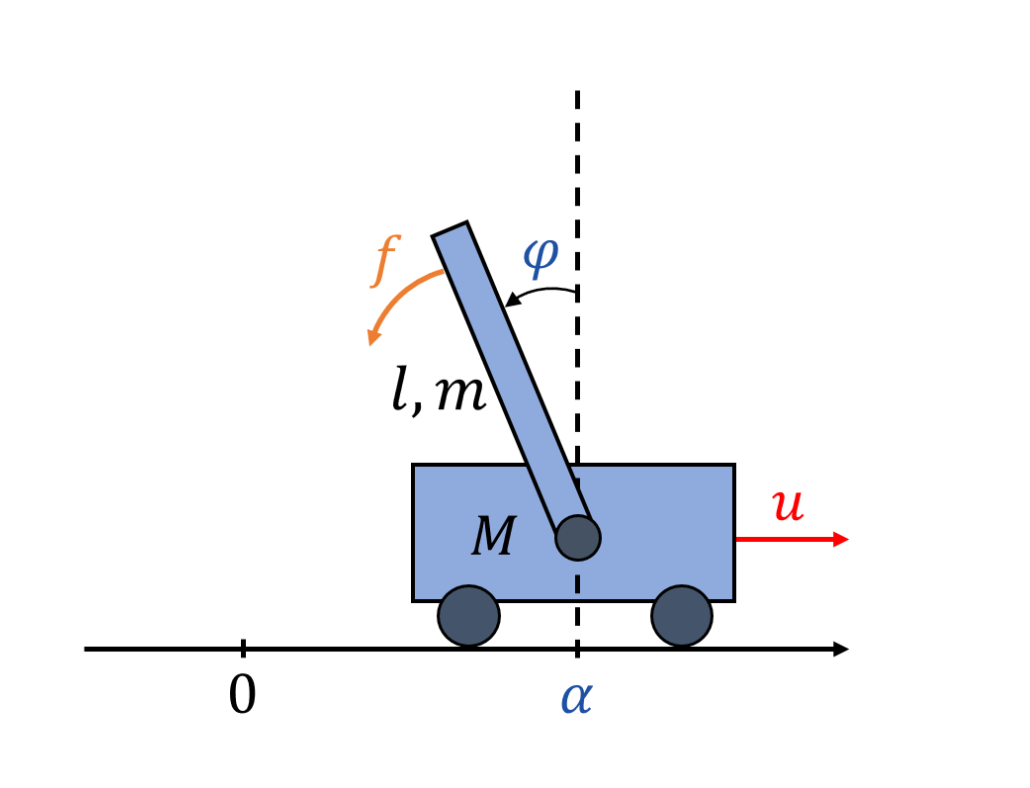
\includegraphics[width=0.5\textwidth]{media/cart.png}
    \caption{Схема маятника на тележке}
    \label{fig:pendulum}
\end{figure}

\subsection{Уравнения движения}
Используем законы Лагранжа для записи уравнений движения системы. 

Так как кинетическая и потенциальная зависят от центра масс тележки и маятника, введем в рассмотрение расстояние $l$ 
от точки подвеса маятника до его центра масс. При этом $l = l_{\text{pend}}/2$ для равномерно распределенной массы маятника.

Напишем уравнения для координат центра масс маятника $x_m$ и $y_m$ и продифференцировав их по времени, получим скорости центра масс маятника:
\begin{equation}
    \begin{cases}
        x_m = x + l\sin\theta, \\
        y_m = l\cos\theta
    \end{cases} \Rightarrow
    \begin{cases}
        v_x = \dot{x} + l\dot{\theta}\cos\theta, \\
        v_y = -l\dot{\theta}\sin\theta
    \end{cases}
\end{equation}
Общая энергия системы складывается из кинетической и потенциальной энергии маятника и кинетической энергии тележки:

Кинетическая энергия системы равна:
\begin{equation}
    T = \frac{1}{2} (M + m)\dot{x}^2 + m\dot{x}l\dot{\theta}\cos\theta + \frac{1}{2}ml^2\dot{\theta}^2
\end{equation}
Потенциальная энергия системы равна:
\begin{equation}
    U = mgl\cos\theta
\end{equation}
Записывая функция Лагранжа $L = T - U$, получаем: 
\begin{equation}
    L = \frac{1}{2} (M + m)\dot{x}^2 + m\dot{x}l\dot{\theta}\cos\theta + \frac{1}{2}ml^2\dot{\theta}^2 - mgl\cos\theta
\end{equation}
Уравнения Лагранжа примут вид:
\begin{equation}
    \begin{array}{cc}
        \frac{d}{dt} \left( \frac{\partial L}{\partial \dot{x}} \right) - \frac{\partial L}{\partial x} = Q_x, \\
        \frac{d}{dt} \left( \frac{\partial L}{\partial \dot{\theta}} \right) - \frac{\partial L}{\partial \theta} = Q_{\theta}
    \end{array}
\end{equation}
где $Q_x$ и $Q_{\theta}$ -- обобщенные силы, действующие на тележку и маятник соответственно. В итоге получаем систему уравнений:
\begin{equation}
    \begin{cases}
        (M + m)\ddot{x} + ml\ddot{\theta}\cos\theta - ml\dot{\theta}^2\sin\theta = Q_x, \\
        ml^2\ddot{\theta} + ml\ddot{x}\cos\theta - mgl\sin\theta = Q_{\theta}.
    \end{cases}
    \label{eq:forces_balance}
\end{equation}
Система уравнений \eqref{eq:forces_balance} представляет собой уравнения баланса сил, 
приложенных к тележке и моментов, действующих на маятник.

Запишем этм уравнения разрешив их относительно высших производных. Заметим, что вторые производные 
входят в эти уравнения линейно. С учетом этого приведем уравнения к матричному виду:  % # TODO: analiz_ustoychivosti_perevernutogo_mayatnika_v_srede_matlab_control
\begin{equation}
    \begin{bmatrix}
        ml^2 & ml\cos\theta \\
        ml\cos\theta & M + m \\
    \end{bmatrix} \times
    \begin{bmatrix}
        \ddot{\theta} \\
        \ddot{x} \\
    \end{bmatrix} =
    \begin{bmatrix}
        mgl\sin\theta + Q_{\theta} \\
        ml\dot{\theta}^2\sin\theta + Q_x
    \end{bmatrix}
\end{equation}
Убедимся в существовании и единственности решения системы:
\begin{equation}
    D = ml^2(M + m) - m^2l^2\cos^2\theta = ml^2(M + m - m\cos^2\theta) > 0
\end{equation}
Решая систему уравнений методом Крамера, получаем:
\begin{multline}
    \Delta_{\ddot{\theta}} = \begin{vmatrix}
        mgl\sin\theta + Q_{\theta} & ml\cos\theta \\
        ml\dot{\theta}^2\sin\theta + Q_x & M + m \\
    \end{vmatrix} = (mgl\sin\theta + Q_{\theta})(M + m) - ml\cos\theta(ml\dot{\theta}^2\sin\theta + Q_x) 
\end{multline}
\begin{multline}
    \Delta_{\ddot{x}} = \begin{vmatrix}
        ml^2 & mgl\sin\theta + Q_{\theta} \\
        ml\cos\theta & ml\dot{\theta}^2\sin\theta + Q_x \\
    \end{vmatrix} = ml^2(ml\dot{\theta}^2\sin\theta + Q_x) - ml\cos\theta(mgl\sin\theta + Q_{\theta})
\end{multline}

\begin{equation}
    \begin{cases}
        \ddot{x} = \frac{ml^2(ml\dot{\theta}^2\sin\theta + Q_x) - ml\cos\theta(mgl\sin\theta + Q_{\theta})}{ml^2(M + m - m\cos^2\theta)} \\ 
        \ddot{\theta} = \frac{(mgl\sin\theta + Q_{\theta})(M + m) - ml\cos\theta(ml\dot{\theta}^2\sin\theta + Q_x)}{ml^2(M + m - m\cos^2\theta)} \\ 
    \end{cases}
    \label{eq:nonlinear_model}
\end{equation}

Можно записать систему в пространстве состояний $X$ в форме Коши: 
\begin{equation}
    \begin{array}{cc}
        X = \begin{bmatrix} 
            x \\
            \dot{x} \\
            \theta \\
            \dot{\theta}
    \end{bmatrix} & 
    \dot{X} = \begin{bmatrix}
        \dot{x} \\
        \frac{ml^2(ml\dot{\theta}^2\sin\theta + Q_x) - ml\cos\theta(mgl\sin\theta + Q_{\theta})}{ml^2(M + m - m\cos^2\theta)}
        \dot{\theta} \\
        \frac{(mgl\sin\theta + Q_{\theta})(M + m) - ml\cos\theta(ml\dot{\theta}^2\sin\theta + Q_x)}{ml^2(M + m - m\cos^2\theta)} \\ 
    \end{bmatrix}
    \end{array}
\end{equation}
Измеряемым выходом системы будет считать вектор $Y$, состоящий из координат тележки и угла отклонения маятника от вертикали:
\begin{equation}
    Y = \begin{bmatrix}
        1 & 0 & 0 & 0 \\
        0 & 0 & 1 & 0 \\ 
    \end{bmatrix} X
\end{equation}

\subsection{Точки равновесия}
Найдем точки равновесия системы в отсутствие внешних сил ($Q_x = Q_{\theta} = 0$). 
Для этого приравняем к нулю правые части уравнений движения, решим систему уравнений:
\begin{equation}
    \dot{X} = 0 \Rightarrow 
    \begin{cases}
        \dot{x} = 0, \\
        \dot{\theta} = 0, \\
        \frac{(mgl\sin\theta + Q_{\theta})(M + m) - ml\cos\theta(ml\dot{\theta}^2\sin\theta + Q_x)}{ml^2(M + m - m\cos^2\theta)} = 0 \\ 
        \frac{ml^2(ml\dot{\theta}^2\sin\theta + Q_x) - ml\cos\theta(mgl\sin\theta + Q_{\theta})}{ml^2(M + m - m\cos^2\theta)} = 0
    \end{cases}
\end{equation}
Упростив, получаем: 
\begin{equation}
    \begin{cases}
        \sin\theta(g(M + m) - \cos\theta(ml)) = 0 \\ 
        \sin\theta(ml - \cos\theta g) = 0
    \end{cases}
\end{equation}
Решая систему уравнений, получаем:
\begin{equation}
    \sin\theta = 0 \Rightarrow \theta = 0, \pi 
\end{equation}
Таким образом, точки равновесия системы определяются углом отклонения маятника от вертикали $\theta = 0$ и $\theta = \pi$, 
что соответствует наивысшему и наинизшему положению маятника соответственно, что сходится с ожидаемым результатом. 

\subsection{Линейная модель}
Для дальнейшего анализа системы ее необходимо линеаризовать. Линеаризацию необходимо проводить в точках равновесия 
системы, которые были найдены в предыдущем пункте, в противном случае отклонения линейной модели от реальной системы будут велики. 
Линеаризуем систему в точке равновесия $\theta = 0$ и $x = 0$, используя то, что $\sin x \approx x$, $\cos x \approx 1$, $x^{n + 1} \approx 0, n \in N$ 
при малых $x$. 
\begin{equation}
    \dot{X} = \begin{bmatrix}
        \dot{x} \\
        \frac{lQ_x - mgl\theta - Q_{\theta}}{lM} \\
        \dot{\theta} \\
        \frac{(g\theta + Q_{\theta})(M + m) -Q_x}{lM} \\ 
    \end{bmatrix}
\end{equation}
Запишем систему в матричном виде, принимая за управление обобщенную силу, приложенную на каретку, а за внешнее 
внешнее возмущение обобщенную силу, приложенную на маятник $u = Q_x, f = Q_{\theta}$:
\begin{equation}
    \begin{cases}
        \dot{x} = Ax + Bu + Df \\ 
        y = Cx
    \end{cases}
    \label{eq:linear_model}
\end{equation}
\begin{equation}
    \begin{array}{cc}
        \begin{bmatrix}
        \dot{x} \\
        \ddot{x} \\
        \dot{\theta} \\
        \ddot{\theta} \\
    \end{bmatrix} = \begin{bmatrix}
        0 & 1 & 0 & 0 \\
        0 & 0 & \frac{-mg}{M} & 0 \\
        0 & 0 & 0 & 1 \\
        0 & 0 & \frac{g(M + m)}{lM} & 0 \\
    \end{bmatrix} \times \begin{bmatrix}
        x \\
        \dot{x} \\
        \theta \\
        \dot{\theta} \\
    \end{bmatrix} + \begin{bmatrix}
        0 \\
        \frac{1}{M} \\
        0 \\
        \frac{-1}{lM} \\
    \end{bmatrix} \times Q_x + \begin{bmatrix}
        0 \\
        \frac{-1}{lM} \\
        0 \\
        \frac{M + m}{lM} \\ 
    \end{bmatrix} \times Q_{\theta}  \\[4em]
    y = \begin{bmatrix}
        1 & 0 & 0 & 0 \\
        0 & 0 & 1 & 0 \\ 
    \end{bmatrix} \times \begin{bmatrix}
        x \\
        \dot{x} \\
        \theta \\
        \dot{\theta} \\
    \end{bmatrix}
    \end{array}
\end{equation}
Таким образом, матрицы системы примут вид: 
\begin{equation}
    A = \begin{bmatrix}
        0 & 1 & 0 & 0 \\
        0 & 0 & \frac{-mg}{M} & 0 \\
        0 & 0 & 0 & 1 \\
        0 & 0 & \frac{g(M + m)}{lM} & 0 \\
    \end{bmatrix}, B = \begin{bmatrix}
        0 \\
        \frac{1}{M} \\
        0 \\
        \frac{-1}{lM} \\
    \end{bmatrix}, D = \begin{bmatrix}
        0 \\
        \frac{-1}{lM} \\
        0 \\
        \frac{M + m}{lM} \\ 
    \end{bmatrix}, C = \begin{bmatrix}
        1 & 0 & 0 & 0 \\
        0 & 0 & 1 & 0 \\ 
    \end{bmatrix}
\end{equation}

\FloatBarrier
\section{Анализ математический модели}
\subsection{Устойчивость системы} 
Для дальнейшего анализа системы выберем случайным образом параметры системы:
\begin{equation}
    M = 255.169,\quad m = 8.328,\quad l = 0.769
\end{equation}
Подставив эти значения в матрицы системы (\ref{eq:linear_model}), получаем: 
\begin{equation}
    A = \begin{bmatrix}
    0.00  & 1.00  & 0.00  & 0.00 \\ 
    0.00  & 0.00  & 0.32  & 0.00 \\ 
    0.00  & 0.00  & 0.00  & 1.00 \\ 
    0.00  & 0.00  & 26.34  & 0.00 \\ 
    \end{bmatrix},
    B = \begin{bmatrix}
    0.0000 \\ 
    0.0039 \\ 
    0.0000 \\ 
    0.0102 \\ 
    \end{bmatrix},
    C = \begin{bmatrix}
    1  & 0  & 0  & 0 \\ 
    0  & 0  & 1  & 0 \\ 
    \end{bmatrix},
    D = \begin{bmatrix}
    0.000 \\ 
    0.010 \\ 
    0.000 \\ 
    0.838 \\ 
    \end{bmatrix}
\end{equation}

Проведем анализ полученный системы. Для этого, в первую очередь, найдем собственные числа матрицы $A$. 
\begin{equation}
    \sigma(A) \begin{bmatrix}
    0.00 \\ 
    0.00 \\ 
    5.13 \\ 
    -5.13 \\ 
    \end{bmatrix}
\end{equation}
В матрице системы есть два нулевых собственных числа, один отрицательный (устойчивый) и один положительный (неустойчивый). 
Наличие хотя бы одного положительного собственного числа говорит о том, что система неустойчива. При этом 
наличие двух нулевых собственных чисел свидетельствует о колебательной природе системы. 

Найдем собственные векторы матрицы $A$:
\begin{equation}
    V_1 = \begin{bmatrix}
    1.00  \\ 0.00  \\ 0.00 \\ 0.00 \\
    \end{bmatrix}^T,\quad
    V_2 = \begin{bmatrix}
    -1.00 \\ 0.00 \\ 0.00 \\ 0.00 \\
    \end{bmatrix}^T,\quad
    V_3 = \begin{bmatrix}
    0.00 \\ 0.01 \\ 0.19 \\ 0.98 \\
    \end{bmatrix}^T,\quad
    V_4 = \begin{bmatrix}
    0.00  \\ 0.01  \\ -0.19 \\ 0.98 \\
    \end{bmatrix}^T
    \label{eq:eigenvectors}
\end{equation}
Собственные векторы линейной системы показывают, в каких \textit{направлениях} двигаются отдельные моды системы. 
Так, первый два вектора, соответствующие нулевым собственным числам, показывают, что система может иметь различные
линейные координаты вдоль оси $x$, при этом не изменяя угол отклонения маятника, его скорость. В то время как третий и четвертый
векторы показывают, что изменение скорости тележки, угла отклонения маятника и его угловой скорости будут действовать 
друг на друга. 

\subsubsection{Управляемость системы}
Найдем матрицу управляемости системы $U$ и определим ее ранг. 
\begin{equation}
    U = [B, AB, A^2B, A^3B]
\end{equation}
\begin{equation}
    U = \begin{bmatrix}
    0.0000  & 0.0039  & 0.0000  & 0.0033 \\ 
    0.0039  & 0.0000  & 0.0033  & 0.0000 \\ 
    0.0000  & 0.0102  & 0.0000  & 0.2684 \\ 
    0.0102  & 0.0000  & 0.2684  & 0.0000 \\ 
    \end{bmatrix}, \quad \text{Rank}(U) = 4
    \label{eq:controlability_matrix}
\end{equation}
Поскольку ранг матрицы управляемости равен количеству переменных системы, то система является полностью управляемой. 
Поскольку система является полностью управляемой, то нет необходимости проверять управляемость каждого собственного 
числа по отдельности. 

\subsubsection{Наблюдаемость системы}
Найдем матрицу наблюдаемости системы $W$ и определим ее ранг.
\begin{equation}
    W = \begin{bmatrix}
    C \\ 
    CA \\ 
    CA^2 \\ 
    CA^3 \\ 
    \end{bmatrix}
\end{equation}
\begin{equation}
   W = \begin{bmatrix}
    1.0000  & 0.0000  & 0.0000  & 0.0000 \\ 
    0.0000  & 0.0000  & 1.0000  & 0.0000 \\ 
    0.0000  & 1.0000  & 0.0000  & 0.0000 \\ 
    0.0000  & 0.0000  & 0.0000  & 1.0000 \\ 
    0.0000  & 0.0000  & 0.3202  & 0.0000 \\ 
    0.0000  & 0.0000  & 26.3392  & 0.0000 \\ 
    0.0000  & 0.0000  & 0.0000  & 0.3202 \\ 
    0.0000  & 0.0000  & 0.0000  & 26.3392 \\ 
    \end{bmatrix}, \quad \text{Rank}(W) = 4
    \label{eq:observability_matrix}
\end{equation}
Поскольку ранг матрицы наблюдаемости равен количеству переменных системы, то система является полностью наблюдаемой, так же 
пропустим этап проверки наблюдаемости каждого собственного числа по отдельности. 

\subsubsection{Итоги анализа}
В ходе анализа линеаризованной около верхней точки равновесия системы было установлено, что система является
неустойчивой из-за наличия одного положительного собственного числа и двух нулевых собственных чисел, при этом 
система является полностью управляемой и наблюдаемой, что дает возможность синтезировать регуляторы для 
данной системы. 

\subsection{Передаточные функции}
Так как выход системы являются вектором размерности 2, то передаточная функция (матрица) $W_{u\rightarrow y}(s)$ по 
управлению $u(t)$ и выходу $y(t)$ и передаточная функция (матрица) $W_{f\rightarrow y}(s)$ по 
возмущению $f(t)$ и выходу $y(t)$ системы будут иметь размерность $2 \times 1$ и могут быть получены из матричного уравнения состояния
(\ref{eq:linear_model}) системы следующим образом:

Полагая нулевые начальные условия, применим преобразование Лапласа к обеим частям уравнения (\ref{eq:linear_model}): 
\begin{equation}
    \begin{cases}
        sX(s) = AX(s) + BU(s) + DF(s) \\ 
        Y(s) = CX(s)
    \end{cases}
\end{equation}
где $X(s)$, $Y(s)$ и $U(s)$, $F(s)$ - образы Лапласа, соответствующие вектору состояния $x(t)$, выходу $y(t)$ и входу $u(t)$, $f(t)$ системы соответственно.

Разрешим систему относительно $X(s)$:
\begin{equation}
    X(s) = (sI - A)^{-1}BU(s) + (sI - A)^{-1}DF(s)
\end{equation}
Подставим полученное выражение в уравнение для выхода $Y(s)$:
\begin{equation}
    Y(s) = C(sI - A)^{-1}BU(s) + C(sI - A)^{-1}DF(s)
\end{equation}

Теперь, полагая $U(s) = 0$ и $F(s) = 0$ получим передаточные матрицы системы по входу и внешнему возмущению соответственно:
\begin{equation}
    W_{u\rightarrow y}(s) = C(sI - A)^{-1}B
\end{equation}
\begin{equation}
    W_{f\rightarrow y}(s) = C(sI - A)^{-1}D
\end{equation}

Подставив в уравнения полученные ранее матрицы $A$, $B$, $C$ и $D$ получим: 
\begin{equation}
    W_{u \rightarrow y}(s) = \begin{bmatrix}
    \frac{0.0039s^2 - 0.1}{s^4 - 26.3392s^2} \\ 
    \frac{0.0102}{s^2 - 26.3392}
    \end{bmatrix}
\end{equation}
\begin{equation}
    W_{f \rightarrow y}(s) = \begin{bmatrix}
    \frac{0.0102s^2}{s^4 -26.3392s^2} \\ 
    \frac{0.8383}{s^2 - 26.3392}
    \end{bmatrix}
\end{equation}
Определим динамические порядки полученных передаточных функций. 
Принимая то, что динамический порядок системы с несколькими выходами определяется как 
наибольший из динамических порядков передаточных функций звеньев, получаем, 
для первой передаточной функции $W_{u \rightarrow y}(s)$ динамический порядок равен 4, 
для второй передаточной функции $W_{f \rightarrow y}(s)$ динамический порядок равен 4. 
Относительный динамический порядок для всех выходов обоих передаточных функций равен 2. 
Динамический порядок равный 4 указывает на то, что для описание системы требуется 

4 уравнения первого порядка. 

Определим нули и полюса полученных передаточных функций. Для этого найдем корни полиномов числителя и знаменателя 
полученных передаточных функций. 
Полюса обоих передаточных функций соответствуют собственным числам матрицы $A$ и равны:
\begin{equation}
    \begin{array}{cccc}
        \sigma(W_{u \rightarrow y_1}(s)) = \begin{bmatrix}
        0.00 \\ 
        0.00 \\ 
        5.13 \\ 
        -5.13 \\ 
        \end{bmatrix}  & 
        \sigma(W_{u \rightarrow y_2}(s)) = \begin{bmatrix}
        5.13 \\ 
        -5.13 \\ 
        \end{bmatrix} \\[4em]
        \sigma(W_{f \rightarrow y_1}(s)) = \begin{bmatrix}
        0.00 \\ 
        0.00 \\ 
        5.13 \\ 
        -5.13 \\ 
        \end{bmatrix}  & 
        \sigma(W_{f \rightarrow y_2}(s)) = \begin{bmatrix}
        5.13 \\ 
        -5.13 \\ 
        \end{bmatrix} \\ 
    \end{array}
\end{equation}
Нули первой передаточной функции $W_{u \rightarrow y_1}(s)$ равны $\pm 5.06$, 
для второй передаточной функции $W_{u \rightarrow y_2}(s)$ один ноль, равный $0$. Наличие 
нуля в правой полуплоскости указывает на то, что система не является минимальной фазовой. 


\subsection{Моделирование систем}
Создадим блоки, имитирующие поведение начальной системы (\ref{eq:nonlinear_model}) и ее линеаризованной модели (\ref{eq:linear_model})
в среде MATLAB Simulink. На вход блоков будут подаваться управляющее воздействие $u(t)$ и внешнее возмущение $f(t)$, 
а на выходе будет получаться вектор измеряемых величин $y(t)$ и вектора состояния системы, который может быть 
использован в процессе синтеза и проверки регуляторов. В реальной системе он недоступен для непосредственного измерения.
Схемы блоков представлены на рисунке \ref{fig:scheme_unlinear} и \ref{fig:scheme_linear}. 

\begin{figure}[ht!]
    \centering
    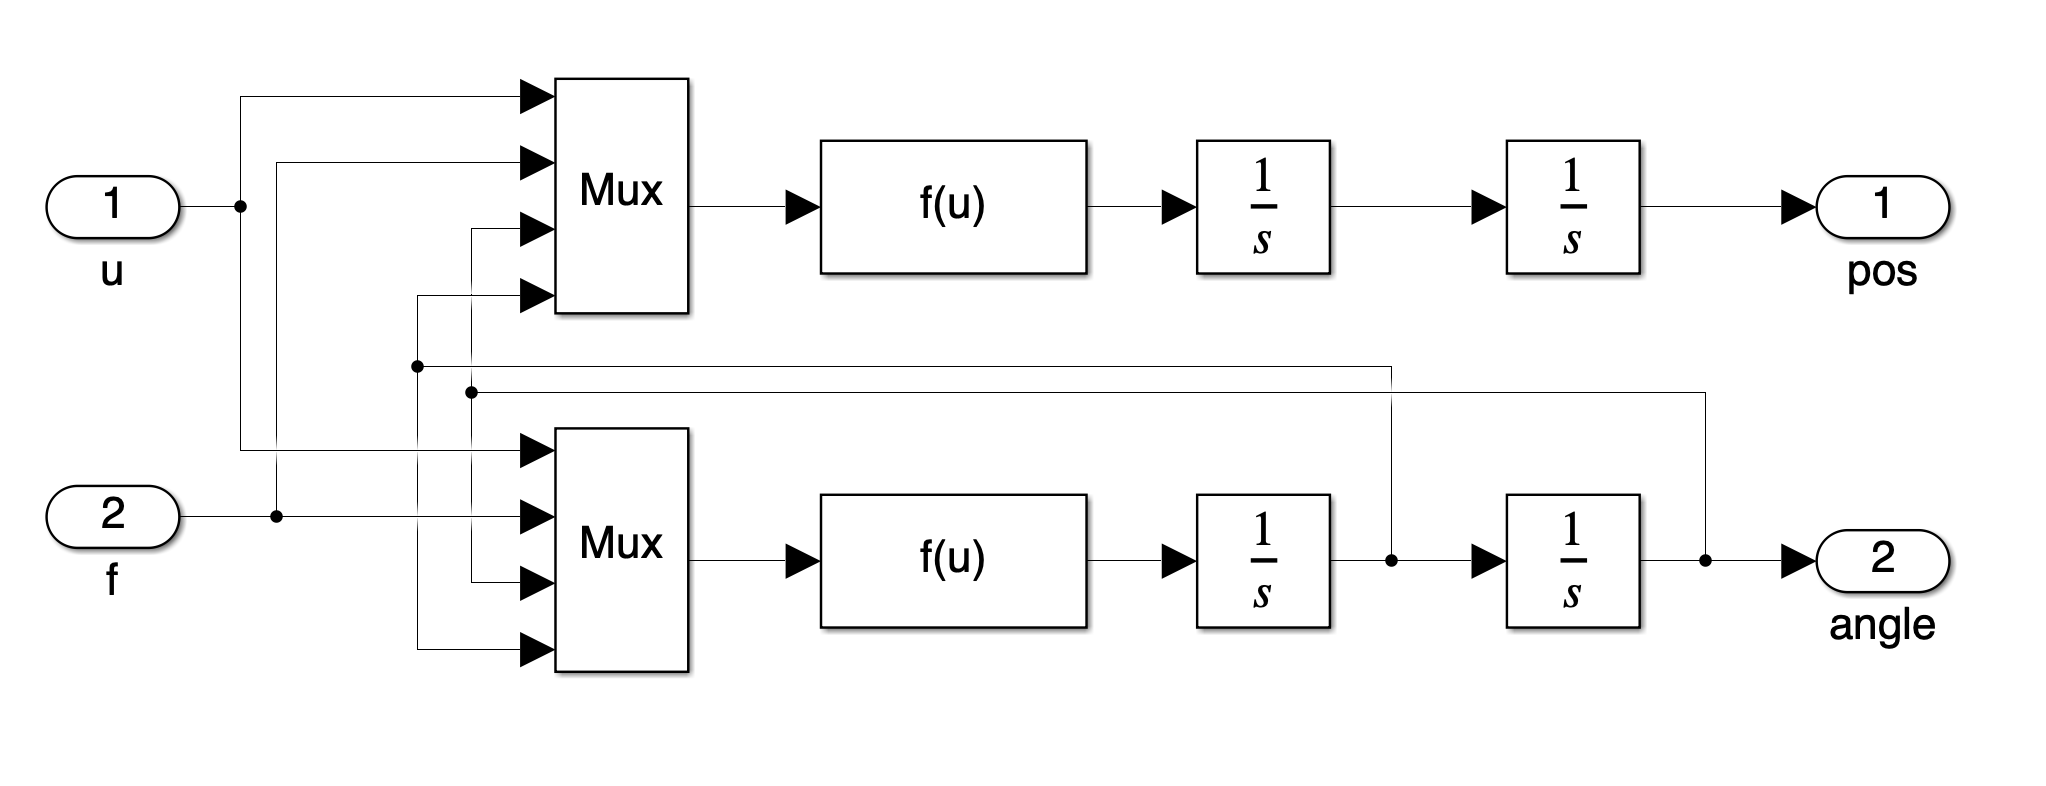
\includegraphics[width=0.8\textwidth]{media/scheme_unlinear.png}
    \caption{Схема блока нелинейной модели системы}
    \label{fig:scheme_unlinear}
\end{figure}
Уравнения в блоках \texttt{fcn} представляют собой уравнения (\ref{eq:nonlinear_model}) системы. 

\begin{figure}[ht!]
    \centering
    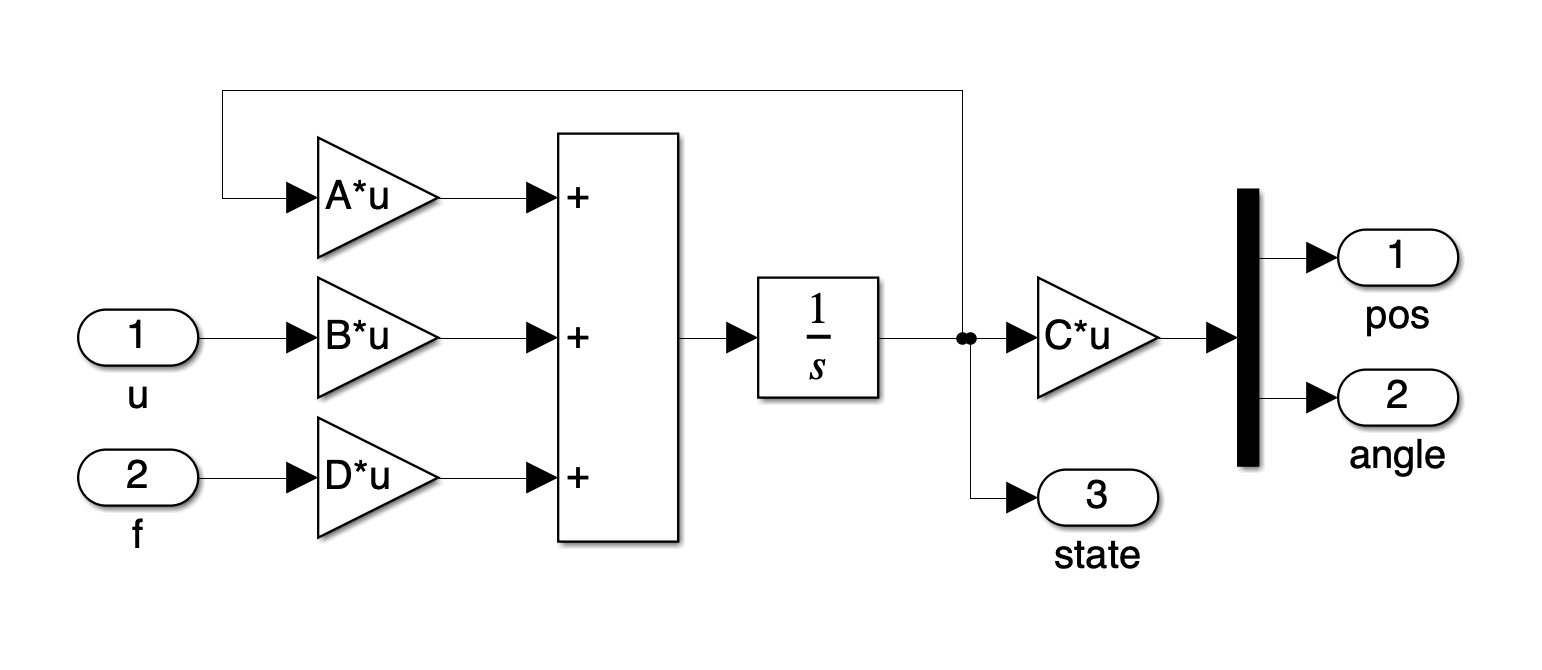
\includegraphics[width=0.8\textwidth]{media/scheme_linear.png}
    \caption{Схема блока линейной модели системы}
    \label{fig:scheme_linear}
\end{figure}

Проведем моделирование свободного движения системы в отсутствии внешнего 
возмущения с различными начальными условиями: будем изменять 
начальное положение маятника (его отклонение от верхнего положения равновесия), все остальные параметры 
системы оставим равными нулю. В качестве начального условия выберем угол отклонения маятника из множества 
$[0, 0.1, -0.1, 0.3, \nicefrac{\pi}{2}, \pi]$. Результаты моделирования представлены на
рисунке \ref{fig:free_motion_nonlinear} и \ref{fig:free_motion_linear}.
\begin{figure}[ht!]
    \centering
    \begin{subfigure}[b]{0.45\textwidth}
        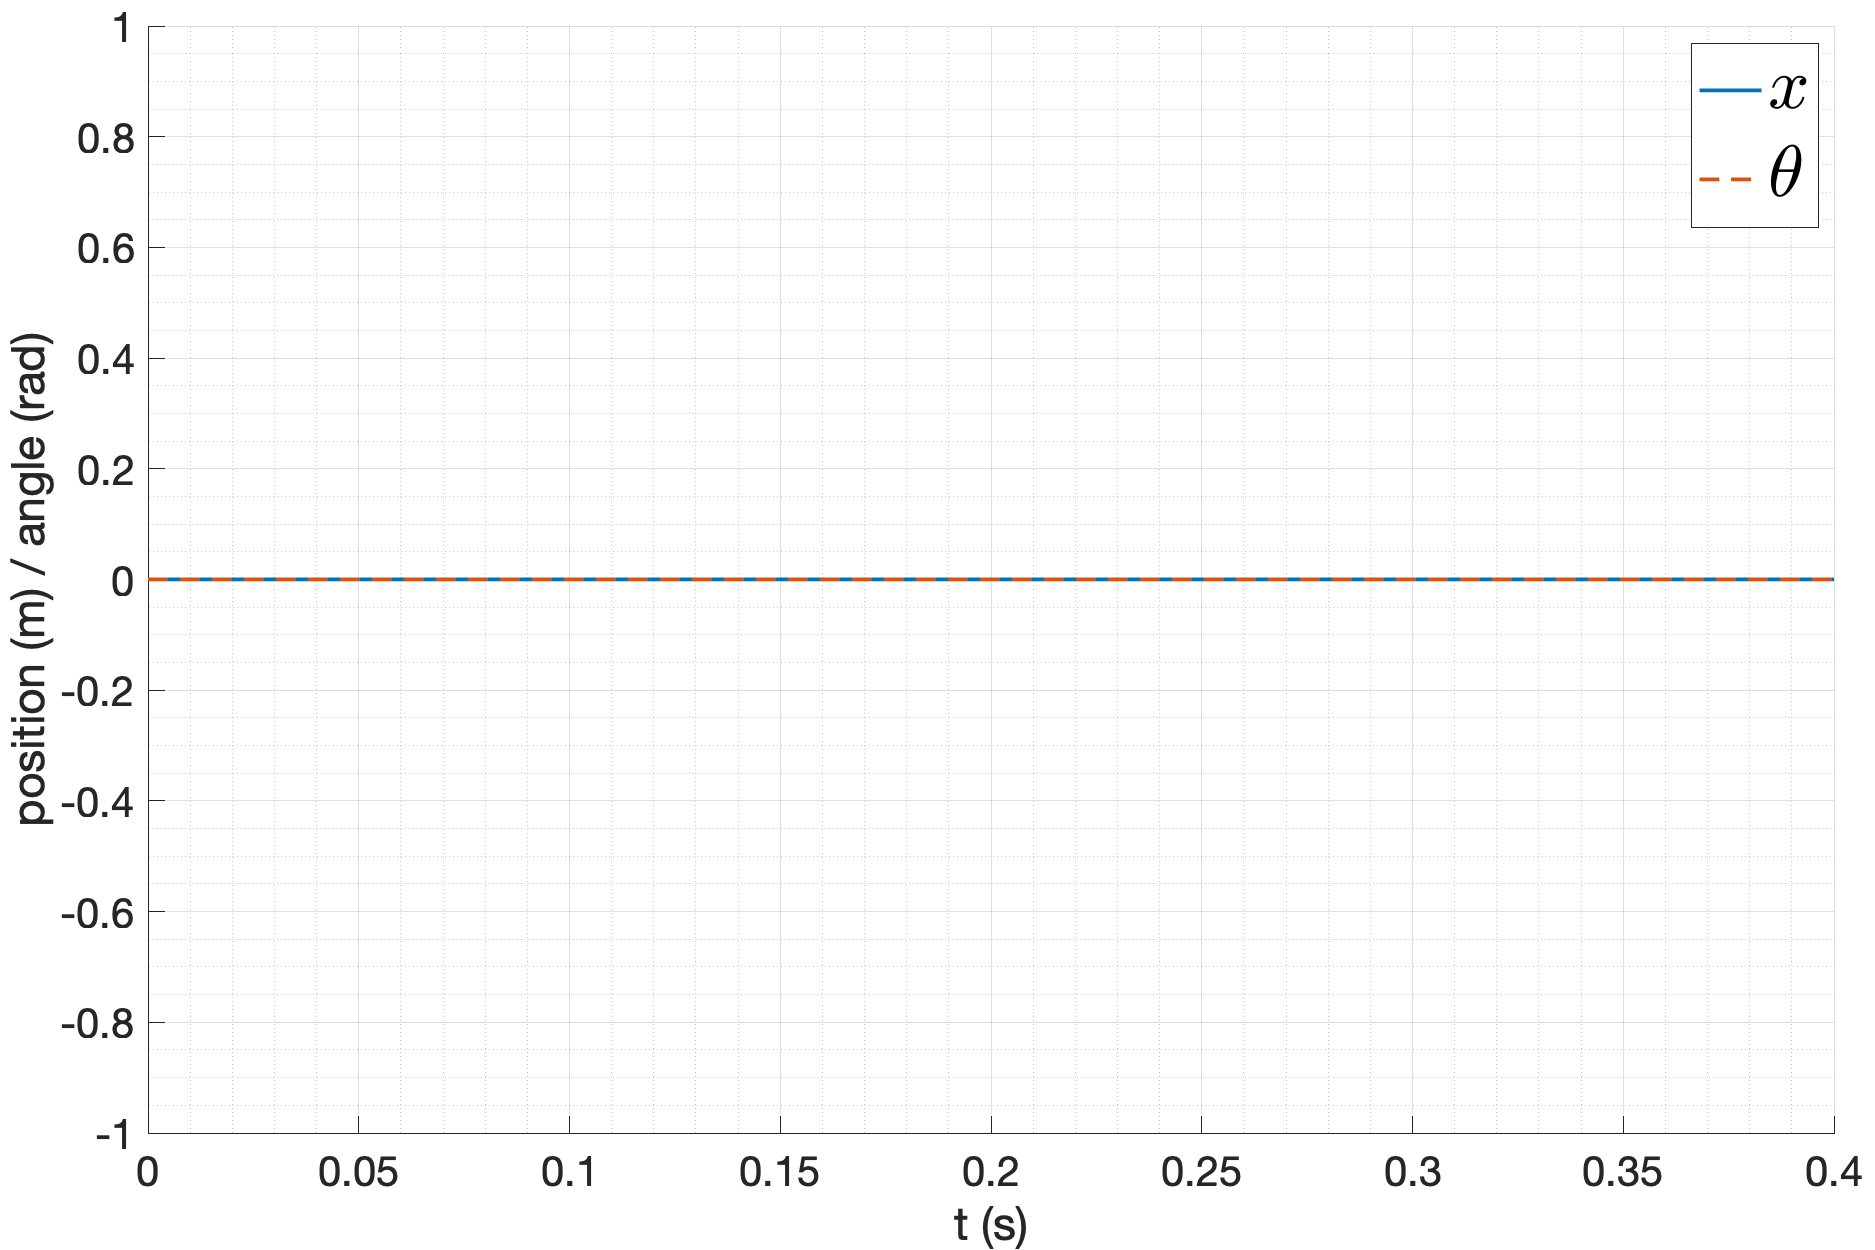
\includegraphics[width=\textwidth]{media/plots/free_motion/nonlin_1.png}
        \caption{$\theta_0 = 0$}
  \end{subfigure}
    \begin{subfigure}[b]{0.45\textwidth}
        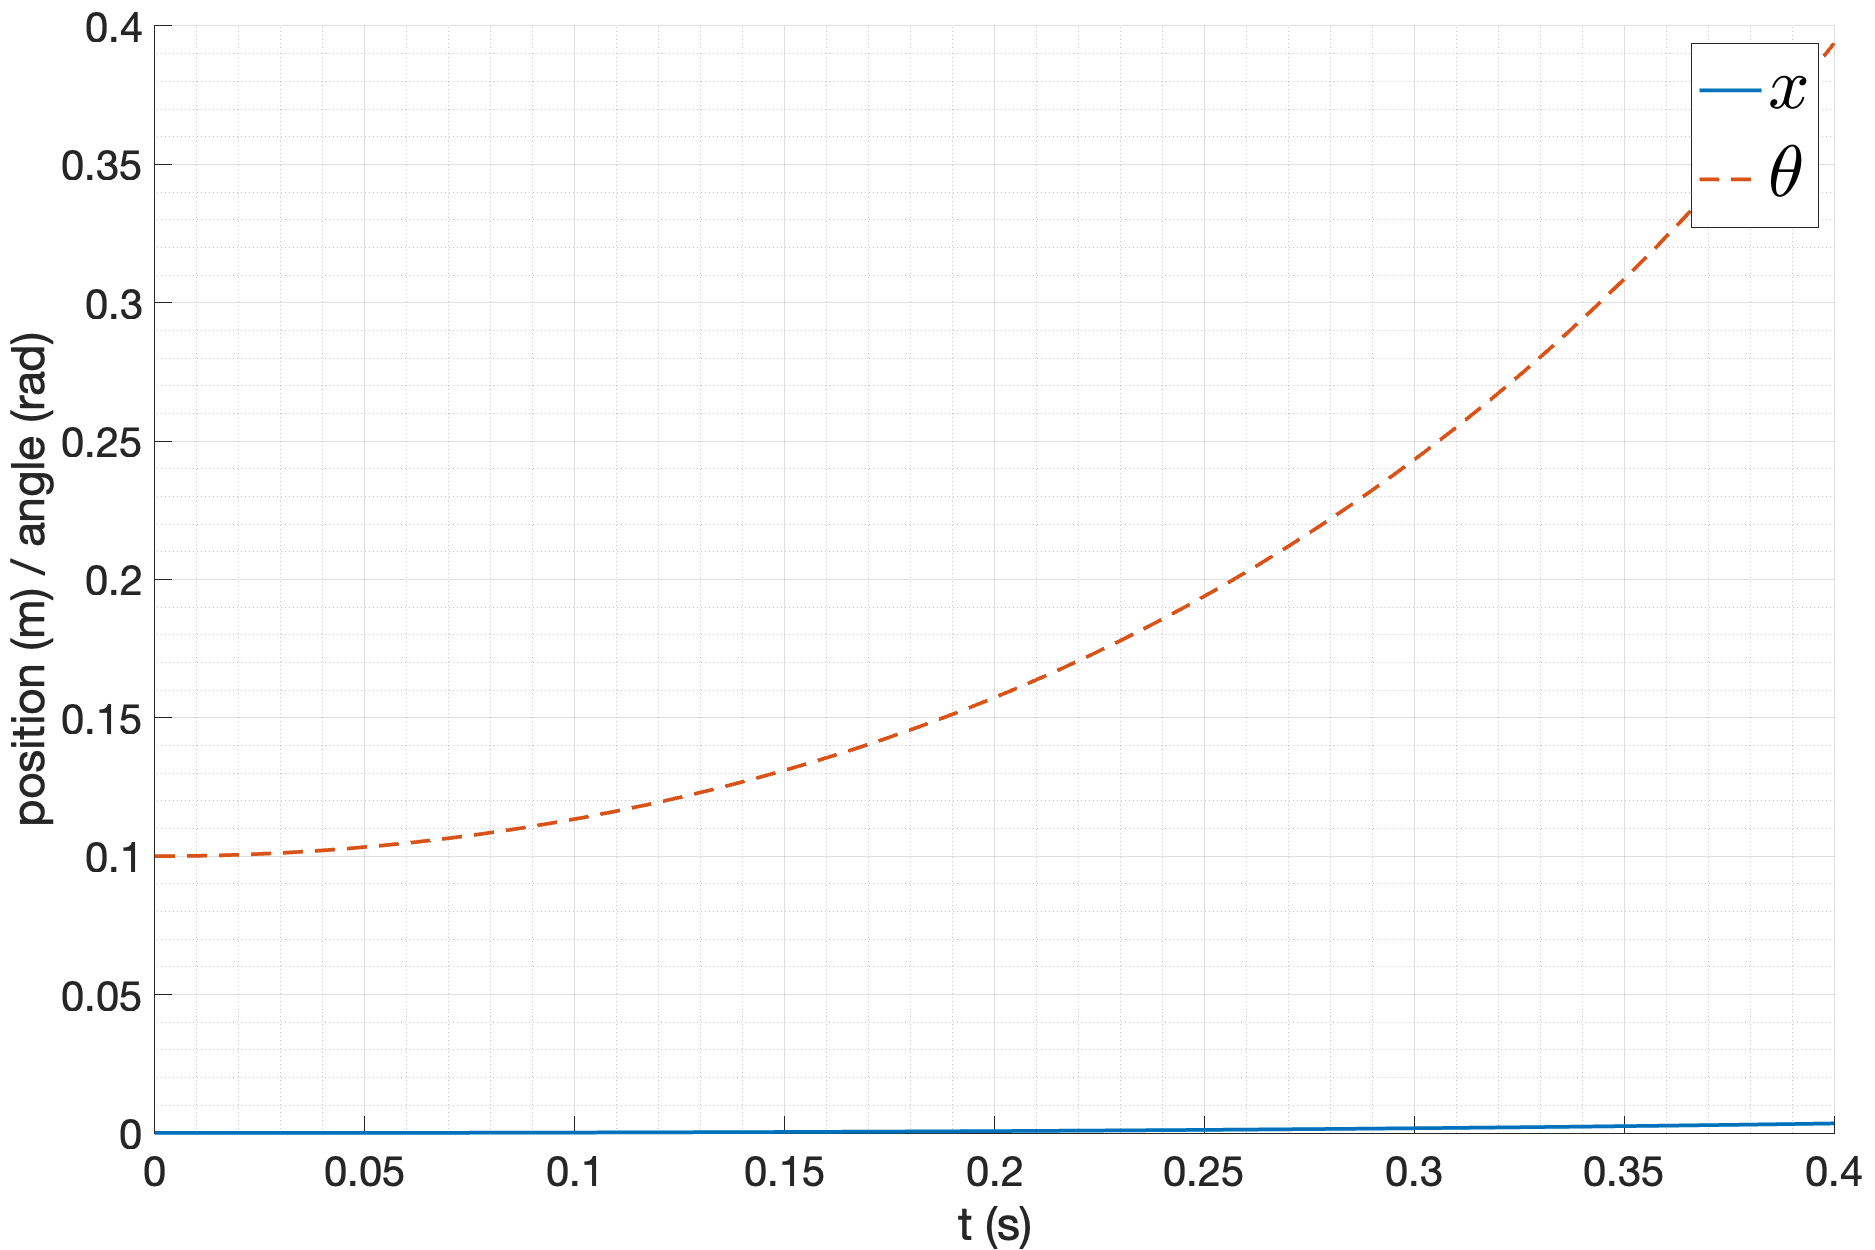
\includegraphics[width=\textwidth]{media/plots/free_motion/nonlin_2.png}
        \caption{$\theta_0 = 0.1$}
    \end{subfigure}
    \begin{subfigure}[b]{0.45\textwidth}
        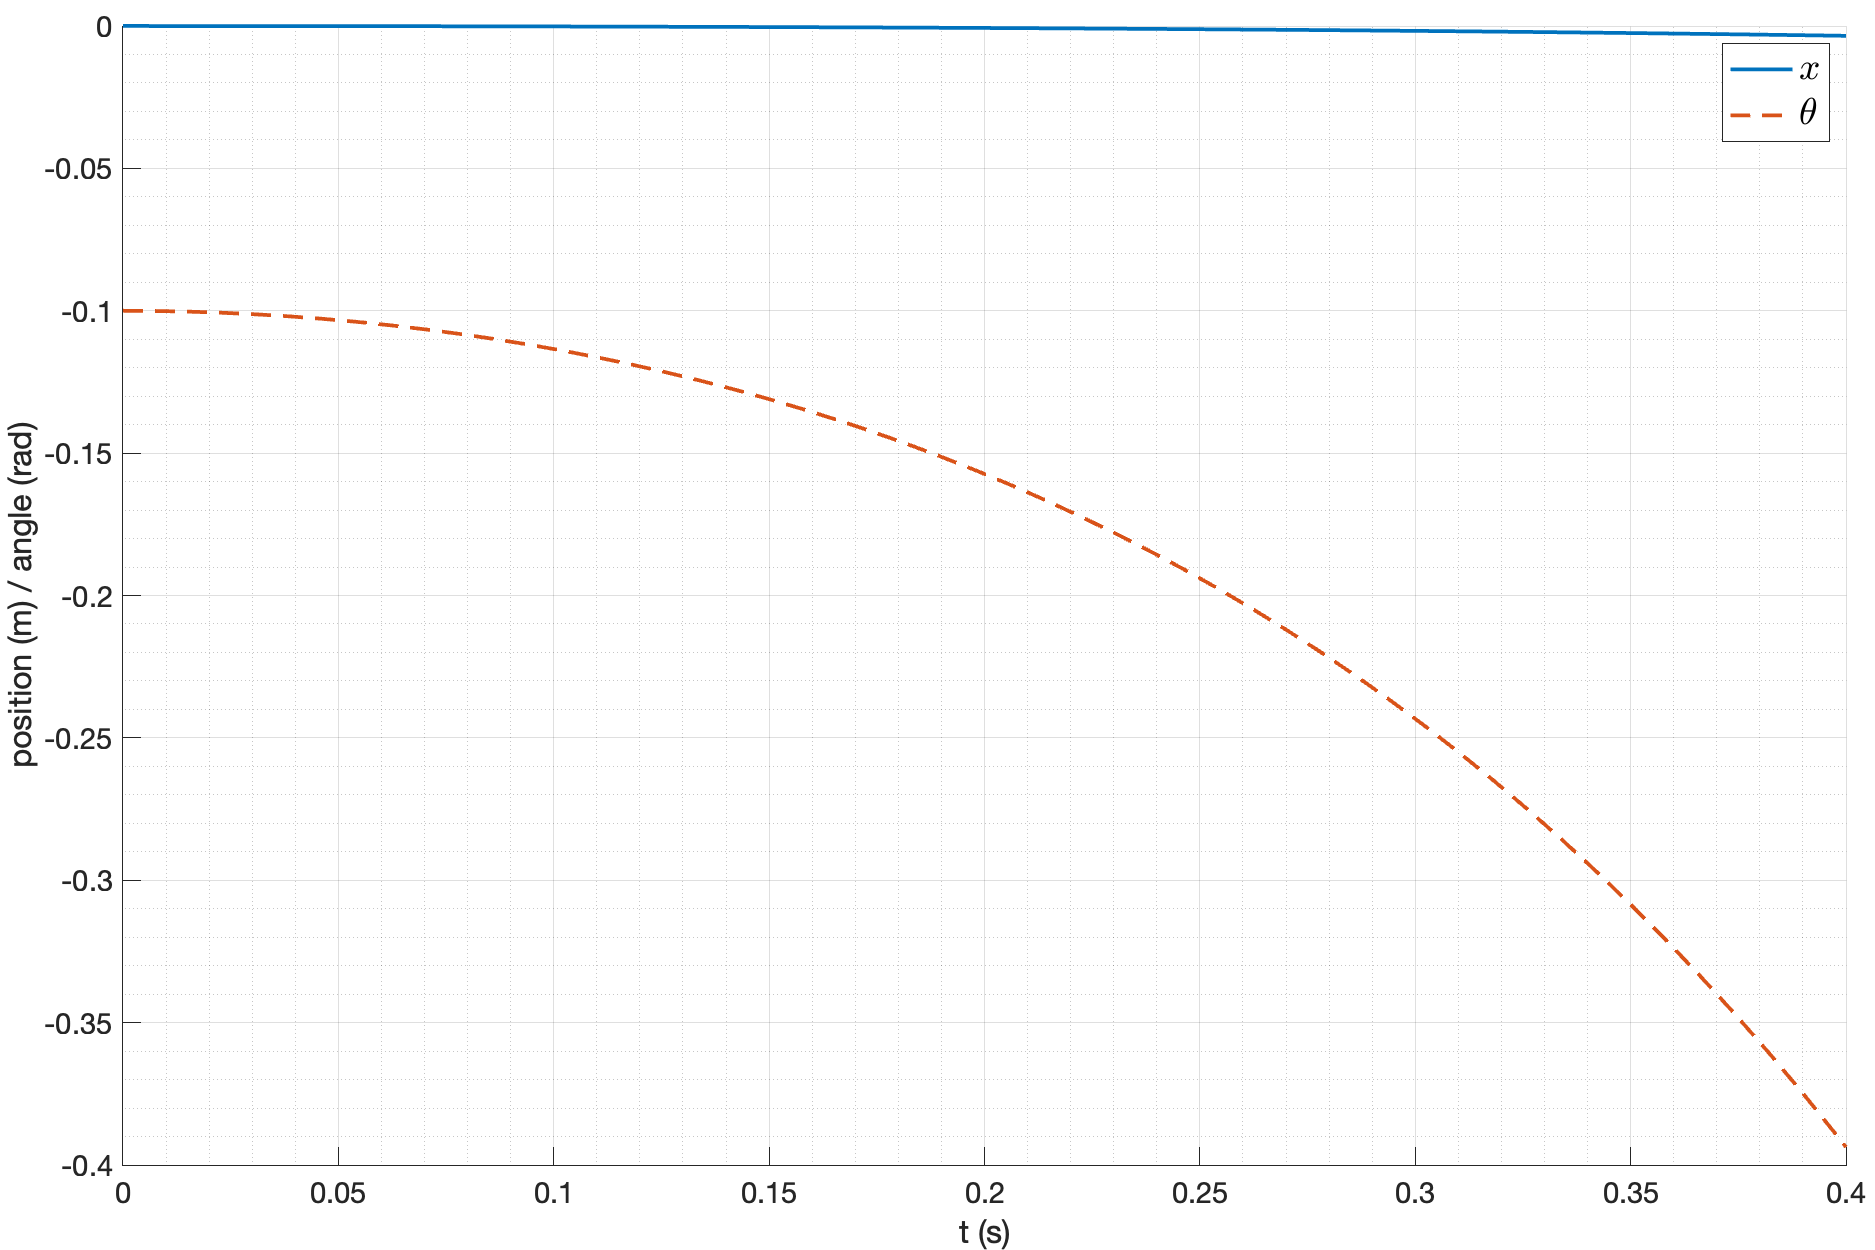
\includegraphics[width=\textwidth]{media/plots/free_motion/nonlin_3.png}
        \caption{$\theta_0 = -0.1$}
    \end{subfigure}
    \begin{subfigure}[b]{0.45\textwidth}
        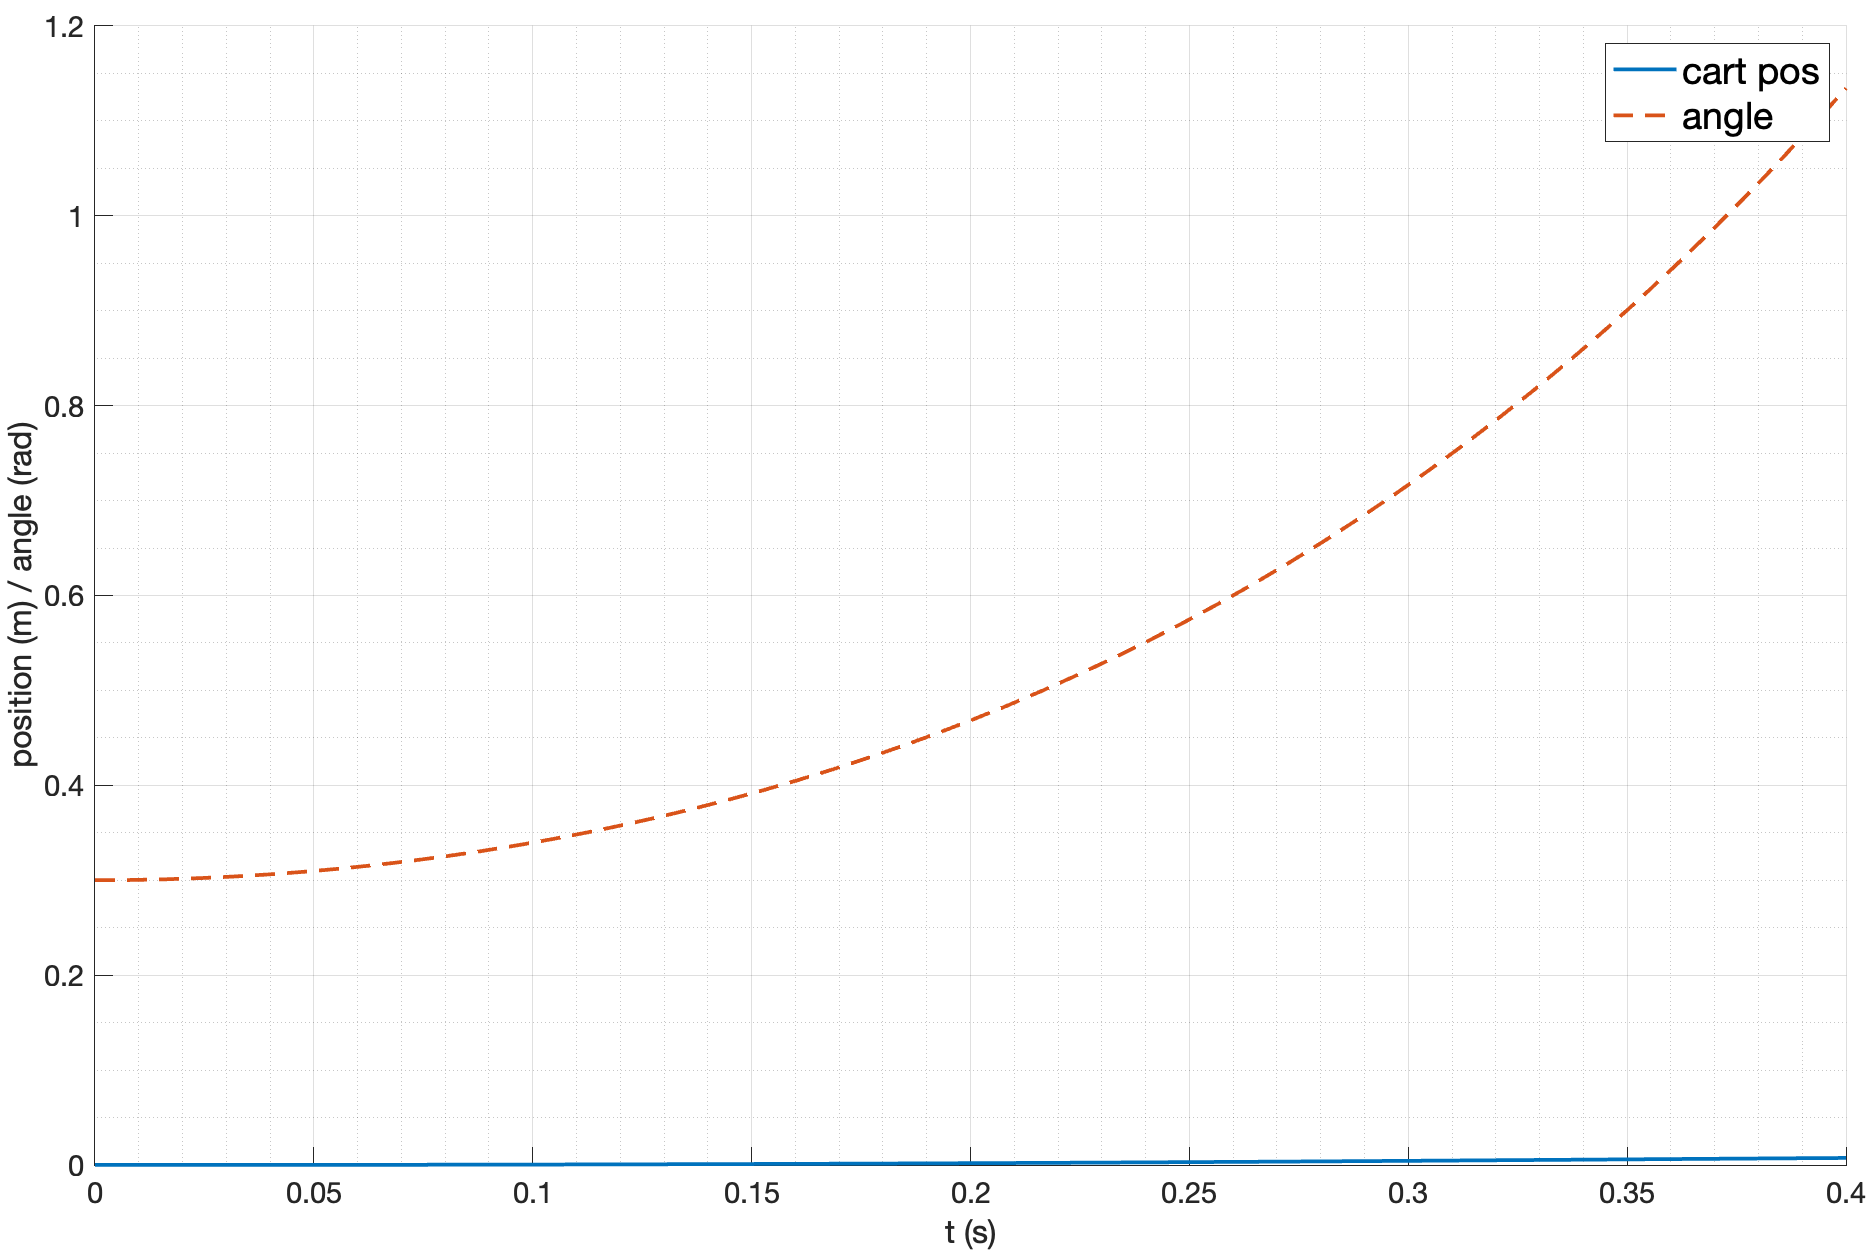
\includegraphics[width=\textwidth]{media/plots/free_motion/nonlin_4.png}
        \caption{$\theta_0 = 0.3$}
    \end{subfigure}
    \begin{subfigure}[b]{0.45\textwidth}
        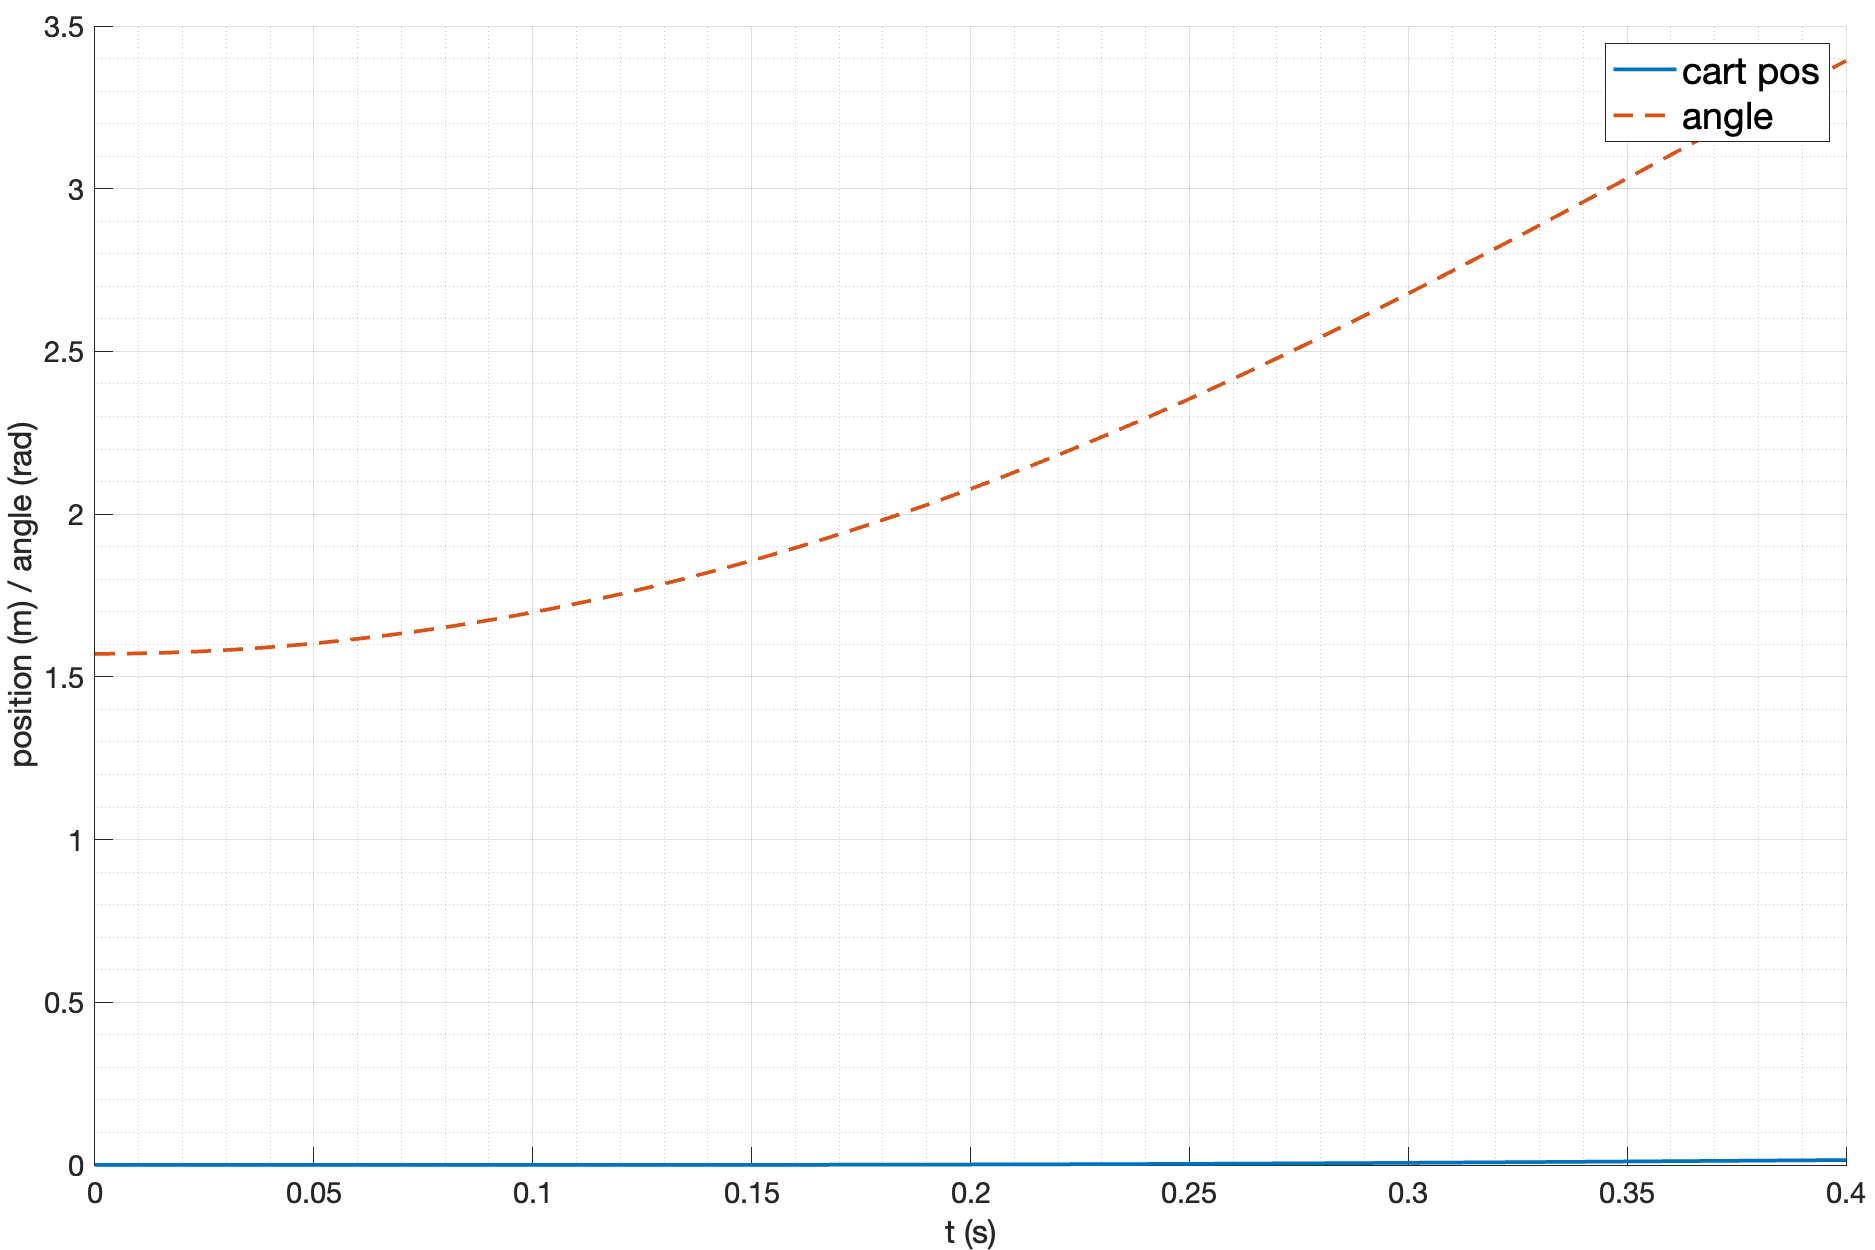
\includegraphics[width=\textwidth]{media/plots/free_motion/nonlin_5.png}
        \caption{$\theta_0 = \frac{\pi}{2}$}
    \end{subfigure}
    \begin{subfigure}[b]{0.45\textwidth}
        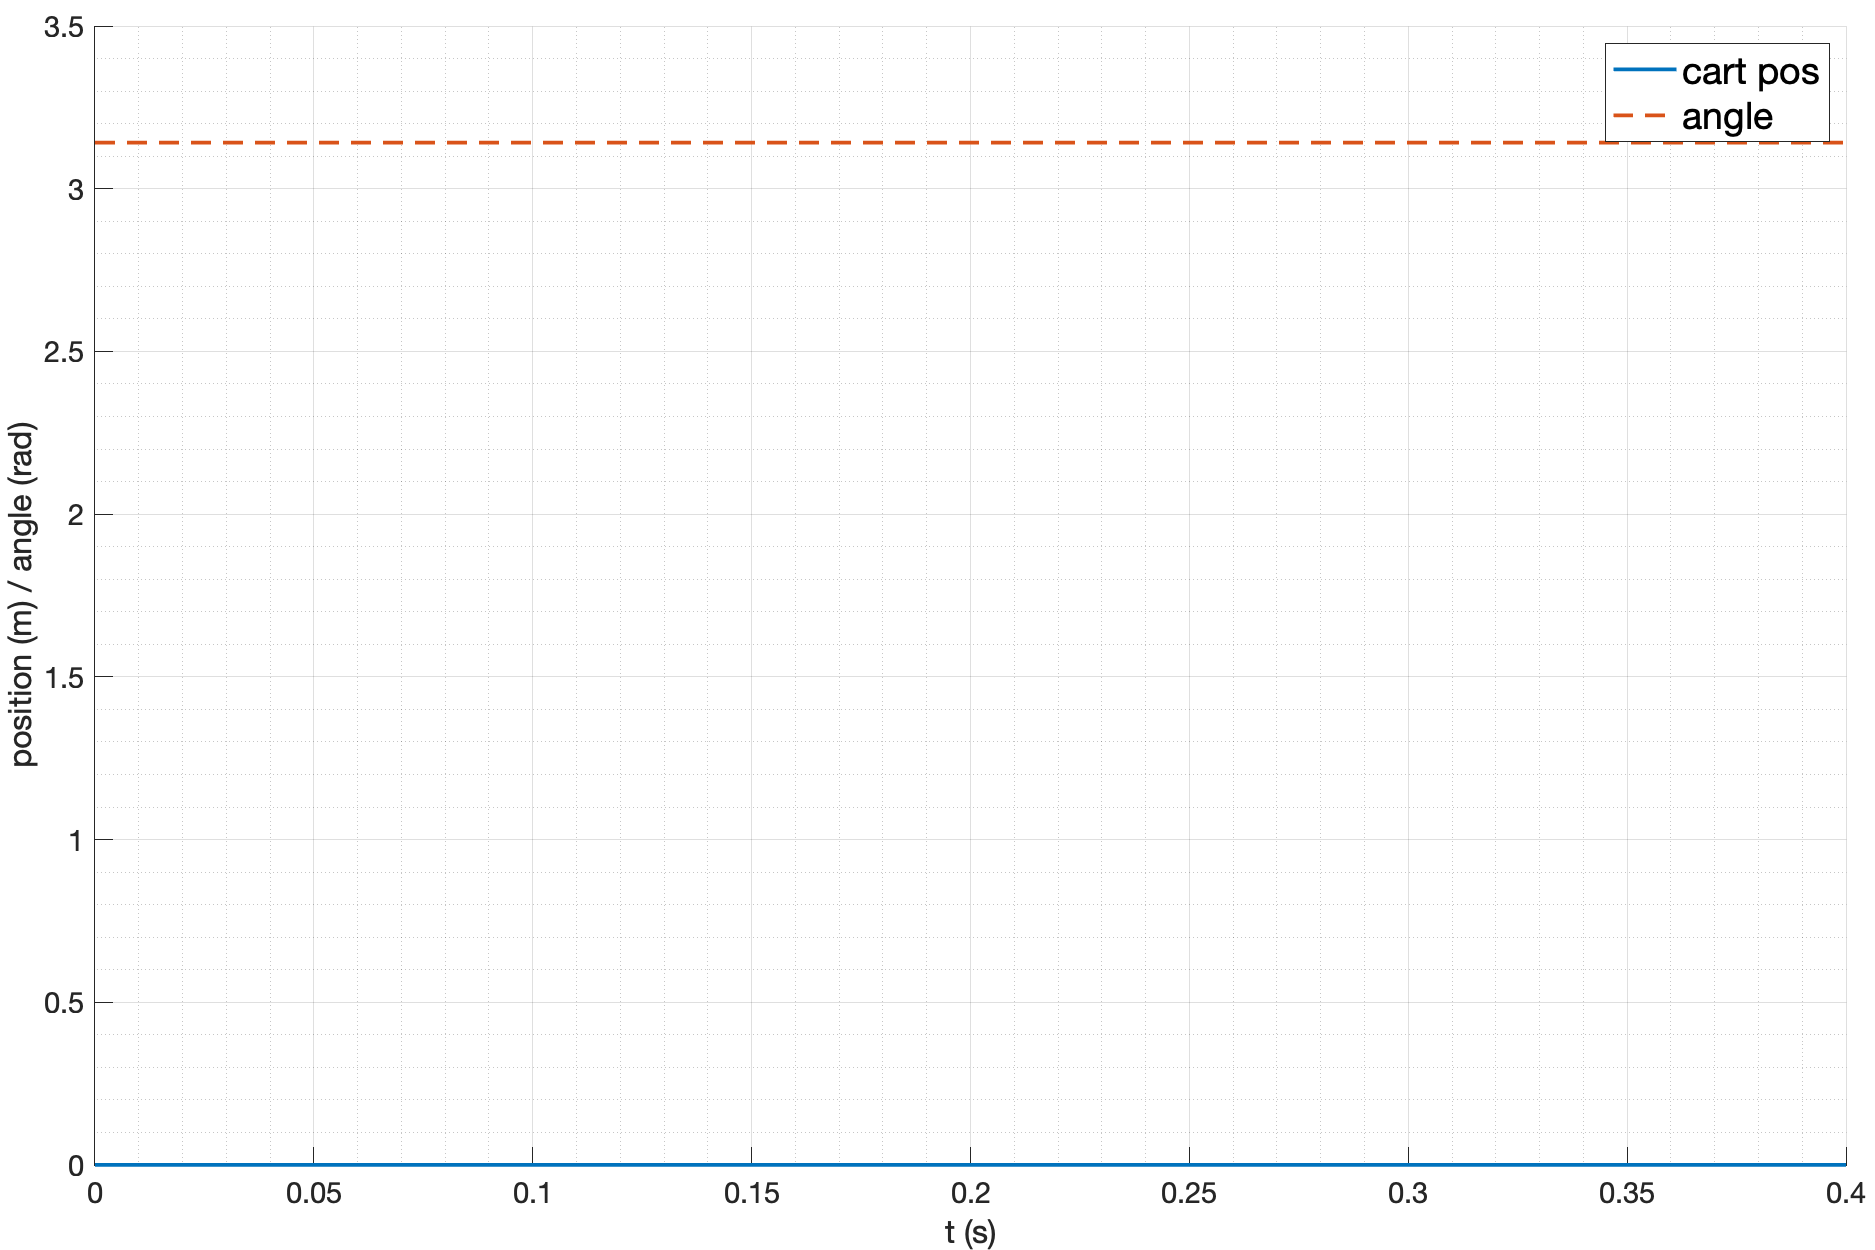
\includegraphics[width=\textwidth]{media/plots/free_motion/nonlin_6.png}
        \caption{$\theta_0 = \pi$}
    \end{subfigure}
    \caption{Свободное движение маятника (нелинейная модель)}
    \label{fig:free_motion_nonlinear}
\end{figure}

\begin{figure}[ht!]
    \centering
    \begin{subfigure}[b]{0.45\textwidth}
        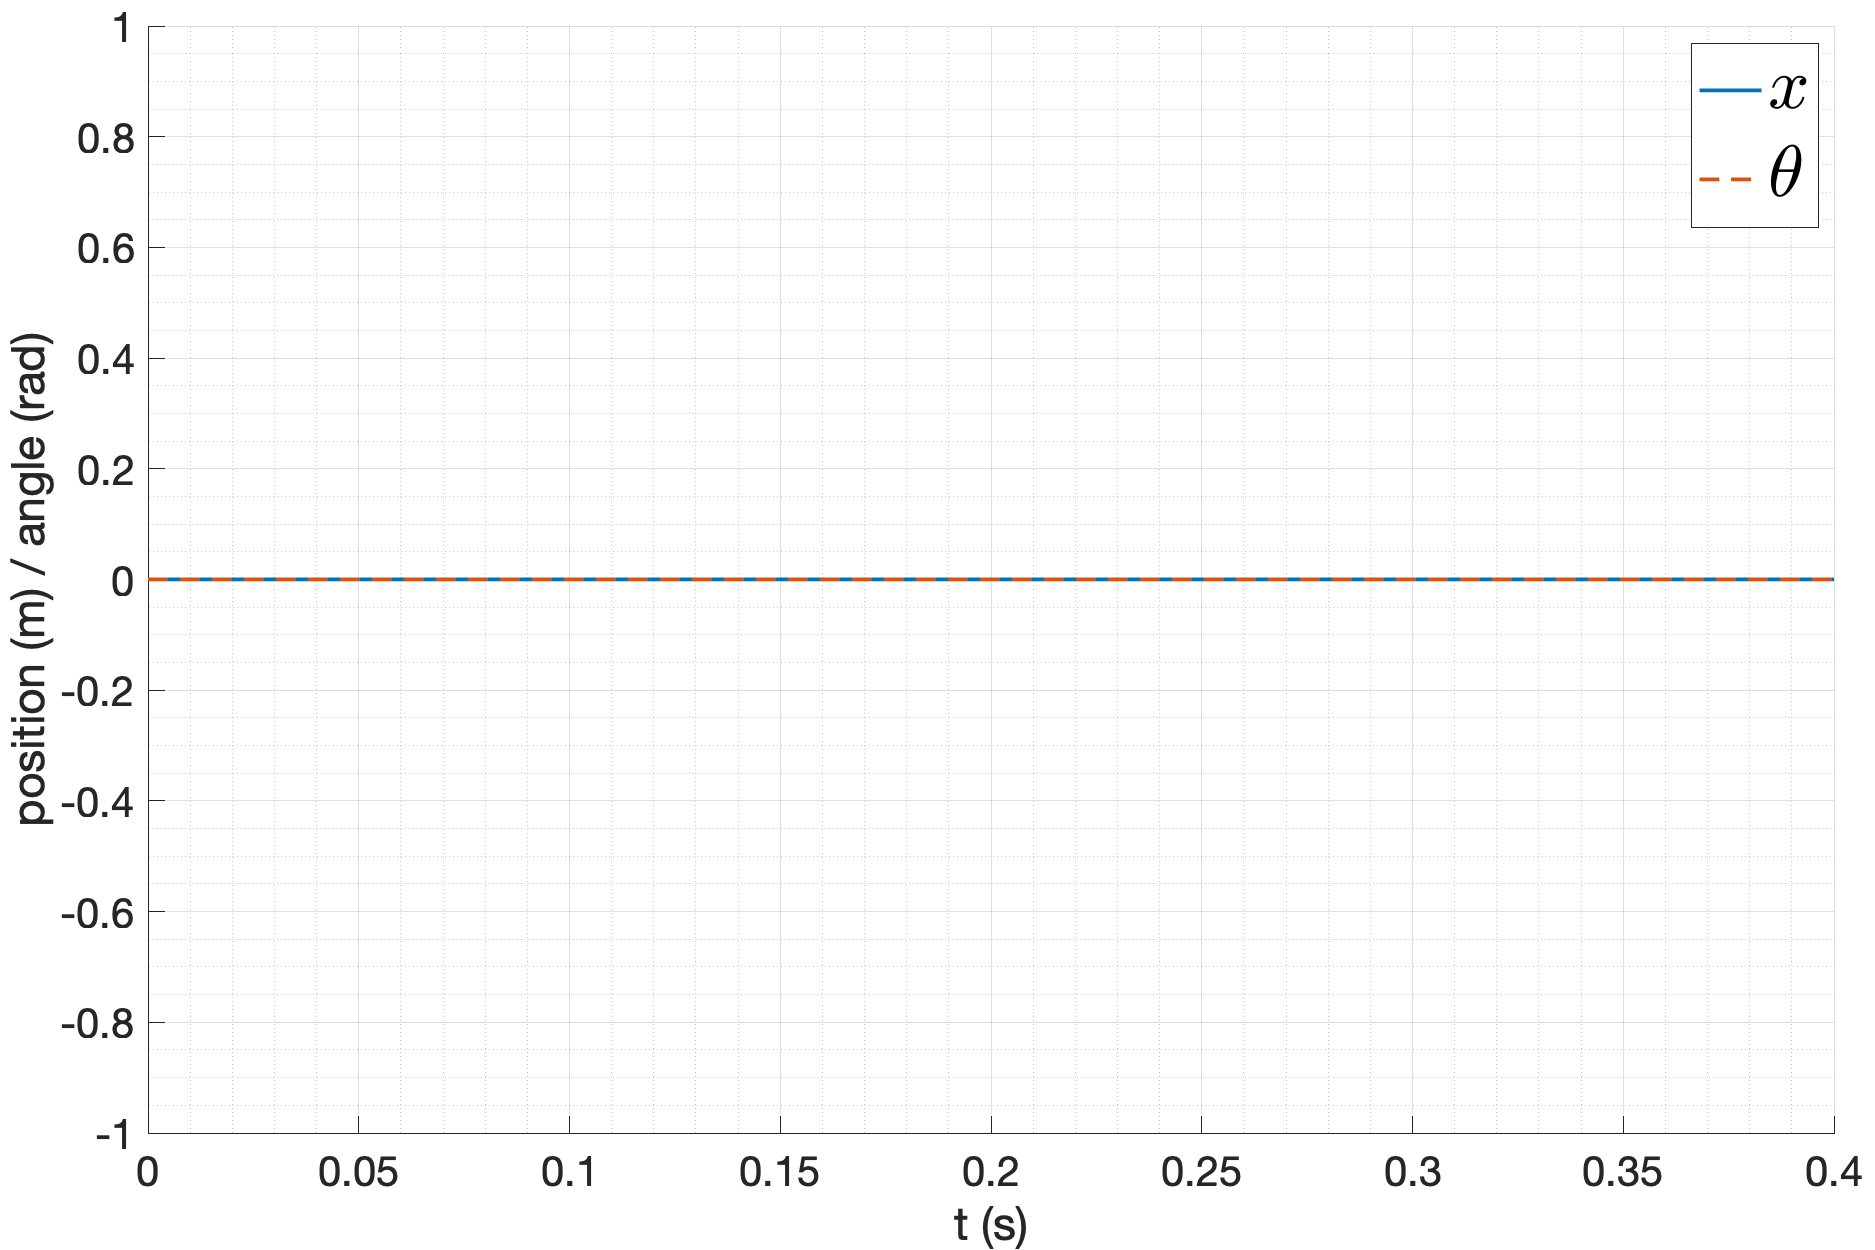
\includegraphics[width=\textwidth]{media/plots/free_motion/lin_1.png}
        \caption{$\theta_0 = 0$}
  \end{subfigure}
    \begin{subfigure}[b]{0.45\textwidth}
        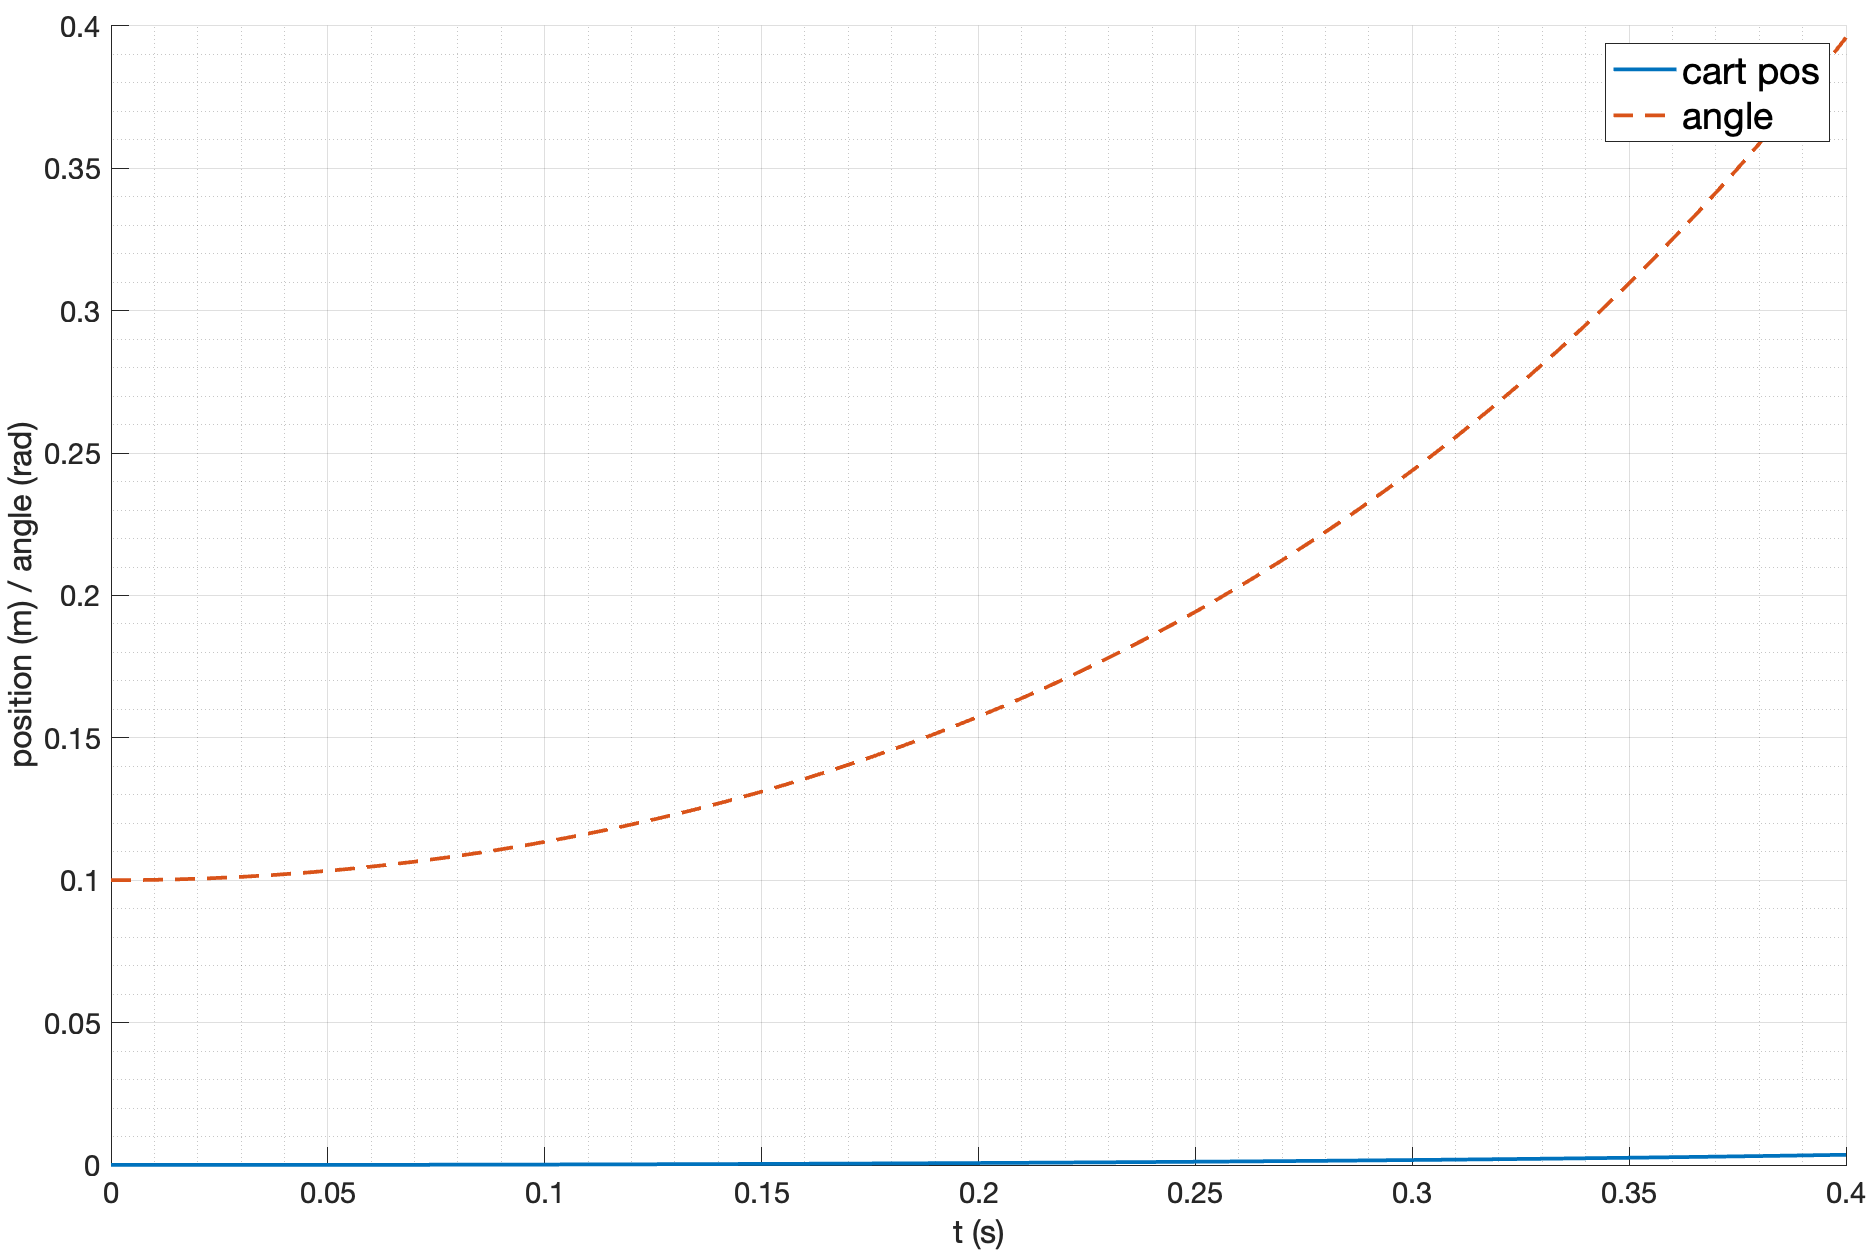
\includegraphics[width=\textwidth]{media/plots/free_motion/lin_2.png}
        \caption{$\theta_0 = 0.1$}
    \end{subfigure}
    \begin{subfigure}[b]{0.45\textwidth}
        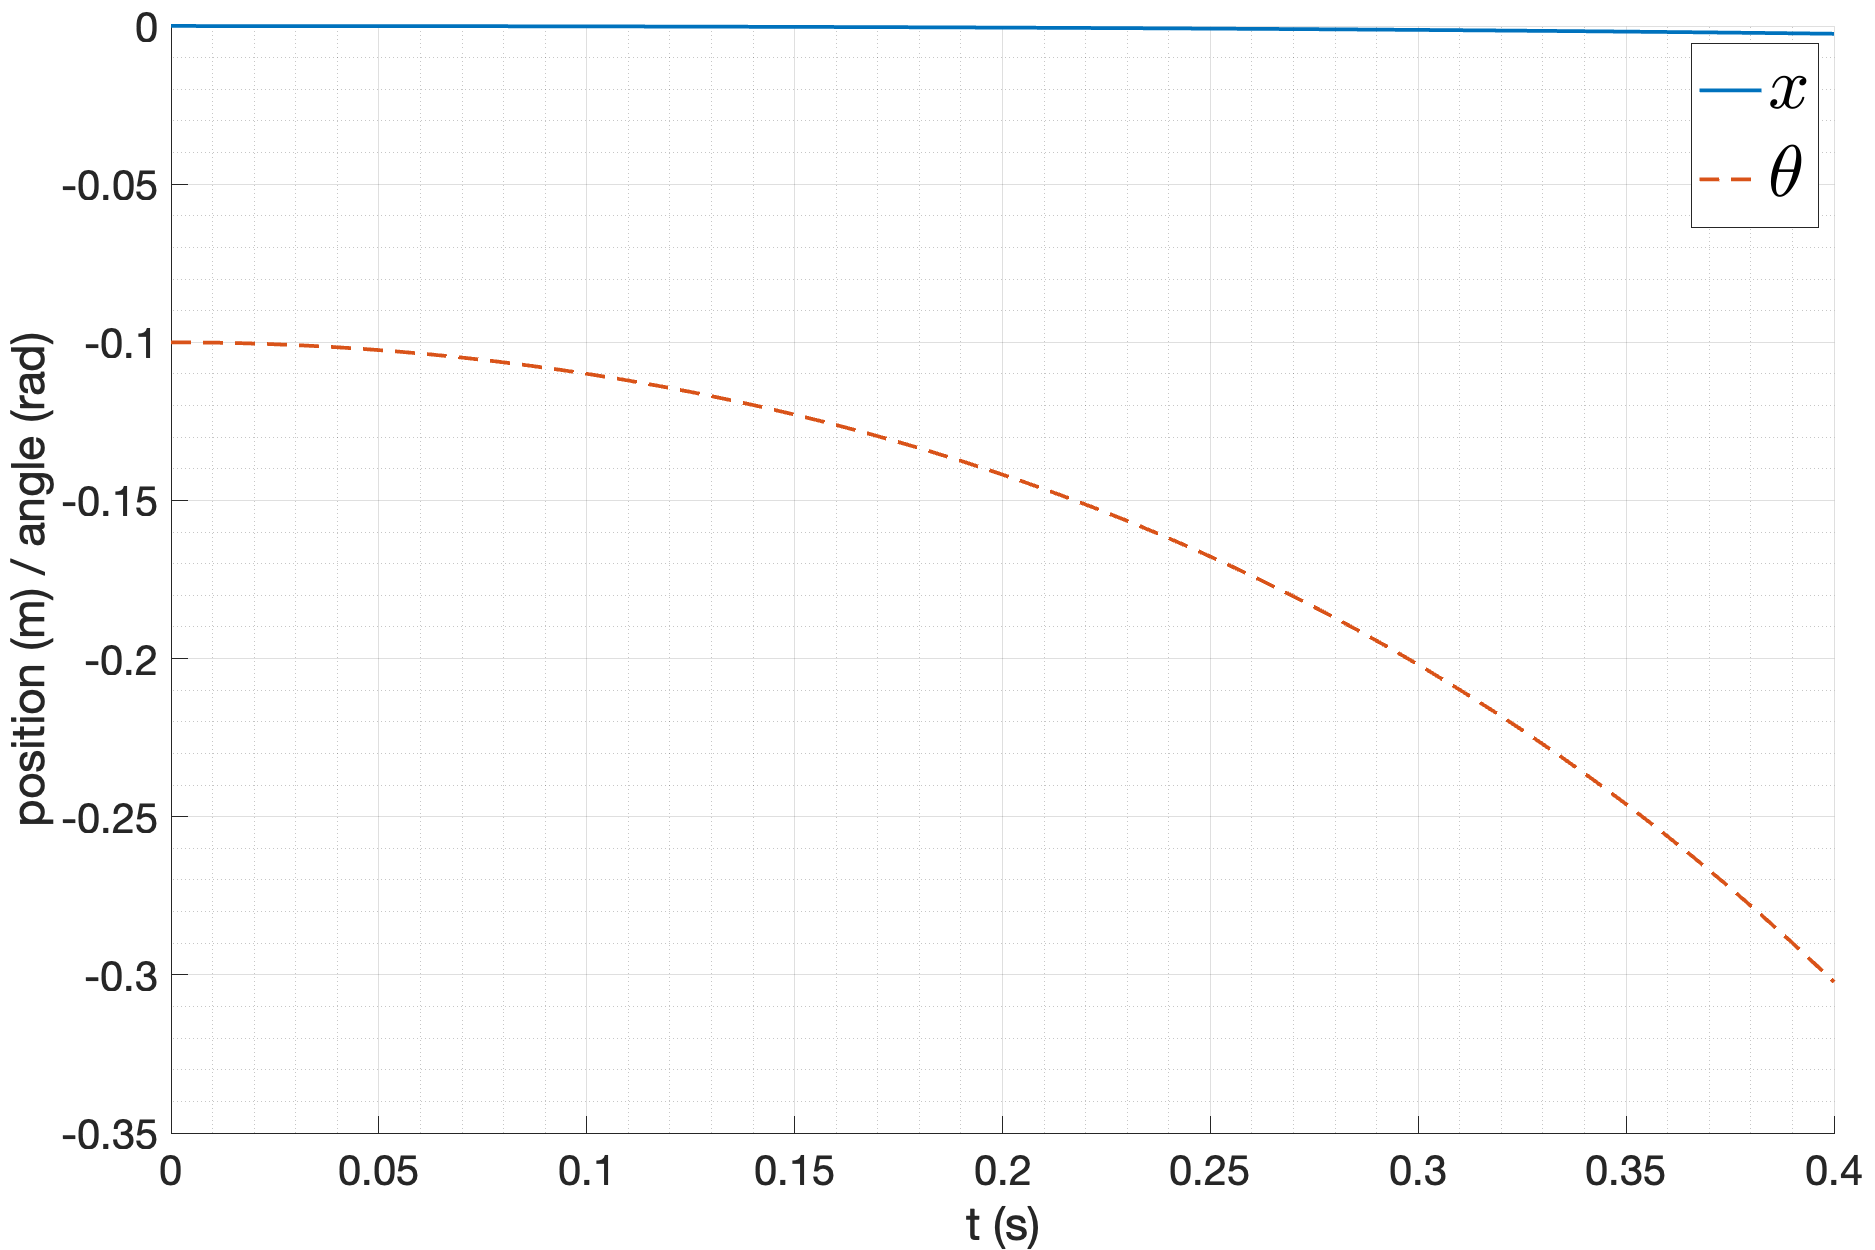
\includegraphics[width=\textwidth]{media/plots/free_motion/lin_3.png}
        \caption{$\theta_0 = -0.1$}
    \end{subfigure}
    \begin{subfigure}[b]{0.45\textwidth}
        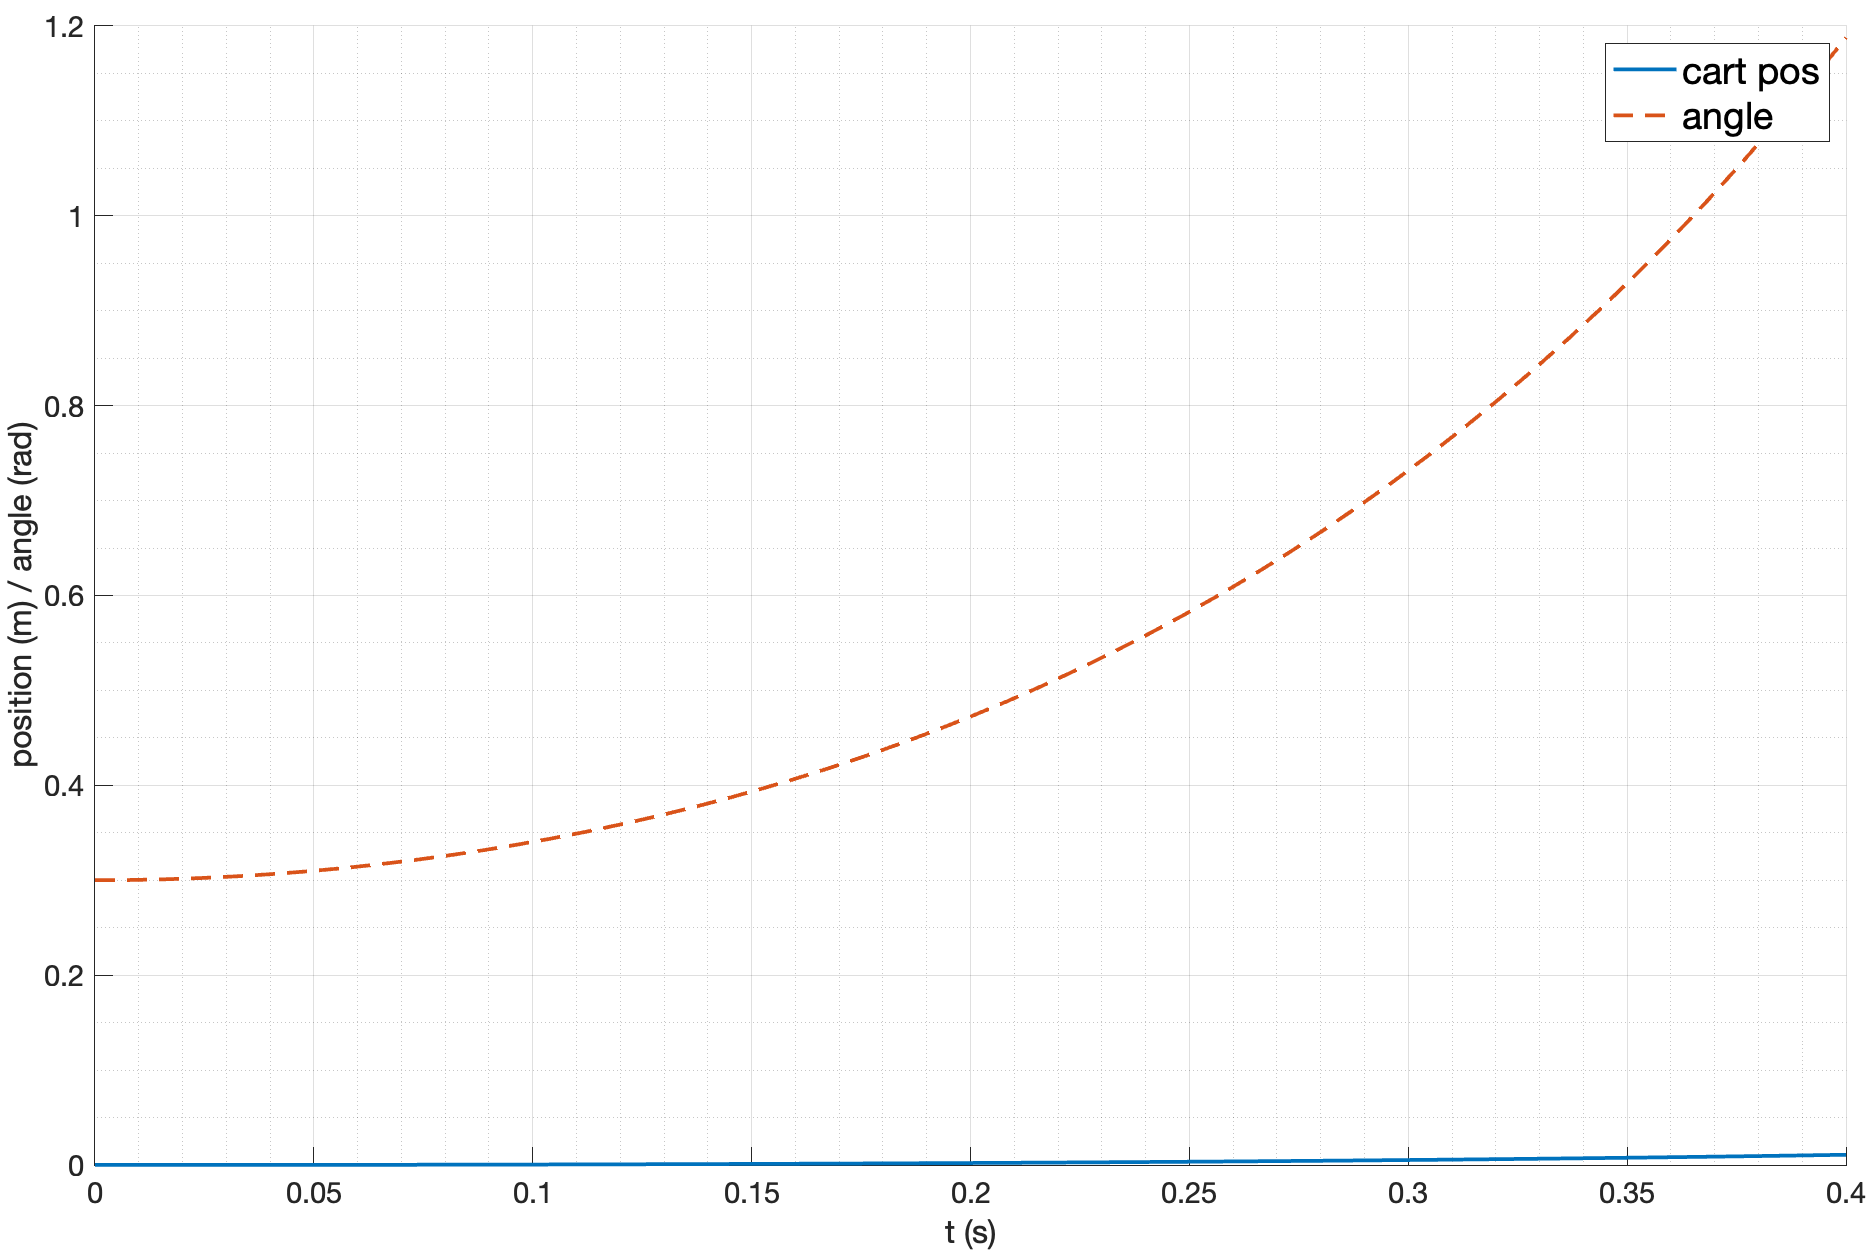
\includegraphics[width=\textwidth]{media/plots/free_motion/lin_4.png}
        \caption{$\theta_0 = 0.3$}
    \end{subfigure}
    \begin{subfigure}[b]{0.45\textwidth}
        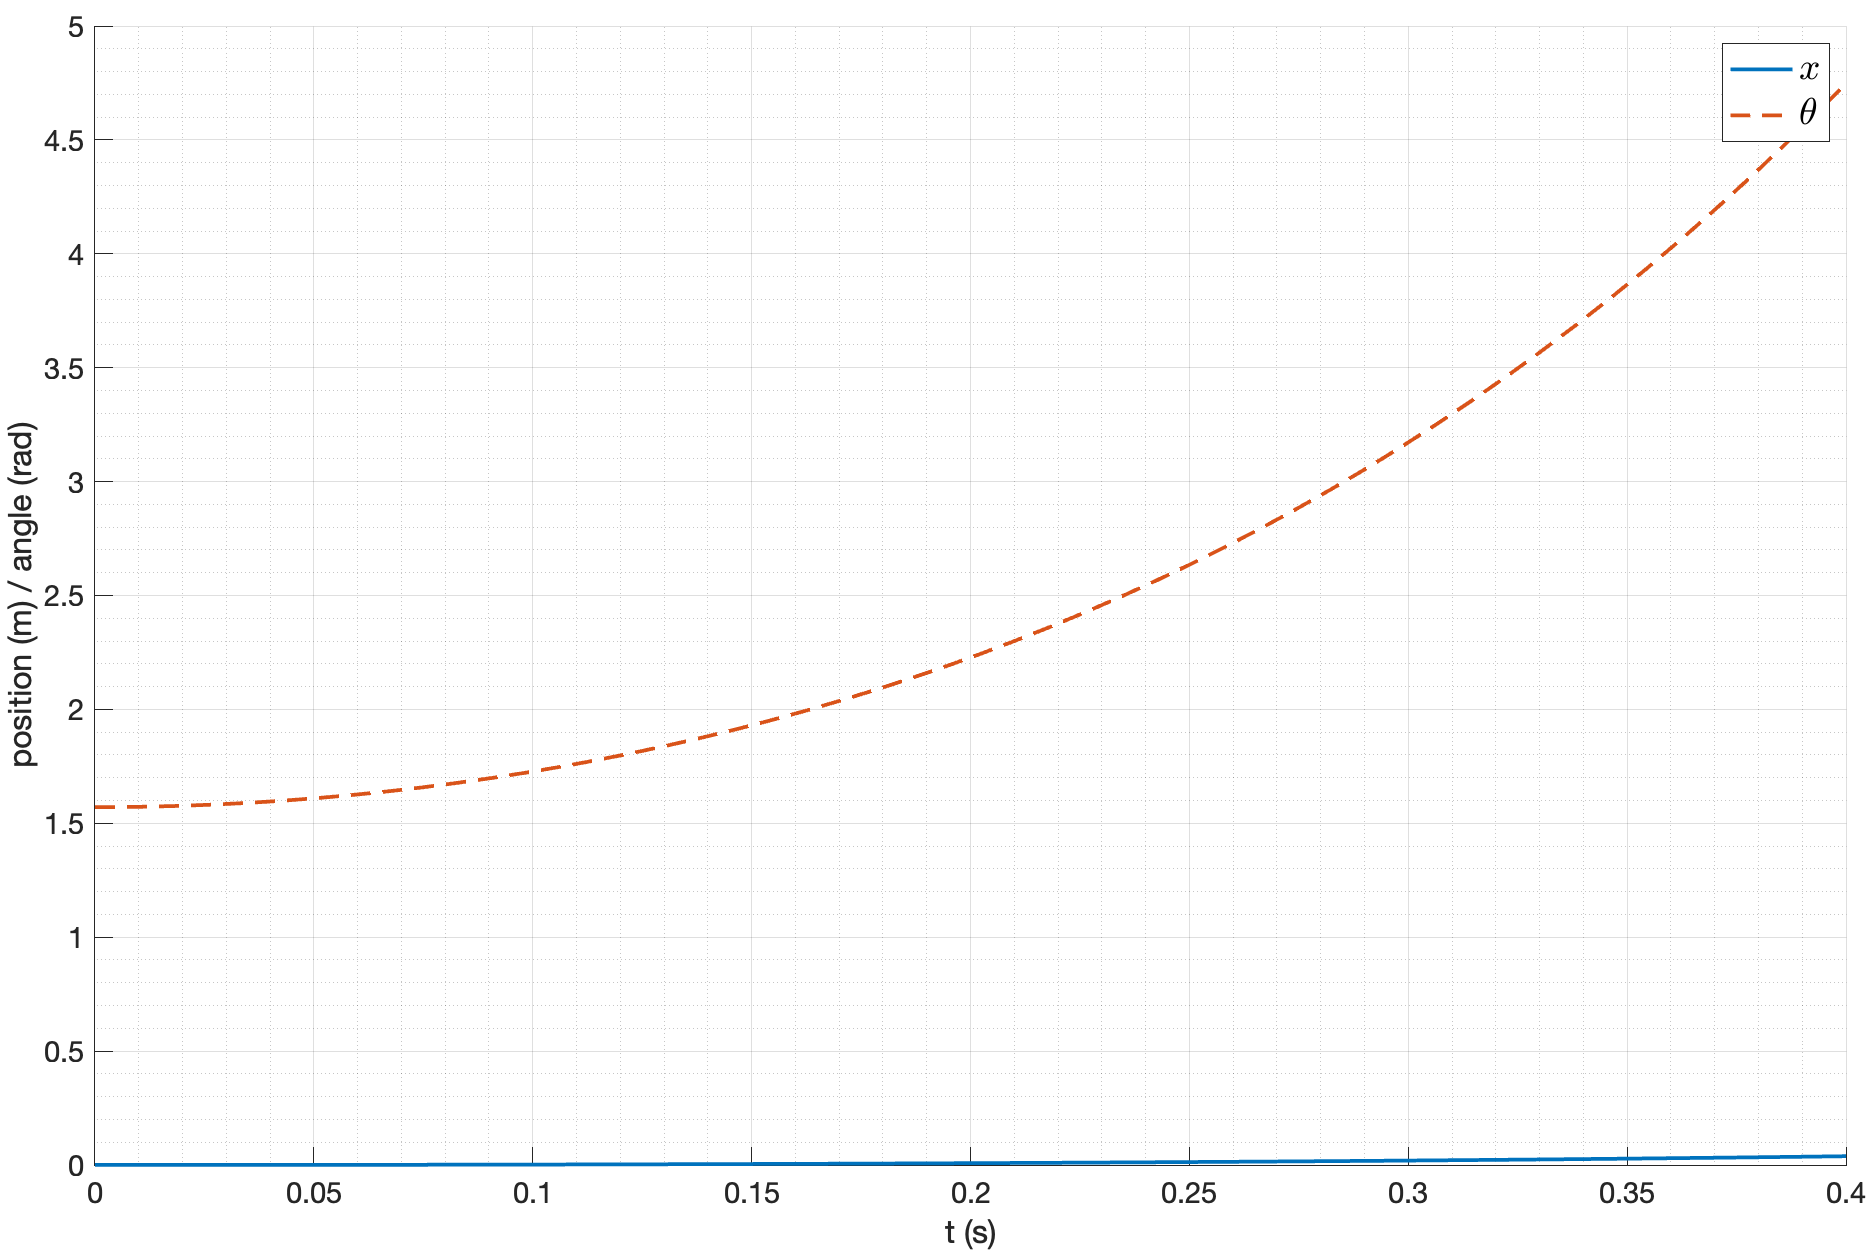
\includegraphics[width=\textwidth]{media/plots/free_motion/lin_5.png}
        \caption{$\theta_0 = \frac{\pi}{2}$}
    \end{subfigure}
    \begin{subfigure}[b]{0.45\textwidth}
        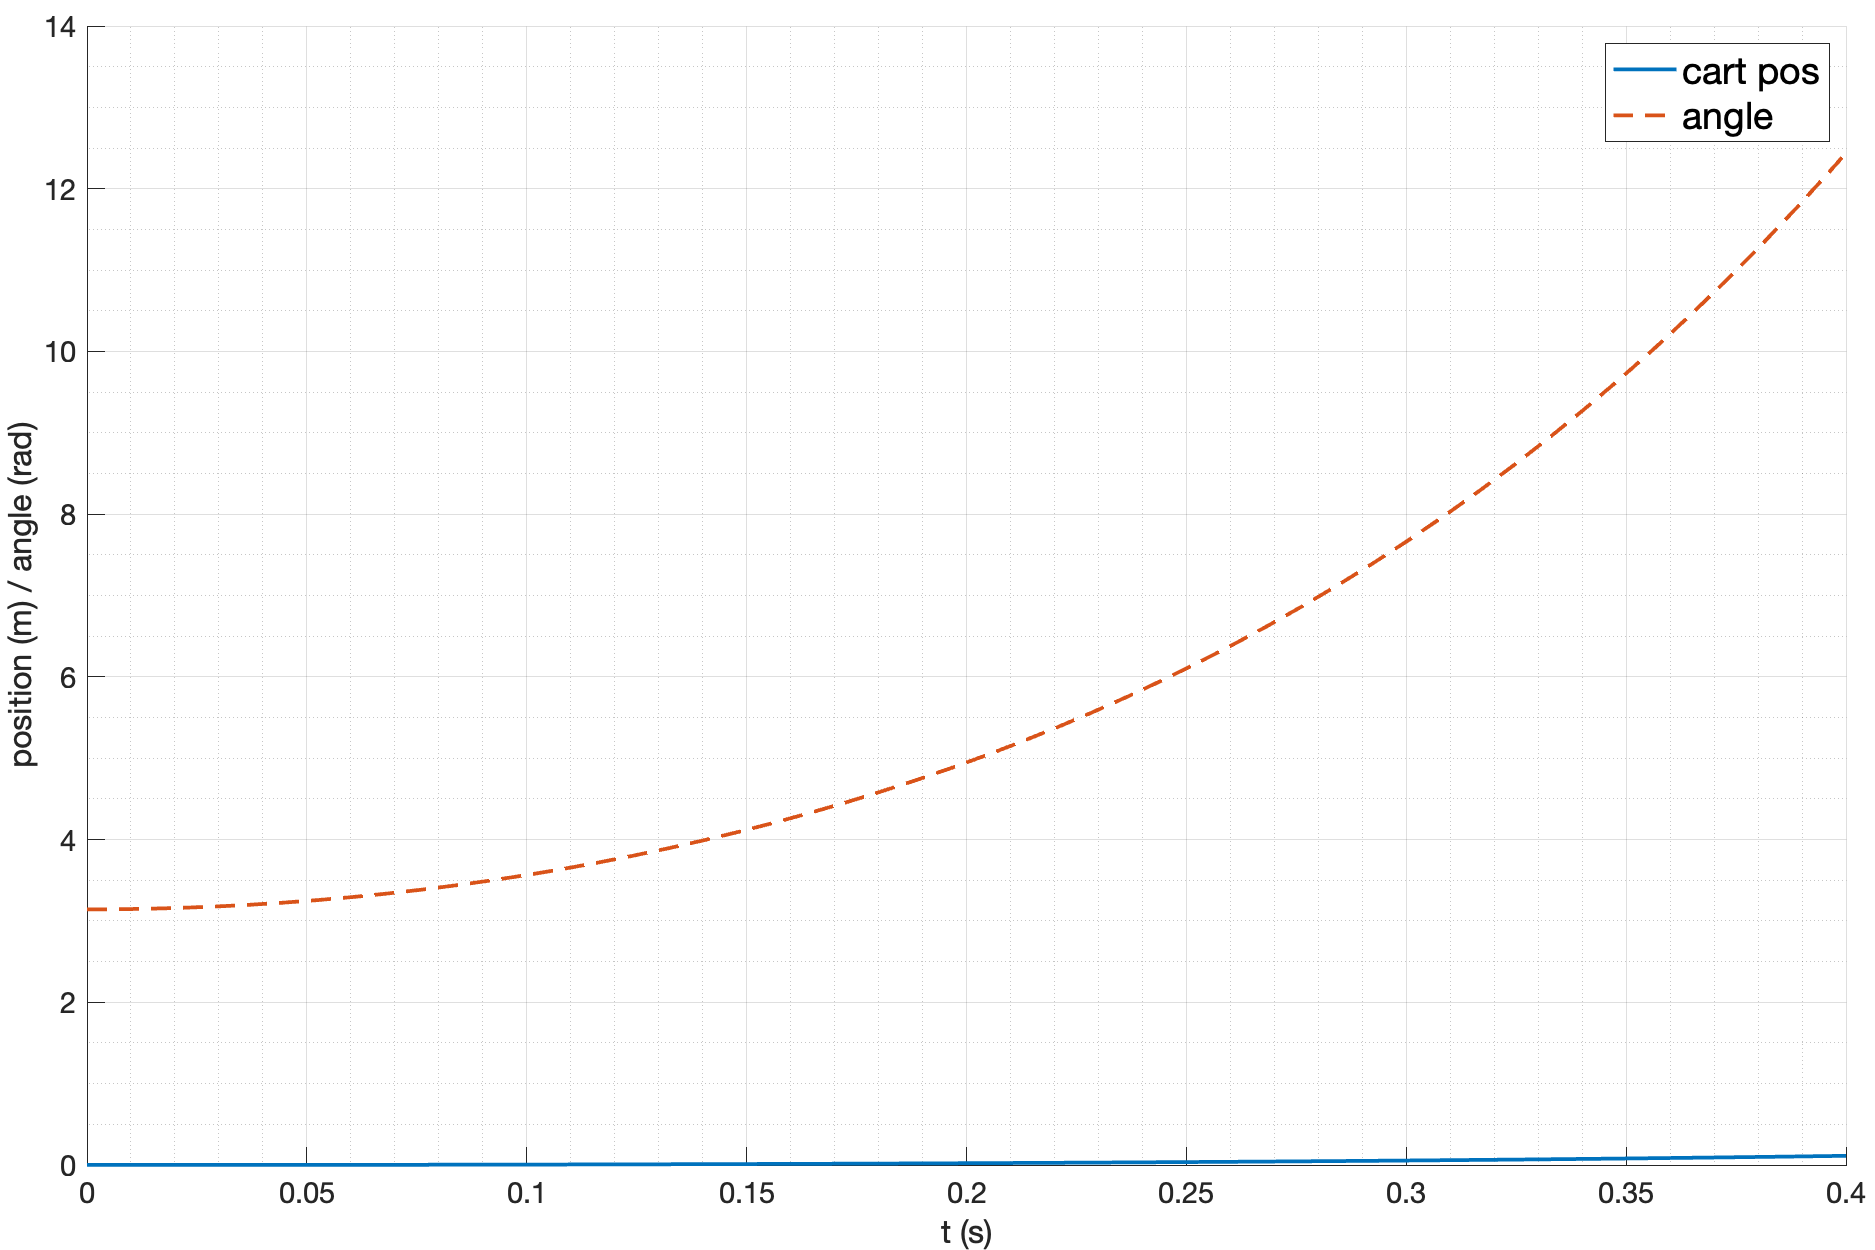
\includegraphics[width=\textwidth]{media/plots/free_motion/lin_6.png}
        \caption{$\theta_0 = \pi$}
    \end{subfigure}
    \caption{Свободное движение маятника (линеаризованная модель)}
    \label{fig:free_motion_linear}
\end{figure}

На рисунках \ref{fig:free_motion_nonlinear} и \ref{fig:free_motion_linear} видно, что при 
отсутствии отклонения от вертикального положения маятник остается в покое, 
при отклонении от вертикального положения маятник начинает движение, причем 
направление движения зависит от направления отклонения. При отклонении 
равным $\pi$, что соответствует нижнему положению равновесия, в случае нелинейной 
модели, остается неподвижным, в то время как в случае линеаризованной модели 
маятник начинает движение, что связано с тем, что линеаризация проводилась в окрестности
верхней точки равновесия, а не нижней. Сравним результаты моделирования
нелинейной и линеаризованной моделей. Графики различия движения приведены на
рисунке \ref{fig:free_motion_err}. 

\begin{figure}[ht!]
    \centering
    \begin{subfigure}[b]{0.45\textwidth}
        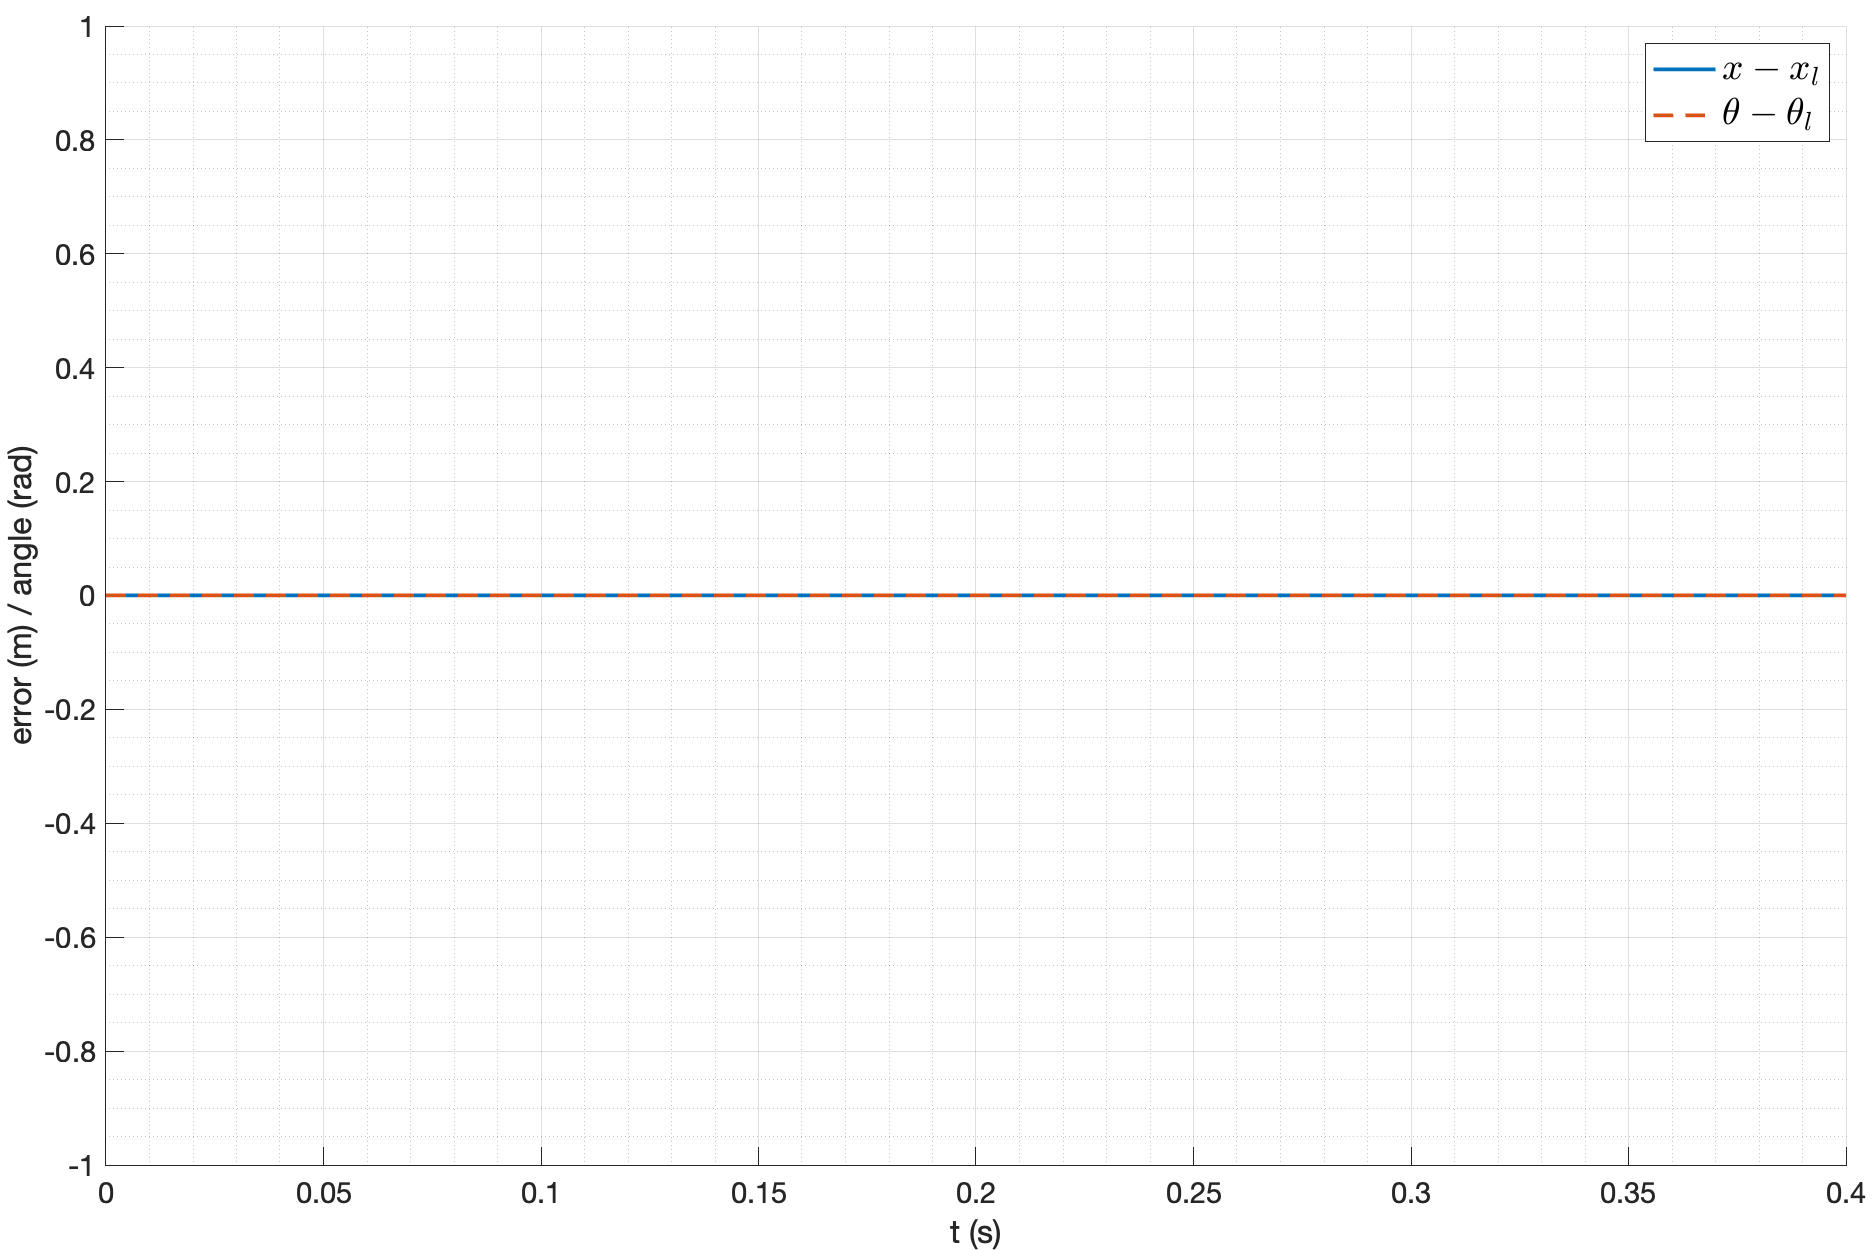
\includegraphics[width=\textwidth]{media/plots/free_motion/err_1.png}
        \caption{$\theta_0 = 0$}
  \end{subfigure}
    \begin{subfigure}[b]{0.45\textwidth}
        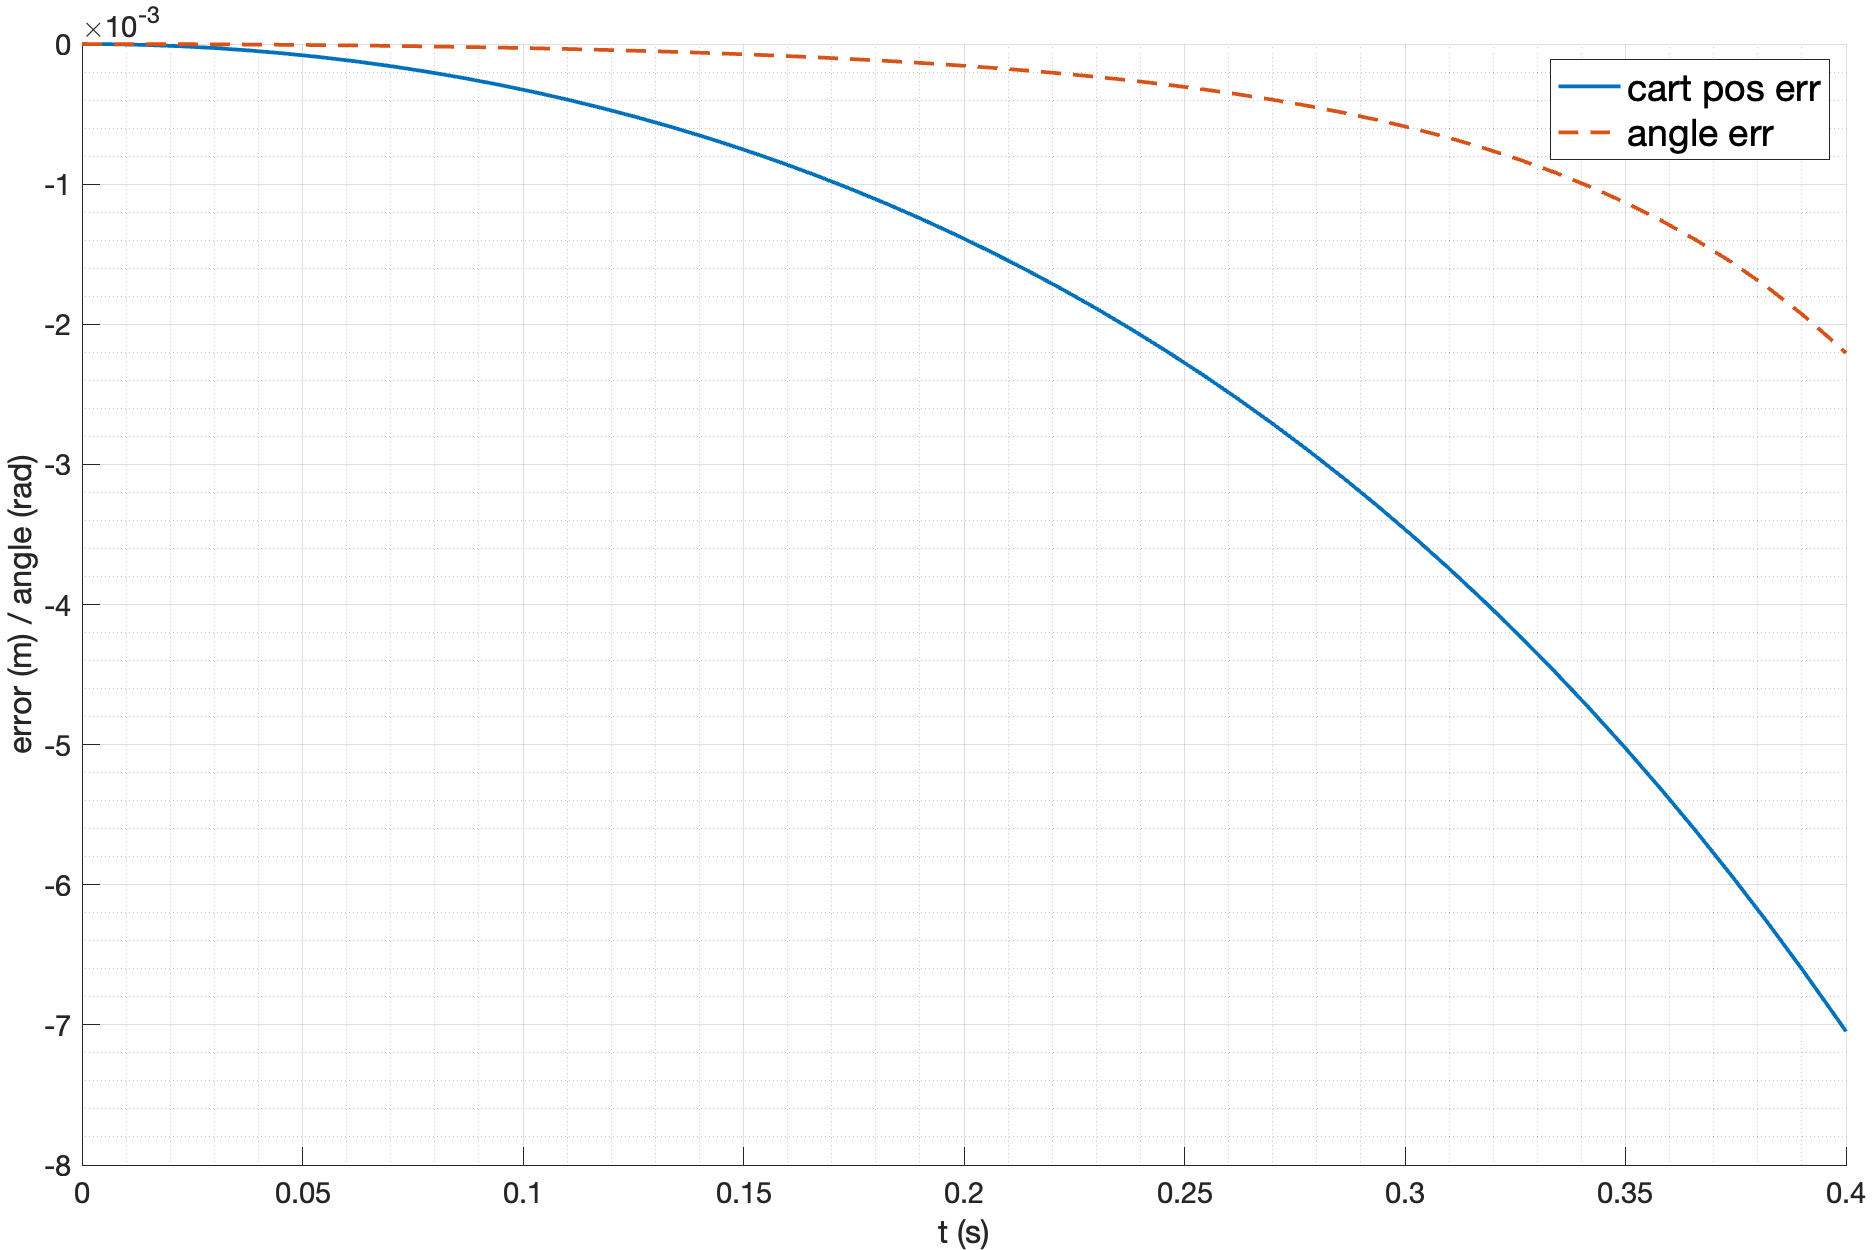
\includegraphics[width=\textwidth]{media/plots/free_motion/err_2.png}
        \caption{$\theta_0 = 0.1$}
    \end{subfigure}
    \begin{subfigure}[b]{0.45\textwidth}
        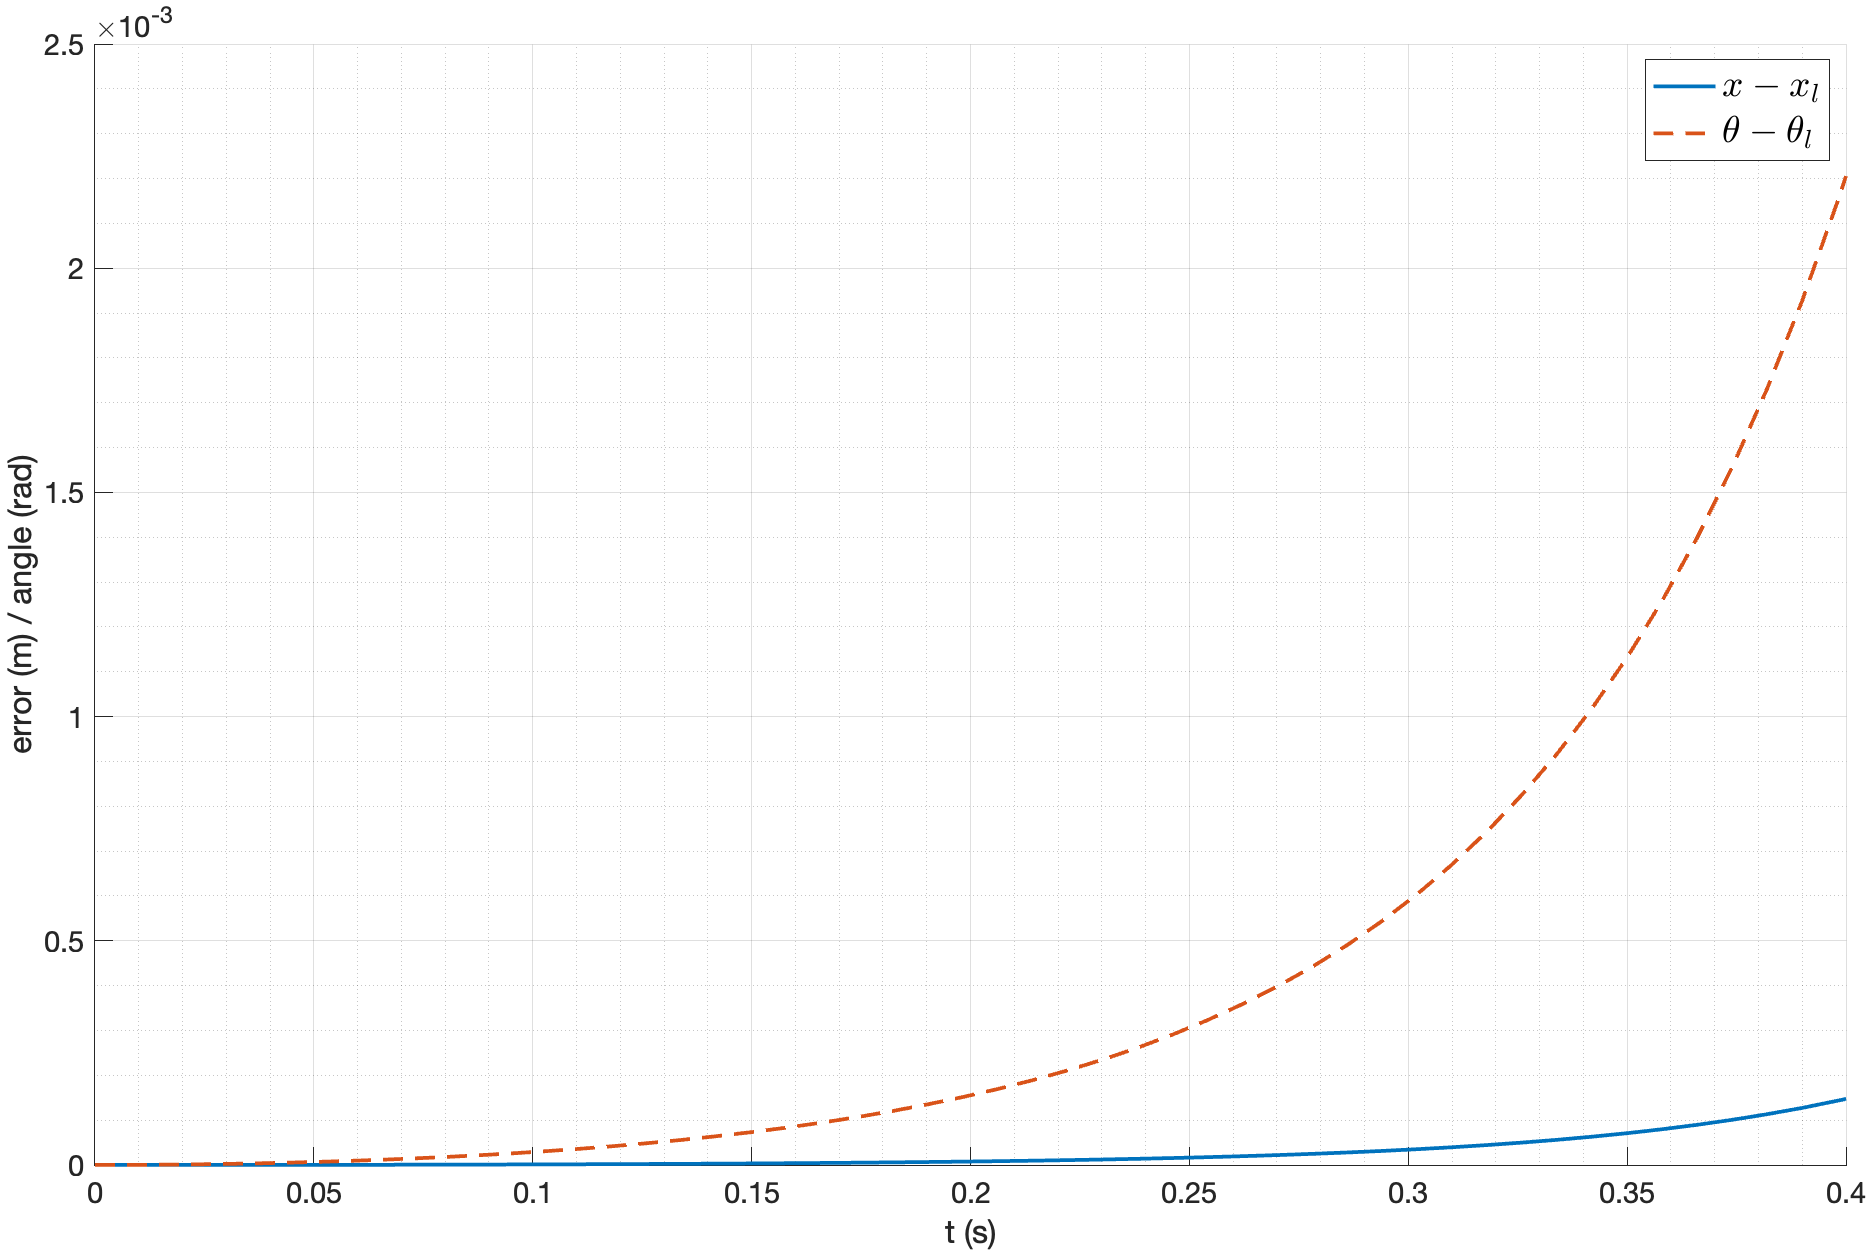
\includegraphics[width=\textwidth]{media/plots/free_motion/err_3.png}
        \caption{$\theta_0 = -0.1$}
    \end{subfigure}
    \begin{subfigure}[b]{0.45\textwidth}
        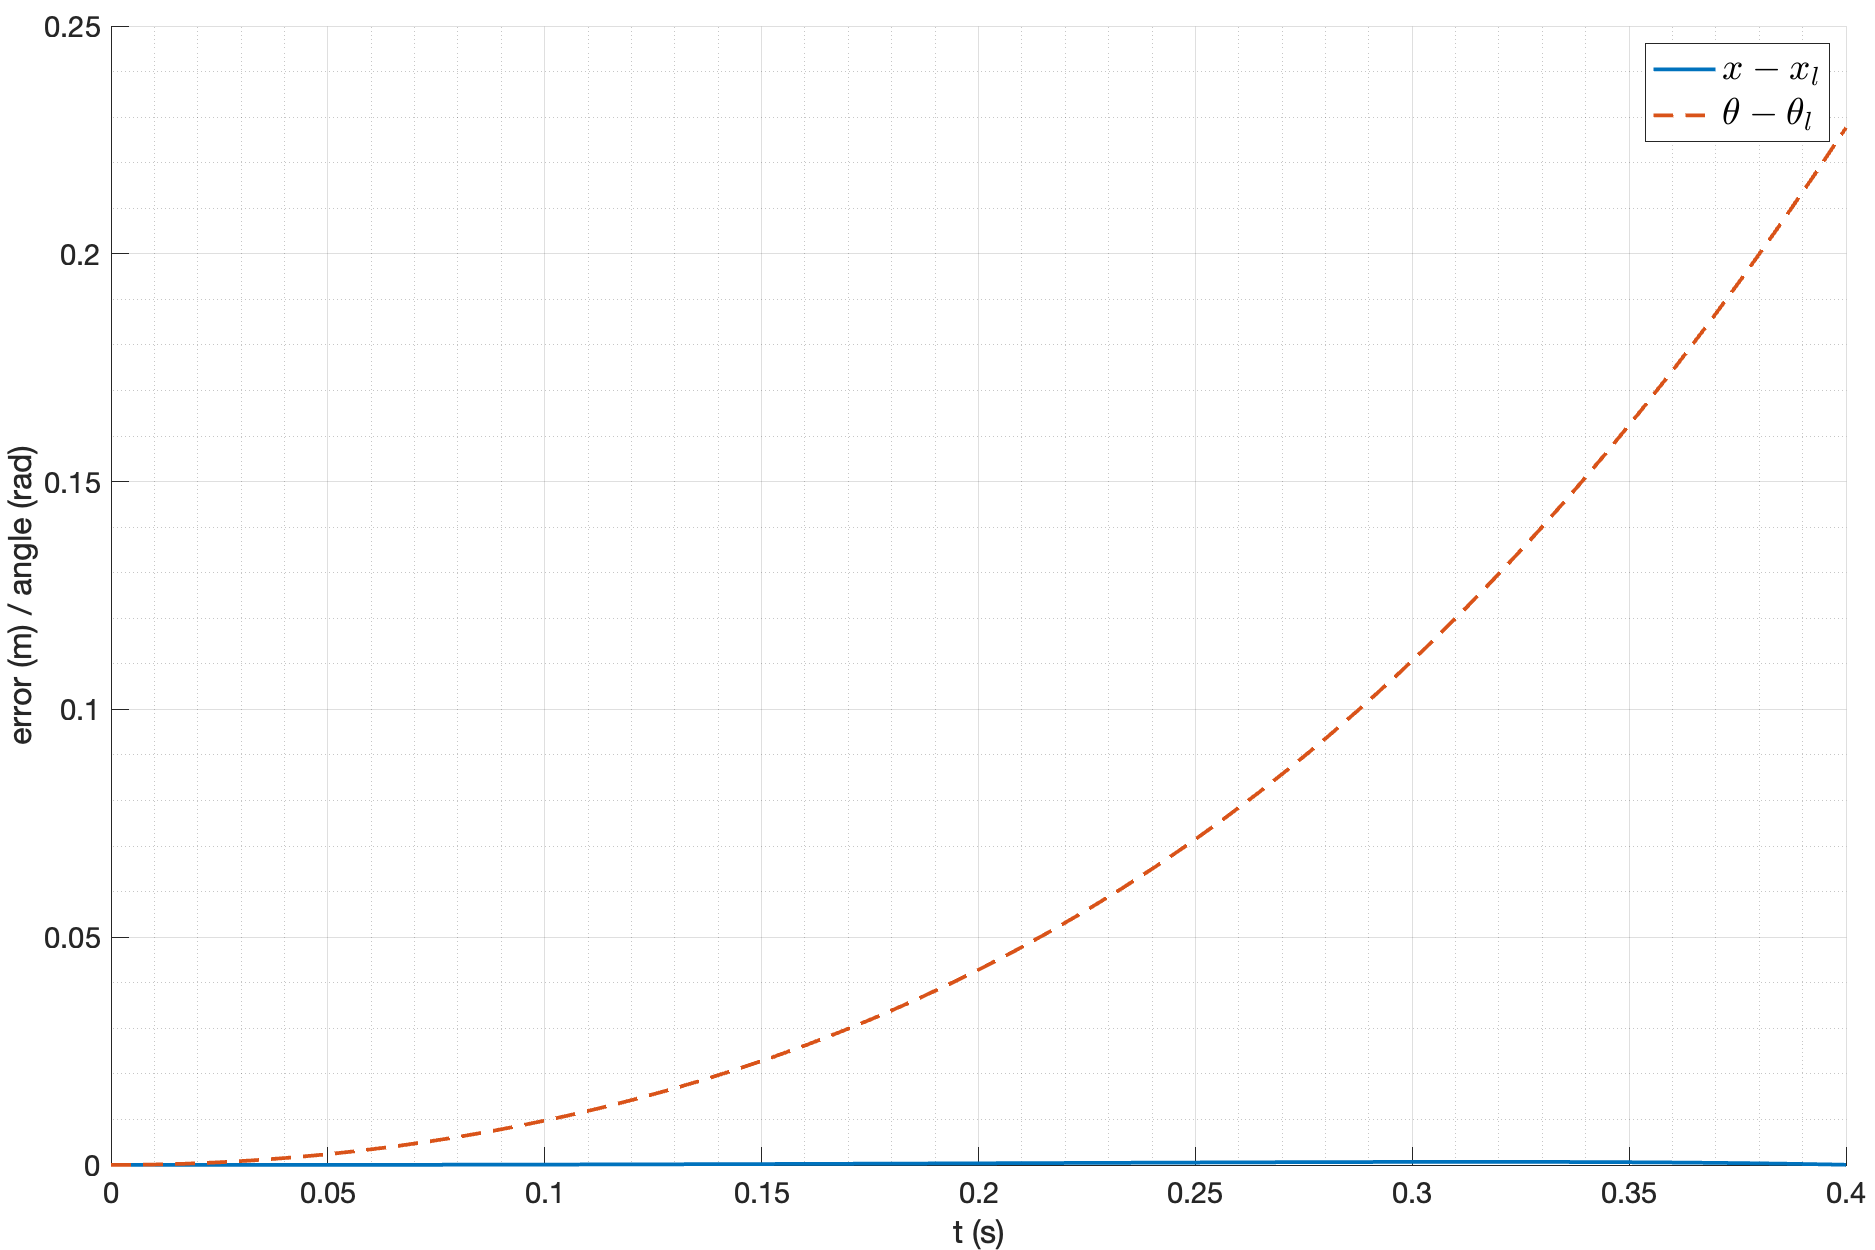
\includegraphics[width=\textwidth]{media/plots/free_motion/err_4.png}
        \caption{$\theta_0 = 0.3$}
    \end{subfigure}
    \begin{subfigure}[b]{0.45\textwidth}
        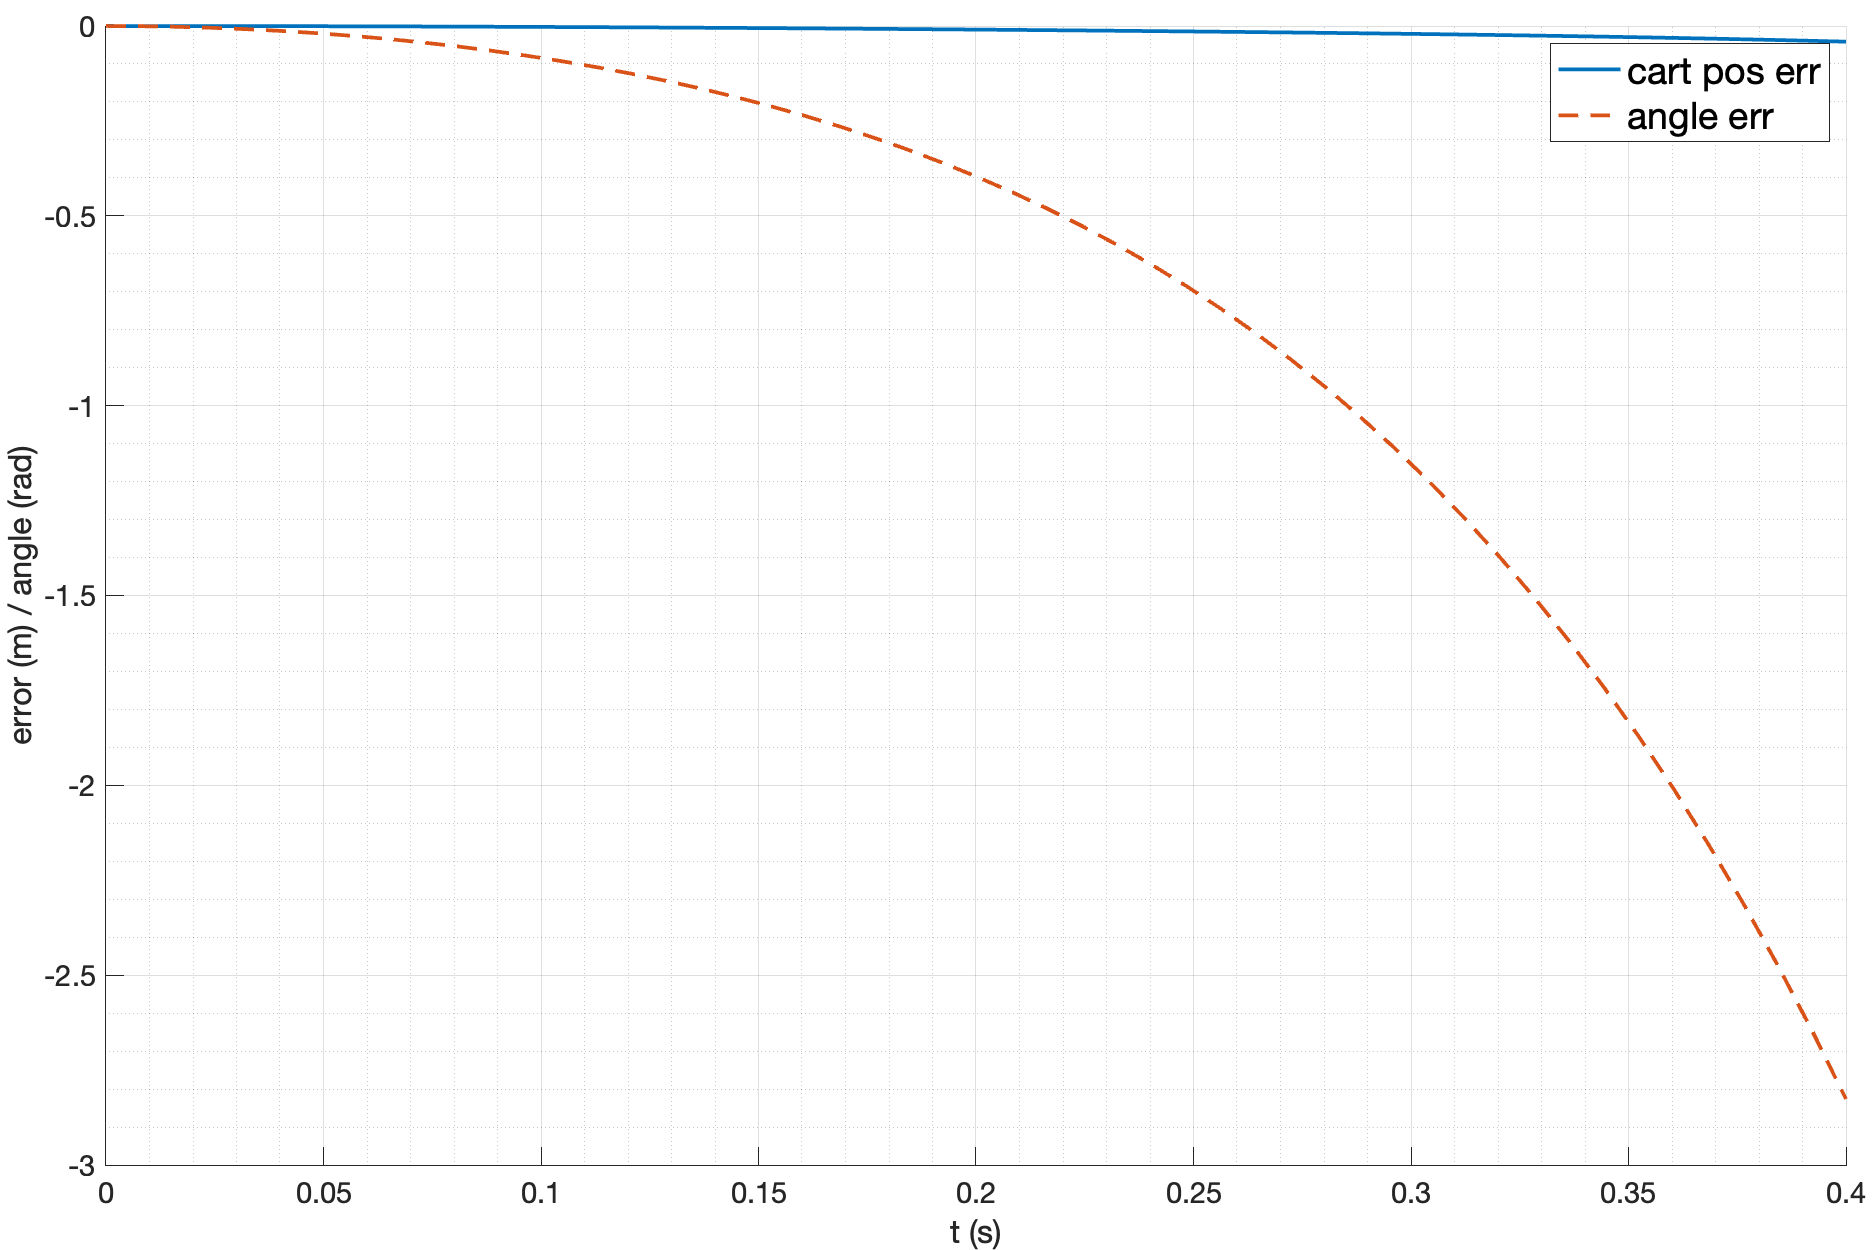
\includegraphics[width=\textwidth]{media/plots/free_motion/err_5.png}
        \caption{$\theta_0 = \frac{\pi}{2}$}
    \end{subfigure}
    \begin{subfigure}[b]{0.45\textwidth}
        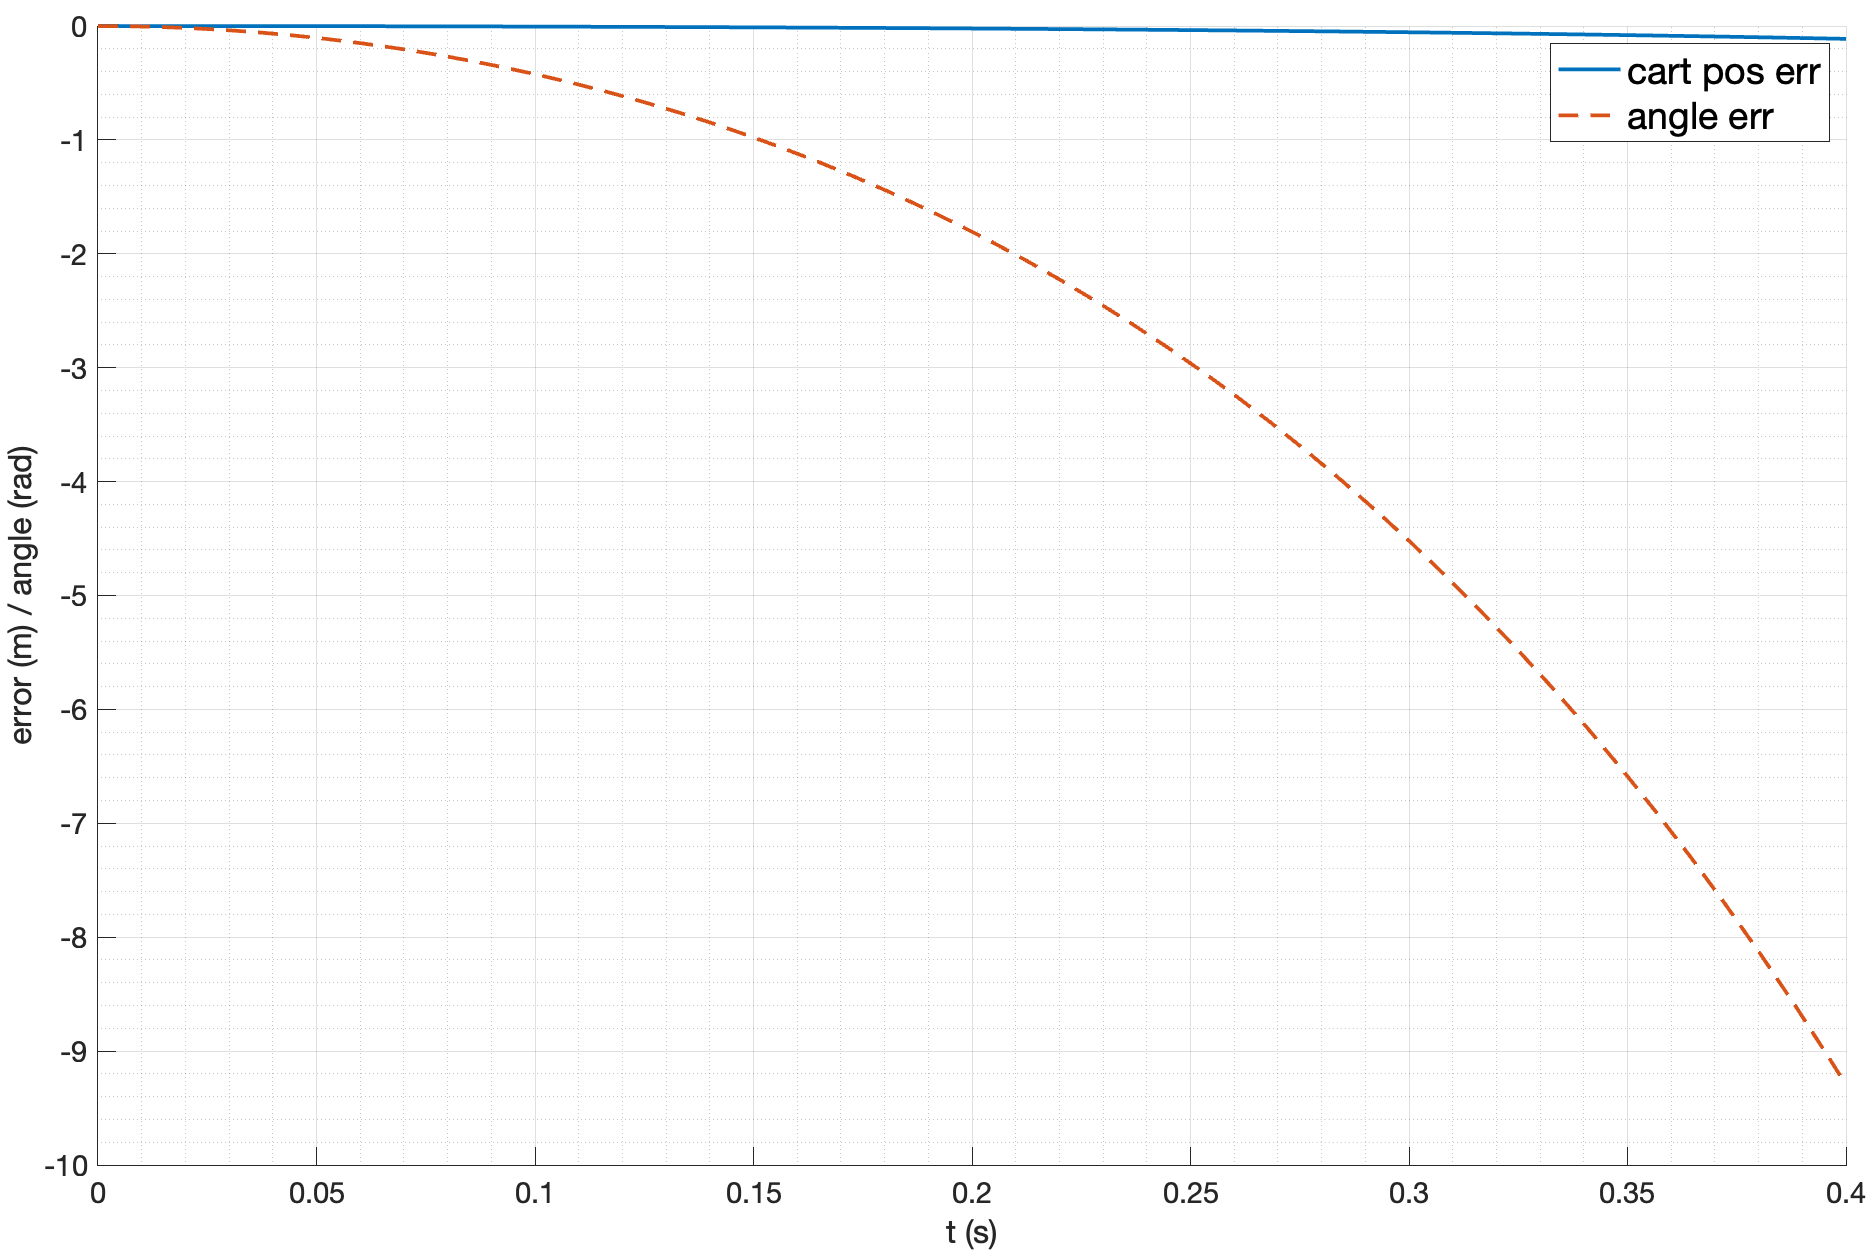
\includegraphics[width=\textwidth]{media/plots/free_motion/err_6.png}
        \caption{$\theta_0 = \pi$}
    \end{subfigure}
    \caption{Различия в движении маятника (нелинейная и линеаризованная модели)}
    \label{fig:free_motion_err}
\end{figure}

Видно, что при отклонениях $\theta_0 = 0.1$, $\theta_0 = -0.1$ и $\theta_0 = 0.3$ 
различия в движении незначительны, при этом увеличиваются с увеличением 
модуля отклонения. При отклонении $\theta_0 = \frac{\pi}{2}$ различия в движении
уже становятся существенными, что, опять же, связано с линеаризацией вблизи 
верхней точки равновесия. 

Проведем моделирование системы с начальным отклонением $\theta_0 = 0.1$ на более длительном 
промежутке времени. Результаты моделирования представлены на рисунке \ref{fig:free_motion_long_linear}, 
\ref{fig:free_motion_long_nonlinear}. 
\begin{figure}[ht!]
    \centering
    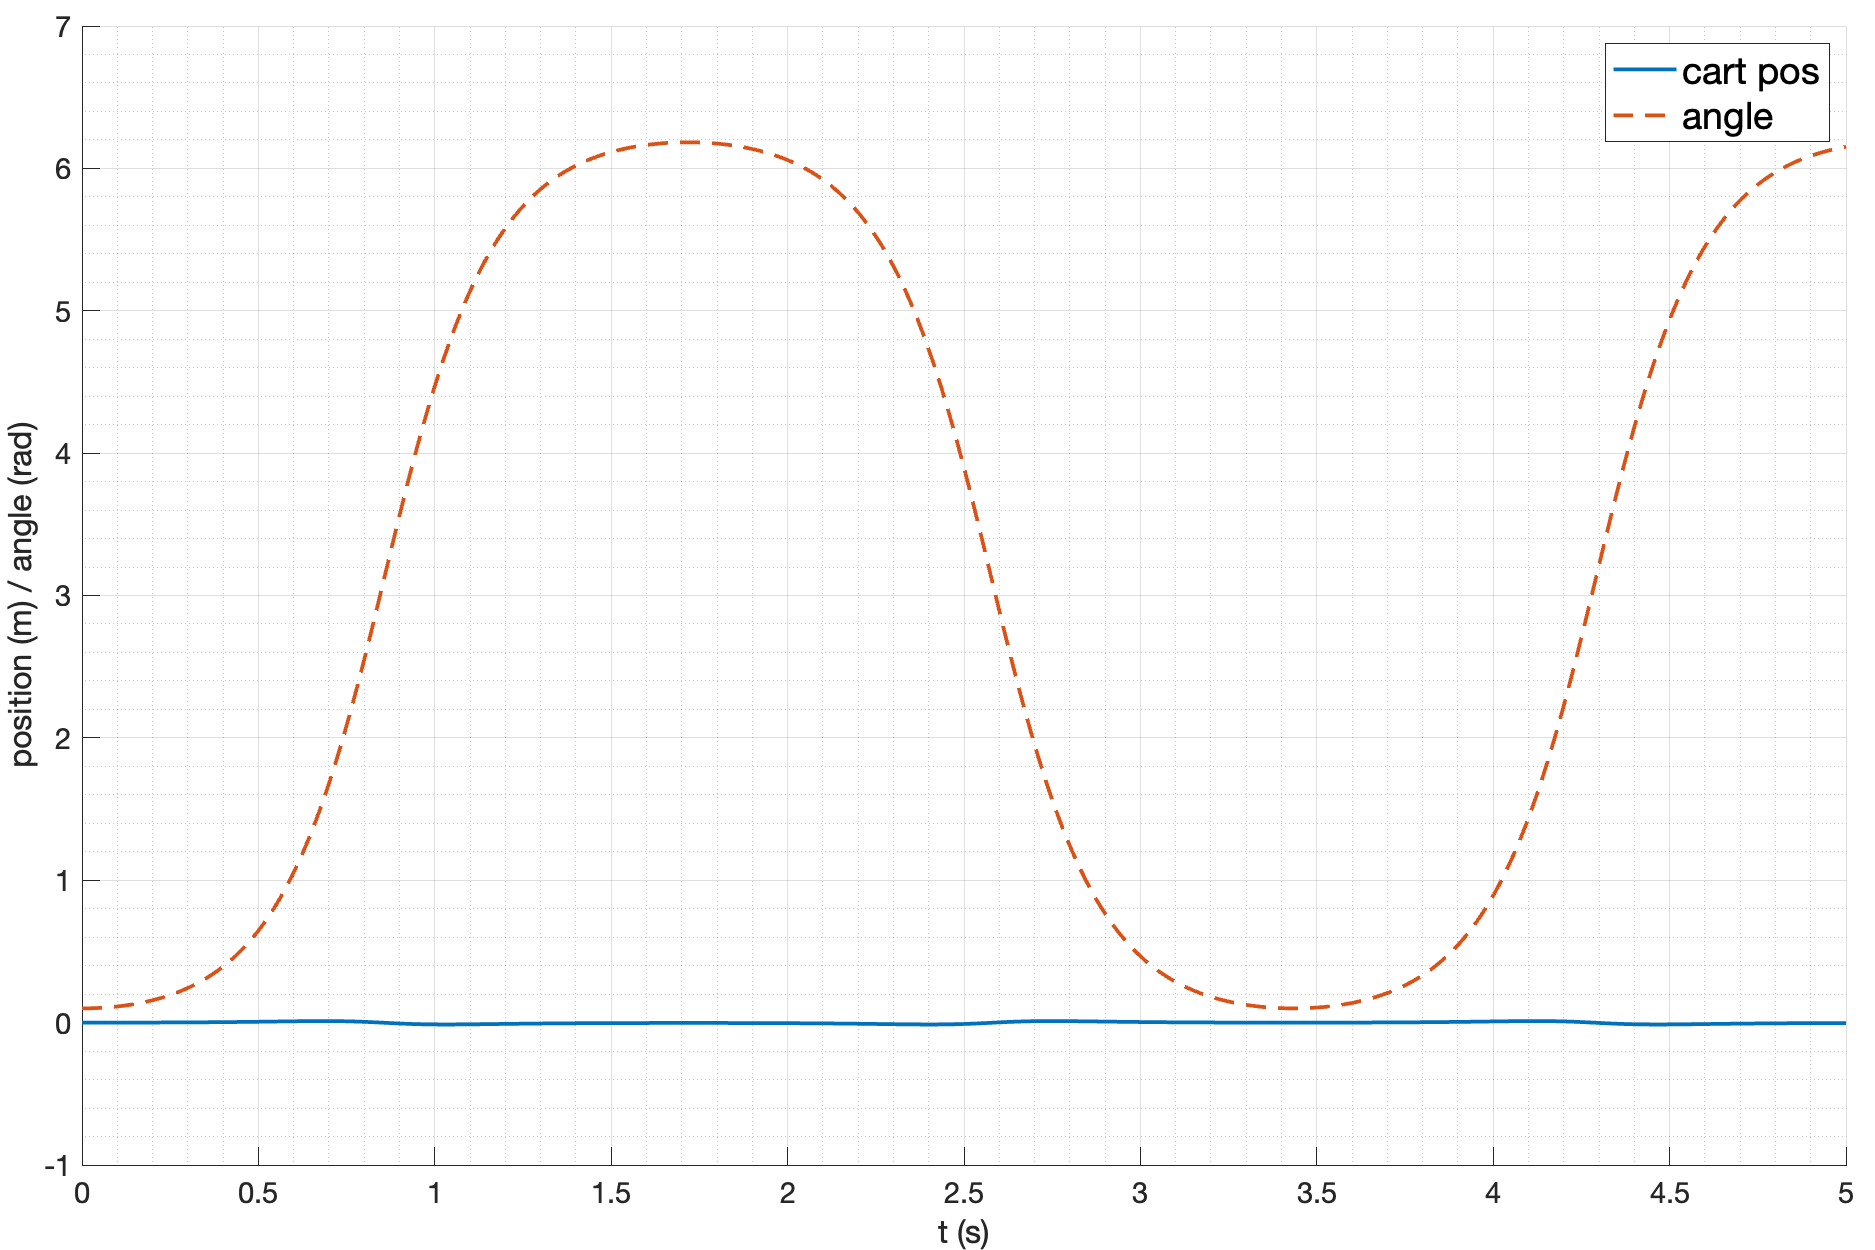
\includegraphics[width=\textwidth]{media/plots/free_motion/long.png}
    \caption{Свободное движение маятника (нелинейная модель)}
    \label{fig:free_motion_long_nonlinear}
\end{figure}
\begin{figure}[ht!]
    \centering
    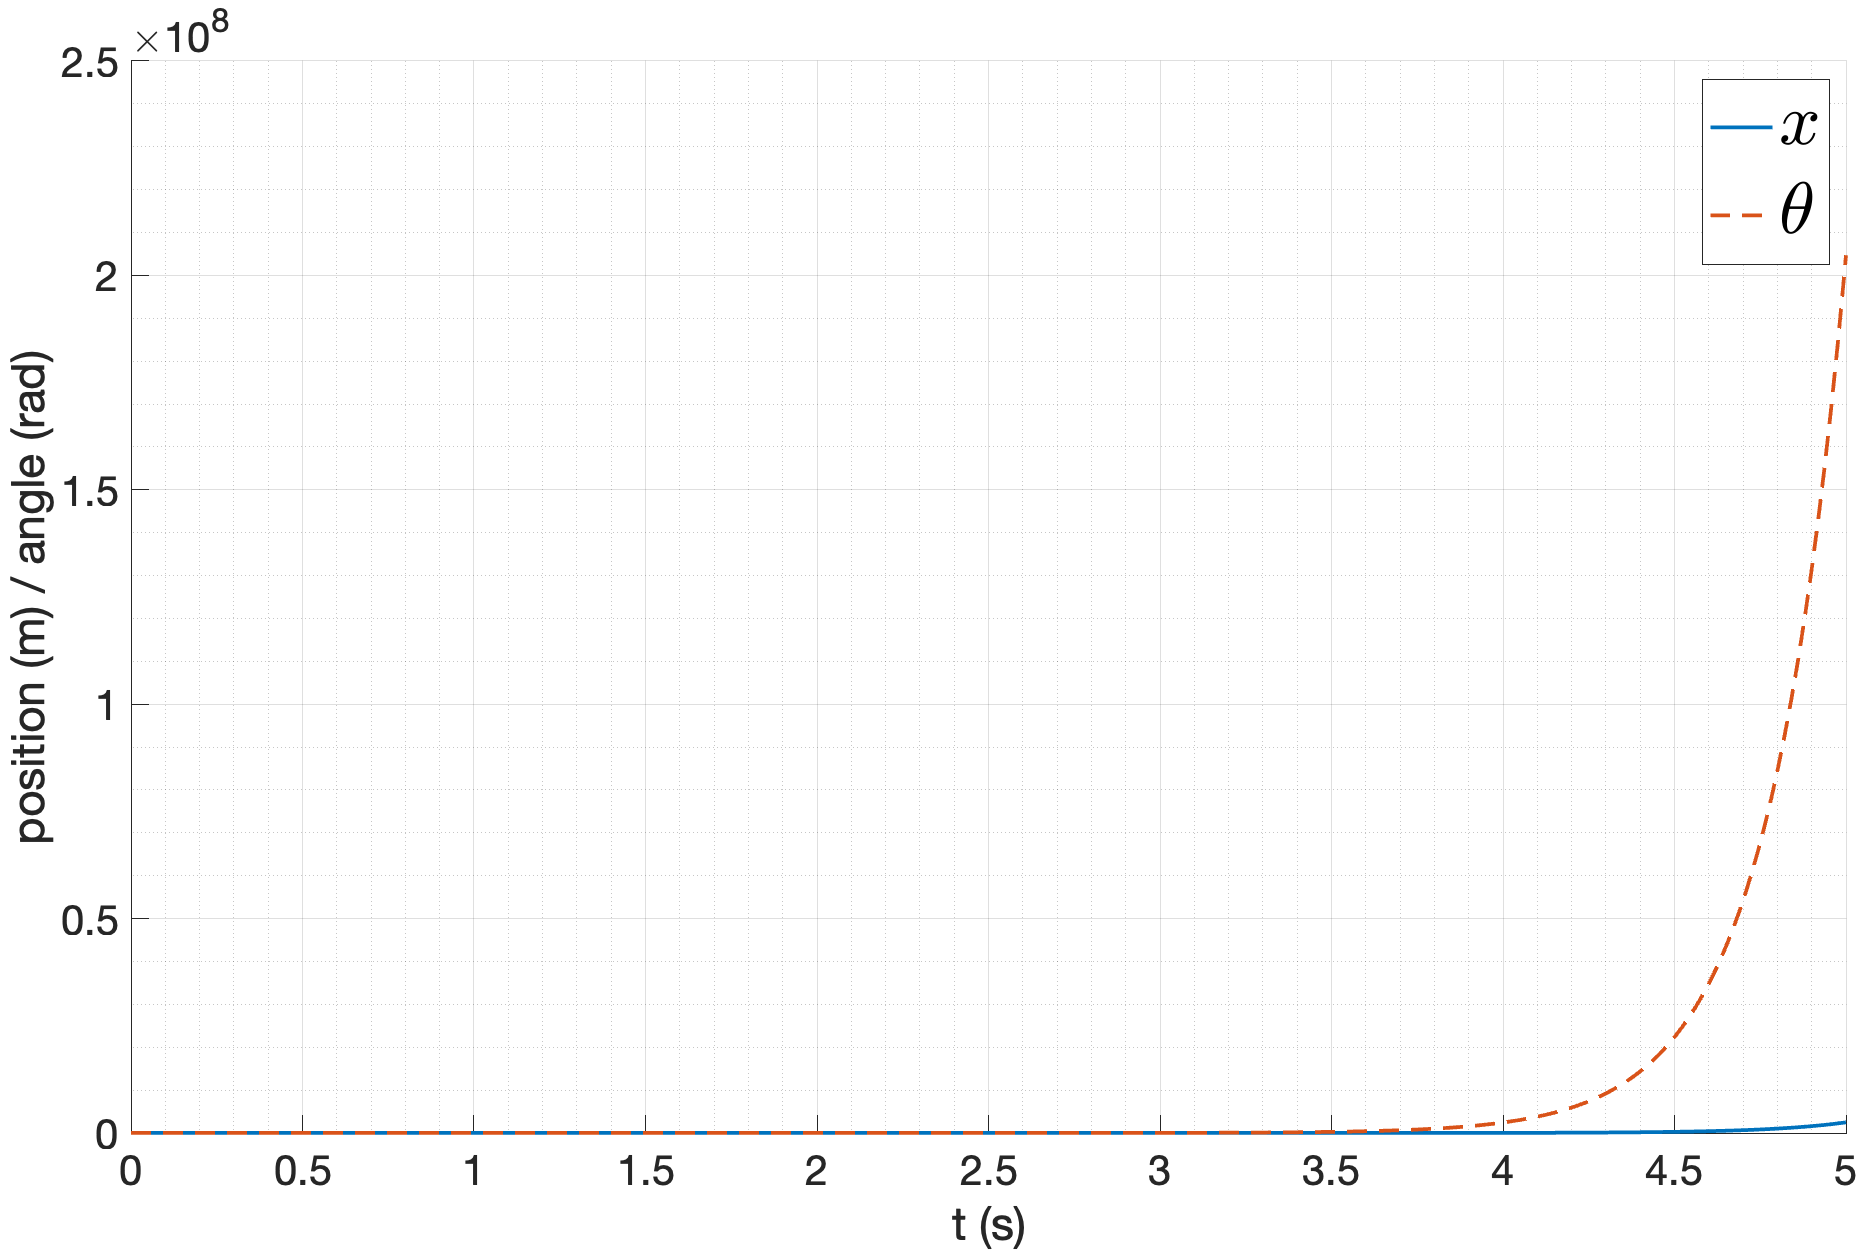
\includegraphics[width=\textwidth]{media/plots/free_motion/long_linear.png}
    \caption{Свободное движение маятника (линеаризованная модель)}
    \label{fig:free_motion_long_linear}
\end{figure}

На графиках \ref{fig:free_motion_long_nonlinear} и \ref{fig:free_motion_long_linear} видно, что
в случае нелинейной модели система колебалась с затухающими колебаниями, что является
ожидаемым результатом движения маятника, в то время как в случае линеаризованной модели система 
не является колебательной и выход системы стремится к бесконечности, это связано с тем, что
линеаризованная модель способна давать корректные результаты только в окрестности 
верхней точки равновесия, а при больших отклонениях от вертикального положения ее поведение
уже не является корректным.

\FloatBarrier
\subsubsection{Итоги моделирования}
В ходе анализа и моделирования модели системы перевернутого маятника на тележке 
и ее линеаризованной модели при небольших отклонениях от вертикального положения 
было показано, что линейная модель является хорошим приближением нелинейной модели 
в окрестности верхней точки равновесия, что позволяет использовать ее для дальнейшего
синтеза. Можно, изменив способ задания угла отклонения, получить линейную модель, 
описывающую движение маятника в окрестности нижней точки равновесия, что 
может быть использовано для создания модели козлового крана.

Из-за того, что линеаризованная модель дает корректные результаты только в окрестности 
верхней точки равновесия, асимптотическое ее поведение сильно отличается от
асимптотического поведения нелинейной модели, так же как в случае 
существенных отклонений от вертикального положения. 
\FloatBarrier
\section{Модальное управление}
\subsection{Модальный регулятор}
Рассмотрим модальный регулятор вида $u = Kx$. Согласно (\ref{eq:controlability_matrix}), система является 
полностью управляемой. Таким образом, любой спектр замкнутой системы является достижимым. 
Выберем желаемый спектр для замкнутой регулятор системы $\sigma_1 = \begin{bmatrix}-2 & -2 & -3 & -3\end{bmatrix}$. 
Для реализации регулятора, обеспечивающего заданный спектр, воспользуемся уравнением Сильвестра: 
\begin{equation}
    \begin{cases}
        AP - P\Gamma = BY \\
        K = -YP^{-1} 
    \end{cases}
\end{equation}
где $\Gamma$ -- матрица с желаемым спектром. 

Решим данное уравнение с помощью пакета \texttt{cvx} в MATLAB, в результате получаем матрицу регулятора $K$:
\begin{equation}
    K = \begin{bmatrix}
    484.11  & 806.85  & -7714.17  & -1732.95 \\ 
    \end{bmatrix}
\end{equation} 
Проверим правильность полученного результата, вычислив собственные числа замкнутой системы $A + BK$: 
\begin{equation}
    \sigma(A + BK) = \begin{bmatrix}
    -2.00 \\ 
    -2.00 \\ 
    -3.00 \\ 
    -3.00 \\ 
    \end{bmatrix}
\end{equation}
Получены желаемые собственные числа, что подтверждает правильность полученного результата. 
Рассмотрим работу регулятора на линейной модели системы при отсутствии внешних возмущений и 
небольшом начальном отклонении от равновесного состояния ($\theta_0 = 0.2$). Схема моделирования приведена на 
рисунке \ref{fig:modal_control_scheme_linear}. Результаты моделирования приведены на 
рисунке \ref{fig:modal_control_linear_out}.

\begin{figure}[ht!]
    \centering
    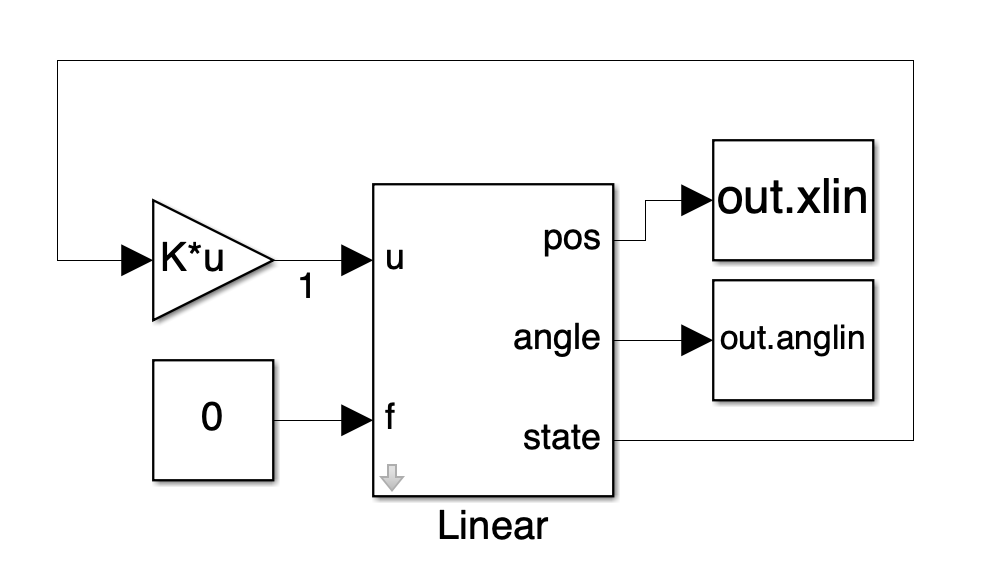
\includegraphics[width=0.7\textwidth]{media/modal_control_linear_scheme.png}
    \caption{Схема моделирования линейной модели системы с модальным регулятором}
    \label{fig:modal_control_scheme_linear}
\end{figure}
\begin{figure}[ht!]
    \centering
    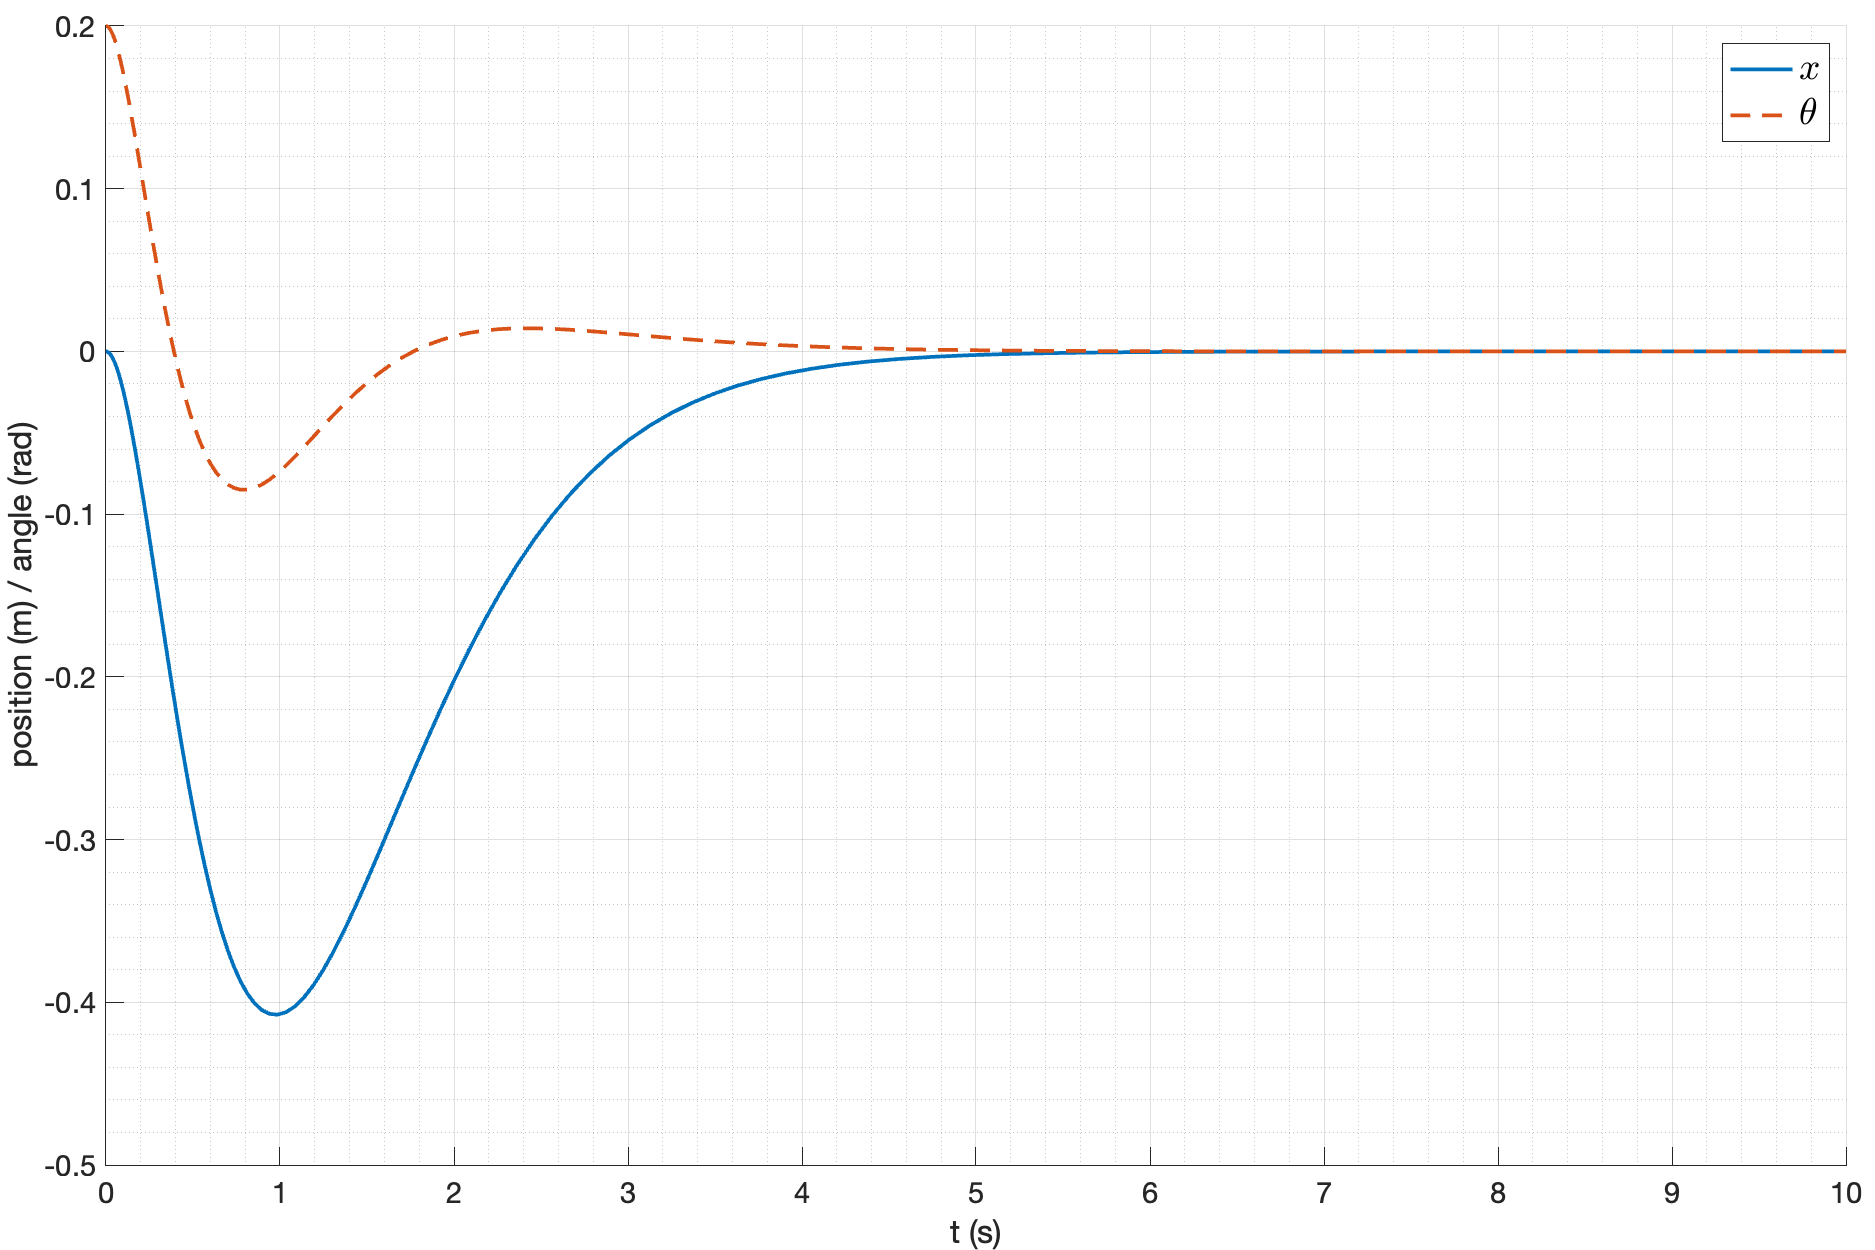
\includegraphics[width=0.8\textwidth]{media/plots/modal_control/linear_out_0.png}
    \caption{Результаты моделирования линейной модели системы с модальным регулятором}
    \label{fig:modal_control_linear_out}
\end{figure}

Можно заметить, что система приходит в равновесное состояние. Теперь попробуем использовать этот же 
модальный регулятор на нелинейной модели системы. Схема моделирования приведена на
рисунке \ref{fig:modal_control_scheme_nonlinear}. Результаты моделирования приведены на
рисунке \ref{fig:modal_control_nonlinear_out}.


\begin{figure}[ht!]
    \centering
    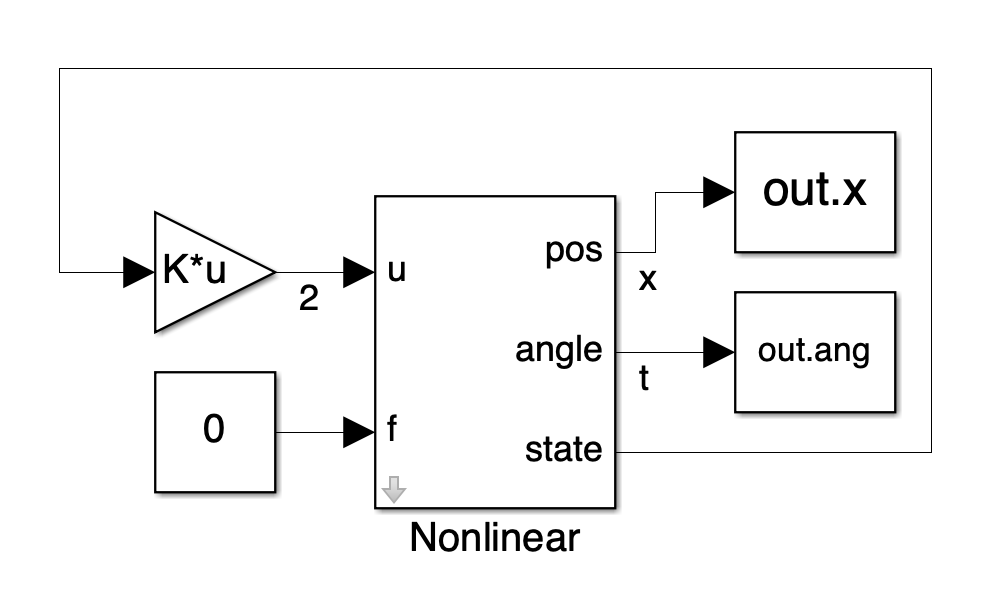
\includegraphics[width=0.7\textwidth]{media/modal_control_scheme.png}
    \caption{Схема моделирования нелинейной модели системы с модальным регулятором}
    \label{fig:modal_control_scheme_nonlinear}
\end{figure}
\begin{figure}[ht!]
    \centering
    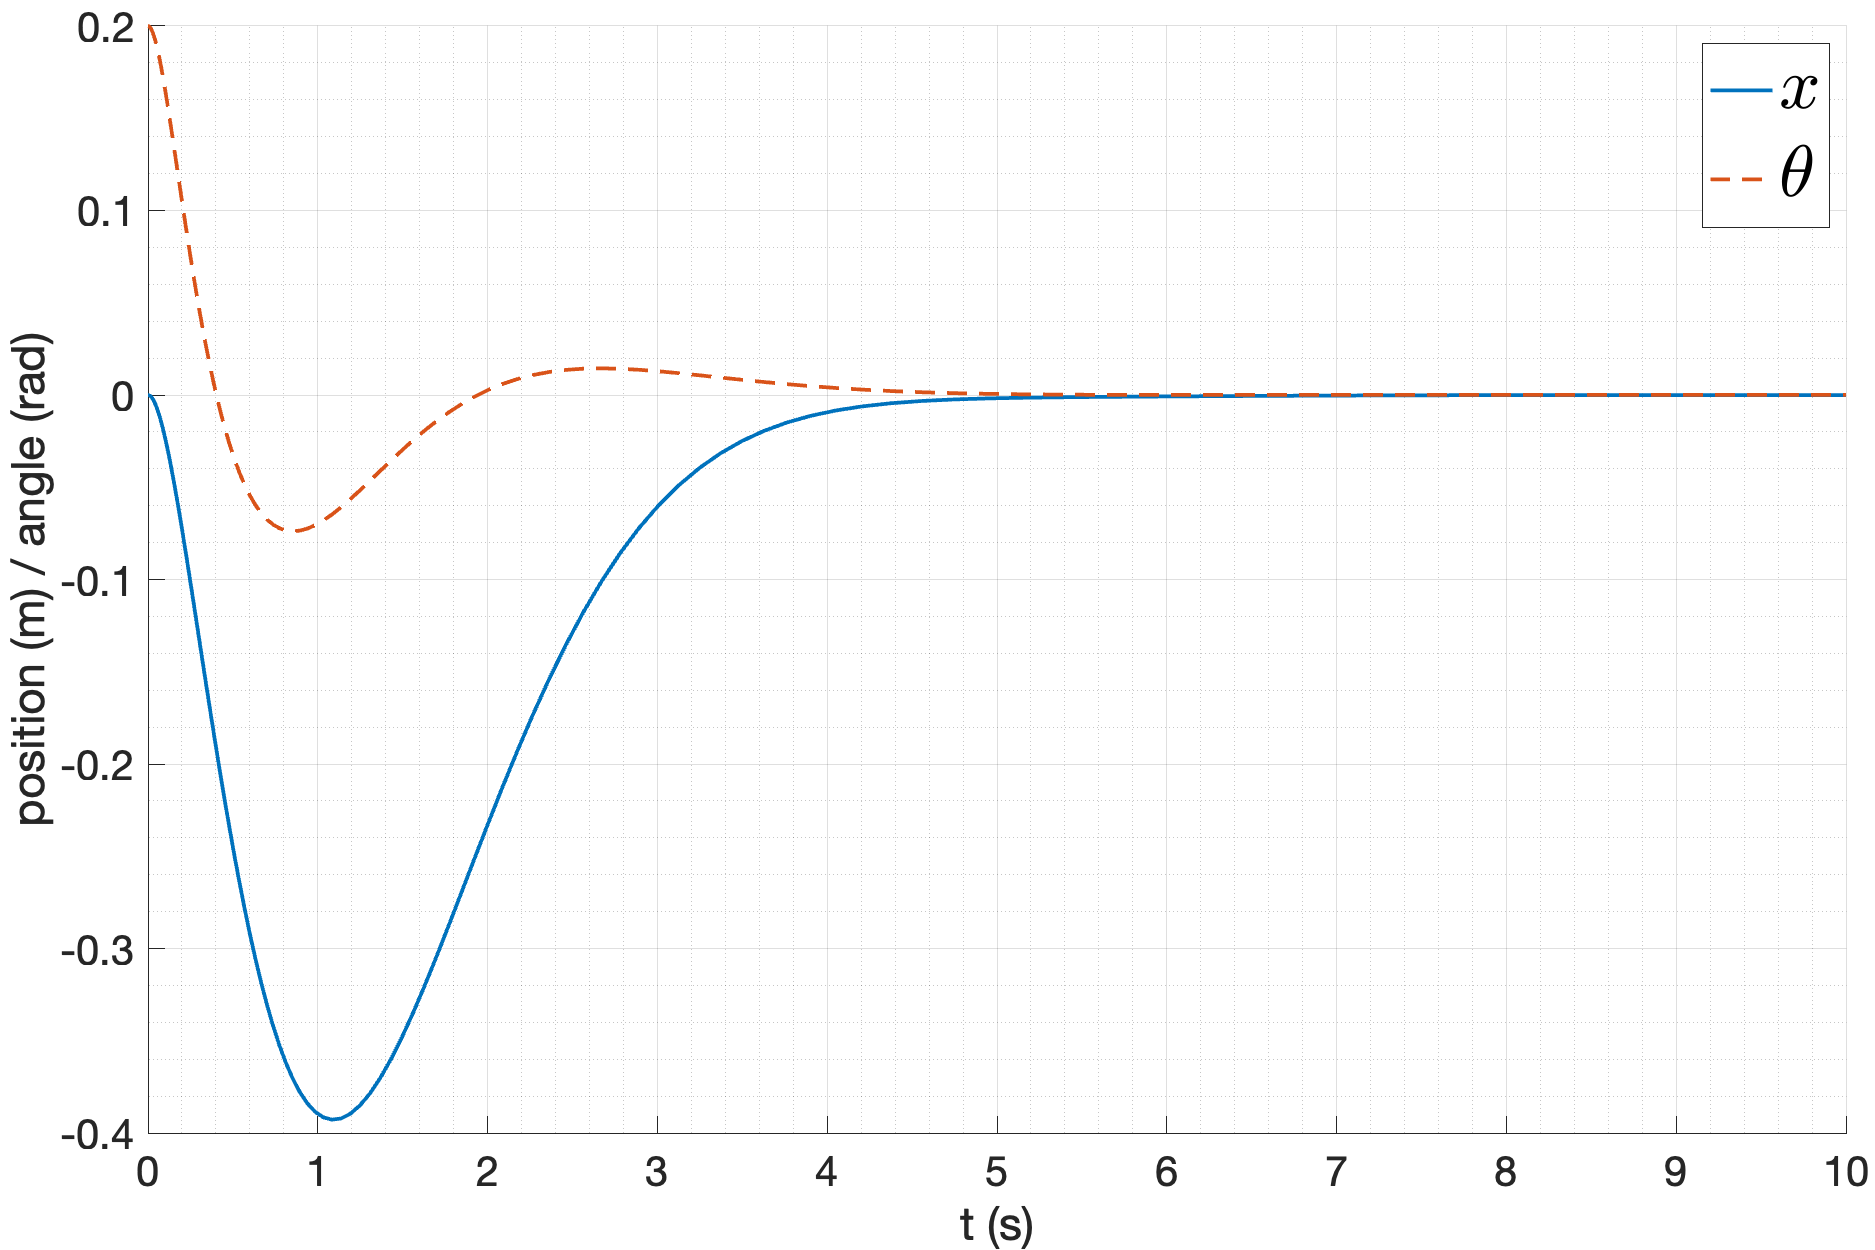
\includegraphics[width=0.8\textwidth]{media/plots/modal_control/out_0.png}
    \caption{Результаты моделирования нелинейной модели системы с модальным регулятором}
    \label{fig:modal_control_nonlinear_out}
\end{figure}

Рассмотрим различия между движением линейной и нелинейной модели системы. График различий в движении
представлен на рисунке \ref{fig:modal_control_cmp}.
\begin{figure}[ht!]
    \centering
    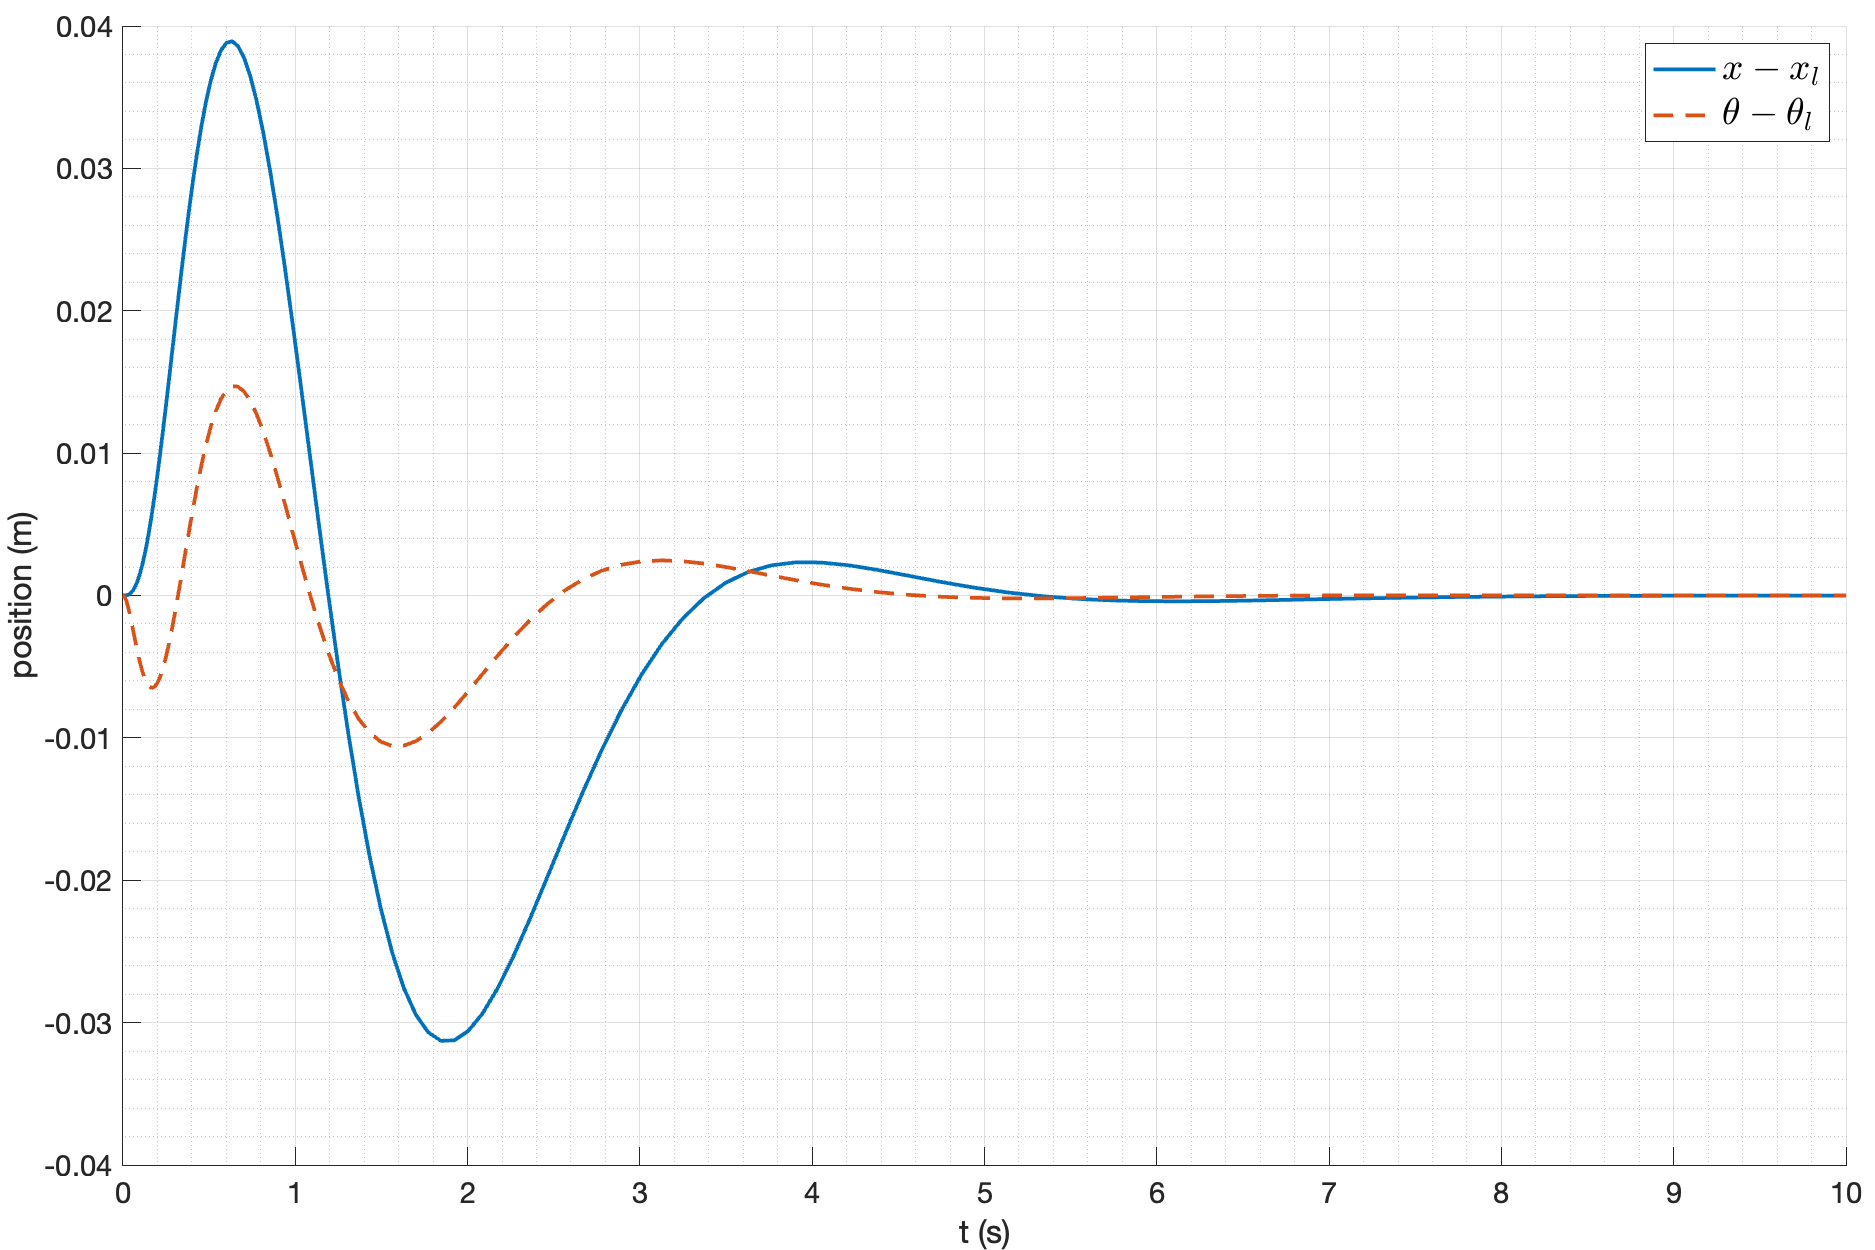
\includegraphics[width=0.8\textwidth]{media/plots/modal_control/cmp_0.png}
    \caption{Различия в движении линейной и нелинейной модели системы с модальным регулятором}
    \label{fig:modal_control_cmp}
\end{figure}
Видно, что различие между углом отклонения маятника не превышает $2 \cdot 10^{-2}$ радиан, а различие между
координатами тележки не превышает $4\cdot10^{-2}$ метра. Данный результат можно считать удовлетворительным, 
регулятор, синтезированный для линейной модели системы, обеспечивает приемлемое качество управления 
нелинейной модели системы. 

\FloatBarrier
\subsection{Исследование устойчивости при различных начальных условиях}
Проверим работу данного регулятора при различных начальных условиях. 
В качестве начальных условий возьмем различные начальные углы отклонения маятника $\theta_0 \in \begin{bmatrix}0.3, 0.7, 0.9, 1.0, 1.1, 1.2\end{bmatrix}$. Результаты 
моделирования приведены на рисунке \ref{fig:modal_control_initials}. 
\begin{figure}[ht!]
    \centering
    \begin{subfigure}[b]{0.45\textwidth}
        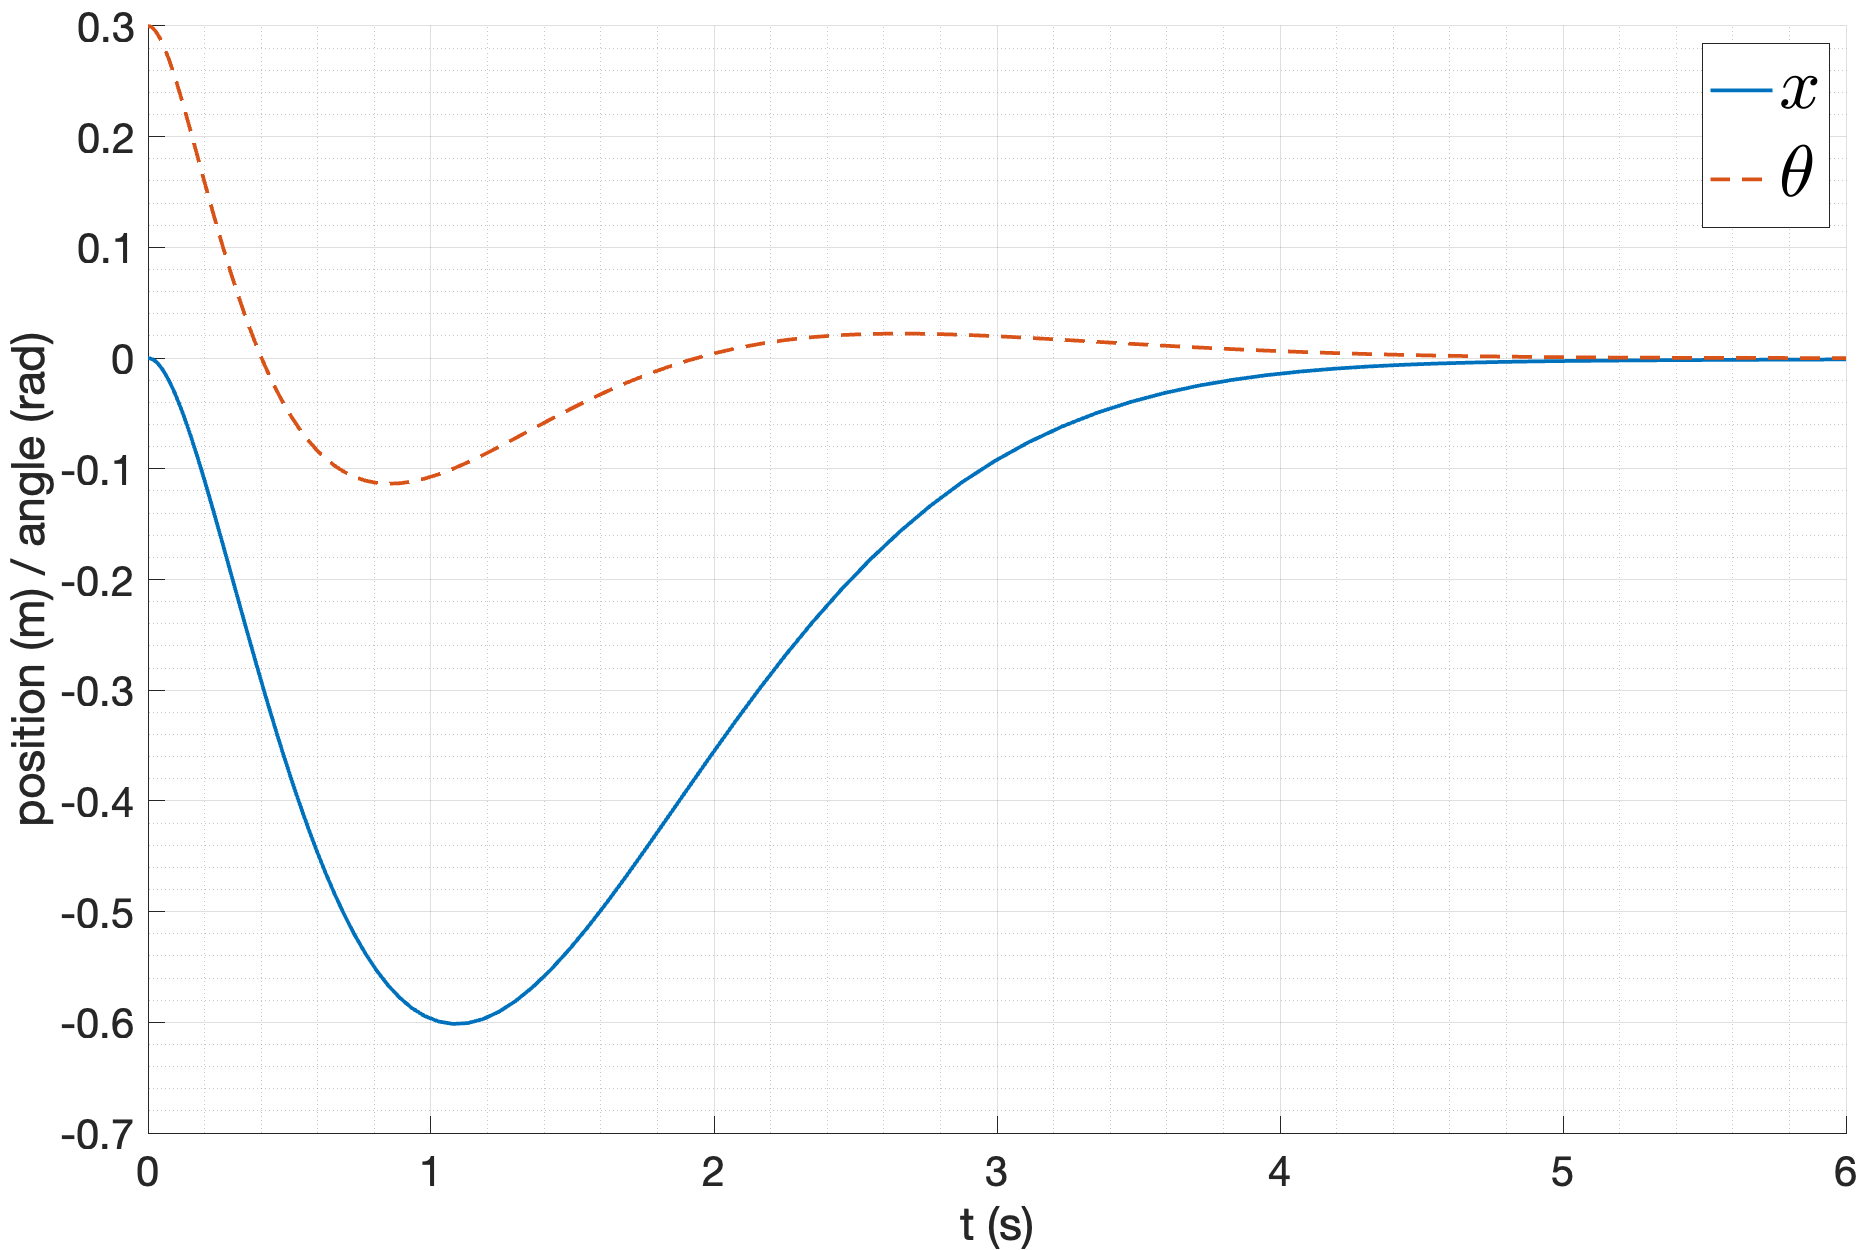
\includegraphics[width=\textwidth]{media/plots/modal_control/out_1.png}
        \caption{$\theta_0 = 0.3$}
    \end{subfigure}
    \begin{subfigure}[b]{0.45\textwidth}
        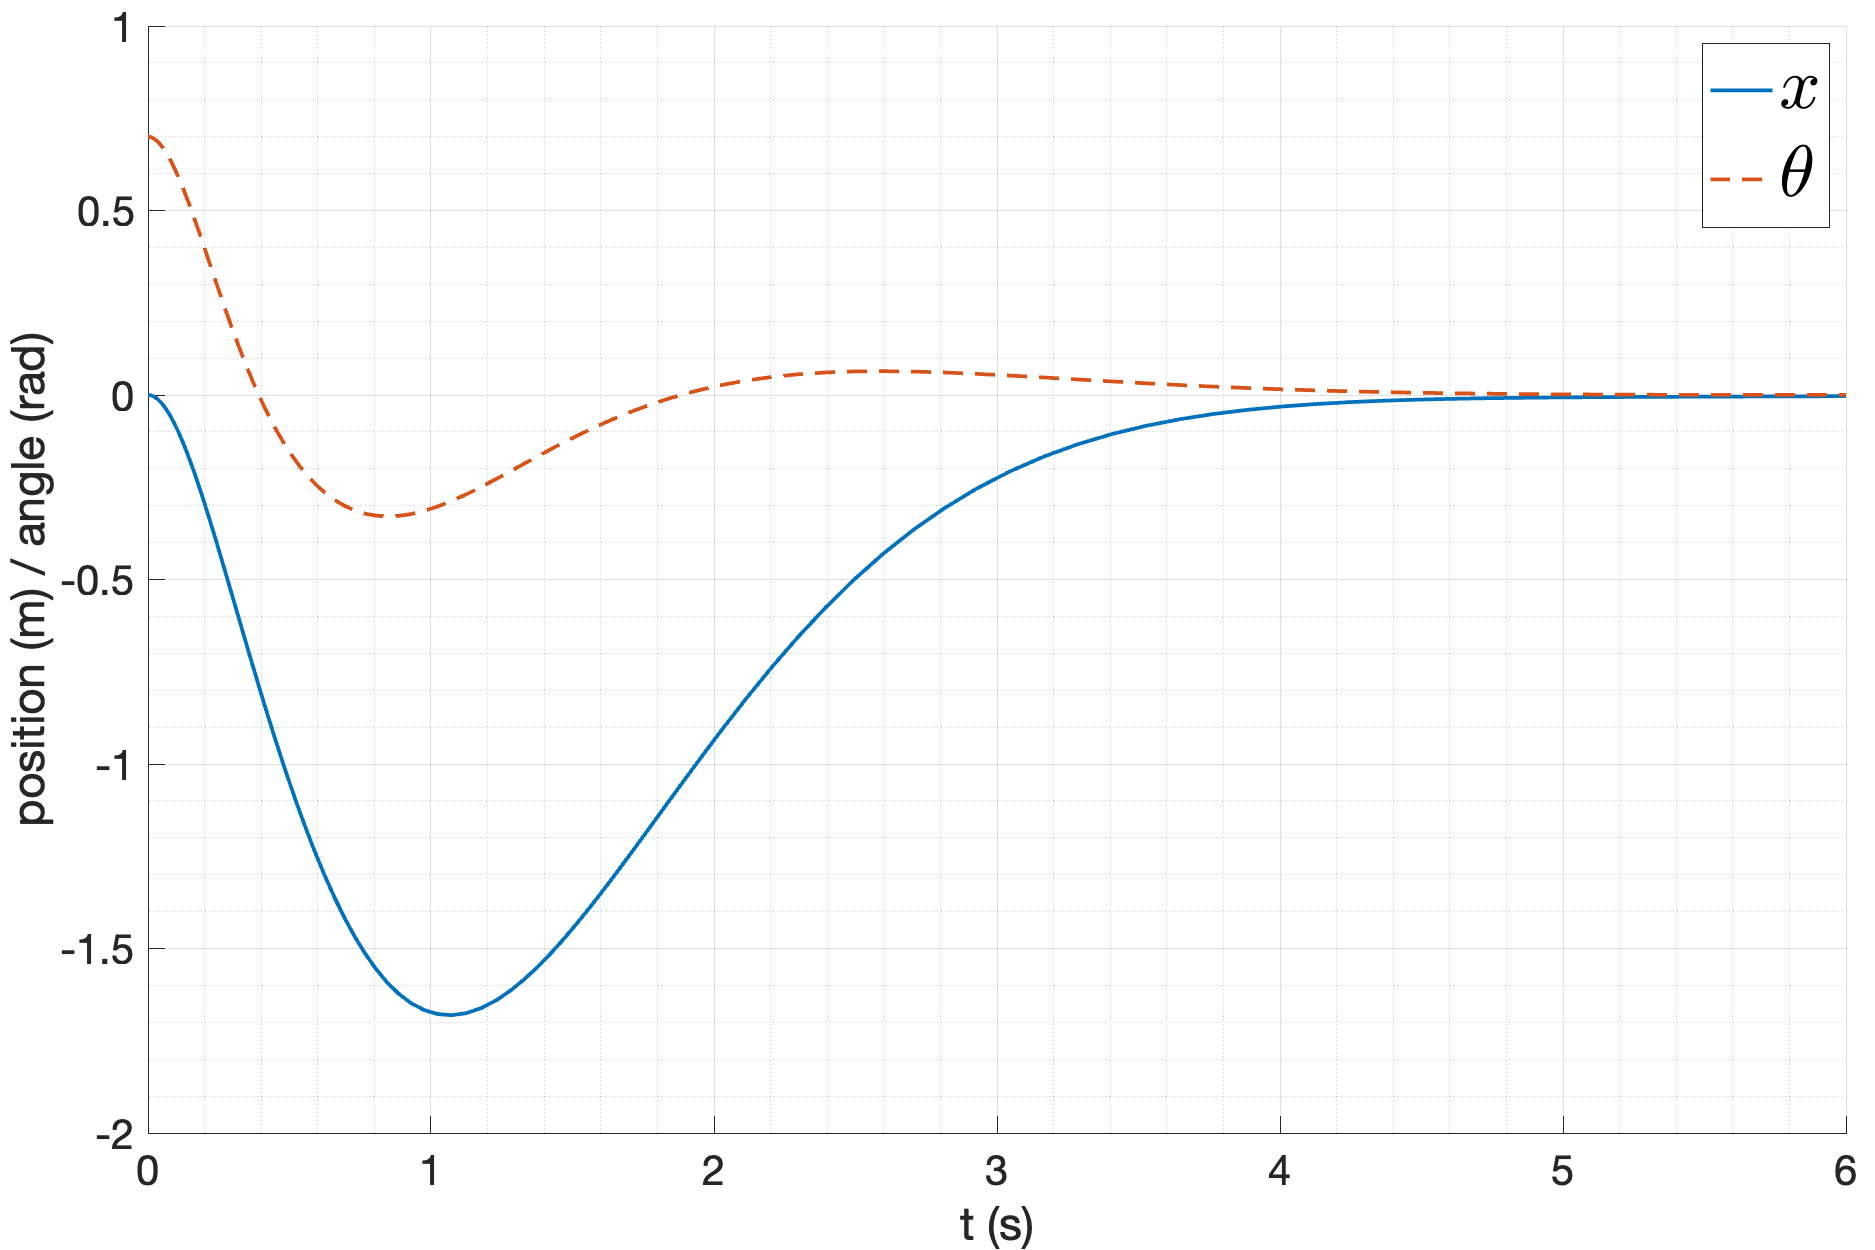
\includegraphics[width=\textwidth]{media/plots/modal_control/out_2.png}
        \caption{$\theta_0 = 0.7$}
    \end{subfigure}
    \begin{subfigure}[b]{0.45\textwidth}
        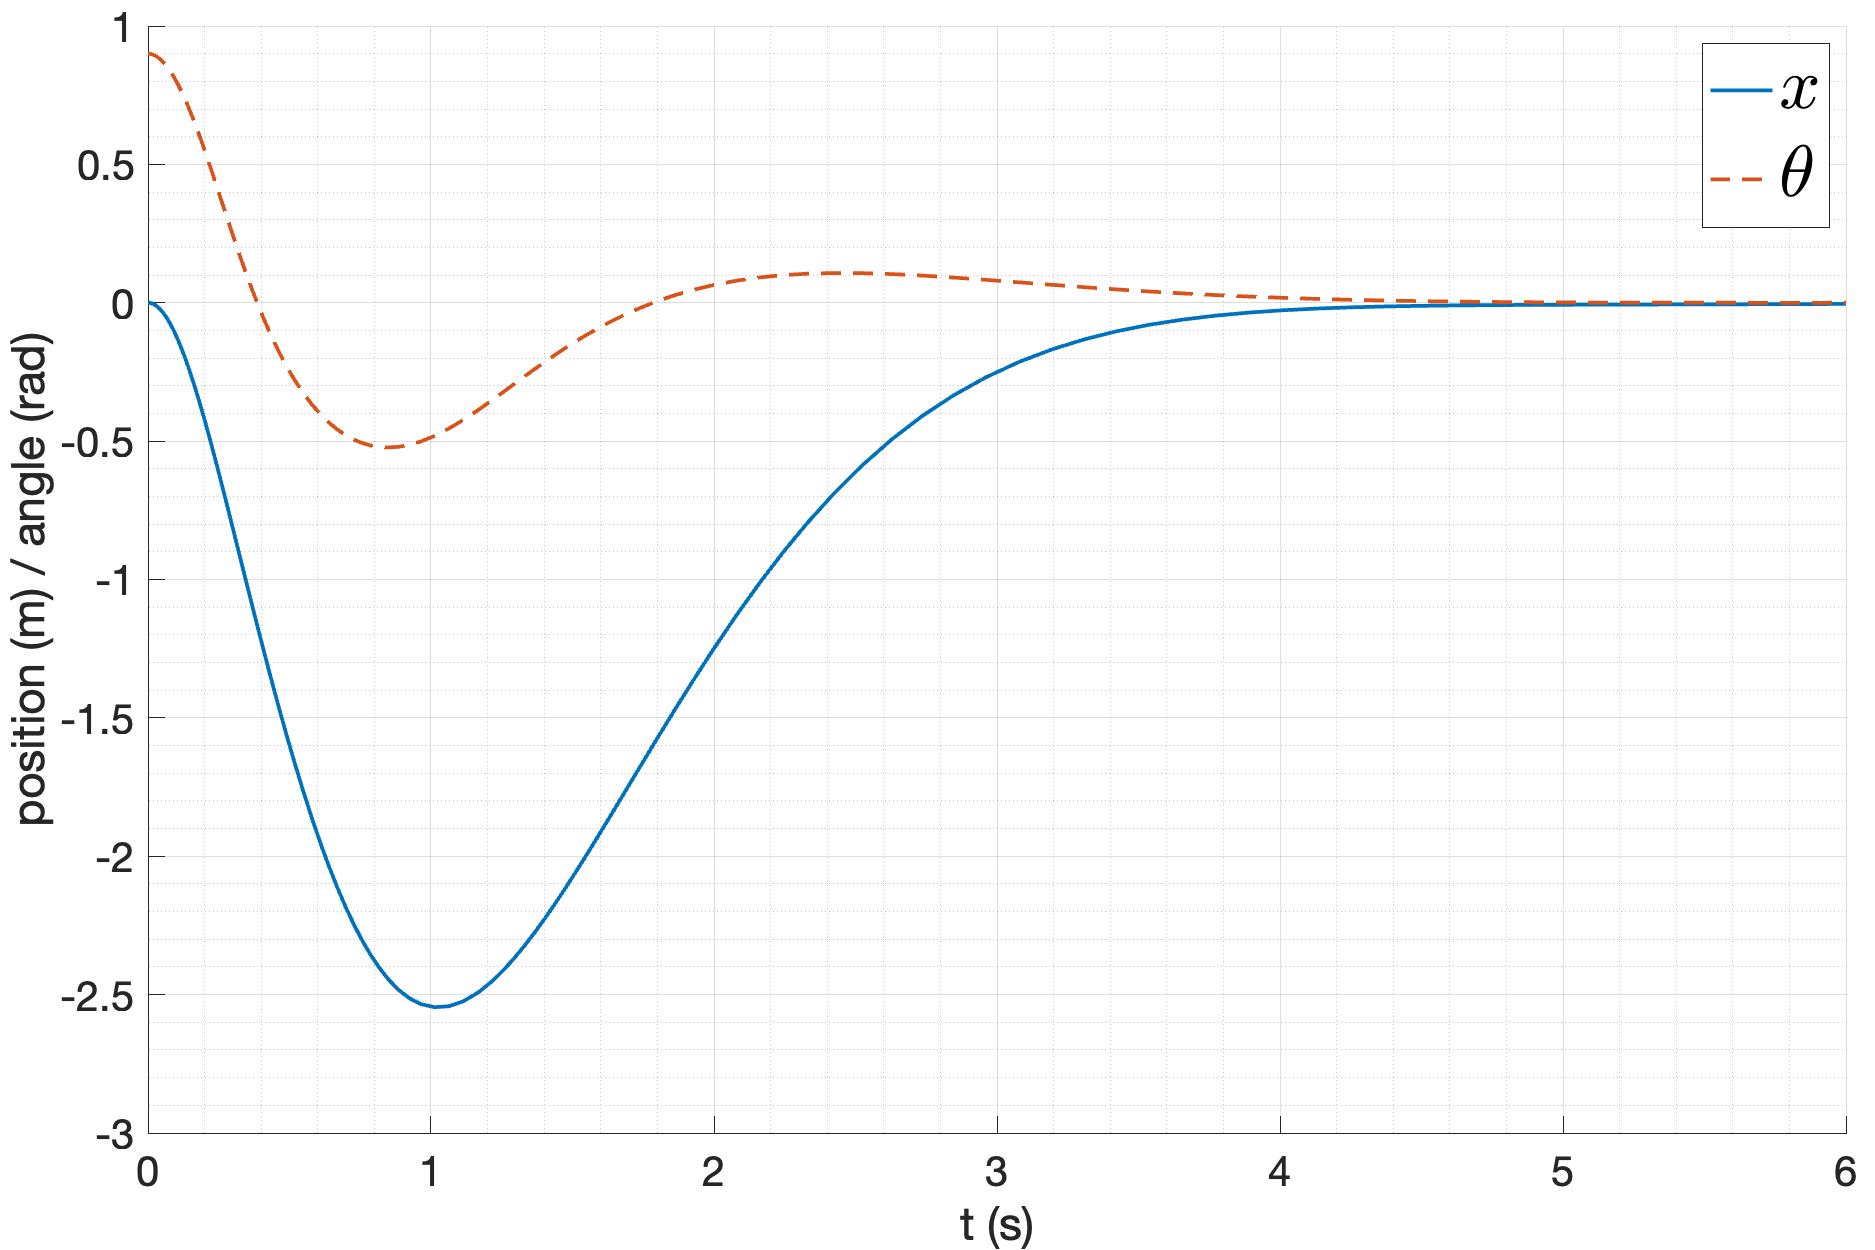
\includegraphics[width=\textwidth]{media/plots/modal_control/out_3.png}
        \caption{$\theta_0 = 0.9$}
    \end{subfigure}
    \begin{subfigure}[b]{0.45\textwidth}
        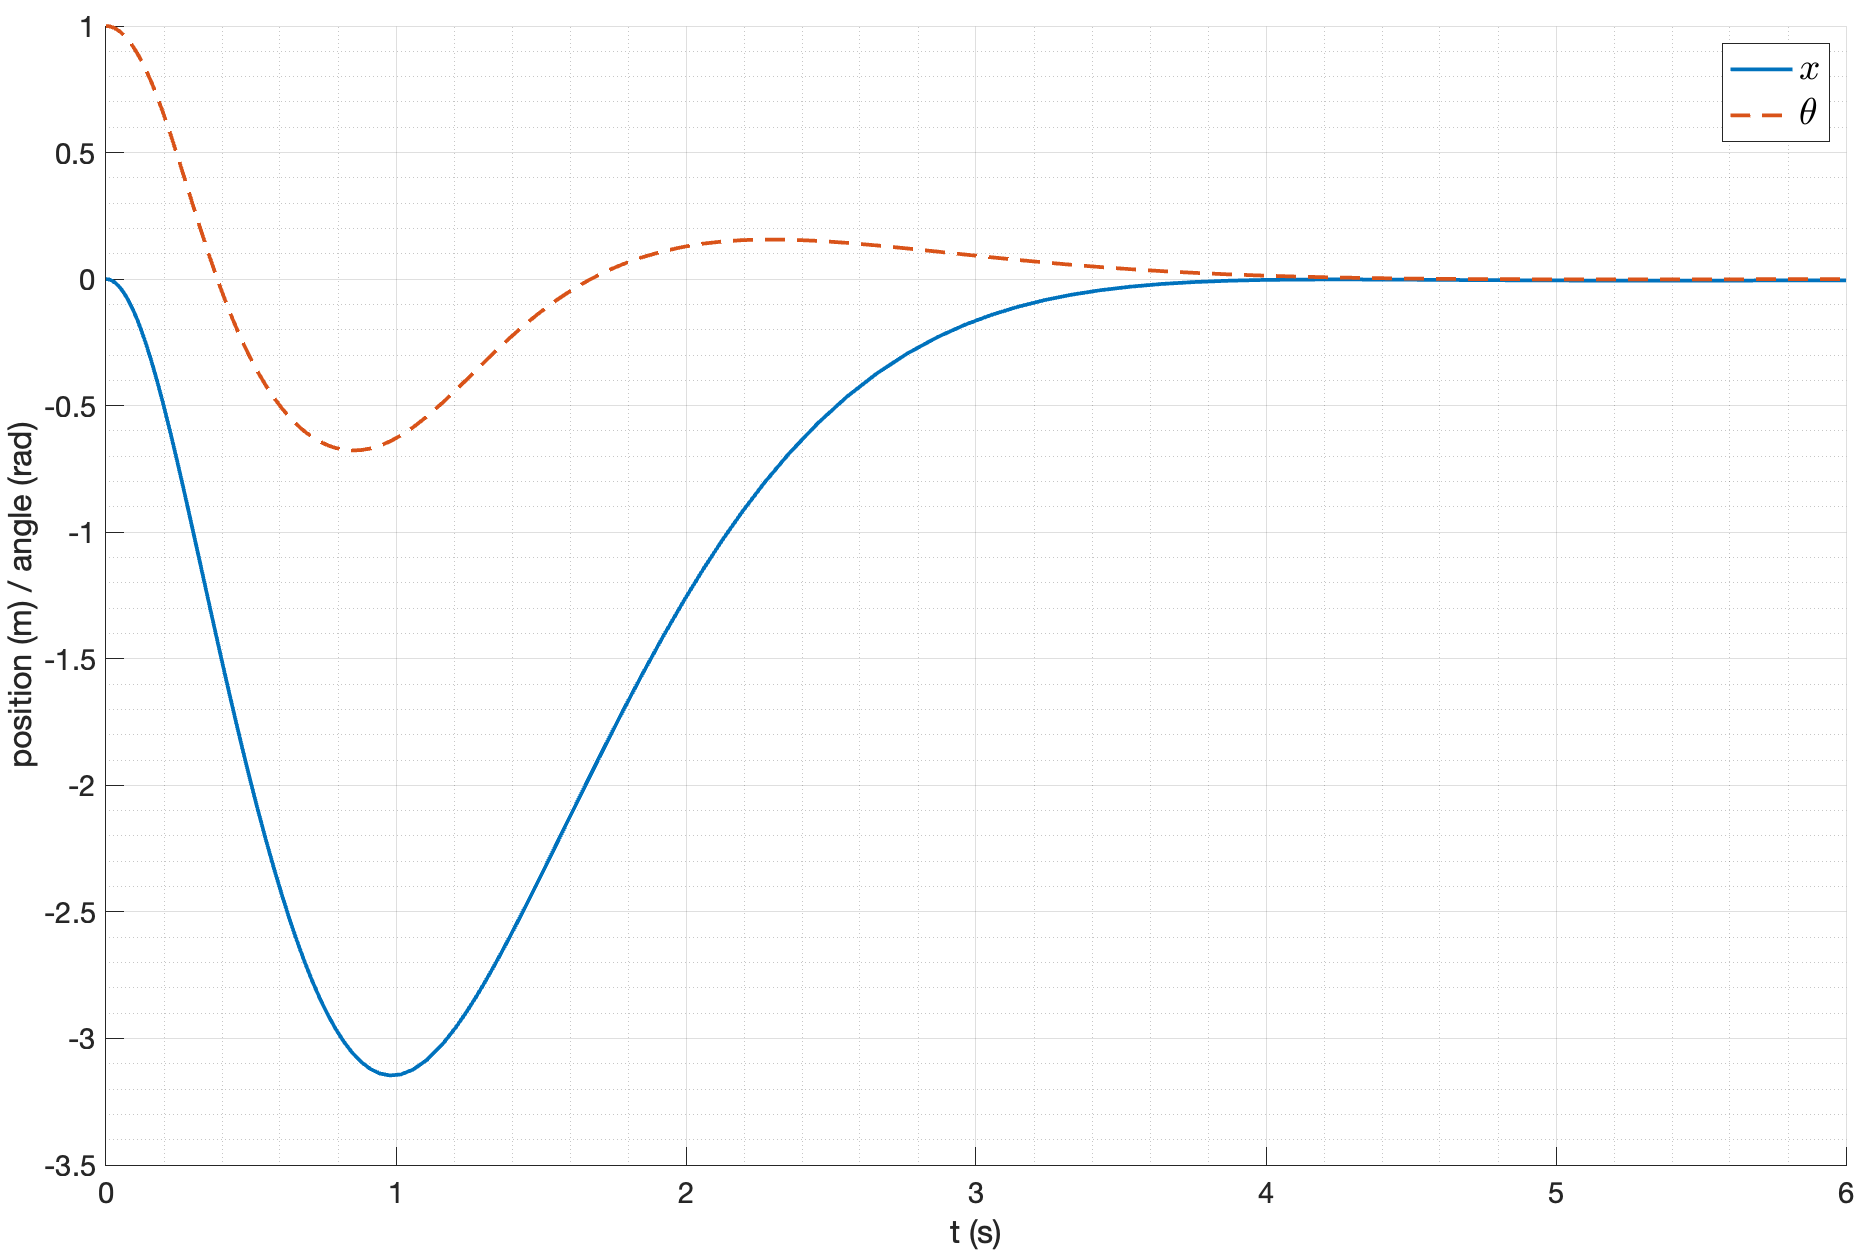
\includegraphics[width=\textwidth]{media/plots/modal_control/out_4.png}
        \caption{$\theta_0 = 1.0$}
    \end{subfigure}
    \begin{subfigure}[b]{0.45\textwidth}
        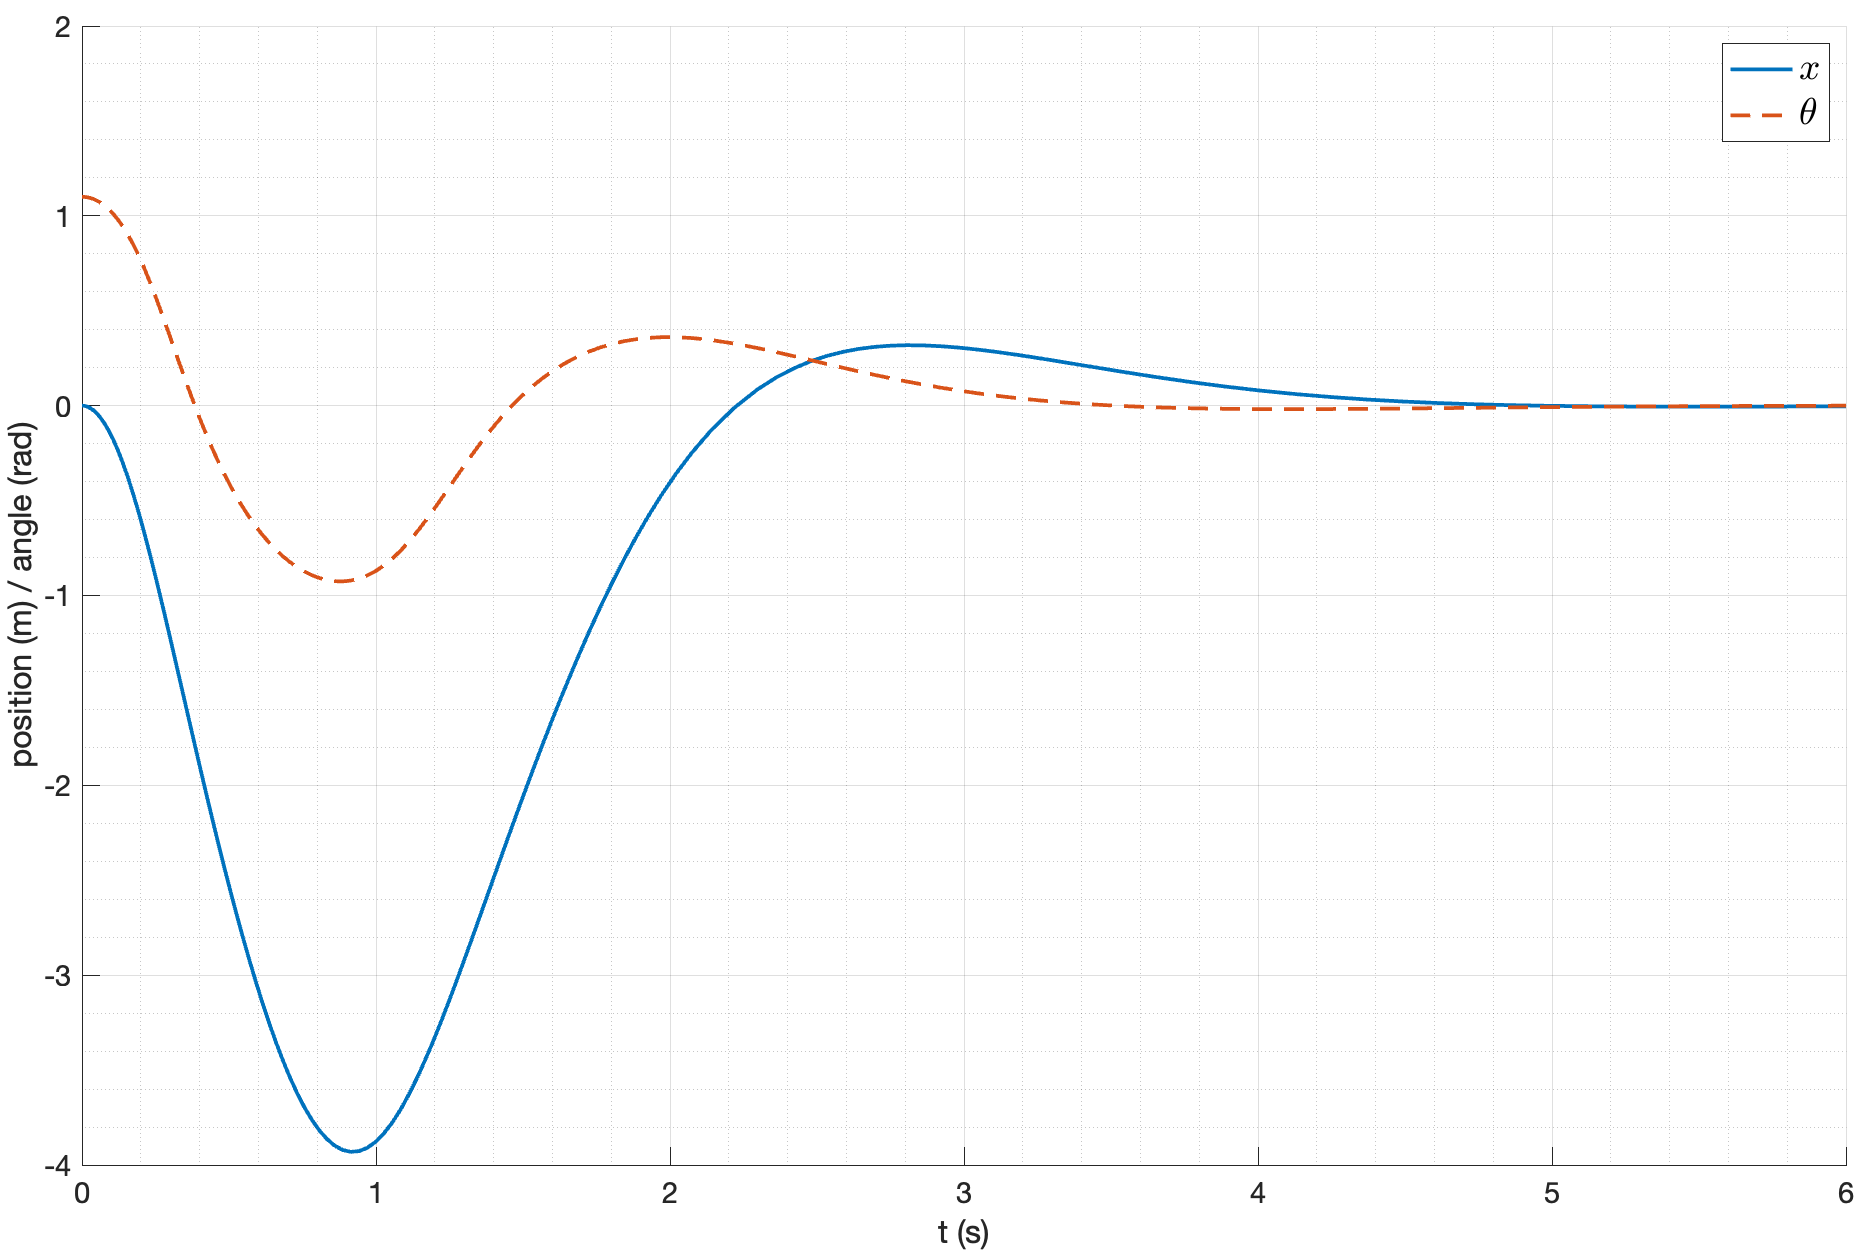
\includegraphics[width=\textwidth]{media/plots/modal_control/out_5.png}
        \caption{$\theta_0 = 1.1$}
    \end{subfigure}
    \begin{subfigure}[b]{0.45\textwidth}
        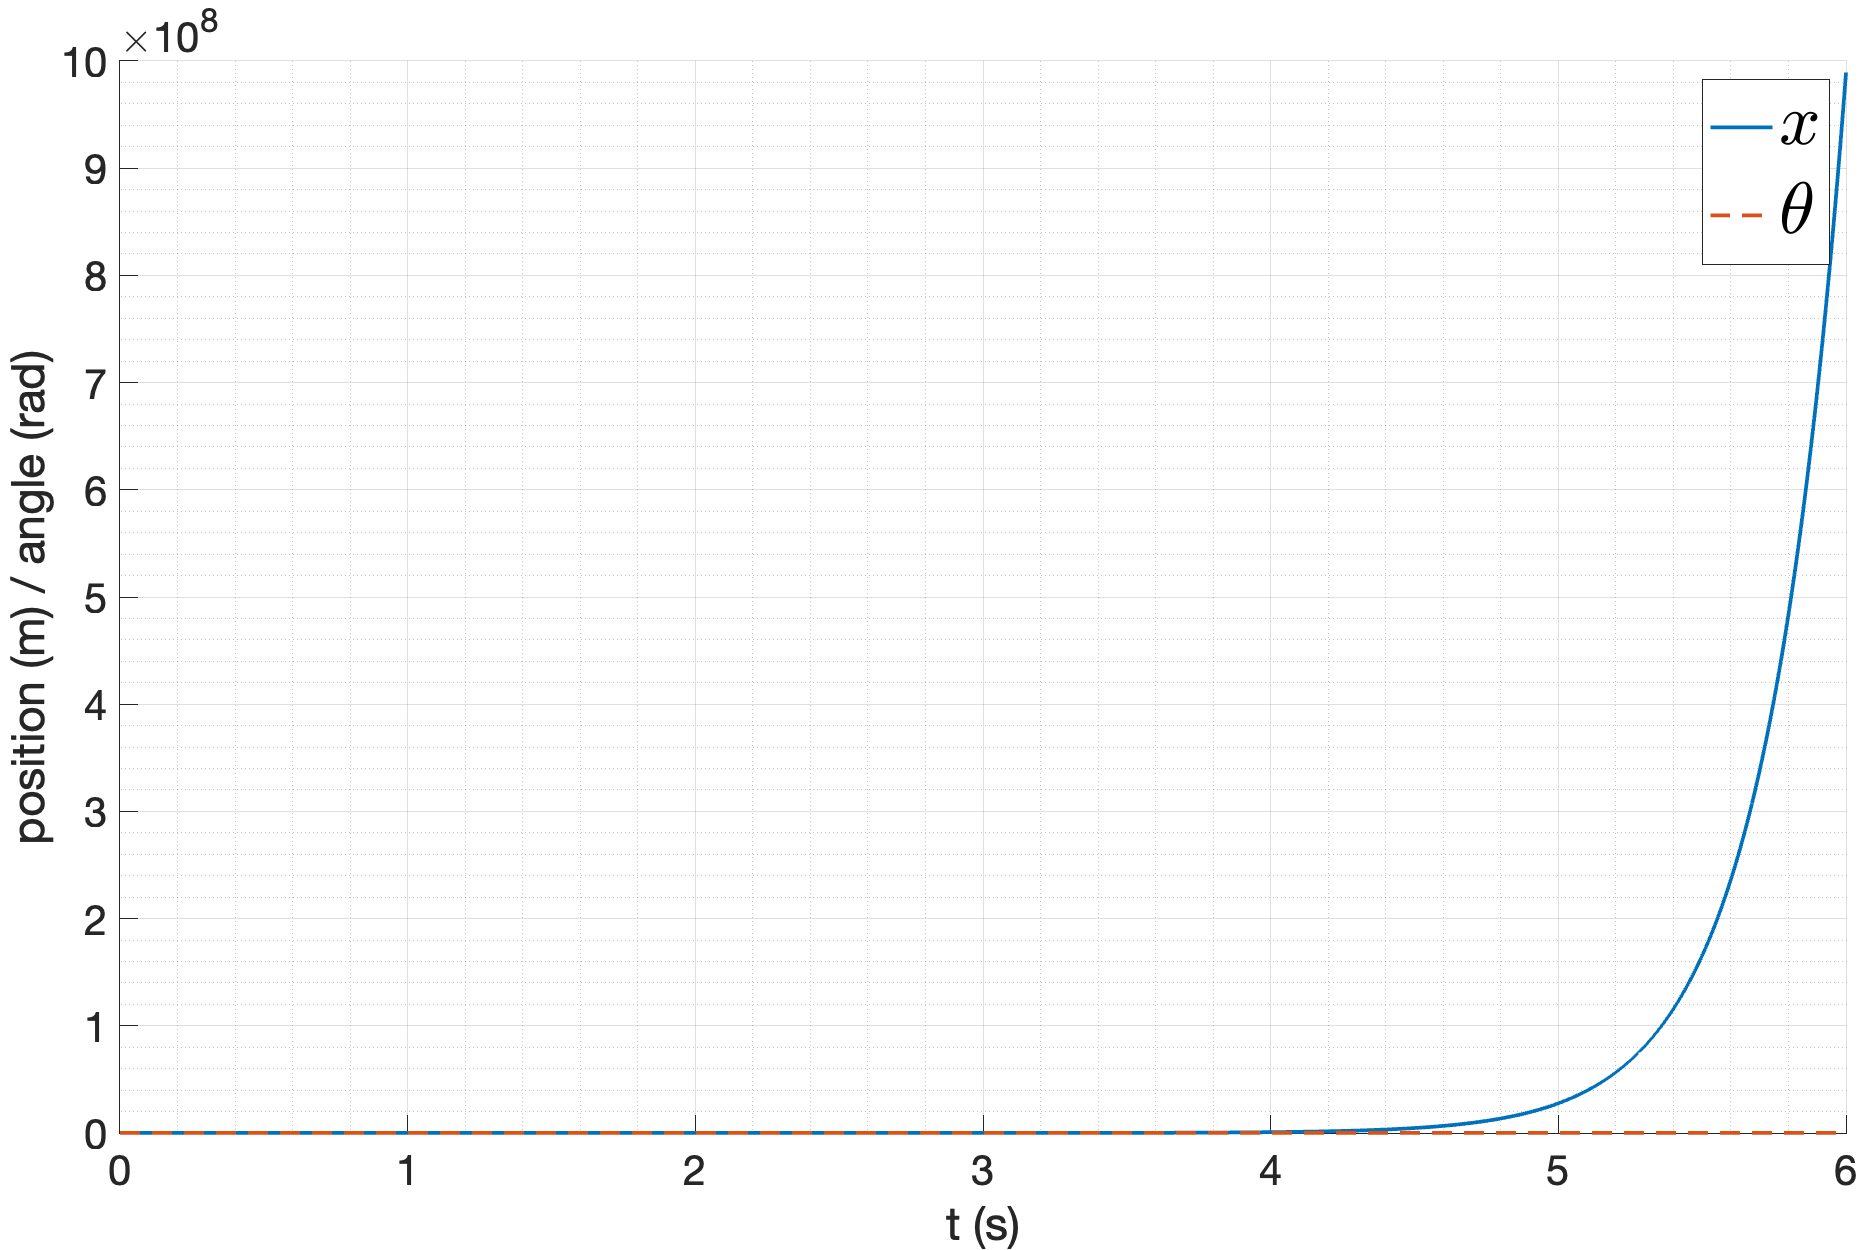
\includegraphics[width=\textwidth]{media/plots/modal_control/out_6.png}
        \caption{$\theta_0 = 1.2$}
    \end{subfigure}
    \caption{Модальное управление нелинейной модели системы}
    \label{fig:modal_control_initials}
\end{figure}
Видно, что при начальном угле отклонения маятника вплоть до $\theta_0 = 1.0$ система приходит в
равновесное состояние. При этом время переходного процесса остается приблизительно одинаковым. 
При дальнейшем увеличении угла начального отклонения маятника система не приходит в равновесное состояние, 
это связано с тем, что при больших отклонениях маятника от вертикального положения линейная модель, на основе 
которой был синтезирован регулятор, перестает адекватно описывать поведение системы. Убедиться в этом можно 
посмотрев на график поведения линейной модели системы при начальном угле отклонения $\theta_0 = 1.2$ (рисунок \ref{fig:modal_control_linear_out_6}).
\begin{figure}[ht!]
    \centering
    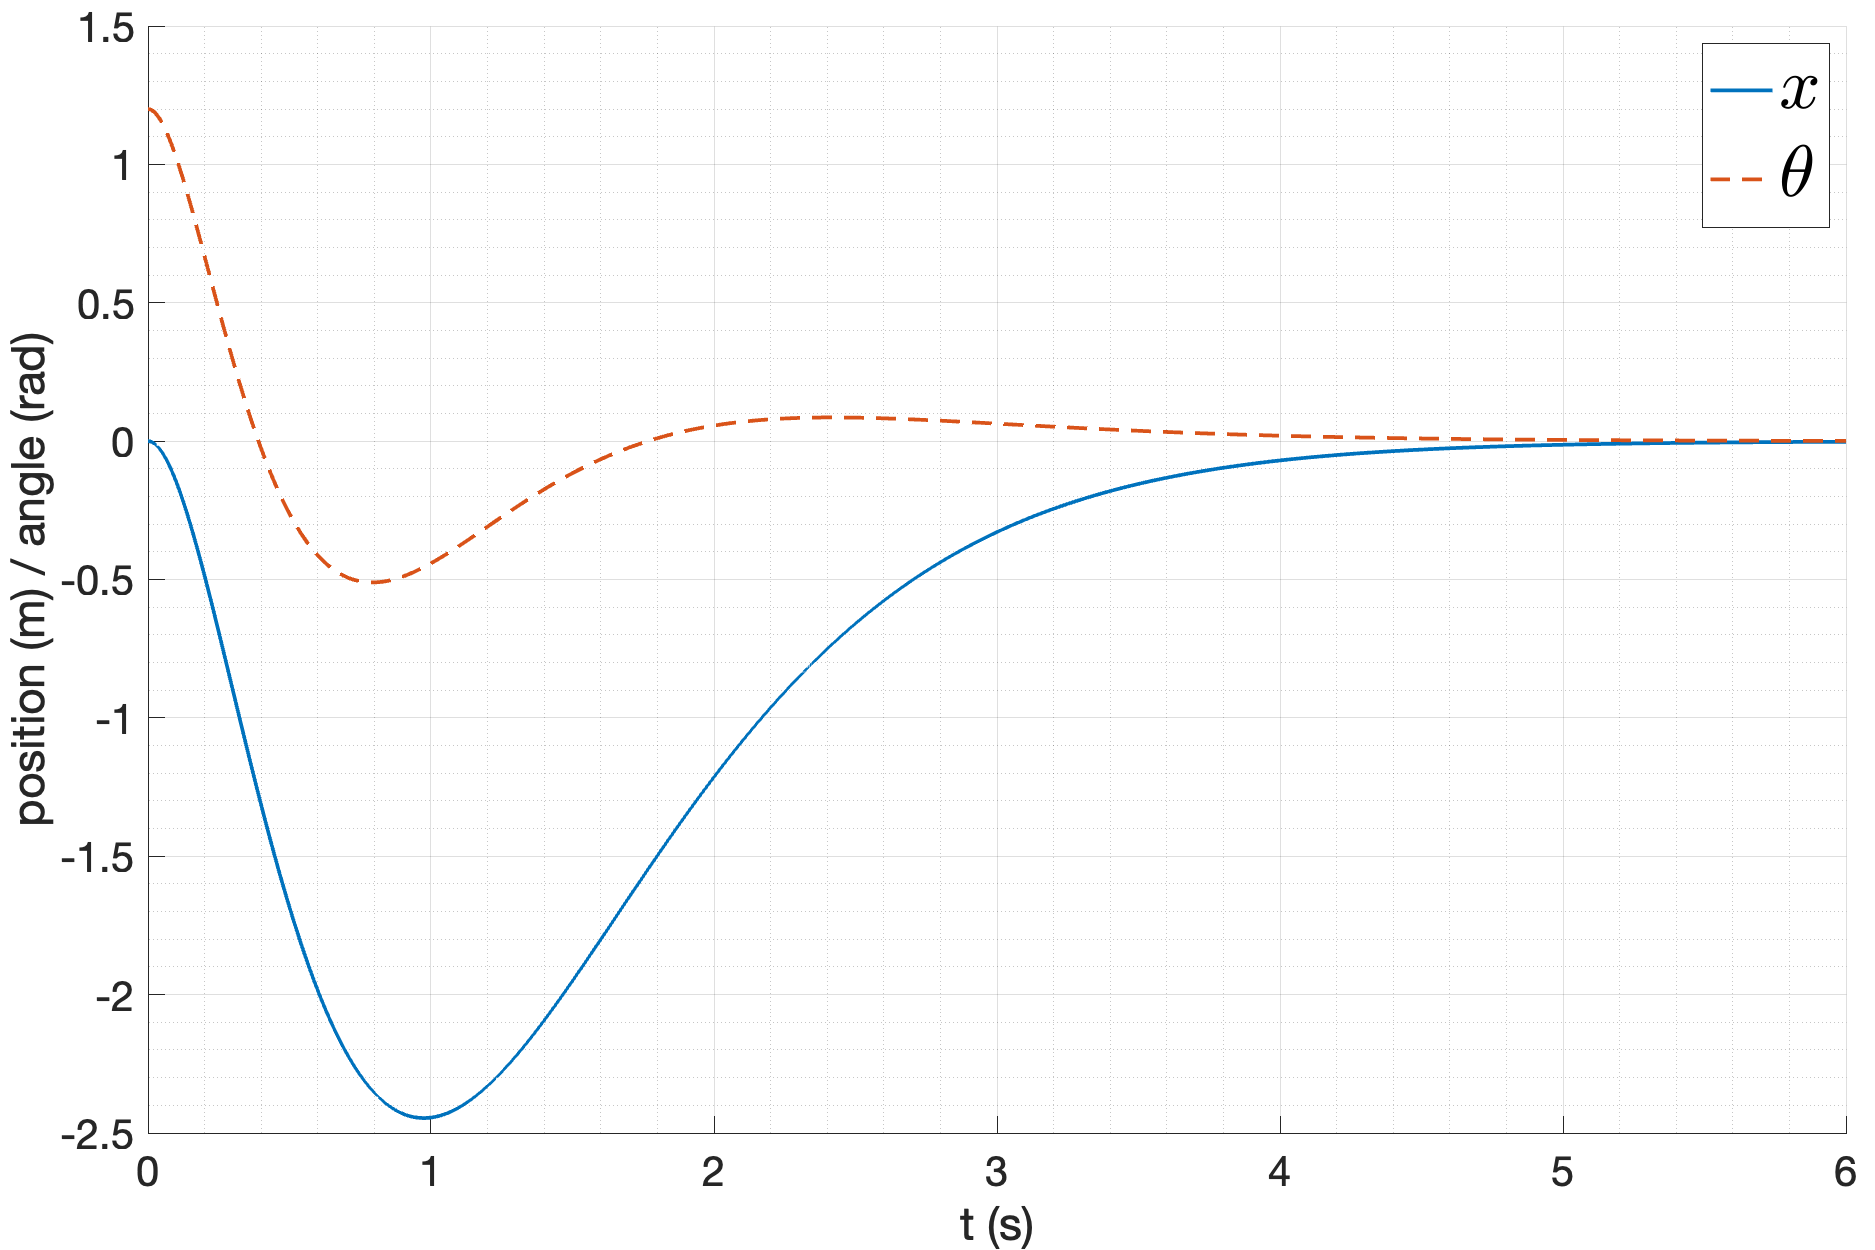
\includegraphics[width=\textwidth]{media/plots/modal_control/linear_out_6.png}
    \caption{Результаты моделирования линейной модели системы с модальным регулятором при $\theta_0 = 1.2$}
    \label{fig:modal_control_linear_out_6}
\end{figure}
\FloatBarrier
Видно, что линейная модель система приходит в равновесное состояния, в отличие от нелинейной модели.

\subsection{Исследование переходного процесса}
Будем рассматривать переходный процесс и управляющее воздействие при различных собственных числах замкнутой регулятором системы. 
В качестве начальных условий возьмем $\theta_0 = 0.3$. Для начала, рассмотрим регуляторы, обеспечивающие спектр 
замкнутой системы вида $\sigma_k = \begin{bmatrix}k & k & k & k\end{bmatrix}$, где $k \in \begin{bmatrix}-4, -6, -8, -10\end{bmatrix}$. 
Результаты моделирования приведены на рисунках \ref{fig:modal_controlers_1_out} -- \ref{fig:modal_controlers_4_u}.

\begin{figure}[ht!]
    \centering
    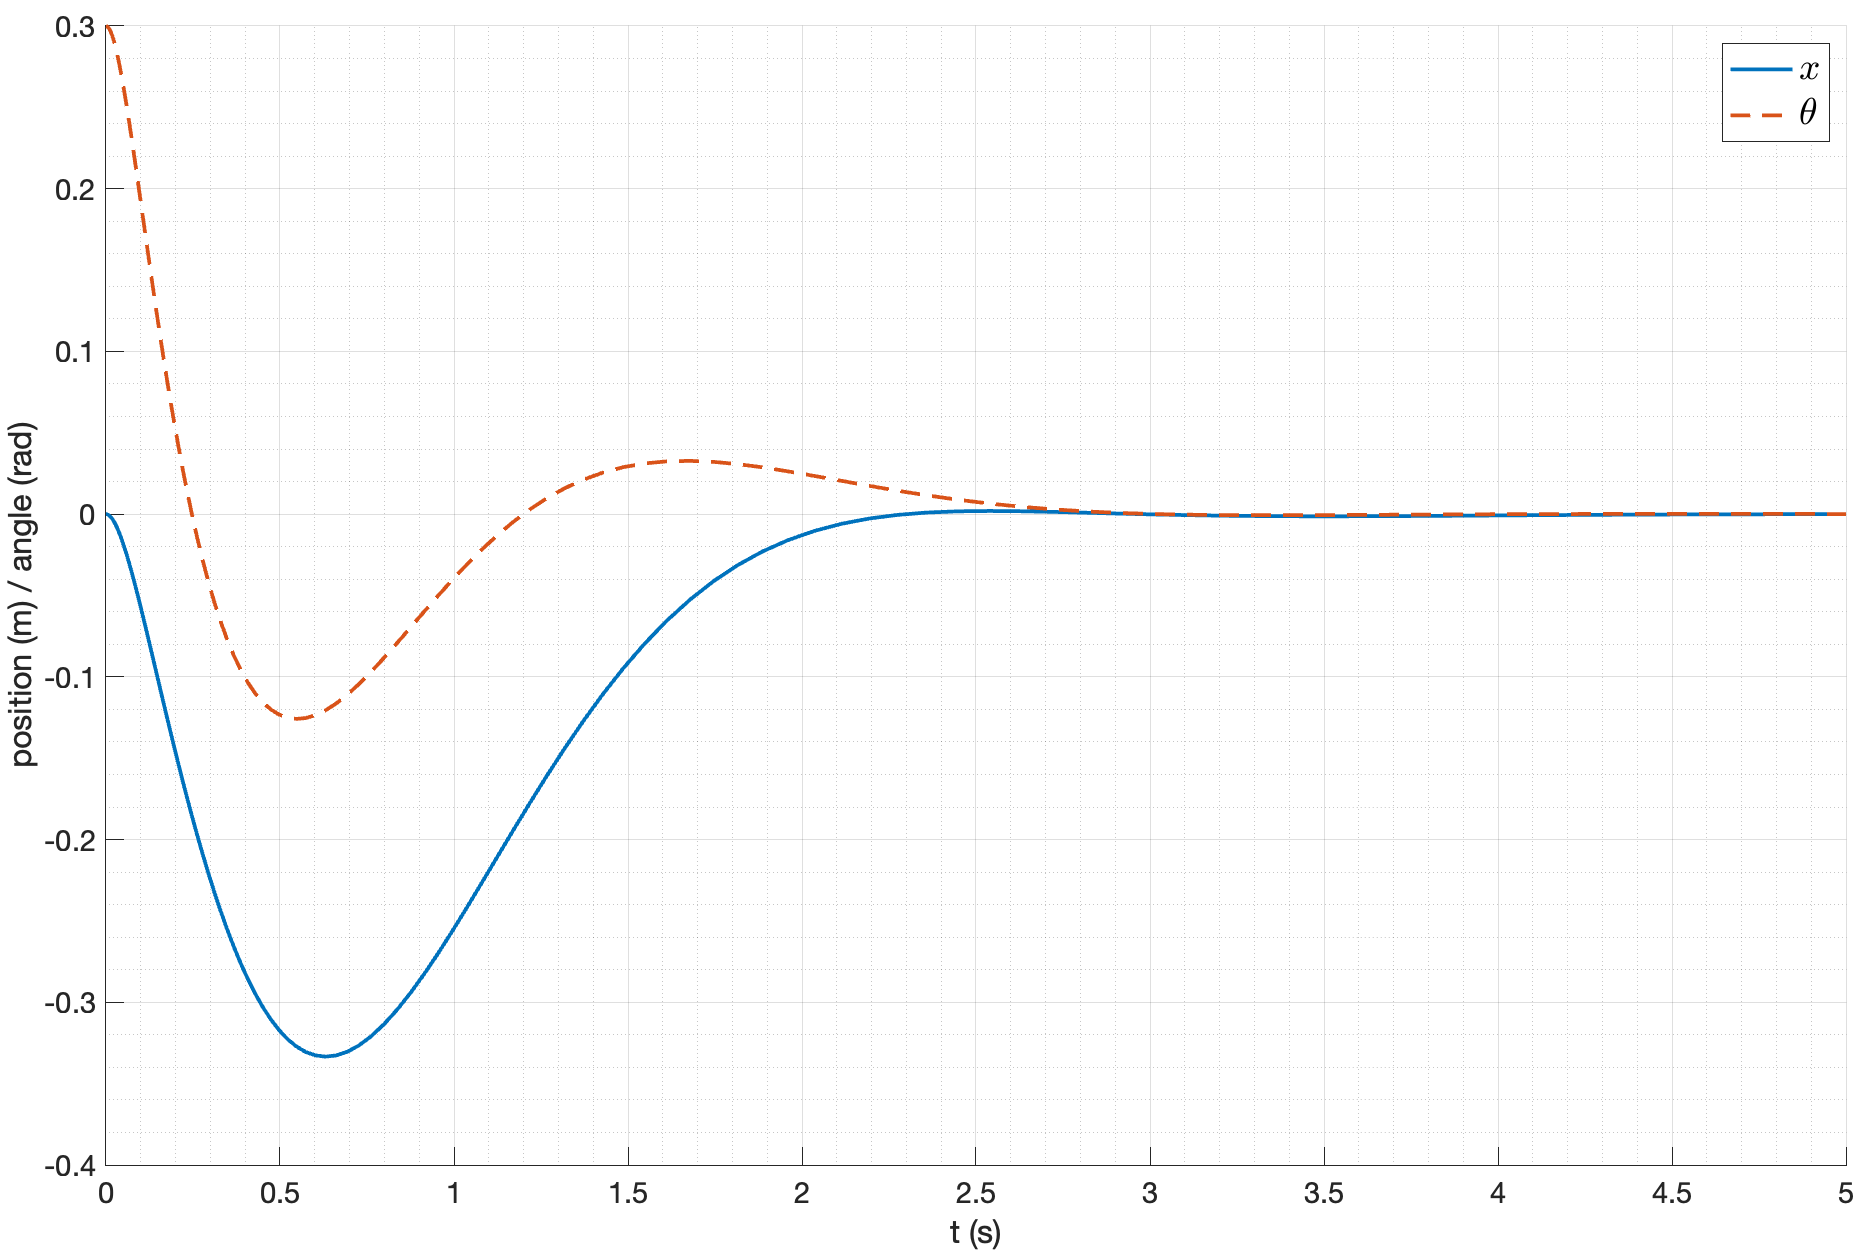
\includegraphics[width=0.8\textwidth]{media/plots/modal_controllers/out_1.png}
    \caption{Результаты моделирования нелинейной модели системы с модальным регулятором при $k = -4$}
    \label{fig:modal_controlers_1_out}
\end{figure}
\begin{figure}[ht!]
    \centering
    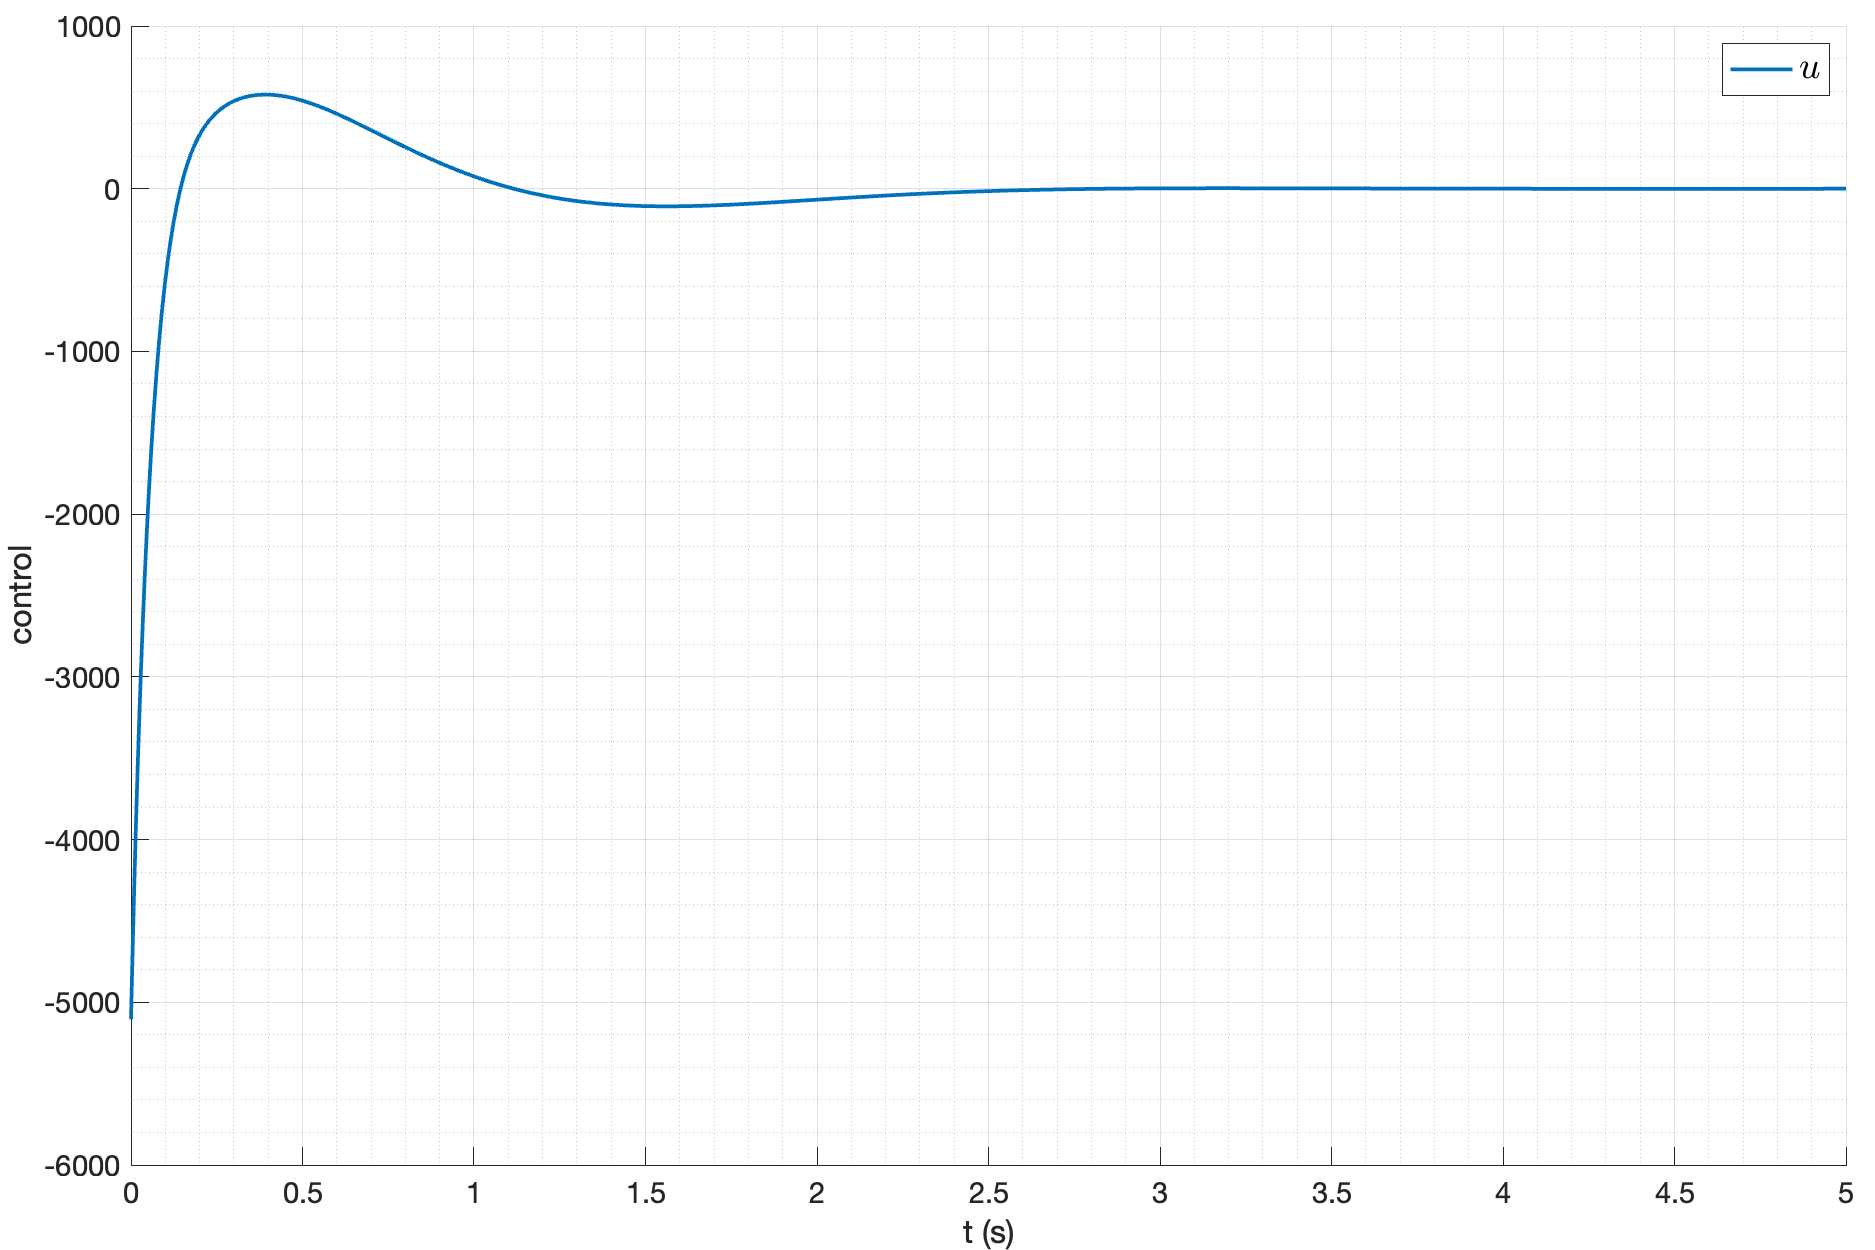
\includegraphics[width=0.8\textwidth]{media/plots/modal_controllers/u_1.png}
    \caption{Управляющее воздействие нелинейной модели системы с модальным регулятором при $k = -4$}
    \label{fig:modal_controlers_1_u}
\end{figure}
\begin{figure}[ht!]
    \centering
    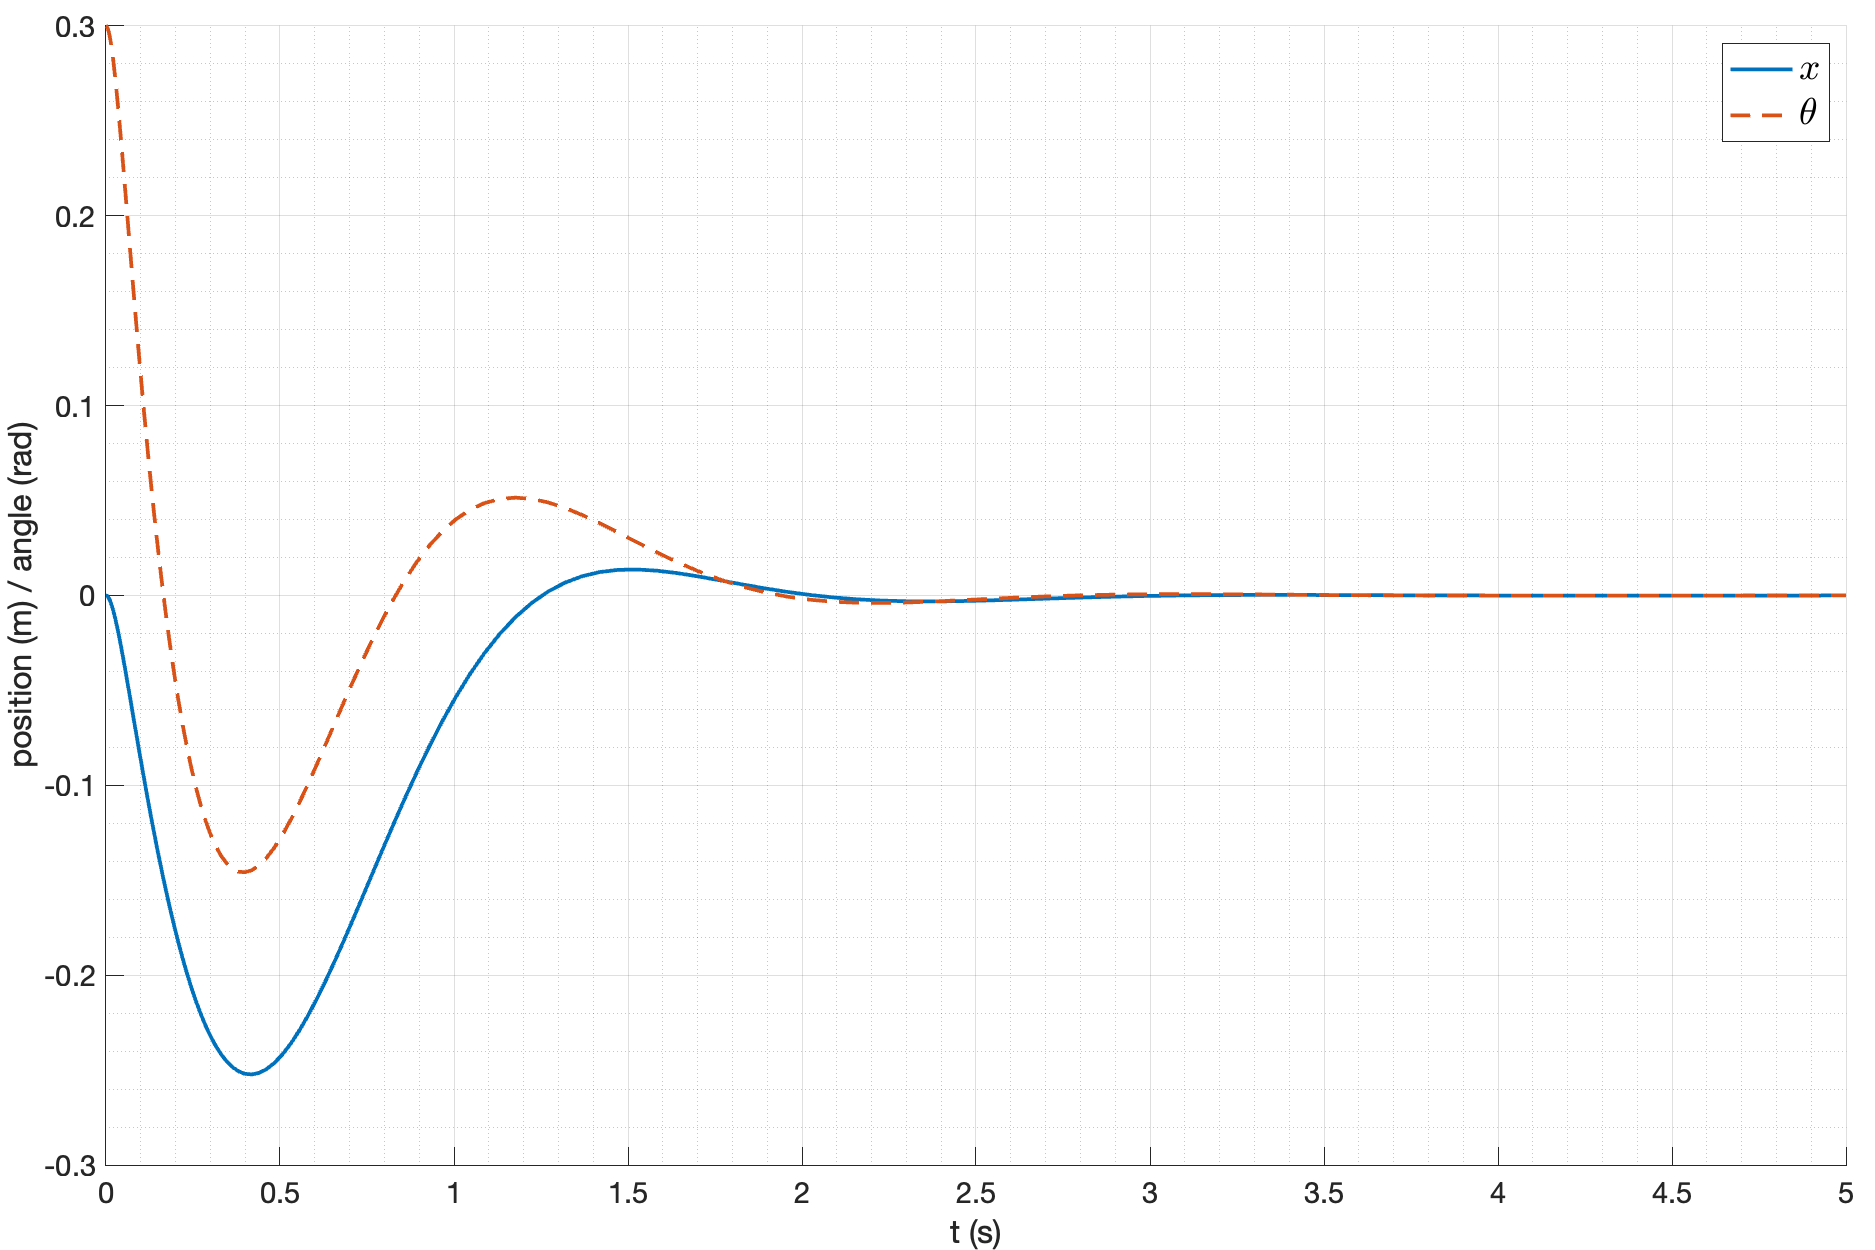
\includegraphics[width=0.8\textwidth]{media/plots/modal_controllers/out_2.png}
    \caption{Результаты моделирования нелинейной модели системы с модальным регулятором при $k = -6$}
    \label{fig:modal_controlers_2_out}
\end{figure}
\begin{figure}[ht!]
    \centering
    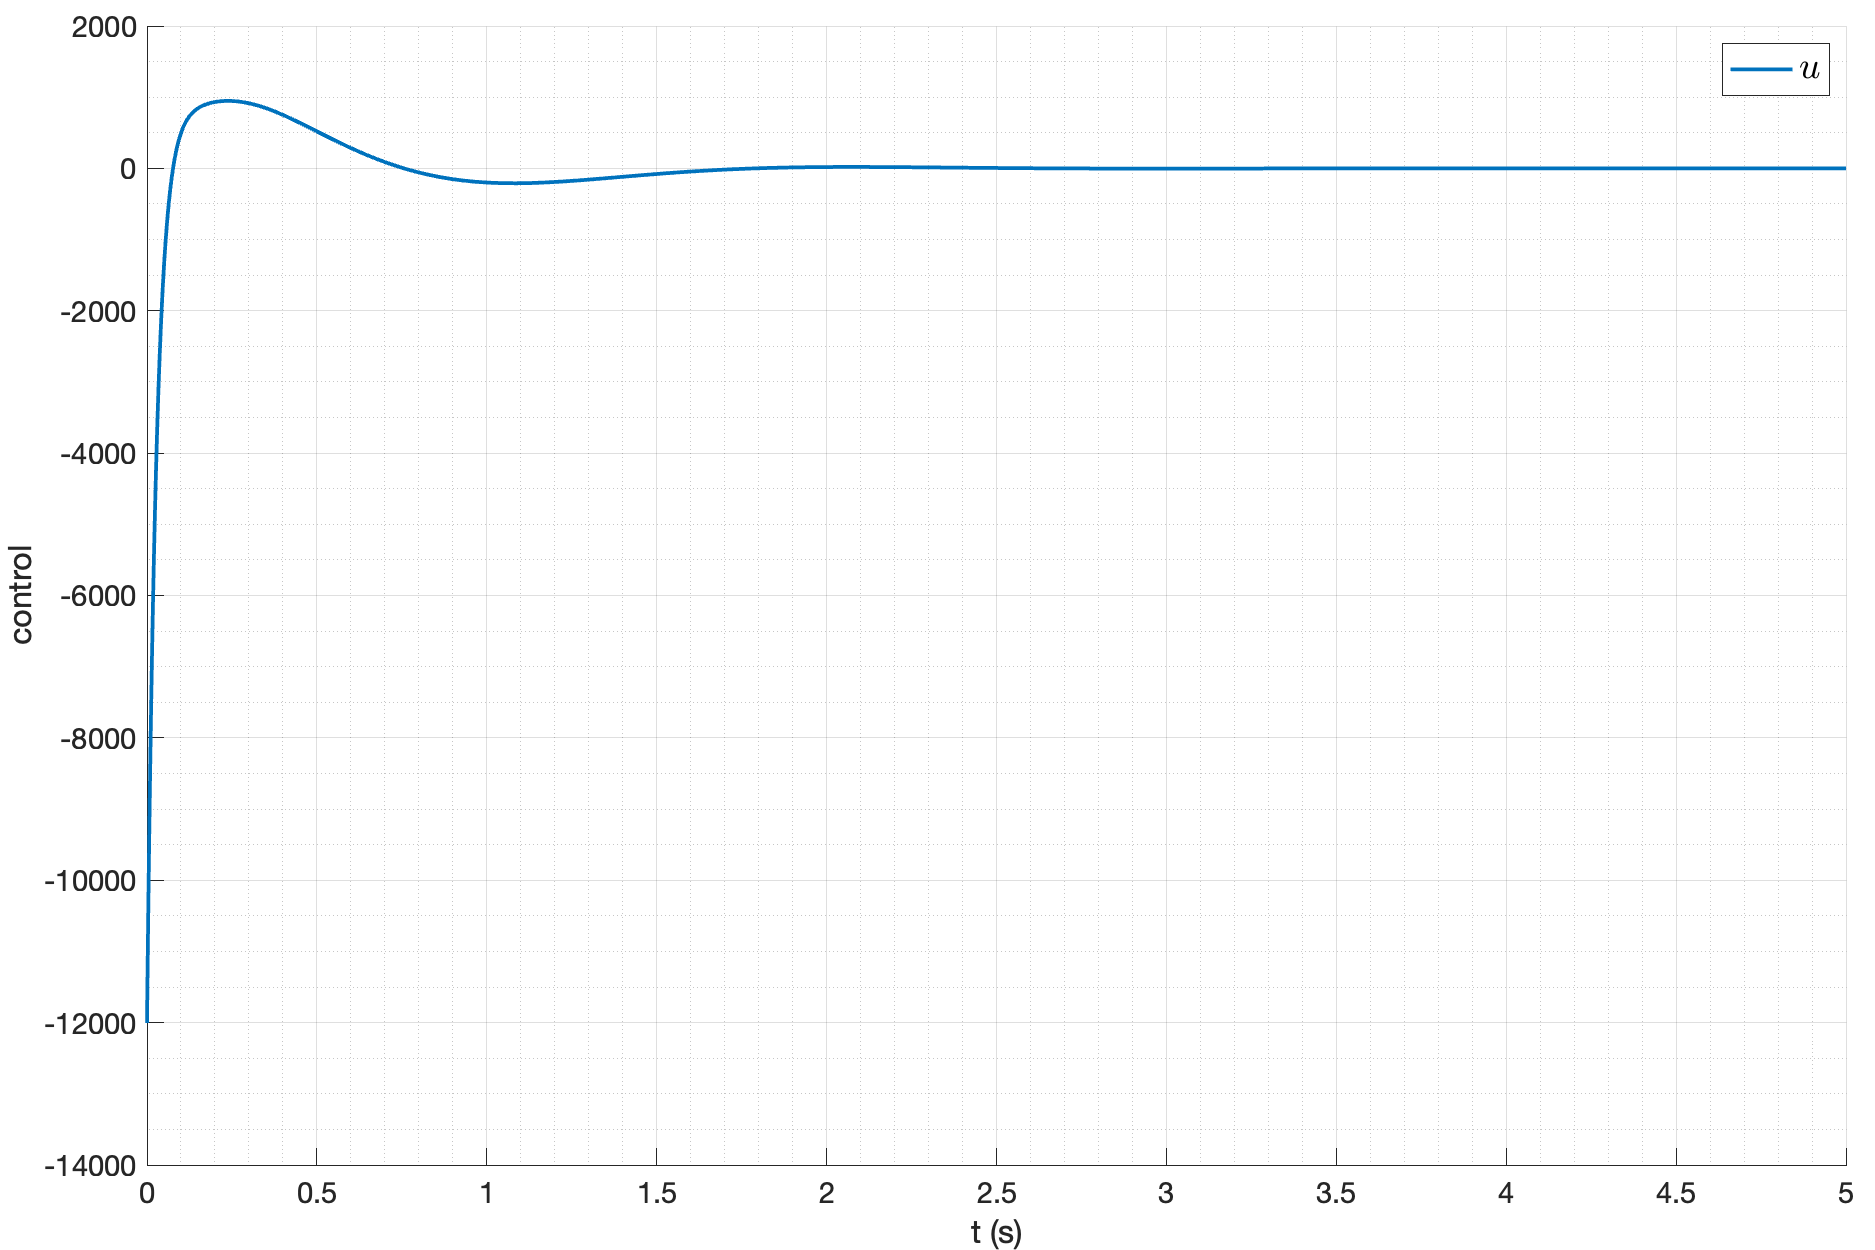
\includegraphics[width=0.8\textwidth]{media/plots/modal_controllers/u_2.png}
    \caption{Управляющее воздействие нелинейной модели системы с модальным регулятором при $k = -6$}
    \label{fig:modal_controlers_2_u}
\end{figure}
\begin{figure}[ht!]
    \centering
    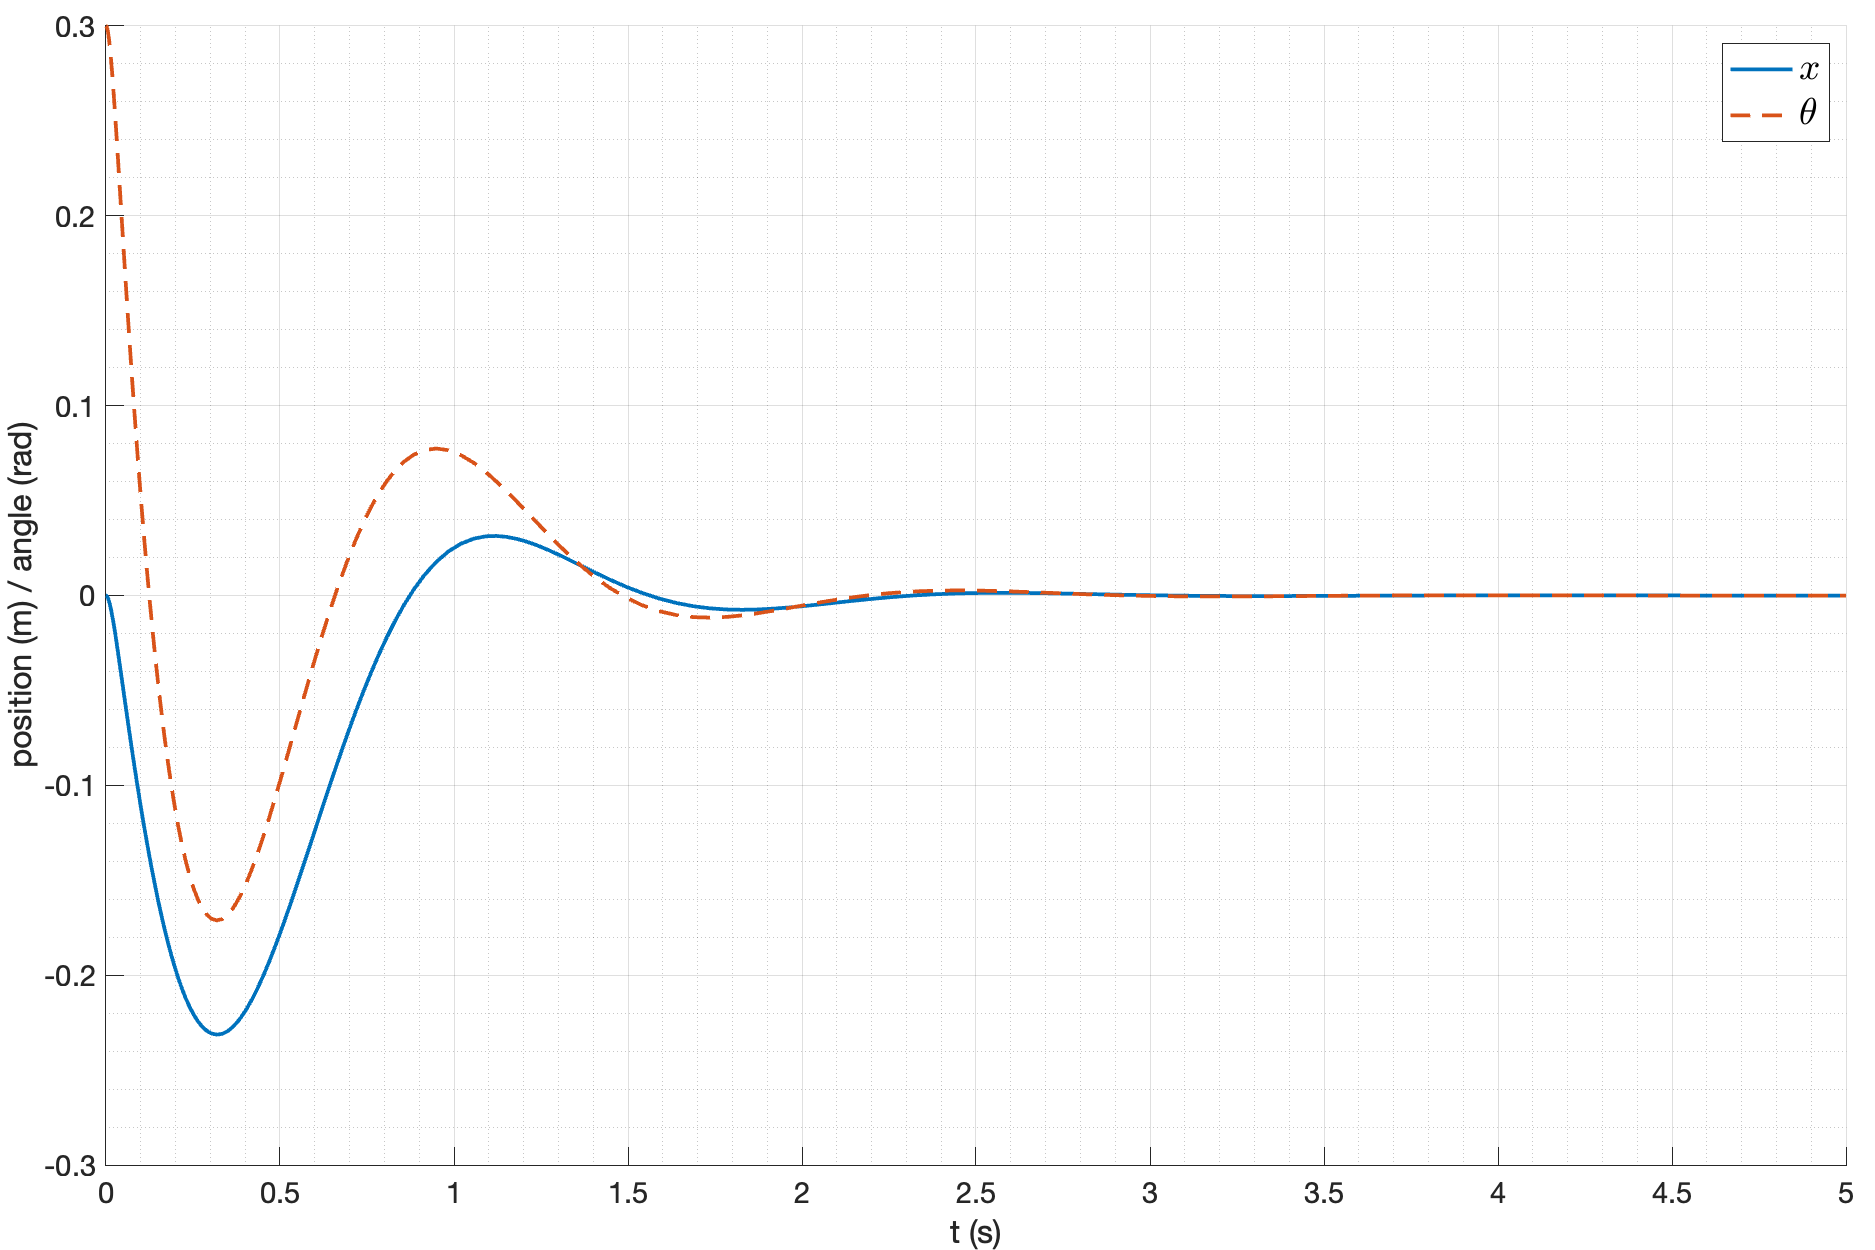
\includegraphics[width=0.8\textwidth]{media/plots/modal_controllers/out_3.png}
    \caption{Результаты моделирования нелинейной модели системы с модальным регулятором при $k = -8$}
    \label{fig:modal_controlers_3_out}
\end{figure}
\begin{figure}[ht!]
    \centering
    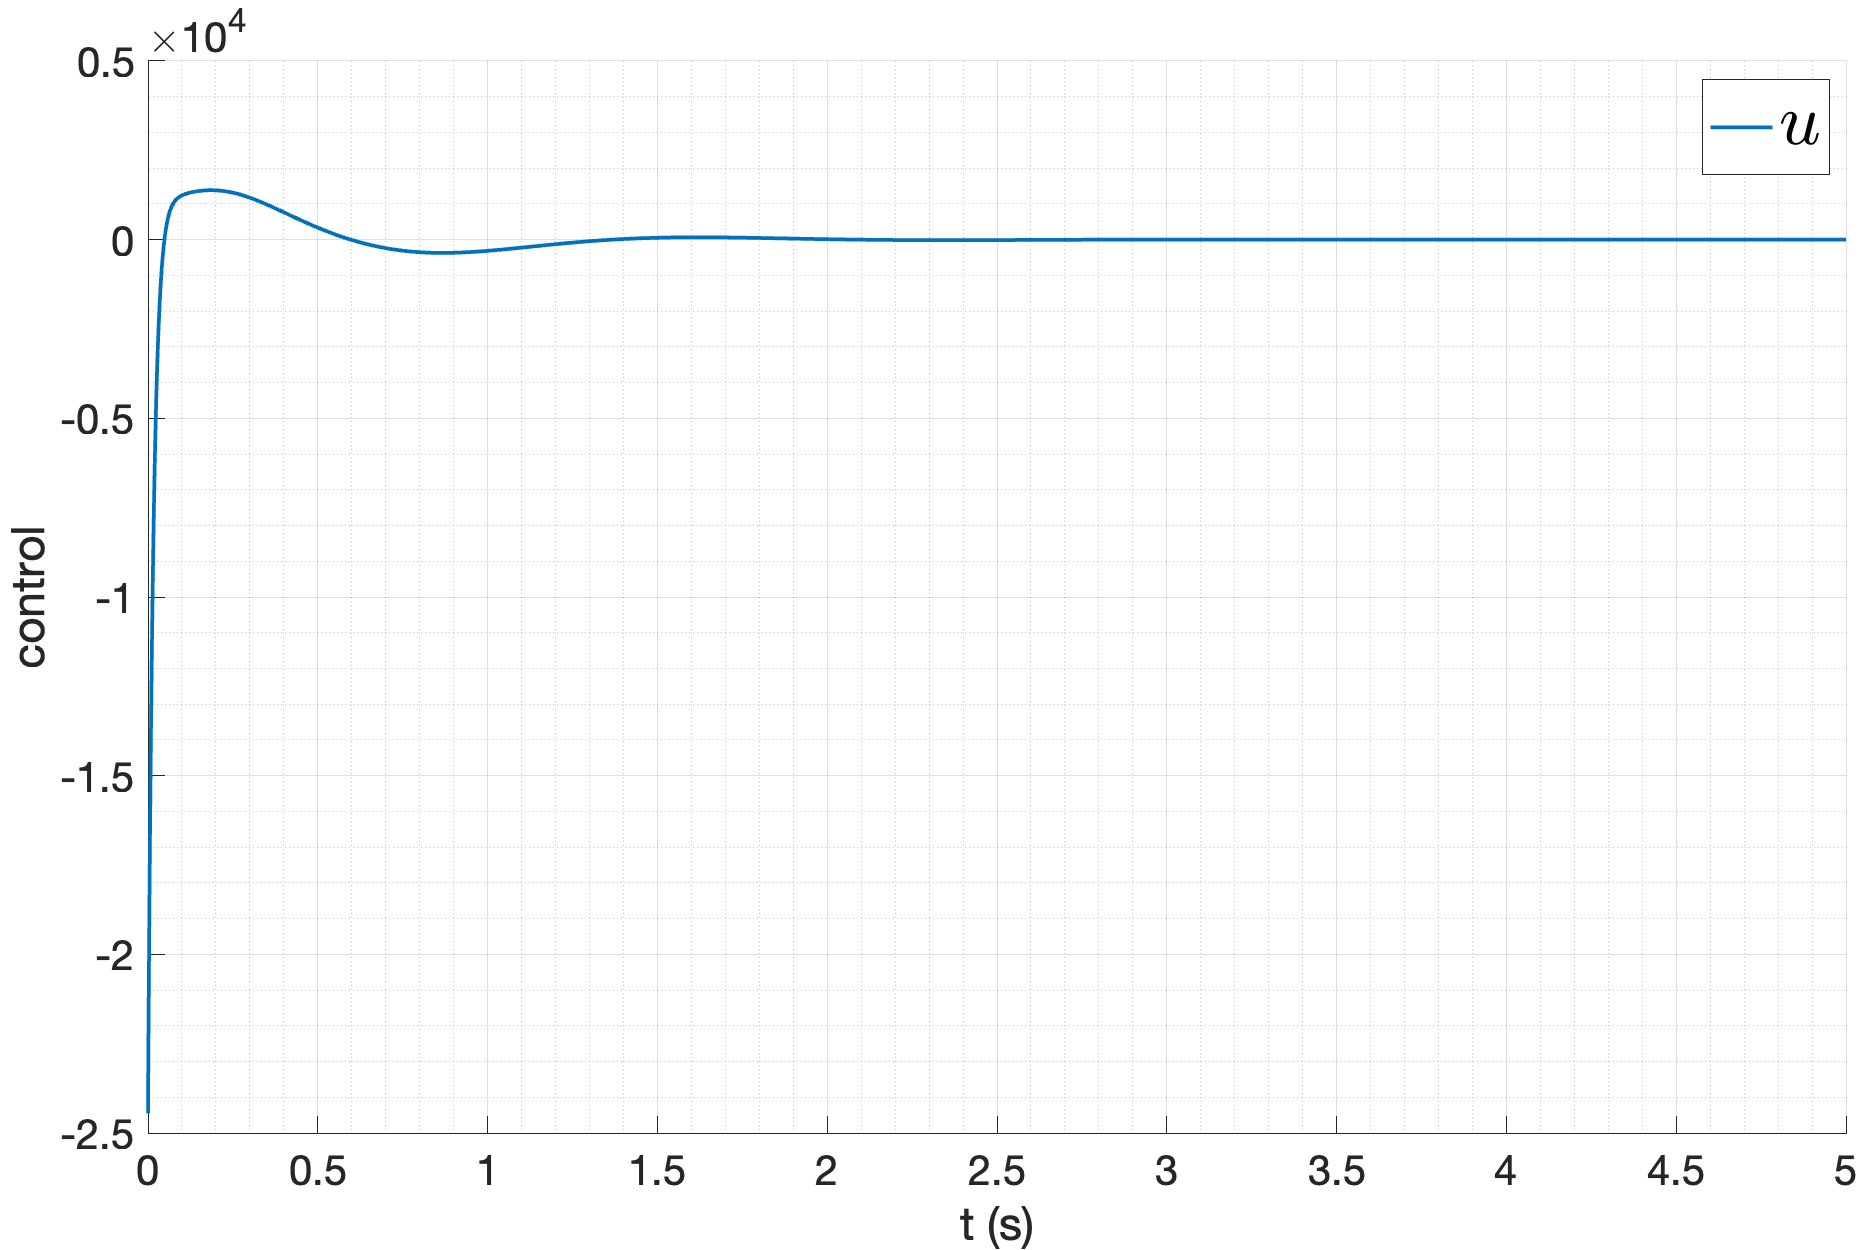
\includegraphics[width=0.8\textwidth]{media/plots/modal_controllers/u_3.png}
    \caption{Управляющее воздействие нелинейной модели системы с модальным регулятором при $k = -8$}
    \label{fig:modal_controlers_3_u}
\end{figure}
\begin{figure}[ht!]
    \centering
    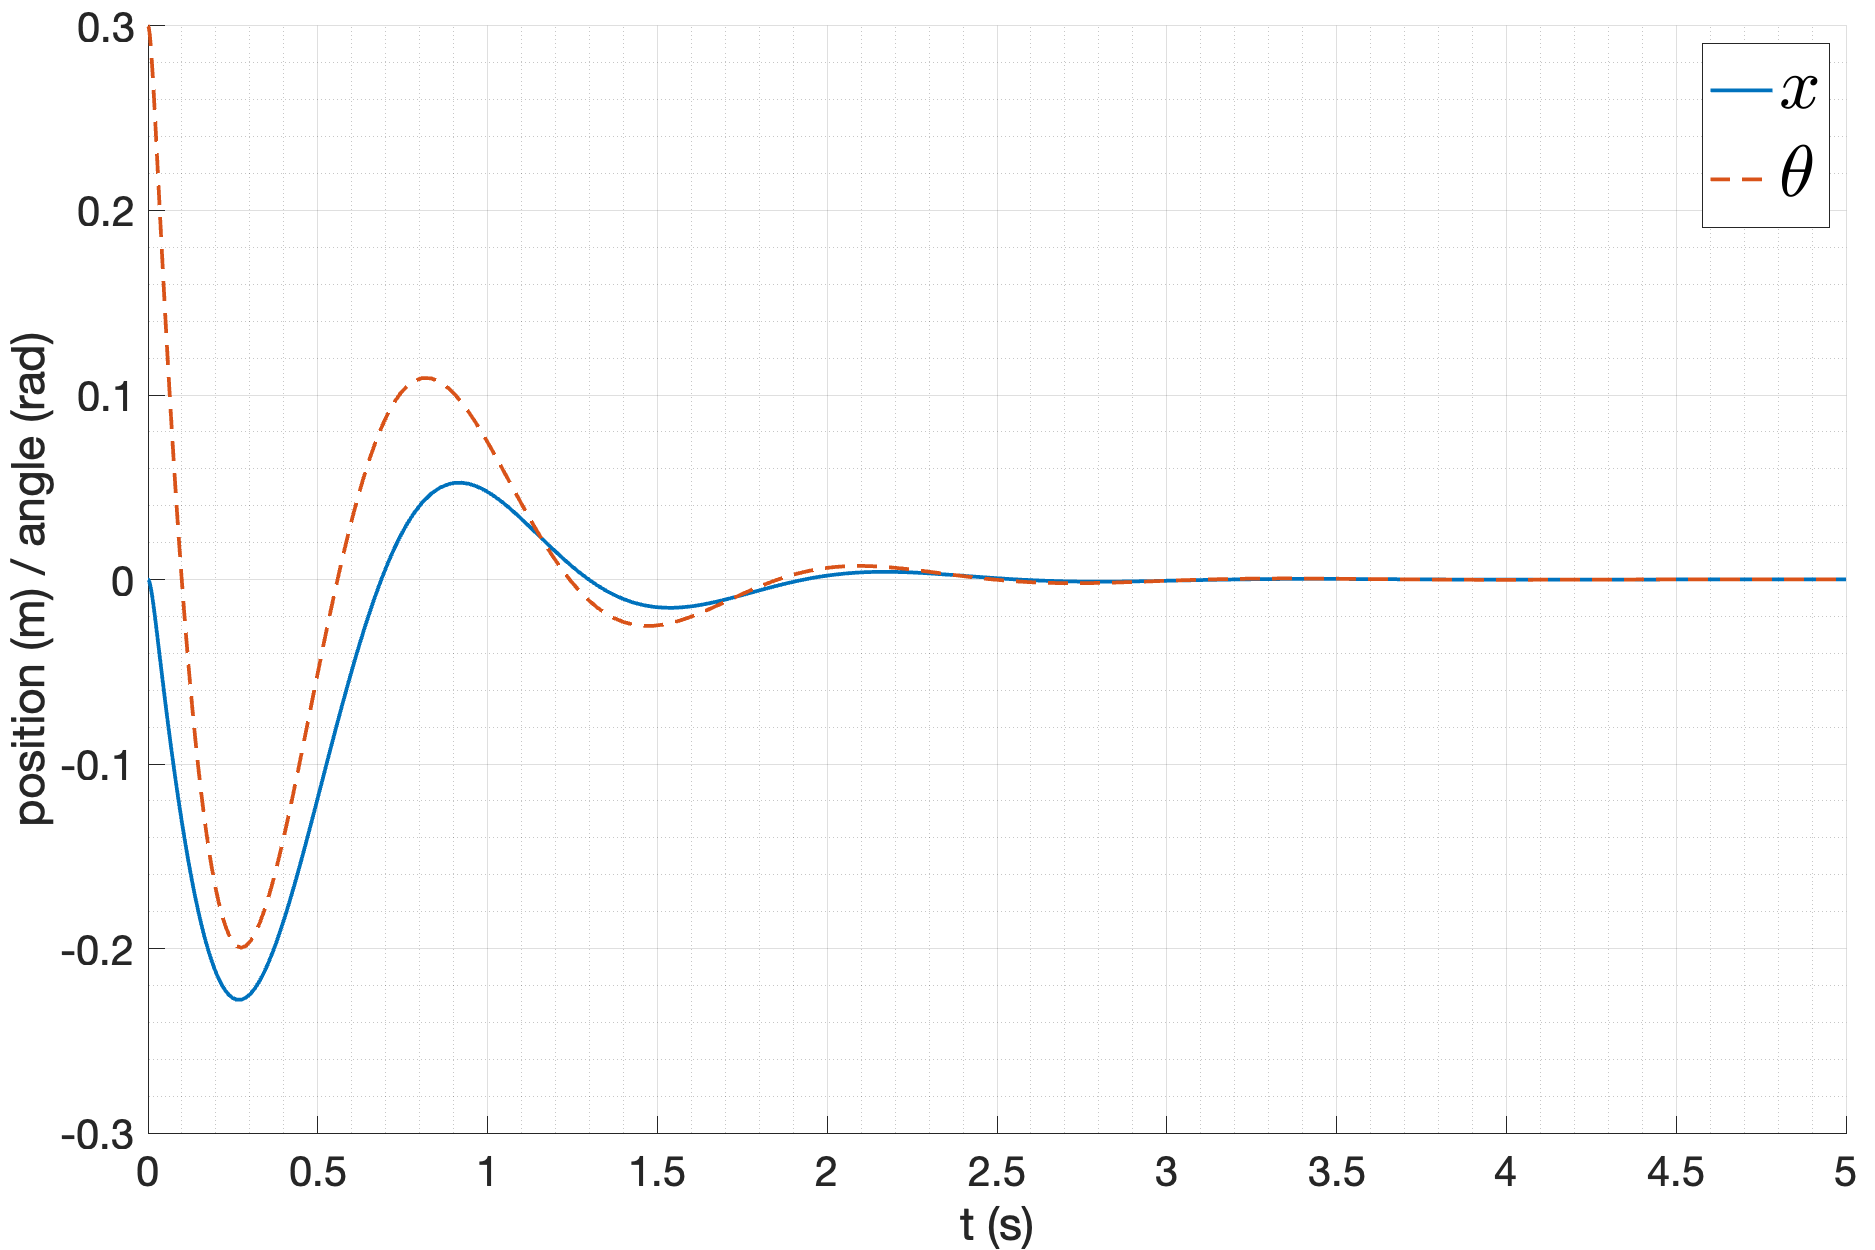
\includegraphics[width=0.8\textwidth]{media/plots/modal_controllers/out_4.png}
    \caption{Результаты моделирования нелинейной модели системы с модальным регулятором при $k = -10$}
    \label{fig:modal_controlers_4_out}
\end{figure}
\begin{figure}[ht!]
    \centering
    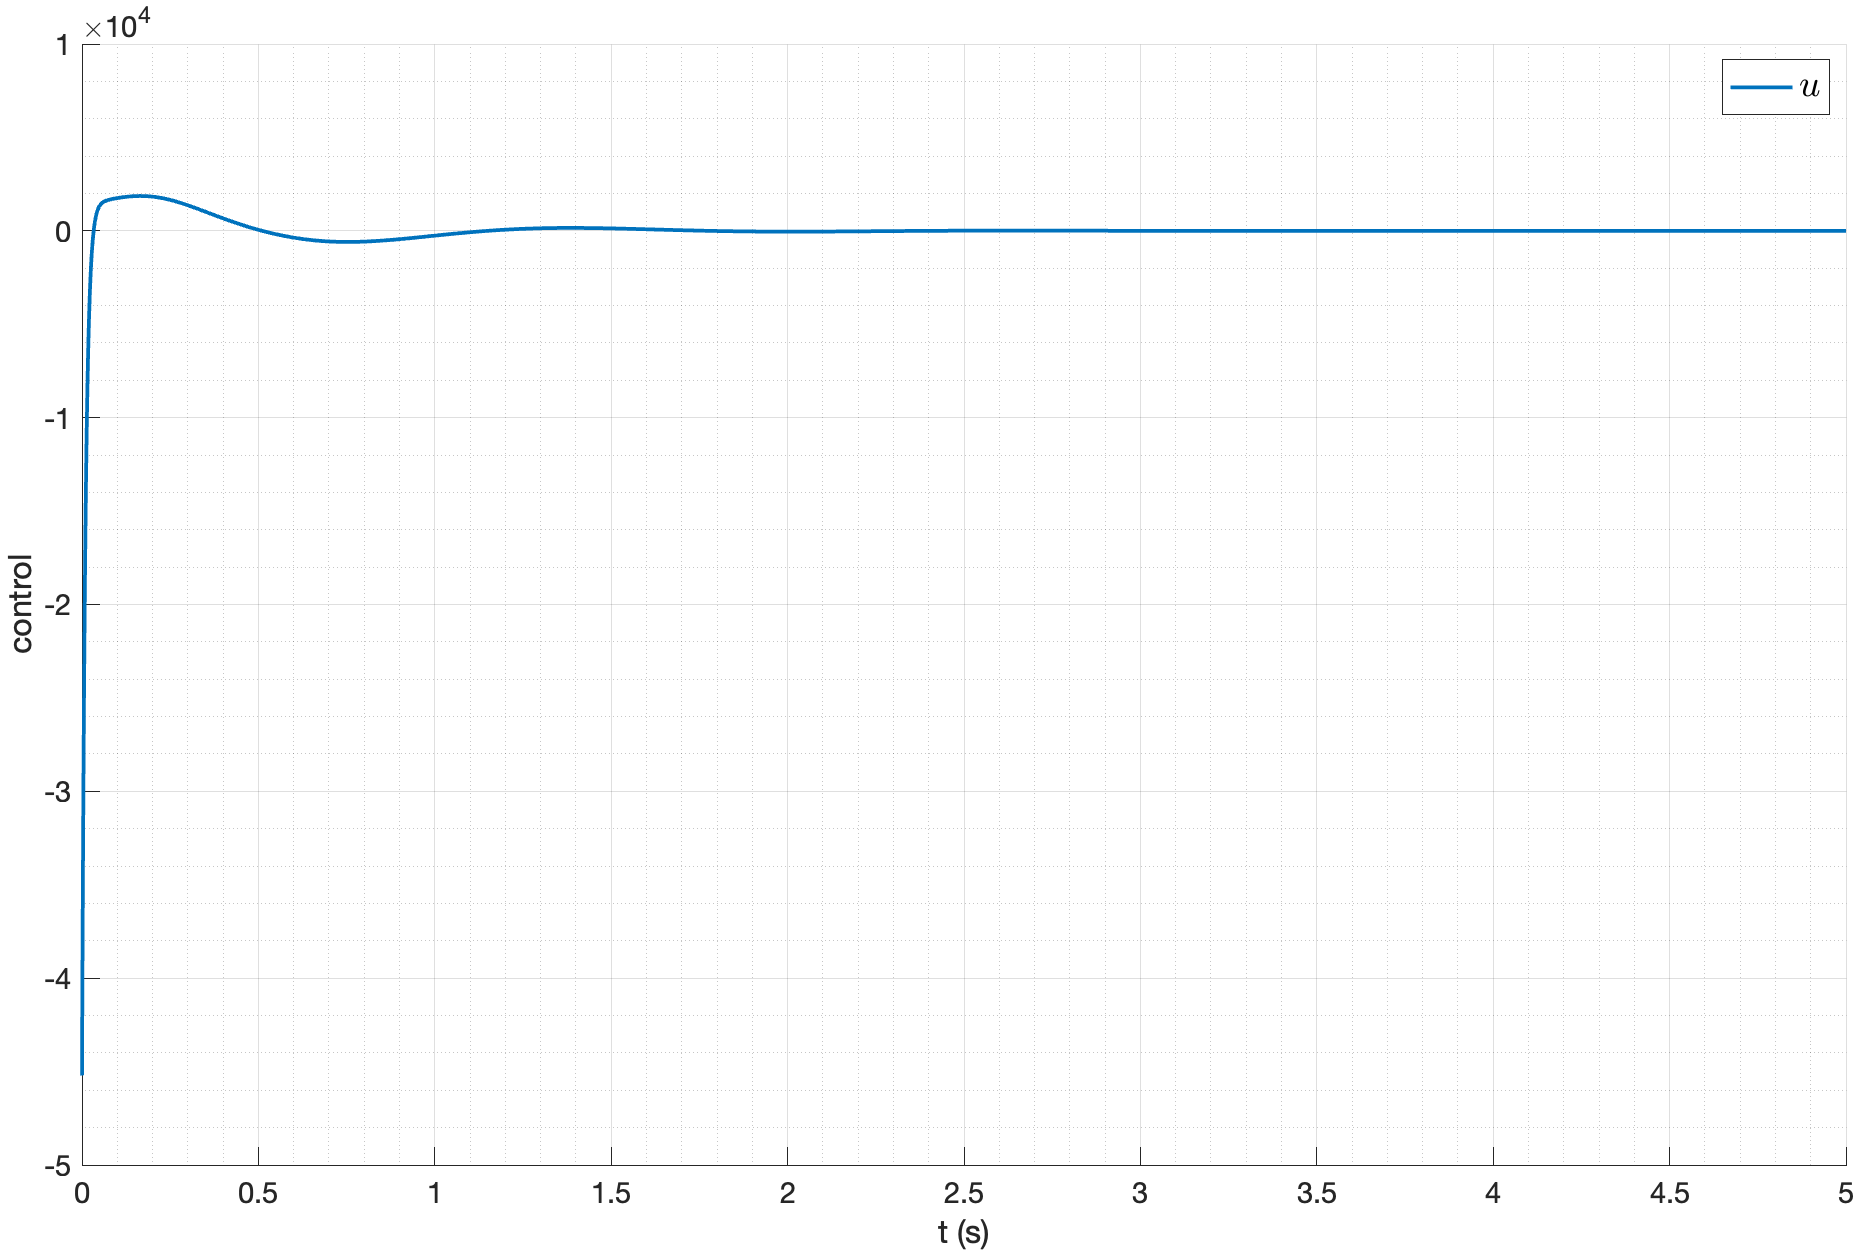
\includegraphics[width=0.8\textwidth]{media/plots/modal_controllers/u_4.png}
    \caption{Управляющее воздействие нелинейной модели системы с модальным регулятором при $k = -10$}
    \label{fig:modal_controlers_4_u}
\end{figure}
Можно заметить, что при увеличении модуля собственных чисел замкнутой системы, время переходного процесса
сокращается, а перегулирование отклонения маятника увеличивается, максимальный модуль управляющего воздействия 
тоже увеличивается с увеличением модуля собственных чисел. Численные результаты сравнения приведены в таблице \ref{tab:modal_control_cmp}. 

\begin{table}[ht!]
    \centering
    \begin{tabular}{|c|c|c|c|c|}
        \hline
        $k$ & $t_{\text{set}}$, с & $M_{\theta}$ & $M_{x}$ & $\max{|u|}$ \\
        \hline
        -4 & 2.9 & 0.11 & 0.34 & 5100 \\
        \hline
        -6 & 2.7 & 0.16 & 0.26 & 12000 \\
        \hline
        -8 & 2.5 & 0.18 & 0.24 & 24000 \\
        \hline
        -10 & 1.4 & 0.2 & 0.23 & 44000 \\
        \hline
    \end{tabular}
    \caption{Сравнение регуляторов с различными собственными числами замкнутой системы}
    \label{tab:modal_control_cmp}
\end{table}

Можно заметить, что перегулирование координаты тележки остается практически одинаковым, 
что связано с тем, что угол маятника зависит от скорости и ускорения тележки, а не от ее положения. 

\FloatBarrier
Дополнительно посмотрим на случай замкнутой системы, имеющий спектр $\begin{bmatrix}-0.5 & -0.5 & -4 &- 4\end{bmatrix}$
и сравним ее с системой, имеющей спектр $\begin{bmatrix}-4 & -4 & -4 &- 4\end{bmatrix}$, рассмотренной на рисунке \ref{fig:modal_controlers_1_out}.
Графики результатов моделирования приведены на рисунке \ref{fig:modal_controlers_5_out} -- \ref{fig:modal_controlers_5_u}. 
\begin{figure}[ht!]
    \centering
    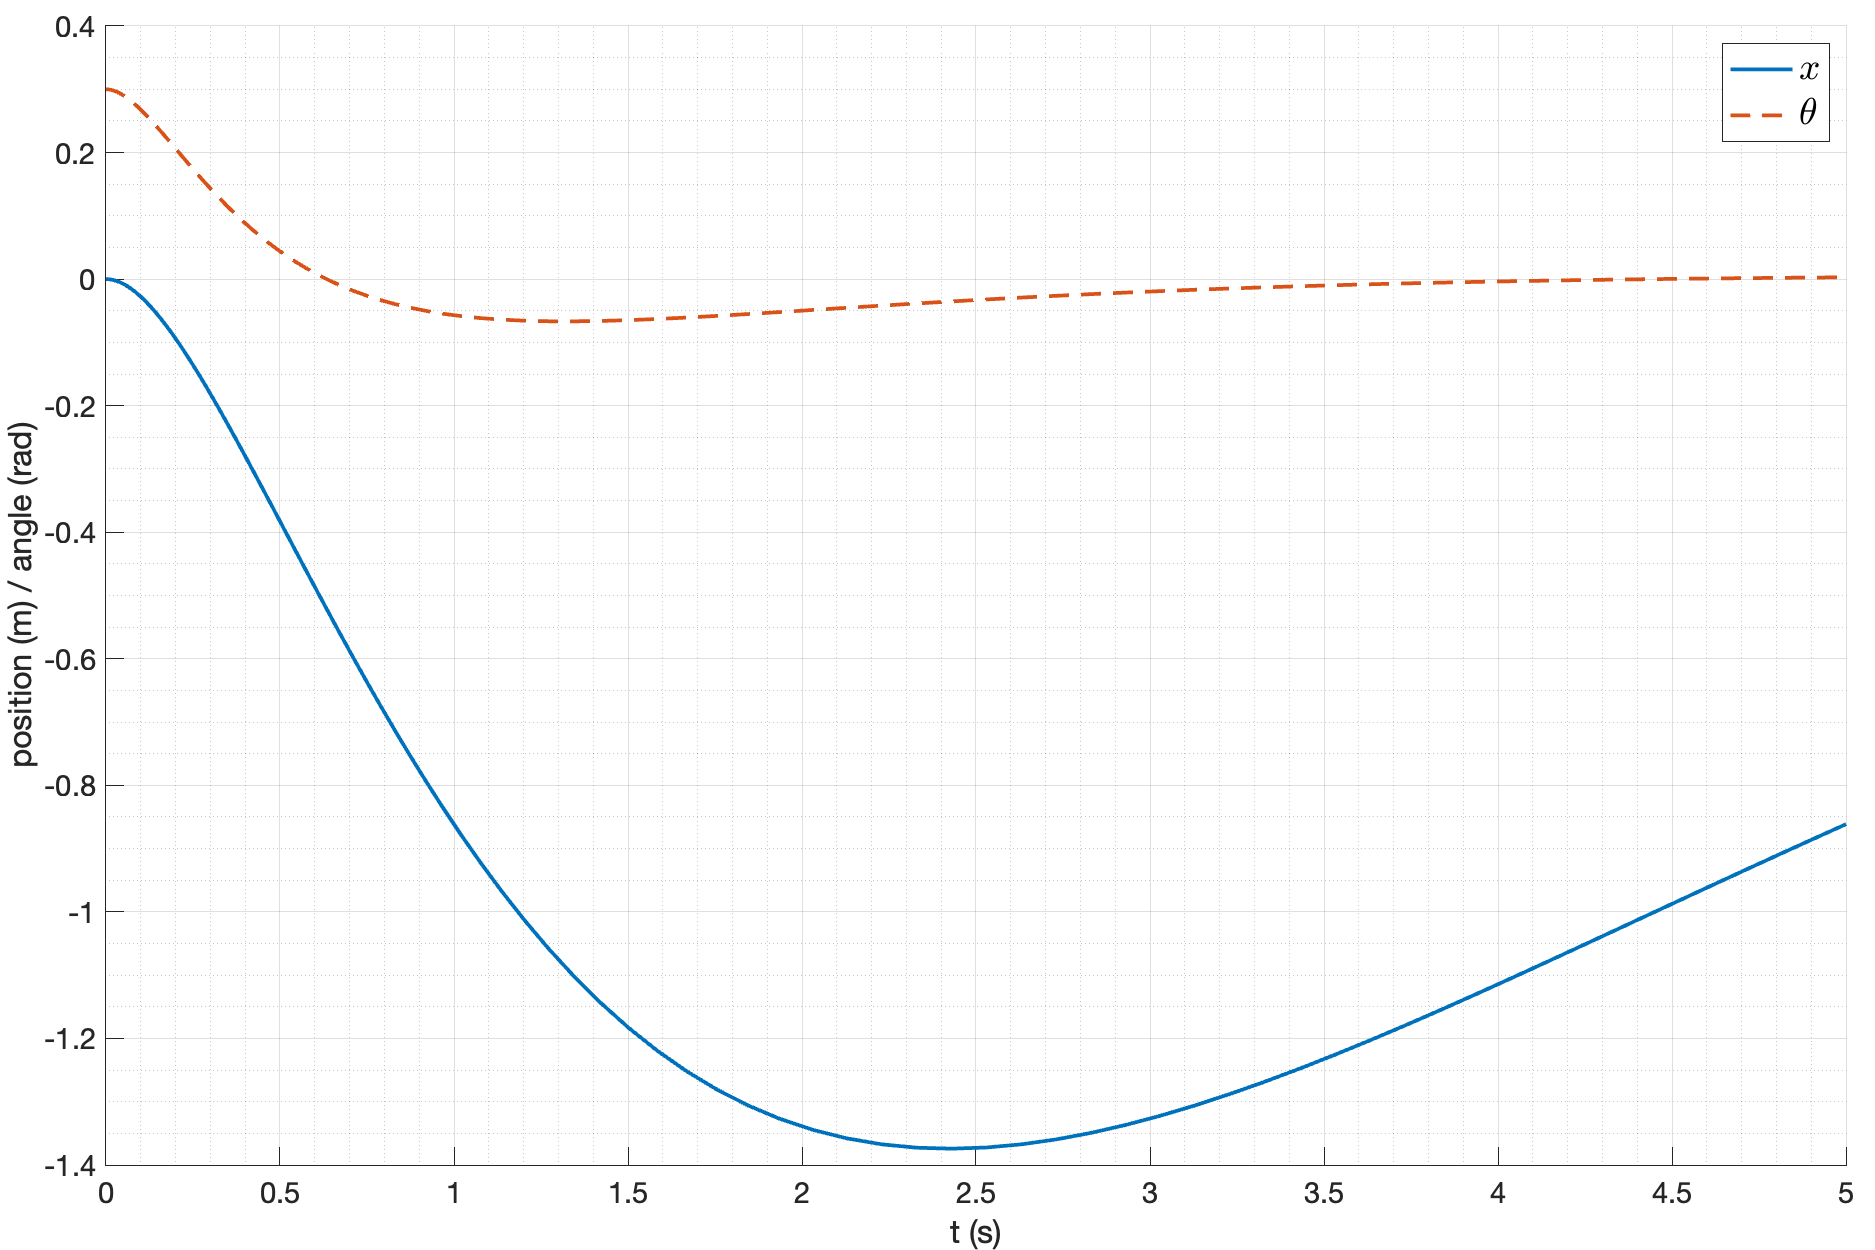
\includegraphics[width=0.8\textwidth]{media/plots/modal_controllers/out_5.png}
    \caption{Результаты моделирования нелинейной модели системы со спектром $\begin{bmatrix}-0.5 & -0.5 & -4 &- 4\end{bmatrix}$}
    \label{fig:modal_controlers_5_out}
\end{figure}
\begin{figure}[ht!]
    \centering
    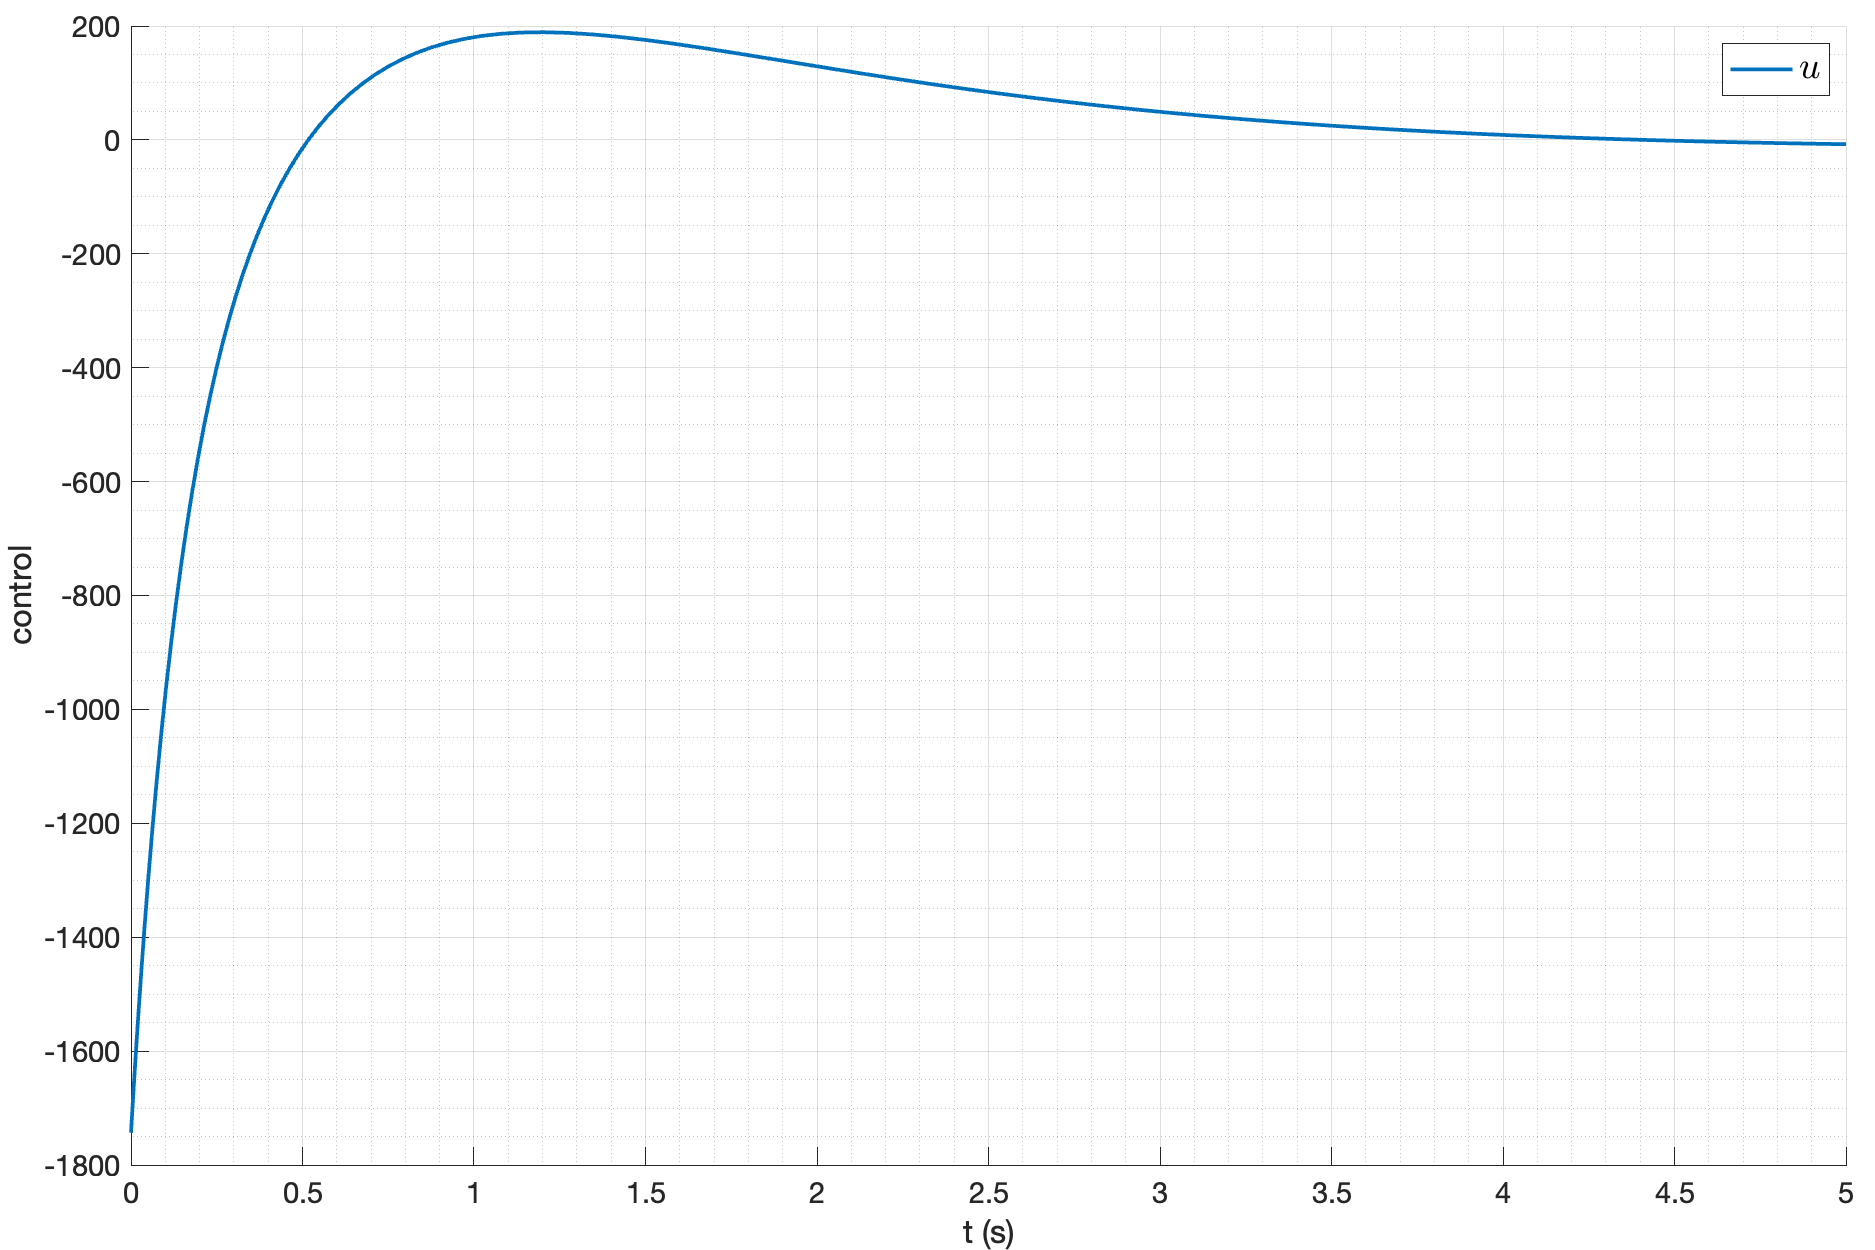
\includegraphics[width=0.8\textwidth]{media/plots/modal_controllers/u_5.png}
    \caption{Управляющее воздействие нелинейной модели системы со спектром $\begin{bmatrix}-0.5 & -0.5 & -4 &- 4\end{bmatrix}$}
    \label{fig:modal_controlers_5_u}
\end{figure}
\FloatBarrier
Видно, что при уменьшении первых двух собственных чисел замкнутой системы, время переходного процесса для 
координаты тележки сильно увеличивается, а для угла отклонения маятника практически не меняется, при этом 
управление тоже становится меньше. При уменьшении первых двух собственных чисел произошло влияние на первые 
два собственные вектора системы (\ref{eq:eigenvectors}), которые, в свою очередь, влияют на 
линейное положение тележки, но не на угол отклонения маятника. Таким образом, можно сделать вывод, что 
с использованием модального управления можно влиять на динамику системы \textit{по отдельности}, изменяя 
собственные числа для каждого из собственных векторов.

\subsection{Наблюдатель полного порядка}
Рассмотрим наблюдатель полного порядка, основанный на линейной модели системы: 
\begin{equation}
    \begin{cases}
        \dot{\hat{x}} = A\hat{x} + Bu + L(y - C\hat{x})\\
        \hat{y} = C\hat{x}
    \end{cases}
\end{equation}
где $L$ -- матрица коррекции наблюдателя. 

Для синтеза наблюдателя воспользуемся уравнением Сильвестра, решение которого будем находить с помощью
пакета \texttt{cvx} в MATLAB.
\begin{equation}
    \begin{cases}
        \Gamma Q - QA = YC \\ 
        L = QY^{-1}
    \end{cases}
\end{equation}
где $\Gamma$ -- матрица с желаемыми собственными числами. 

Синтезируем наблюдатель с желаемым спектром $\{-3, -3, -3, -3\}$. 
Решим уравнение Сильвестра с помощью пакета \texttt{cvx} в MATLAB, в результате получаем матрицу наблюдателя $L$:
\begin{equation}
    L = \begin{bmatrix}
    5.30  & 5.30 \\ 
    3.20  & 3.20 \\ 
    -17.30  & -17.30 \\ 
    -76.79  & -76.79 \\
    \end{bmatrix}
\end{equation}
Проверим правильность полученного результата, вычислив собственные числа замкнутой системы $A + LC$: 
\begin{equation}
    \sigma(A + LC) = \begin{bmatrix}
    -3.00 \\ 
    -3.00 \\ 
    -3.00 \\ 
    -3.00 \\ 
    \end{bmatrix}
\end{equation}
Проверим полученный наблюдатель, сравнив его выход с реальным состоянием нелинейной системы. В качестве регулятора 
выберем регулятор со спектром $\begin{bmatrix}-6 & -6 & -6 & -6\end{bmatrix}$, рассмотренный ранее. В качестве 
начальных условий возьмем $\theta_0 = 0.3$ для системы и $\hat{X}_0 = 0$ для наблюдателя.

Схема наблюдателя приведена на рисунке \ref{fig:observer_scheme}. Схема включения наблюдателя в систему 
показана на рисунке \ref{fig:observer_system}. 
\begin{figure}[ht!]
    \centering
    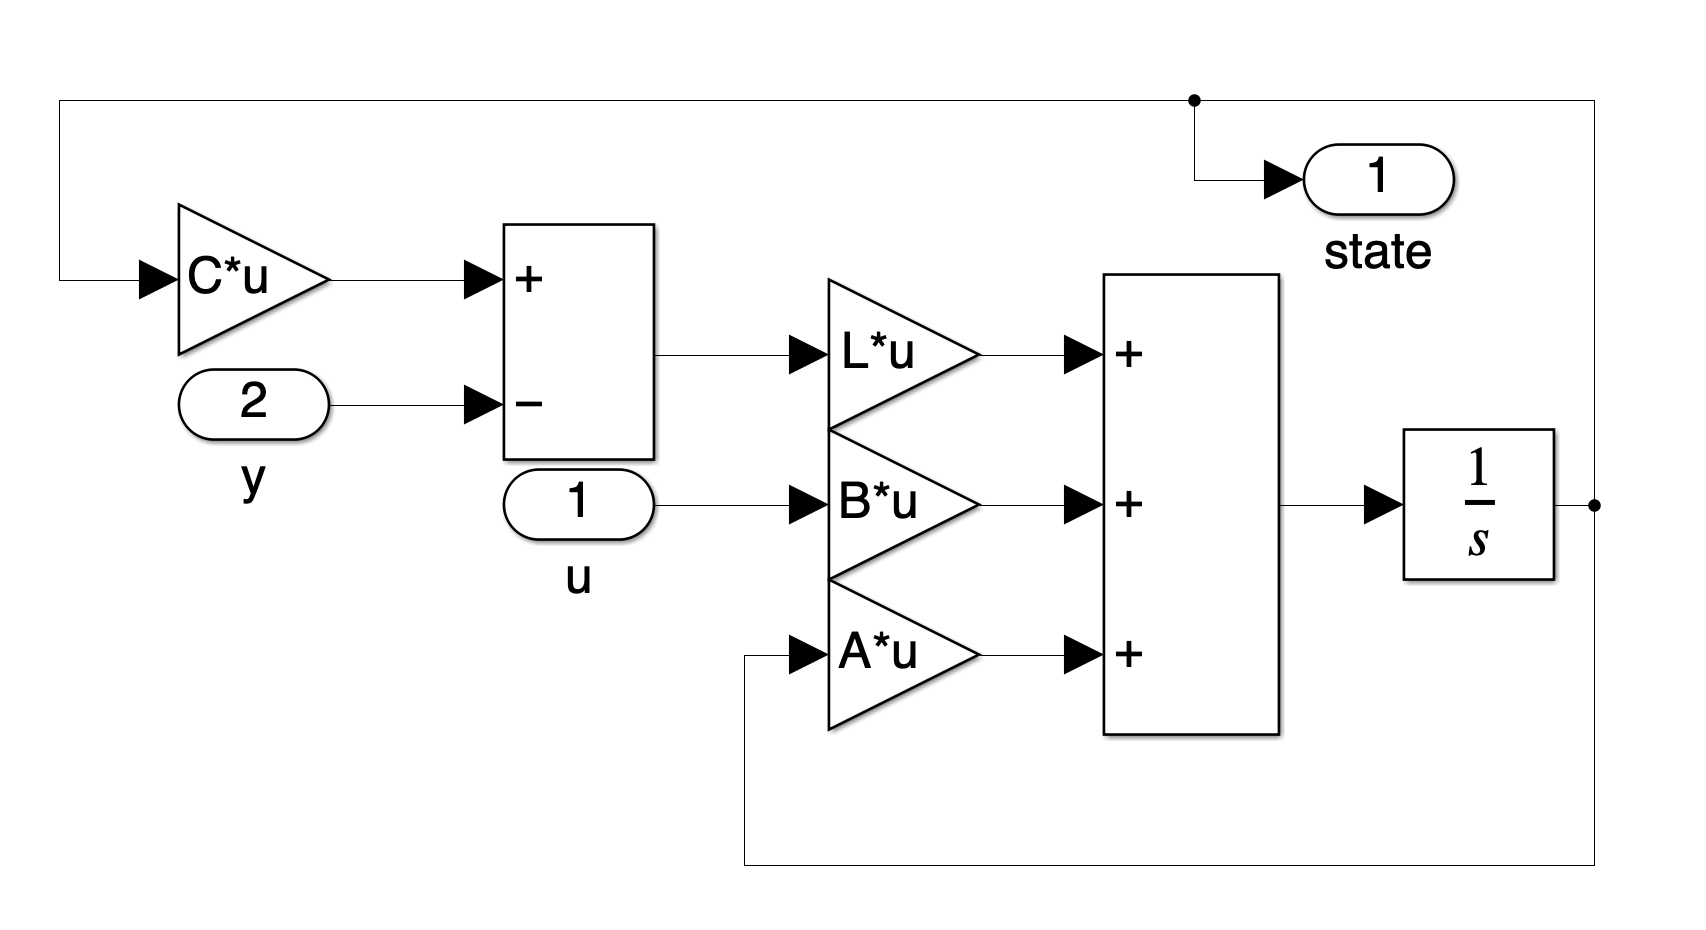
\includegraphics[width=0.7\textwidth]{media/observer_scheme.png}
    \caption{Схема наблюдателя}
    \label{fig:observer_scheme}
\end{figure}
\begin{figure}[ht!]
    \centering
    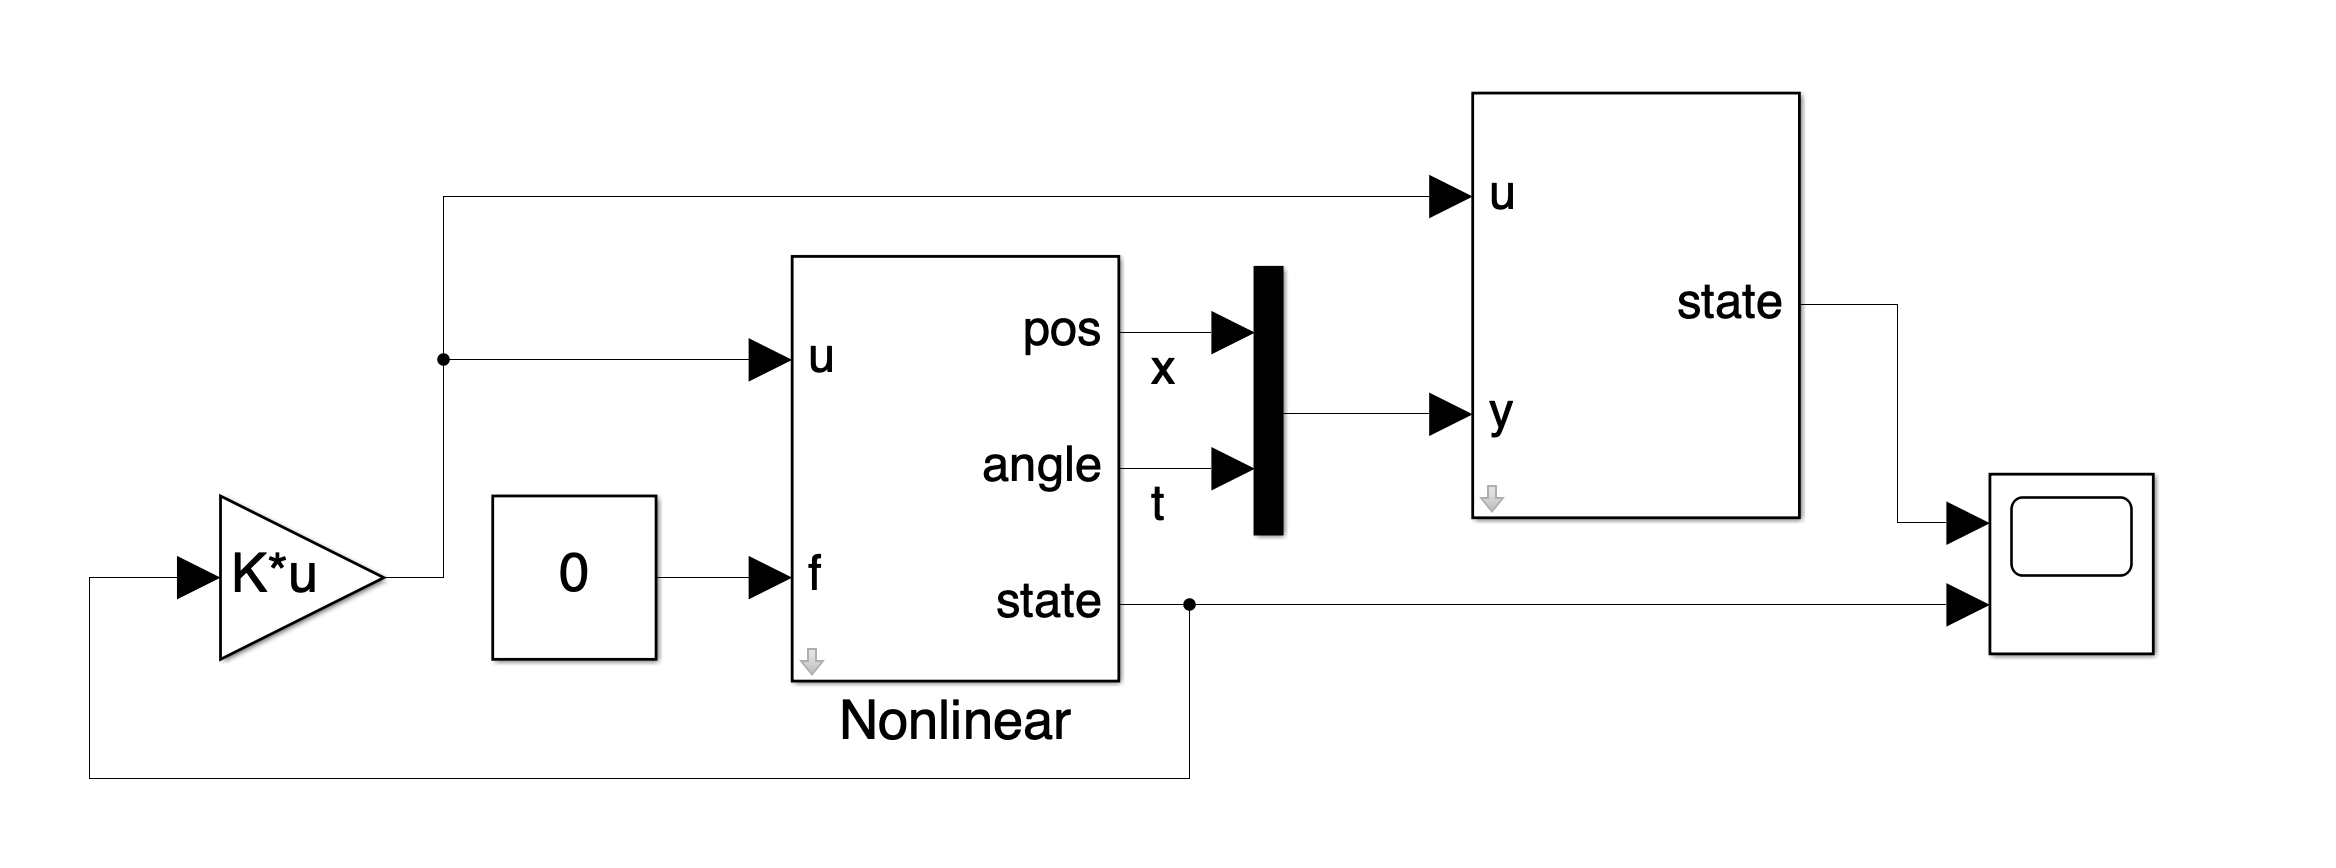
\includegraphics[width=0.7\textwidth]{media/observer_system.png}
    \caption{Схема включения наблюдателя в систему}
    \label{fig:observer_system}
\end{figure}

Результаты моделирования приведены на рисунке \ref{fig:observer_x_1} и рисунках \ref{fig:observer_x_cmp_1_sep}. 
\begin{figure}[ht!]
    \centering
    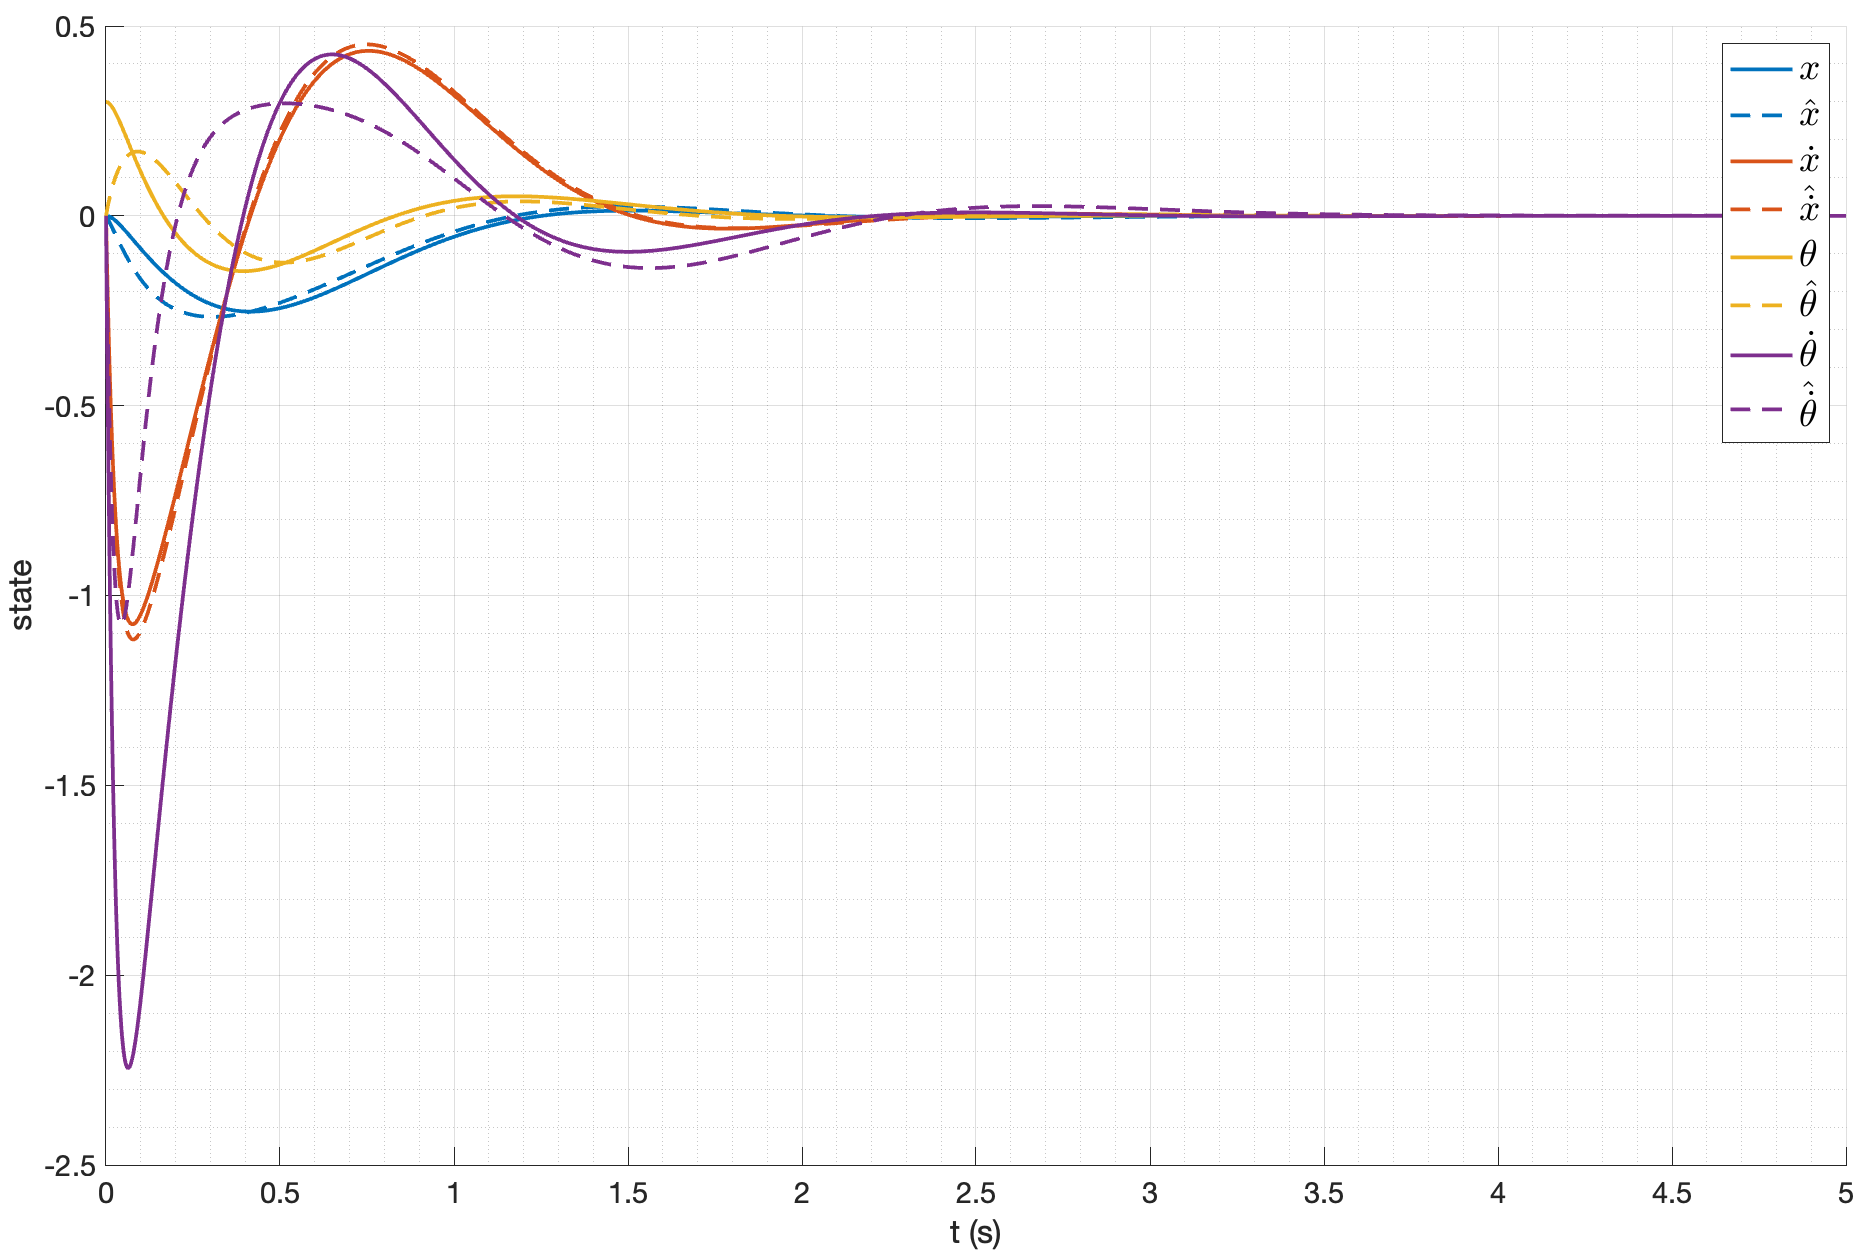
\includegraphics[width=\textwidth]{media/plots/modal_observer/observer_cmp_1.png}
    \caption{Результаты моделирования наблюдателя полного порядка}
    \label{fig:observer_x_1}
\end{figure}
\begin{figure}[ht!]
    \centering
    \begin{subfigure}[b]{0.45\textwidth}
        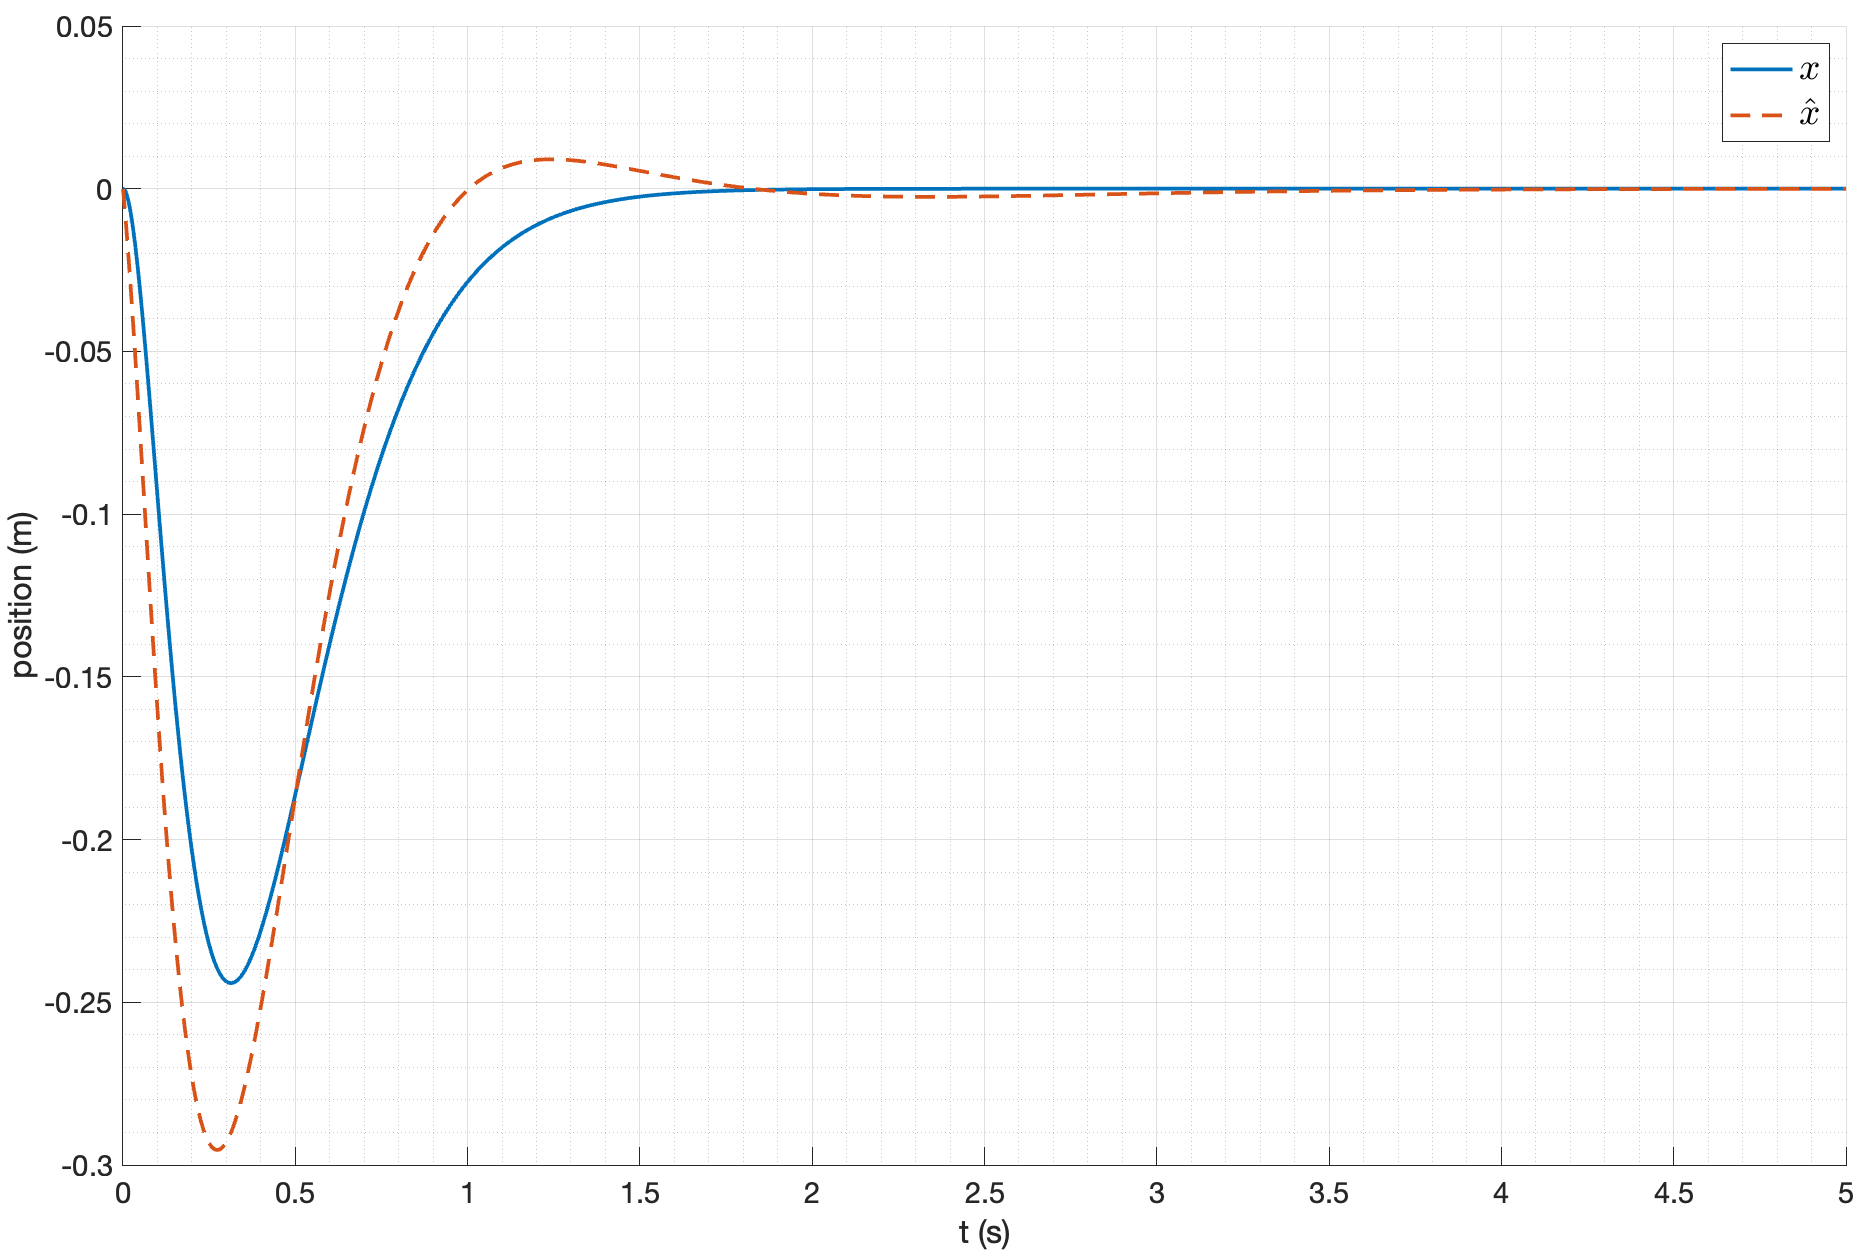
\includegraphics[width=\textwidth]{media/plots/modal_observer/observer_x_cmp_1.png}
        \caption{Оценка координаты тележки}
        \label{fig:observer_x_cmp_1}
    \end{subfigure}
    \begin{subfigure}[b]{0.45\textwidth}
        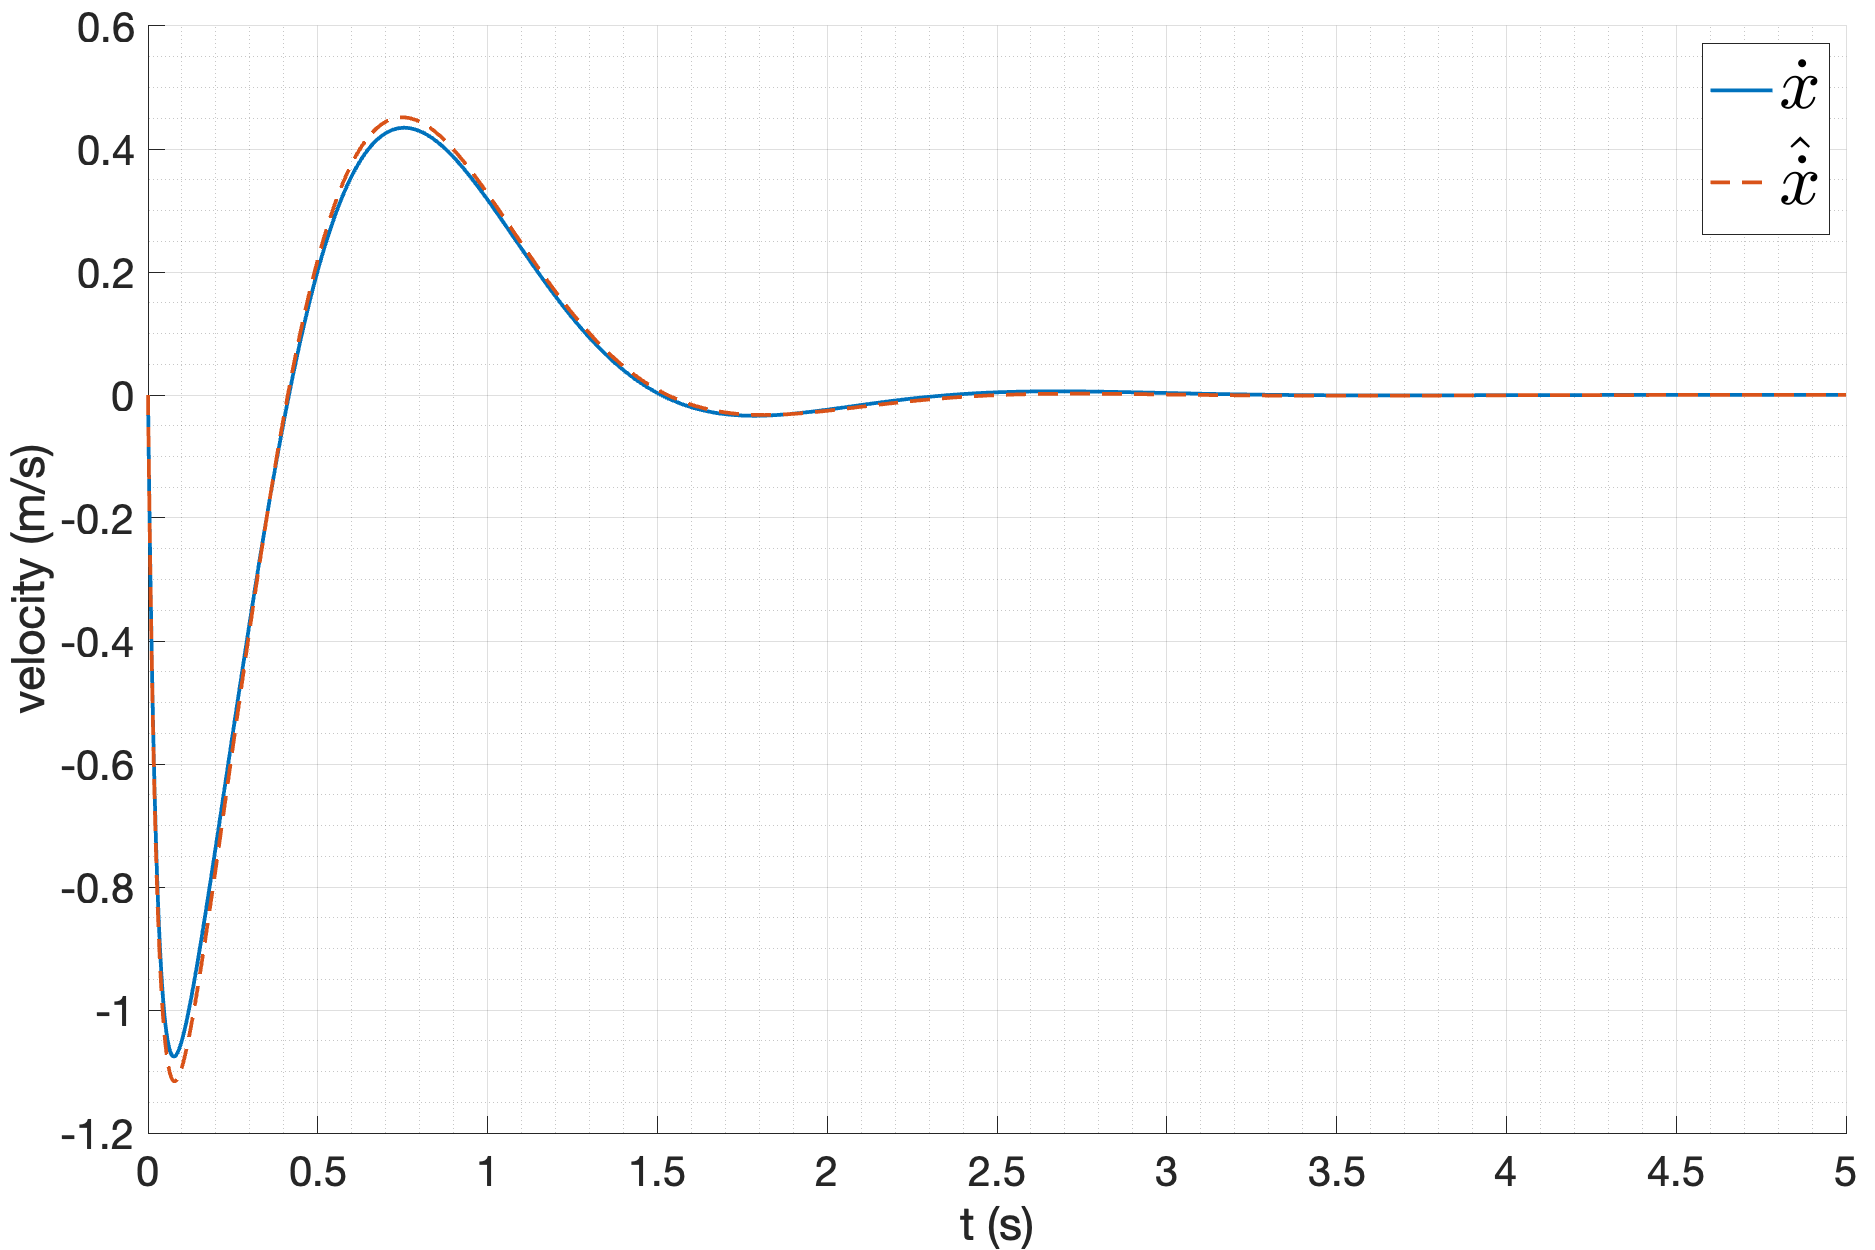
\includegraphics[width=\textwidth]{media/plots/modal_observer/observer_dotx_cmp_1.png}
        \caption{Оценка скорости тележки}
        \label{fig:observer_dotx_cmp_1}
    \end{subfigure}
    \begin{subfigure}[b]{0.45\textwidth}
        \includegraphics[width=\textwidth]{media/plots/modal_observer/observer_theta_cmp_1.png}
        \caption{Оценка угла отклонения маятника}
        \label{fig:observer_theta_cmp_1}
    \end{subfigure}
    \begin{subfigure}[b]{0.45\textwidth}
        \includegraphics[width=\textwidth]{media/plots/modal_observer/observer_dottheta_cmp_1.png}
        \caption{Оценка угловой скорости маятника}
        \label{fig:observer_dottheta_cmp_1}
    \end{subfigure}
    \caption{Сравнение оценок состояния системы с реальным состоянием}
    \label{fig:observer_x_cmp_1_sep}
\end{figure}
\FloatBarrier
Можно увидеть, что оценка состояния нелинейной системы наблюдателем полного порядка
сходится к реальному состоянию системы, при этом время переходного процесса составляет около 2 секунд.
График ошибки оценки состояния системы приведен на рисунке \ref{fig:observer_err_1}.
\begin{figure}[ht!]
    \centering
    \includegraphics[width=\textwidth]{media/plots/modal_observer/observer_err_1.png}
    \caption{Ошибка оценки состояния системы наблюдателем полного порядка}
    \label{fig:observer_err_1}
\end{figure} 

Теперь посмотрим на работу наблюдателя полного порядка с более большим по модулю спектром, например, 
$\begin{bmatrix}-10 & -10 & -10 & -10\end{bmatrix}$. Результаты моделирования приведены на
рисунке \ref{fig:observer_x_2} и \ref{fig:observer_x_cmp_2_sep}. 
\begin{figure}[ht!]
    \centering
    \includegraphics[width=\textwidth]{media/plots/modal_observer/observer_cmp_2.png}
    \caption{Результаты моделирования наблюдателя полного порядка}
    \label{fig:observer_x_2}
\end{figure}

\begin{figure}[ht!]
    \centering
    \begin{subfigure}[b]{0.45\textwidth}
        \includegraphics[width=\textwidth]{media/plots/modal_observer/observer_x_cmp_2.png}
        \caption{Оценка координаты тележки}
        \label{fig:observer_x_cmp_2}
    \end{subfigure}
    \begin{subfigure}[b]{0.45\textwidth}
        \includegraphics[width=\textwidth]{media/plots/modal_observer/observer_dotx_cmp_2.png}
        \caption{Оценка скорости тележки}
        \label{fig:observer_dotx_cmp_2}
    \end{subfigure}
    \begin{subfigure}[b]{0.45\textwidth}
        \includegraphics[width=\textwidth]{media/plots/modal_observer/observer_theta_cmp_2.png}
        \caption{Оценка угла отклонения маятника}
        \label{fig:observer_theta_cmp_2}
    \end{subfigure}
    \begin{subfigure}[b]{0.45\textwidth}
        \includegraphics[width=\textwidth]{media/plots/modal_observer/observer_dottheta_cmp_2.png}
        \caption{Оценка угловой скорости маятника}
        \label{fig:observer_dottheta_cmp_2}
    \end{subfigure}
    \caption{Сравнение оценок состояния системы с реальным состоянием при $k = -10$}
    \label{fig:observer_x_cmp_2_sep}
\end{figure}
График ошибки оценки состояния системы приведен на рисунке \ref{fig:observer_err_2}.
\begin{figure}[ht!]
    \centering
    \includegraphics[width=\textwidth]{media/plots/modal_observer/observer_err_2.png}
    \caption{Ошибка оценки состояния системы наблюдателем полного порядка}
    \label{fig:observer_err_2}
\end{figure}
\FloatBarrier
Видно, что теперь время переходного процесса составляет около 1 секунды, что меньше, чем в случае 
наблюдателя с меньшими по модулю собственными числами. 

При этом можно заметить, что начальная ошибка оценки состояния системы увеличилась, особенно сильно это заметно
для оценки угловой скорости маятника. Это может негативно сказаться на работе регулятора, замкнутого по наблюдаемому состоянию.

\subsection{Наблюдатель пониженного порядка}
Так как два значения из вектора состояния являются измеримыми, то можно использовать наблюдатель пониженного порядка, 
который будет оценивать только два оставшихся, неизмеримых состояния системы, которыми являются скорость тележки и угловая скорость маятника.

Рассмотрим наблюдатель пониженного порядка:
\begin{equation}
    \begin{array}{ll}
        \dot{\hat{z}} = \Gamma\hat{z} - Yy + QBu\\
        \hat{x} = \begin{bmatrix}
            C \\ Q
        \end{bmatrix}^{-1} \times \begin{bmatrix}
            y \\ 
            \hat{z}
        \end{bmatrix}
    \end{array}
\end{equation}
Зададим желаемый спектр наблюдателя пониженного порядка $\{-4, -5\}$.

Тогда матрица $Q$ находится из решения уравнения Сильвестра: 
\begin{equation}
   \Gamma Q - QA = YC 
\end{equation}
где $\Gamma$ -- матрица с желаемыми собственными числами. 
Решим уравнение Сильвестра с помощью пакета \texttt{cvx} в MATLAB, в результате получаем матрицу наблюдателя $Q$:
\begin{equation}
    Q = \begin{bmatrix}
    -0.25  & 0.06  & 0.02  & -0.00 \\ 
    -0.20  & 0.04  & -0.01  & 0.00 \\
    \end{bmatrix}
\end{equation}

Схема наблюдателя пониженного порядка приведена на рисунке \ref{fig:reduced_observer_scheme}.
\begin{figure}[ht!]
    \centering
    \includegraphics[width=0.7\textwidth]{media/reduced_observer_scheme.png}
    \caption{Схема наблюдателя пониженного порядка}
    \label{fig:reduced_observer_scheme}
\end{figure}

Схема включения наблюдателя в систему аналогичная схеме включения наблюдателя полного порядка, 
которая приведена на рисунке \ref{fig:observer_system}. 

Проверим работу наблюдателя пониженного порядка, сравнив его выход с реальным состоянием нелинейной системы.
Результаты моделирования приведены на рисунке \ref{fig:reduced_observer_x_1} и рисунках \ref{fig:reduced_observer_x_cmp_1_sep}.
\begin{figure}[ht!]
    \centering
    \includegraphics[width=\textwidth]{media/plots/reduced_observer/reduced_observer_cmp_1.png}
    \caption{Результаты моделирования наблюдателя пониженного порядка}
    \label{fig:reduced_observer_x_1}
\end{figure}

\begin{figure}[ht!]
    \centering
    \begin{subfigure}[b]{0.45\textwidth}
        \includegraphics[width=\textwidth]{media/plots/reduced_observer/reduced_observer_x_cmp_1.png}
        \caption{Оценка координаты тележки}
        \label{fig:reduced_observer_x_cmp_1}
    \end{subfigure}
    \begin{subfigure}[b]{0.45\textwidth}
        \includegraphics[width=\textwidth]{media/plots/reduced_observer/reduced_observer_dotx_cmp_1.png}
        \caption{Оценка скорости тележки}
        \label{fig:reduced_observer_dotx_cmp_1}
    \end{subfigure}
    \begin{subfigure}[b]{0.45\textwidth}
        \includegraphics[width=\textwidth]{media/plots/reduced_observer/reduced_observer_theta_cmp_1.png}
        \caption{Оценка угла отклонения маятника}
        \label{fig:reduced_observer_theta_cmp_1}
    \end{subfigure}
    \begin{subfigure}[b]{0.45\textwidth}
        \includegraphics[width=\textwidth]{media/plots/reduced_observer/reduced_observer_dottheta_cmp_1.png}
        \caption{Оценка угловой скорости маятника}
        \label{fig:reduced_observer_dottheta_cmp_1}
    \end{subfigure}
    \caption{Сравнение оценок состояния системы с реальным состоянием наблюдателем пониженного порядка}
    \label{fig:reduced_observer_x_cmp_1_sep}
\end{figure}
Ошибка оценки состояния системы приведена на рисунке \ref{fig:reduced_observer_err_1}.
\begin{figure}[ht!]
    \centering
    \includegraphics[width=\textwidth]{media/plots/reduced_observer/reduced_observer_err_1.png}
    \caption{Ошибка оценки состояния системы наблюдателем пониженного порядка}
    \label{fig:reduced_observer_err_1}
\end{figure}
\FloatBarrier
Видно, что оценка состояния нелинейной системы наблюдателем пониженного порядка 
не отличается от реального состояния системы для координаты тележки и угла отклонения маятника,
так как они являются напрямую измеримыми. При этом оценка скорости тележки и угловой скорости
маятника тоже сходится к реальным значениям. Время переходного процесса составляет около 1 секунды.

Рассмотрим наблюдатель пониженного порядка с желаемым спектром $\{-1, -1\}$.
Результаты моделирования приведены на рисунке \ref{fig:reduced_observer_x_2} и рисунках \ref{fig:reduced_observer_x_cmp_2_sep}.
\begin{figure}[ht!]
    \centering
    \includegraphics[width=\textwidth]{media/plots/reduced_observer/reduced_observer_cmp_2.png}
    \caption{Результаты моделирования наблюдателя пониженного порядка}
    \label{fig:reduced_observer_x_2}
\end{figure}
\begin{figure}[ht!]
    \centering
    \begin{subfigure}[b]{0.45\textwidth}
        \includegraphics[width=\textwidth]{media/plots/reduced_observer/reduced_observer_x_cmp_2.png}
        \caption{Оценка координаты тележки}
        \label{fig:reduced_observer_x_cmp_2}
    \end{subfigure}
    \begin{subfigure}[b]{0.45\textwidth}
        \includegraphics[width=\textwidth]{media/plots/reduced_observer/reduced_observer_dotx_cmp_2.png}
        \caption{Оценка скорости тележки}
        \label{fig:reduced_observer_dotx_cmp_2}
    \end{subfigure}
    \begin{subfigure}[b]{0.45\textwidth}
        \includegraphics[width=\textwidth]{media/plots/reduced_observer/reduced_observer_theta_cmp_2.png}
        \caption{Оценка угла отклонения маятника}
        \label{fig:reduced_observer_theta_cmp_2}
    \end{subfigure}
    \begin{subfigure}[b]{0.45\textwidth}
        \includegraphics[width=\textwidth]{media/plots/reduced_observer/reduced_observer_dottheta_cmp_2.png}
        \caption{Оценка угловой скорости маятника}
        \label{fig:reduced_observer_dottheta_cmp_2}
    \end{subfigure}
    \caption{Сравнение оценок состояния системы с реальным состоянием наблюдателем пониженного порядка при $k = -1$}
    \label{fig:reduced_observer_x_cmp_2_sep}
\end{figure}
График ошибки оценки состояния системы приведен на рисунке \ref{fig:reduced_observer_err_2}.
\begin{figure}[ht!]
    \centering
    \includegraphics[width=\textwidth]{media/plots/reduced_observer/reduced_observer_err_2.png}
    \caption{Ошибка оценки состояния системы наблюдателем пониженного порядка}
    \label{fig:reduced_observer_err_2}
\end{figure}
\FloatBarrier
Так же видно, что два измеримых состояния системы совпадают с реальными значениями, а два
неизмеримых состояния системы тоже сходятся к реальным значениям, но с большим временем переходного процесса,
которое составляет около 2.5 секунд.

% Проведем сравнение наблюдателей полного и пониженного порядка со спектрами $\{-4, -4, -4, -4\}$ и $\{-4, -4\}$ соответственно.
% TODO: compare observers

\subsection{Регулятор по выходу}
Рассмотрим реальный случай, когда для измерения и использования доступны только 
два из четырех состояний системы, а именно координата тележки и угол отклонения маятника.
Эти состояния могут быть измерены с помощью датчиков, установленных на системе. Для того, чтобы
стабилизировать систему будем использовать регулятор, основанный на оценке состояния системы 
наблюдателем пониженного порядка. 

Порядок синтеза модального регулятора и наблюдателя пониженного порядка приведен выше. 
Схема моделирования приведена на рисунке \ref{fig:modal_controller_obderver}.
Выход подсистемы, соответствующий вектору состояния не используется, что 
имитирует реальный случай, когда для управления доступны только два состояния системы. 

\begin{figure}[ht!]
    \centering
    \includegraphics[width=0.7\textwidth]{media/model_controller_observer.png}
    \caption{Схема моделирования регулятора по выходу}
    \label{fig:modal_controller_obderver}
\end{figure} 

Подберем спектры регулятора и наблюдателя пониженного порядка таким образом, чтобы 
достичь наилучшего качества переходного процесса. Наилучшего результата удалось достичь при
спектрах $\{-9, -9, -9, -9\}$ и $\{-5, -5\}$ для регулятора и наблюдателя соответственно. 
Выход системы, замкнутой регулятором по выходу, приведен на рисунке \ref{fig:modal_controller_obderver_out}.
\begin{figure}[ht!]
    \centering
    \includegraphics[width=\textwidth]{media/plots/observer_controller/observer_controller_out.png}
    \caption{Результаты моделирования регулятора по выходу}
    \label{fig:modal_controller_obderver_out}
\end{figure}

Система стабилизируется, при этом время переходного процесса составляет около 1.8 секунд. 
График управляющего воздействия приведен на рисунке \ref{fig:modal_controller_obderver_u}.
\begin{figure}[ht!]
    \centering
    \includegraphics[width=\textwidth]{media/plots/observer_controller/observer_controller_u.png}
    \caption{Управляющее воздействие регулятора по выходу}
    \label{fig:modal_controller_obderver_u}
\end{figure}
Максимальное по модулю управляющее воздействие составляет около 15000 Н. Величина, довольно большая, 
но может быть объяснена тем, что масса тележки составляет 255кг. 

\FloatBarrier
\subsection{Выводы} 
В данной главе были рассмотрены модальные регуляторы и наблюдатели. Были рассмотрены влияния собственных 
чисел замкнутой системы на динамику системы, а также влияние собственных чисел на работу наблюдателя. 
Исследовано влияние начальных условий на работу системы. Ожидаемым результатом оказалось то, что 
при увеличении модуля собственных чисел замкнутой системы, время переходного процесса уменьшается, 
при этом увеличивается перерегулирование и максимальное по модулю управляющее воздействие. 
Влияние начальных условий на работу системы оказалось тоже весьма ожидаемым. При увеличении 
начального отклонения маятника увеличивается расхождение между линеаризованной моделью и реальной системой, 
что приводит к ошибкам в управлении. Начиная с некоторого значения начального отклонения, 
на практике оказавшегося равным 1.2 радиан, система не может быть стабилизирована. 
\FloatBarrier
\section{Регуляторы с заданной степенью устойчивости}
Рассмотрим немодальные методы синтеза регуляторов, которые позволяют задать степень устойчивости системы
в целом, а не выбирать каждое собственное число самостоятельно. Для этого будем использовать 
решение матричного неравенства Ляпунова: 
\begin{equation}
    PA^T + AP + 2\alpha P + Y^T B^T + BY \preceq 0, ~~~ K = Y P^{-1}, ~~~ P \succ 0
\end{equation}
Для решения данного неравенства воспользуемся пакетом \texttt{cvx} в MATLAB. 

Зададимся значением степени устойчивости $\alpha = 3$ и синтезируем регулятор на основе матриц линейной системы. 
В результате получаем матрицу регулятора $K$: 
\begin{equation}
    K = \begin{bmatrix}
    18189.83  & 11279.39  & -35086.93  & -8004.31 \\ 
    \end{bmatrix}
\end{equation}
Проверим правильность полученного решения, найдя собственные числа замкнутой системы:
\begin{equation}
    \sigma(A + BK) = \begin{bmatrix}
    -4.52 + 8.36j \\ 
    -4.52 - 8.36j \\ 
    -4.34 \\ 
    -3.46 \\ 
    \end{bmatrix}
\end{equation}
По собственным числам делаем вывод, что степень устойчивости системы равна $3.46$, 
что несколько больше, чем заданное значение $\alpha = 3$. Делаем вывод, что 
получен корректный регулятор. 

\subsection{Исследование устойчивости при различных начальных условиях}
Проверим работу данного регулятора при различных начальных условиях. 
В качестве начальных условий возьмем различные начальные углы отклонения маятника $\theta_0 \in \begin{bmatrix}0.3, 0.4, 0.6, 0.8\end{bmatrix}$. Результаты 
моделирования приведены на рисунке \ref{fig:nonmodal_control_initials}. 
При большем начальном отклонении от положения равновесия моделирование провести не удалось. Это может быть связано с тем, 
что система становится неустойчивой при больших отклонениях, и численное решение такой системы становится слишком долгим. 
\begin{figure}[ht!]
    \centering
    \begin{subfigure}[b]{0.45\textwidth}
        \includegraphics[width=\textwidth]{media/plots/nonmodal_control/out_1.png}
        \caption{$\theta_0 = 0.3$}
    \end{subfigure}
    \begin{subfigure}[b]{0.45\textwidth}
        \includegraphics[width=\textwidth]{media/plots/nonmodal_control/out_2.png}
        \caption{$\theta_0 = 0.4$}
    \end{subfigure}
    \begin{subfigure}[b]{0.45\textwidth}
        \includegraphics[width=\textwidth]{media/plots/nonmodal_control/out_3.png}
        \caption{$\theta_0 = 0.6$}
    \end{subfigure}
    \begin{subfigure}[b]{0.45\textwidth}
        \includegraphics[width=\textwidth]{media/plots/nonmodal_control/out_4.png}
        \caption{$\theta_0 = 0.8$}
    \end{subfigure}
    \caption{Модальное управление нелинейной модели системы}
    \label{fig:nonmodal_control_initials}
\end{figure}

На графиках видно, что система стабилизируется к положению равновесия при различных начальных условиях. При этом, 
чем больше начальное отклонение, тем больше требуется времени для стабилизации системы и тем больше перерегулирование. 

\subsection{Исследование переходного процесса} 
Будем рассматривать переходный процесс и управляющее воздействие при различных степенях устойчивости $\alpha$ регулятора. 
В качестве начальных условий возьмем $\theta_0 = 0.3$. В качестве степеней устойчивости будем использовать 
значения $\alpha \in \begin{bmatrix} 1, 3, 6\end{bmatrix}$. Для каждого значения $\alpha$ будем 
синтезировать регулятор и исследовать его влияние на переходный процесс. 

Полученные регуляторы: 
\begin{enumerate}
    \item $\alpha = 1$: $K = \begin{bmatrix} 2180.49  & 2549.34  & -11475.12  & -2606.25 \\ \end{bmatrix}$, $\sigma(A + BK) = \begin{bmatrix} -2.12 + 5.02j \\ -2.12 - 5.02j \\ -4.35 \\ -1.26 \\  \end{bmatrix}$
    \item \item $\alpha = 3$: $K = \begin{bmatrix} 18189.83  & 11279.39  & -35086.93  & -8004.31 \\ \end{bmatrix}$, $\sigma(A + BK) = \begin{bmatrix} -4.52 + 8.36j \\ -4.52 - 8.36j \\ -4.34 \\ -3.46 \\  \end{bmatrix}$
    \item $\alpha = 6$: $K = \begin{bmatrix} 230529.7  & 76168.3  & -208685.7  & -43384.3 \\ \end{bmatrix}$, $\sigma(A + BK) = \begin{bmatrix} -9.84 + 16.2j \\ -9.84 - 16.2j \\ -6.55 + 2.1j \\ -6.55 - 2.1j \\ \end{bmatrix}$
\end{enumerate}
Все регуляторы синтезировались корректно, устойчивость каждой системы соответствует заданной степени устойчивости $\alpha$. 

Проведем моделирование переходного процесса для каждого из полученных регуляторов. 

Результаты моделирования приведены на рисунках \ref{fig:nonmodal_control_alpha_1} - \ref{fig:nonmodal_control_alpha_3_u}.
Сравнительные графики переходных процессов приведены на рисунке \ref{fig:nonmodal_control_cmp_x} и \ref{fig:nonmodal_control_cmp_ang}.

\begin{figure}[ht!]
    \centering
    \includegraphics[width=\textwidth]{media/plots/nonmodal_controllers/out_1.png}
    \caption{Переходный процесс при $\alpha = 1$}
    \label{fig:nonmodal_control_alpha_1}
\end{figure}
\begin{figure}[ht!]
    \centering
    \includegraphics[width=\textwidth]{media/plots/nonmodal_controllers/u_1.png}
    \caption{Управляющее воздействие при $\alpha = 1$}
    \label{fig:nonmodal_control_alpha_1_u}
\end{figure}
\begin{figure}[ht!]
    \centering
    \includegraphics[width=\textwidth]{media/plots/nonmodal_controllers/out_2.png}
    \caption{Переходный процесс при $\alpha = 3$}
    \label{fig:nonmodal_control_alpha_2}
\end{figure}
\begin{figure}[ht!]
    \centering
    \includegraphics[width=\textwidth]{media/plots/nonmodal_controllers/u_2.png}
    \caption{Управляющее воздействие при $\alpha = 3$}
    \label{fig:nonmodal_control_alpha_2_u}
\end{figure}
\begin{figure}[ht!]
    \centering
    \includegraphics[width=\textwidth]{media/plots/nonmodal_controllers/out_3.png}
    \caption{Переходный процесс при $\alpha = 6$}
    \label{fig:nonmodal_control_alpha_3}
\end{figure}
\begin{figure}[ht!]
    \centering
    \includegraphics[width=\textwidth]{media/plots/nonmodal_controllers/u_3.png}
    \caption{Управляющее воздействие при $\alpha = 6$}
    \label{fig:nonmodal_control_alpha_3_u}
\end{figure}

\begin{figure}[ht!]
    \centering
    \includegraphics[width=\textwidth]{media/plots/nonmodal_controllers/x_cmp.png}
    \caption{Сравнение переходных процессов по смещению тележки}
    \label{fig:nonmodal_control_cmp_x}
\end{figure}
\begin{figure}[ht!]
    \centering
    \includegraphics[width=\textwidth]{media/plots/nonmodal_controllers/ang_cmp.png}
    \caption{Сравнение переходных процессов по углу отклонения маятника}
    \label{fig:nonmodal_control_cmp_ang}
\end{figure}

\FloatBarrier
Как и ожидалось, при увеличении степени устойчивости $\alpha$ уменьшается время переходного процесса, но при этом 
увеличивается перерегулирование. При $\alpha = 1$ система стабилизируется приблизительно за $3$ секунды, а 
при $\alpha = 6$ -- за $1$ секунду. При этом, при $\alpha = 1$ максимальное отклонение от положения равновесия составляет 
$0.4$ радиан, а при $\alpha = 6$ -- $0.4$ радиан. 

Управляющее воздействие при увеличении степени устойчивости $\alpha$ также увеличивается. При $\alpha = 1$ максимальное
управляющее воздействие составляет $1500$ Н, а при $\alpha = 6$ -- $19000$. 

\subsection{Исследование регулятора с ограничением на управление} 
Рассмотрим такую же задачу нахождения регулятора, обеспечивающего заданную степень устойчивости 
системы, но теперь добавим условие минимальности управления. Неравенства в данном случае 
будут следующими:
\begin{equation}
    \begin{array}{cc}
        PA^T + AP + 2\alpha P + Y^T B^T + BY \preceq 0, ~~~ K = Y P^{-1}, ~~~ P \succ 0 \\ 
        \begin{bmatrix}
            P & x(0) \\
            x(0)^T & 1
        \end{bmatrix} \succ 0, ~~~ \begin{bmatrix}
            P & Y^T \\
            Y & \mu^2I
        \end{bmatrix} \succ 0
    \end{array}
\end{equation} 
где $\mu$ -- ограничение на управление $\mu \ge \|u(t)\|_2$.

Для синтеза регулятора зададимся начальными условиями $x_0 = \begin{bmatrix} 0 & 0 & 0.05 & 0.0 \end{bmatrix}^T$. 

Для значения $\alpha = 0.1$ получаем регулятор:
\begin{equation}
    K = \begin{bmatrix}
    3.85  & 40.27  & -2813.02  & -548.59 \\ 
    \end{bmatrix}
\end{equation}
С значением $\mu = 28.89$ и собственными числами замкнутой системы:
\begin{equation}
     \sigma(A + BK) = \begin{bmatrix}
        -5.13 \\ 
        -0.10 + 0.86j \\ 
        -0.10 - 0.86j \\ 
        -0.10 \\ 
    \end{bmatrix}
\end{equation}  
Система устойчива, степень устойчивости равна $0.1$, что в точности соответствует заданному значению $\alpha = 0.1$,
в отличие от регулятора, синтезированного без условия минимизации управляющего воздействия, где степень устойчивости 
получалась больше заданной.

Проведем моделирование данной системы при начальном угле отклонения маятника $\theta_0 = \in \begin{bmatrix} 0.05, 0.3, 0.8\end{bmatrix}$. 
Результаты моделирования приведены на рисунках \ref{fig:nonmodal_control_alpha_1_1} - \ref{fig:nonmodal_control_alpha_1_3}.
\begin{figure}[ht!]
    \centering
    \includegraphics[width=\textwidth]{media/plots/nonmodal_controlers_min/out_1.png}
    \caption{Переходный процесс при $\alpha = 0.1$ и $\theta_0 = 0.05$}
    \label{fig:nonmodal_control_alpha_1_1}
\end{figure}
\begin{figure}[ht!]
    \centering
    \includegraphics[width=\textwidth]{media/plots/nonmodal_controlers_min/out_2.png}
    \caption{Переходный процесс при $\alpha = 0.1$ и $\theta_0 = 0.3$}
    \label{fig:nonmodal_control_alpha_1_2}
\end{figure}
\begin{figure}[ht!]
    \centering
    \includegraphics[width=\textwidth]{media/plots/nonmodal_controlers_min/out_3.png}
    \caption{Переходный процесс при $\alpha = 0.1$ и $\theta_0 = 0.8$}
    \label{fig:nonmodal_control_alpha_1_3}
\end{figure}
\FloatBarrier
Видно, что при небольших начальных условиях система стабилизируется к положению равновесия,
при этом при больших начальных условиях время стабилизации увеличивается, система начинает
больше колебаться. 
Синтез такого регулятора проводится в условиях известных начальных условий, 
и отклонение от них может привести к некорректной работе регулятора. 

\subsection{Исследование переходного процесса}
Рассмотрим поведение системы с регуляторами с различными заданными степенями устойчивости 
$\alpha \in \begin{bmatrix}0.05, 0.5, 1.0\end{bmatrix}$ и начальным углом отклонения маятника 
$\theta_0 = 0.1$. 

При $\alpha = 0.05$ получены следующие результаты: 
\begin{equation}
    K = \begin{bmatrix} 0.95  & 19.50  & -2715.72  & -613.74 \end{bmatrix}, \sigma(A + BK) = \begin{bmatrix} -4.43 \\ -0.05 + 0.56j \\ -0.05 - 0.56j \\ -0.05  \end{bmatrix}
\end{equation}
Желаемая степень устойчивости достигнута. Проведем моделирование системы. Результаты 
представлены на рисунке \ref{fig:nonmodal_control_alpha_2_1}.

\begin{figure}[ht!]
    \centering
    \includegraphics[width=\textwidth]{media/plots/nonmodal_controlers_min/out_4.png}
    \caption{Переходный процесс при $\alpha = 0.05$}
    \label{fig:nonmodal_control_alpha_2_1}
\end{figure}

\FloatBarrier
При $\alpha = 0.5$ получены следующие результаты: 
\begin{equation}
    K = \begin{bmatrix} 111.01  & 276.86  & -4075.74  & -923.80  \\ \end{bmatrix}, \sigma(A + BK) = \begin{bmatrix} -4.43 \\ -0.50 + 1.87j \\ -0.50 - 1.87j \\ -0.50 \\ \end{bmatrix}
\end{equation}
Желаемая степень устойчивости достигнута. Проведем моделирование системы. Результаты 
представлены на рисунках \ref{fig:nonmodal_control_alpha_2_1} - \ref{fig:nonmodal_control_alpha_2_3}

\begin{figure}[ht!]
    \centering
    \includegraphics[width=\textwidth]{media/plots/nonmodal_controlers_min/out_5.png}
    \caption{Переходный процесс при $\alpha = 0.5$}
    \label{fig:nonmodal_control_alpha_2_2}
\end{figure} 

\FloatBarrier
При $\alpha = 1.0$ получены следующие результаты: 
\begin{equation}
    K = \begin{bmatrix} -14.94  & -22.76  & 1.78  & 0.64  \end{bmatrix}, \sigma(A + BK) = \begin{bmatrix} -4.43 \\ -0.04 + 0.23j \\ -0.04 - 0.23j \\ 4.43 \\ \end{bmatrix}
\end{equation}
Решение данной системы не было найдено, собственные числа системы не соответствуют заданной степени устойчивости.
Кроме того, с полученным регулятором система не является устойчивой, что связано с наличием 
собственного числа с положительной действительной частью.

\begin{figure}[ht!]
    \centering
    \includegraphics[width=\textwidth]{media/plots/nonmodal_controlers_min/out_6.png}
    \caption{Переходный процесс при $\alpha = 1.0$}
    \label{fig:nonmodal_control_alpha_2_3}
\end{figure} 
\FloatBarrier 

Видно, что при увеличении степени устойчивости система сходится быстрее, при этом 
максимальное отклонение от положения равновесия тоже уменьшается. 
Получить регулятор с $\alpha = 1.0$ не удалось. 

\subsection{Синтез наблюдателя}
Использую линейные матричные неравенства Ляпунова проведем синтез 
наблюдателя полной размерности $\hat{x} = A\hat{x} + Bu + L(\hat{y} - y)$: 
\begin{equation}
    A^TQ + QA + 2\alpha Q + C^T Y^T + YC \preceq 0, ~~~ L = Q^{-1}Y, ~~~ Q \succ 0
\end{equation}
Решая данное неравенство для $\alpha = 3$ получаем матрицу наблюдателя: 
\begin{equation}
   L_1 = \begin{bmatrix}
    -10.33  & 0.06 \\ 
    -44.18  & -0.40 \\ 
    -0.15  & -13.19 \\ 
    -0.85  & -77.03 \\ 
    \end{bmatrix}
\end{equation}
Проверим устойчивость наблюдателя, найдя собственные числа системы $(A + L_1C)$: 
\begin{equation}
    \sigma(A - L_1C) = \begin{bmatrix}
        -5.17 + 4.18j \\ 
        -5.17 - 4.18j \\ 
        -6.59 + 3.74j \\ 
        -6.59 - 3.74j \\ 
    \end{bmatrix}
\end{equation}
По собственным числам видно, что наблюдатель устойчив, степень устойчивости равна $5.17$, что больше, чем заданное значение $\alpha = 3$. 

Для дальнейшего исследования проведем синтез еще одного наблюдателя $L_2$ со степенью устойчивости $\alpha = 10$.
Решая неравенство Ляпунова для $\alpha = 10$ получаем матрицу наблюдателя:
\begin{equation}
    L_2 = \begin{bmatrix}
    -31.54  & -0.07 \\ 
    -422.53  & -1.54 \\ 
    -0.17  & -33.90 \\ 
    -2.48  & -401.44 \\
    \end{bmatrix}
\end{equation}
Проверим устойчивость наблюдателя, найдя собственные числа системы $(A + L_2C)$:
\begin{equation}
    \sigma(A - L_2C) = \begin{bmatrix}
    -15.77 + 13.18j \\ 
    -15.77 - 13.18j \\ 
    -16.95 + 9.72j \\ 
    -16.95 - 9.72j \\
    \end{bmatrix}
\end{equation}
Желаемая степень устойчивости так же достигнута. Можно делать вывод о корректности синтеза наблюдателя. 

\subsection{Управление по выходу}
Рассмотрим управление системой, когда к измерению доступны только выходные переменные. Для этого будем использовать
наблюдатель и регулятор, полученные ранее (через матричные неравенства Ляпунова).

Возьмем два регулятора с различными степенями устойчивости $\alpha = 3$ и $\alpha = 10$: 
\begin{equation}
    \begin{array}{cc}
        K_1 = \begin{bmatrix}
        18189.83  & 11279.39  & -35086.93  & -8004.31 \\ 
        \end{bmatrix}  \\ 
        K_2 = \begin{bmatrix}
        1166417.18  & 245556.29  & -784739.34  & -132290.09 \\ 
        \end{bmatrix}
    \end{array}
\end{equation}
И два наблюдателя с различными степенями устойчивости $\alpha = 3$ и $\alpha = 10$:
\begin{equation}
    \begin{array}{cc}
        L_1 = \begin{bmatrix}
        -10.33  & 0.06 \\ 
        -44.18  & -0.40 \\ 
        -0.15  & -13.19 \\ 
        -0.85  & -77.03 \\ 
        \end{bmatrix} \\[3em]
        L_2 = \begin{bmatrix}
        -31.54  & -0.07 \\ 
        -422.53  & -1.54 \\ 
        -0.17  & -33.90 \\ 
        -2.48  & -401.44 \\ 
        \end{bmatrix}
    \end{array}
\end{equation}

Проведем моделирование систем с парами регуляторов и наблюдателей $(K_1, L_1)$, $(K_2, L_1)$ и $(K_2, L_2)$. Схема моделирования 
представлена на рисунке \ref{fig:KL_scheme}. 
\begin{figure}[ht!]
    \centering
    \includegraphics[width=0.8\textwidth]{media/KL_scheme.png}
    \caption{Схема моделирования системы с регулятором и наблюдателем}
    \label{fig:KL_scheme}   
\end{figure}
В качестве начальных условий возьмем $e_0 = \begin{bmatrix} 0 & 0 & 0 & 0 \end{bmatrix}^T$ для наблюдателя
и $x_0 = \begin{bmatrix} 0 & 0 & 0.2 & 0 \end{bmatrix}^T$ для системы. 

Результаты моделирования для пары $(K_1, L_1)$ приведены на рисунках \ref{fig:KL_1_out} - \ref{fig:KL_1_err}. 
\begin{figure}[ht!]
    \centering
    \includegraphics[width=\textwidth]{media/plots/nonmodal_observer_controller/kl_1.png}
    \caption{Переходный процесс при $(K_1, L_1)$}
    \label{fig:KL_1_out}
\end{figure}
\begin{figure}[ht!]
    \centering
    \includegraphics[width=\textwidth]{media/plots/nonmodal_observer_controller/kl_err_1.png}
    \caption{Ошибка наблюдения при $(K_1, L_1)$}
    \label{fig:KL_1_err}
\end{figure}
\FloatBarrier

Результаты моделирования для пары $(K_2, L_1)$ приведены на рисунках \ref{fig:KL_2_out} - \ref{fig:KL_2_err}.
\begin{figure}[ht!]
    \centering
    \includegraphics[width=\textwidth]{media/plots/nonmodal_observer_controller/kl_2.png}
    \caption{Переходный процесс при $(K_2, L_1)$}
    \label{fig:KL_2_out}
\end{figure}
\begin{figure}[ht!]
    \centering
    \includegraphics[width=\textwidth]{media/plots/nonmodal_observer_controller/kl_err_2.png}
    \caption{Ошибка наблюдения при $(K_2, L_1)$}
    \label{fig:KL_2_err}
\end{figure}
\FloatBarrier

Результаты моделирования для пары $(K_1, L_2)$ приведены на рисунках \ref{fig:KL_3_out} - \ref{fig:KL_3_err}.
\begin{figure}[ht!]
    \centering
    \includegraphics[width=\textwidth]{media/plots/nonmodal_observer_controller/kl_3.png}
    \caption{Переходный процесс при $(K_1, L_2)$}
    \label{fig:KL_3_out}
\end{figure}
\begin{figure}[ht!]
    \centering
    \includegraphics[width=\textwidth]{media/plots/nonmodal_observer_controller/kl_err_3.png}
    \caption{Ошибка наблюдения при $(K_1, L_2)$}
    \label{fig:KL_3_err}
\end{figure}

\FloatBarrier
По результатам исследования можно сделать вывод, что регулятор и наблюдатель вместе влияют на переходный процесс.
В первой паре, с \textit{слабым} регулятором и \textit{слабым} наблюдателем, система стабилизируется к положению равновесия
приблизительно за $3$ секунды, при этом ошибка наблюдения (для измерения угла отклонения маятника) приходит к нулю
за то же время. Во второй паре, с \textit{сильным} регулятором и \textit{слабым} наблюдателем, система стабилизируется
к положению равновесия приблизительно за $2.5$ секунды, при этом ошибка наблюдения также приходит к нулю за это же время, 
но ошибка наблюдения в начальный момент времени больше, чем в первой паре. В дальнейшем ошибка наблюдения становится 
примерно такой же, как и в первой паре. В третьей паре, с \textit{слабым} регулятором и \textit{сильным} наблюдателем,
система стабилизируется к положению равновесия приблизительно за $2.5$ секунды, при этом ошибка наблюдения
приходит к нулю за $1.5$ секунды, что меньше, чем в обоих предыдущих парах. 

Таким образом, можно сделать вывод, что при увеличении степени устойчивости как регулятора, так и наблюдателя,
система стабилизируется быстрее.

\subsection{Выводы}
В данной главе были рассмотрены немодальные методы синтеза регуляторов, которые позволяют задать степень устойчивости системы в целом.
Были синтезированы регуляторы с заданной степенью устойчивости, проведено исследование переходного процесса и управляющего воздействия при различных начальных условиях и степенях устойчивости.
Также были синтезированы регуляторы с ограничением на управление, позволяющие минимизировать управляющее воздействие.
Было рассмотрено управление системой по выходу, когда неизмеряемые состояния системы восстанавливаются с помощью наблюдателя. 
Это может быть полезно в реальных системах, где не все состояния могут быть измерены напрямую. 

\FloatBarrier
\section{Слежение и компенсация}
\subsection{Задание сигнала}
Зададим сигнал $f$, состоящий из пяти гармоник следующим образом:
\begin{equation}
    f(t) = \sum_{i=1}^{5} A_i \cos(\omega_i t + \phi_i)
\end{equation}
Запишем систему, описывающую генератор внешнего возмущения: 
\begin{equation}
    \begin{cases}
        \dot{\omega}_f = \Gamma_f \omega_f \\
        f = Y_f \omega_f
    \end{cases}
\end{equation}
где $\Gamma_f$ -- матрица гармоник, $Y_f$ -- матрица весов. 

Таким образом, для задания внешнего возмущения $f(t)$ необходимо задать матрицы 
$\Gamma_f$, $Y_f$ и начальное значение $w_f(0)$. 

Пусть матрица $\Gamma_f$ имеет вид:
\begin{equation}
    \Gamma_f = \begin{bmatrix}
        0 & -1 & 0 & 0 & 0 & 0 & 0 & 0 & 0 & 0 \\
        1 & 0 & 0 & 0 & 0 & 0 & 0 & 0 & 0 & 0 \\
        0 & 0 & 0 & -2 & 0 & 0 & 0 & 0 & 0 & 0 \\
        0 & 0 & 2 & 0 & 0 & 0 & 0 & 0 & 0 & 0 \\
        0 & 0 & 0 & 0 & 0 & -3 & 0 & 0 & 0 & 0 \\
        0 & 0 & 0 & 0 & 3 & 0 & 0 & 0 & 0 & 0 \\
        0 & 0 & 0 & 0 & 0 & 0 & 0 & -4 & 0 & 0 \\
        0 & 0 & 0 & 0 & 0 & 0 & 4 & 0 & 0 & 0 \\
        0 & 0 & 0 & 0 & 0 & 0 & 0 & 0 & 0 & -5 \\
        0 & 0 & 0 & 0 & 0 & 0 & 0 & 0 & 5 & 0 \\
    \end{bmatrix}
\end{equation}

Матрица весов $Y_f$ может быть задана как:
\begin{equation}
    Y_f = \begin{bmatrix}
        0.3 & -0.5 & 0.2 & -1.0 & 0.9 & 0.4 & 0.6 & 0.8 & -0.7 & 0.1 \\
    \end{bmatrix}
\end{equation}
и начальное значение $w_f(0)$:
\begin{equation}
    w_f(0) = \begin{bmatrix}
        1.0 & 0 & 0 & 0 & 0.3 & 0 & 0 & 0 & 0.5 & 0 \\
    \end{bmatrix}^T
\end{equation}

Промоделируем полученную систему. Результат моделирования представлен на рисунке \ref{fig:signal_generation}.
\begin{figure}[ht!]
    \centering
    \includegraphics[width=\textwidth]{media/plots/compensation/force.png}
    \caption{График сгенерированного сигнала $f(t)$}
    \label{fig:signal_generation}
\end{figure}

\subsection{Компенсирующий регулятор}
Рассмотрим регулятор, способный компенсировать влияние внешнего возмущения $f(t)$ на систему. Пусть регулятор имеет вид:
\begin{equation}
    u(t) = Kx + K_f w_f 
\end{equation}
где $K$ -- feedback компонента, $K_f$ -- feedforward компонента. 

Для синтеза feedback компонентны будем использовать уже рассмотренный ранее метод LQR.
Для заданной степени устойчивости $\alpha = 2$ получает матрицу регулятора $K$:
\begin{eqnarray}
    K = \begin{bmatrix}
        8804.48  & 6658.07  & -23113.34  & -5271.36 \\ 
    \end{bmatrix}
\end{eqnarray}
С собственными числами замкнутой системы:
\begin{equation}
    \sigma(A + BK) = \begin{bmatrix}
        -3.63 + 6.93j \\ 
        -3.63 - 6.93j \\ 
        -4.38 \\ 
        -2.44 \\ 
    \end{bmatrix}
\end{equation}

Для синтеза feedforward компоненты $K_f$ рассмотрим систему:
\begin{equation}
    \begin{cases}
        P\Gamma_f - AP = BY + DY_f \\ 
        C_z P = 0 \\ 
        K_f = Y - K P \\ 
    \end{cases}
\end{equation}
где $C_z$ -- матрица виртуального выхода системы, обеспечивающий заданное условие 
сходимости угла отклонения маятника к нулю
\begin{equation}
    \lim_{t\to\infty} ||\theta|| = 0
\end{equation}
Условием существования такого регулятора является принадлежность собственных чисел 
внешнего возмущения правой комплексной полуплоскости и принадлежность корней 
системы, замкнутой регулятором, левой комплексной полуплоскости. Оба эти условия выполняются. 
Решим систему с помощью пакета \texttt{cvx} в MATLAB, в результате получаем:
\begin{equation}
    K_f = \begin{bmatrix}
190.03  & 2039.24  & 885.49  & 977.38  & -626.11  & 468.55  & -568.20  & 108.56  & 92.98  & -310.25 \\
    \end{bmatrix}
\end{equation}

\subsection{Моделирование}
Проведем моделирование линейной системы с полученным регулятором при наличии внешнего возмущения $f(t)$. 
Результат моделирования представлен на рисунке \ref{fig:compensation_lin}.
\begin{figure}[ht!]
    \centering
    \includegraphics[width=\textwidth]{media/plots/compensation/linear_out_1.png}
    \caption{График выхода линейной системы с компенсирующим регулятором}
    \label{fig:compensation_lin}
\end{figure}
Видно, что как и было необходимо, угловое отклонение маятника стремится к нулю, при этом 
положение тележки не сходится к нулю. 

График изменение вектора состояние линейной системы с компенсирующим регулятором представлен на рисунке \ref{fig:compensation_lin_state}.
\begin{figure}[ht!]
    \centering
    \includegraphics[width=0.8\textwidth]{media/plots/compensation/linear_state_1.png}
    \caption{График изменения вектора состояния линейной системы с компенсирующим регулятором}
    \label{fig:compensation_lin_state}
\end{figure}

Проведем моделирование нелинейной системы с полученным регулятором при наличии внешнего возмущения $f(t)$.
Результат моделирования представлен на рисунке \ref{fig:compensation_nlin}.
\begin{figure}[ht!]
    \centering
    \includegraphics[width=0.8\textwidth]{media/plots/compensation/out_1.png}
    \caption{График выхода нелинейной системы с компенсирующим регулятором}
    \label{fig:compensation_nlin}
\end{figure}
Как и в случае линейной системы, угловое отклонение маятника стремится к нулю, при этом 
положение тележки не сходится к нулю. 
График изменение вектора состояние нелинейной системы с компенсирующим регулятором представлен на рисунке \ref{fig:compensation_nlin_state}.
\begin{figure}[ht!]
    \centering
    \includegraphics[width=0.8\textwidth]{media/plots/compensation/state_1.png}
    \caption{График изменения вектора состояния нелинейной системы с компенсирующим регулятором}
    \label{fig:compensation_nlin_state}
\end{figure}
График управляющего воздействия нелинейной системы с компенсирующим регулятором представлен на рисунке \ref{fig:compensation_nlin_control}.
\begin{figure}[ht!]
    \centering
    \includegraphics[width=0.8\textwidth]{media/plots/compensation/u_1.png}
    \caption{График управляющего воздействия нелинейной системы с компенсирующим регулятором}
    \label{fig:compensation_nlin_control}
\end{figure}
\FloatBarrier
Таким образом, полученный регулятор успешно справляется с компенсацией внешнего возмущения $f(t)$,
условие сходимости угла отклонения маятника к нулю выполняется, при этом положение тележки не стремится к нулю.
Полученный регулятор работает корректно как в линейной, так и в нелинейной системе. 

\subsection{Слежение за внешним возмущением}
Возьмем тот же сигнал $g(t) = f(t)$, что и в предыдущем пункте, и рассмотрим систему слежения за этим сигналом:  
\begin{equation}
    \lim_{t\to\infty} ||\theta(t) - g(t)|| = 0
\end{equation}
регулятор будет иметь вид:
\begin{equation}
    u(t) = Kx + K_g w_f
\end{equation}
В качестве feedback компоненты $K$ будем использовать уже рассмотренный ранее регулятор LQR: 
\begin{eqnarray}
    K = \begin{bmatrix}
        8804.48  & 6658.07  & -23113.34  & -5271.36 \\ 
    \end{bmatrix}
\end{eqnarray}
Для синтеза feedforward компоненты $K_g$ рассмотрим систему:
\begin{equation}
    \begin{cases}
        P\Gamma_f - AP = BY \\
        C_z P - Y_g = 0 \\
        K_g = Y - K P \\
    \end{cases}
\end{equation}
Решив систему с помощью пакета \texttt{cvx} в MATLAB, получаем:
\begin{equation}
    K_g = \begin{bmatrix}
        -10582  & -54283  & -27722  & -11896  & 1774  & -16672  & 2018  & -12144  & 6860  & 1718 \\ 
    \end{bmatrix}
\end{equation}
\subsection{Моделирование}
Проведем моделирование линейной системы с полученным регулятором для слежения за задающим сигналом $g(t)$.
Результат моделирования представлен на рисунке \ref{fig:tracking_lin}.
\begin{figure}[ht!]
    \centering
    \includegraphics[width=0.8\textwidth]{media/plots/follow/linear_out_1.png}
    \caption{График выхода линейной системы с регулятором слежения}
    \label{fig:tracking_lin}
\end{figure}
Построим график угла отклонения маятника и задающего сигнала $g(t)$ на одном графике для наглядности.
Результат представлен на рисунке \ref{fig:tracking_lin_cmp}.
\begin{figure}[ht!]
    \centering
    \includegraphics[width=0.8\textwidth]{media/plots/follow/linear_cmp1.png}
    \caption{График угла отклонения маятника и задающего сигнала $g(t)$}
    \label{fig:tracking_lin_cmp}
\end{figure}
Видно, что угол отклонения маятника стремится повторить задающий сигнал $g(t)$, убедиться 
с этом можно посмотрев на график ошибки слежения на рисунке \ref{fig:tracking_lin_err}. 
\begin{figure}[ht!]
    \centering
    \includegraphics[width=0.8\textwidth]{media/plots/follow/linear_error_1.png}
    \caption{График ошибки слежения линейной системы}
    \label{fig:tracking_lin_err}
\end{figure}
Ошибки сходится к нулю, что подтверждает корректность работы регулятора. 

\FloatBarrier
Проверим работоспособность регулятора в нелинейной системе. Результат моделирования представлен на рисунке \ref{fig:tracking_nlin}.
\begin{figure}[ht!]
    \centering
    \includegraphics[width=0.8\textwidth]{media/plots/follow/out_1.png}
    \caption{График выхода нелинейной системы с регулятором слежения}
    \label{fig:tracking_nlin}
\end{figure}
Построим график угла отклонения маятника и задающего сигнала $g(t)$ на одном графике для наглядности и 
график ошибки слежения на рисунке \ref{fig:tracking_nlin_err}.
Результат представлен на рисунке \ref{fig:tracking_nlin_cmp}.
\begin{figure}[ht!]
    \centering
    \includegraphics[width=0.8\textwidth]{media/plots/follow/cmp_1.png}
    \caption{График угла отклонения маятника и задающего сигнала $g(t)$}
    \label{fig:tracking_nlin_cmp}
\end{figure}
\begin{figure}[ht!]
    \centering
    \includegraphics[width=0.8\textwidth]{media/plots/follow/error_1.png}
    \caption{График ошибки слежения нелинейной системы}
    \label{fig:tracking_nlin_err}
\end{figure}
Видно, что в случае нелинейной систему регулятор не справляется с задачей слежения за внешним возмущением $g(t)$, 
ошибка слежения не стремится к нулю. Это может быть связано с тем, что в нелинейной системе возникают дополнительные нелинейные эффекты, которые не учитываются в модели.

\subsection{Выводы}
В данной главе была рассмотрена задача компенсации внешнего возмущения и слежения за внешним возмущением. 
Полученные регулятора успешно справляются с задачей компенсации внешнего возмущения в линейной и нелинейной системах 
примерно одинаково, при этом условие сходимости угла отклонения маятника к нулю выполняется, что подтверждается результатами моделирования.
Однако, в случае слежения за внешним возмущением регулятор не справляется с задачей в нелинейной системе, что может быть связано с дополнительными нелинейными эффектами, которые не учитываются в модели, 
так как линейная модель дает корректные результаты только вблизи точки равновесия, а по графикам видно, что система отклоняется от точки равновесия довольно сильно. 
\FloatBarrier
\section{LQR и фильтр Калмана}
\subsection{Линейно-квадратичный регулятор}
Рассмотрим синтез линейно-квадратичного регулятора, минимизирующего функционал качества 
\begin{eqnarray}
J = \int_{0}^{\infty} \left( x^T Q x + u^T R u \right) dt
\end{eqnarray}
где $Q$, $R$ --- матрицы весов.

Решив уравнение Риккати при $v = 1$, получем регулятор:
\begin{equation}
    \begin{cases}
        A^T + PA + Q - vPBR^{-1}B^TP = 0 \\ 
        K = -R^{-1}B^TP
    \end{cases}
\end{equation}
Решение данного уравнения существует при условии, что пара $(A, B)$ является стабилизируемой, 
пара $(Q, A)$ является наблюдаемой. 

Синтезируем регулятор для весовых матриц 
\begin{equation}
    Q = 30 \cdot I_{4\times 4}, \quad R = 1
\end{equation}
\begin{equation}
    K = \begin{bmatrix}
        5.48  & 56.48  & -5414.73  & -1223.92 \\ 
    \end{bmatrix}, \quad J = 33118.54
\end{equation}

Проверим работу полученного регулятора, проведя моделирование системы с начальным углом 
отклонения маятника $\theta_0 = 0.2$. Результат моделирования представлен на рисунке \ref{fig:lqr_controller}, \ref{fig:lqr_controller_state} и 
\ref{fig:lqr_controller_u} 
\begin{figure}[ht!]
    \centering
    \includegraphics[width=\textwidth]{media/plots/LQR/out_1.png}
    \caption{Результат моделирования системы}
    \label{fig:lqr_controller}
\end{figure}
\begin{figure}[ht!]
    \centering
    \includegraphics[width=\textwidth]{media/plots/LQR/state_1.png}
    \caption{Состояние системы при моделировании}
    \label{fig:lqr_controller_state}
\end{figure}
\begin{figure}[ht!]
    \centering
    \includegraphics[width=\textwidth]{media/plots/LQR/u_1.png}
    \caption{Управляющее воздействие регулятора}
    \label{fig:lqr_controller_u}
\end{figure}
Видно, что выход системы сходится к нулю, при этом время сходимости угла отклонения маятника сильно 
меньше, чем время сходимости положения тележки. 

\subsection{Исследование устойчивости}
Проверим работу регулятора при различных начальных условиях. Будем рассматривать начальное отклонение 
маятника из множества $\theta_0 \in \begin{bmatrix}0.3 & 0.5 & 1.2 & 1.5\end{bmatrix}$. 
Результаты моделирования представлены на рисунке \ref{fig:lqr_controller_2} и рисунках \ref{fig:lqr_controller_2_state}.
\begin{figure}[ht!]
    \centering
    \begin{subfigure}[b]{0.45\textwidth}
        \centering
        \includegraphics[width=\textwidth]{media/plots/LQR/out_2.png}
        \caption{Результат моделирования при $\theta_0 = 0.3$}
    \end{subfigure}
    \begin{subfigure}[b]{0.45\textwidth}
        \centering
        \includegraphics[width=\textwidth]{media/plots/LQR/out_3.png}
        \caption{Результат моделирования при $\theta_0 = 0.5$}
    \end{subfigure}
    \begin{subfigure}[b]{0.45\textwidth}
        \centering
        \includegraphics[width=\textwidth]{media/plots/LQR/out_4.png}
        \caption{Результат моделирования при $\theta_0 = 1.2$}
    \end{subfigure}
    \begin{subfigure}[b]{0.45\textwidth}
        \centering
        \includegraphics[width=\textwidth]{media/plots/LQR/out_5.png}
        \caption{Результат моделирования при $\theta_0 = 1.5$}
    \end{subfigure}
    \caption{Результат моделирования системы при различных начальных условиях}
    \label{fig:lqr_controller_2}
\end{figure}
\begin{figure}[ht!]
    \centering
    \begin{subfigure}[b]{0.45\textwidth}
        \centering
        \includegraphics[width=\textwidth]{media/plots/LQR/state_2.png}
        \caption{Состояние системы при $\theta_0 = 0.3$}
    \end{subfigure}
    \begin{subfigure}[b]{0.45\textwidth}
        \centering
        \includegraphics[width=\textwidth]{media/plots/LQR/state_3.png}
        \caption{Состояние системы при $\theta_0 = 0.5$}
    \end{subfigure}
    \begin{subfigure}[b]{0.45\textwidth}
        \centering
        \includegraphics[width=\textwidth]{media/plots/LQR/state_4.png}
        \caption{Состояние системы при $\theta_0 = 1.2$}
    \end{subfigure}
    \begin{subfigure}[b]{0.45\textwidth}
        \centering
        \includegraphics[width=\textwidth]{media/plots/LQR/state_5.png}
        \caption{Состояние системы при $\theta_0 = 1.5$}
    \end{subfigure}
    \caption{Состояние системы при различных начальных условиях}
    \label{fig:lqr_controller_2_state}
\end{figure}

Видно, что выход системы сходится к нулю при начальных отклонениях маятника вплоть до $1.2$ радиан.
При отклонении маятника в $1.5$ радиан система не может стабилизироваться, что, вероятнее всего, 
связано с тем, что отклонения реального поведения системы от ее линейной модели становятся значительными. 

Также проведем исследование влияние начальной координаты тележки на устойчивость системы. 
Будем рассматривать начальное положение тележки из множества $x_0 \in \begin{bmatrix}-2.5 & 0 & 2.5 & 6.0\end{bmatrix}$ 
и начальное отклонение маятника $\theta_0 = 0.6$.
Результаты моделирования представлены на рисунке \ref{fig:lqr_controller_3} и рисунках \ref{fig:lqr_controller_3_state}.
\begin{figure}[ht!]
    \centering
    \begin{subfigure}[b]{0.45\textwidth}
        \centering
        \includegraphics[width=\textwidth]{media/plots/LQR/out_6.png}
        \caption{Результат моделирования при $x_0 = -2.5$}
    \end{subfigure}
    \begin{subfigure}[b]{0.45\textwidth}        
        \centering
        \includegraphics[width=\textwidth]{media/plots/LQR/out_7.png}
        \caption{Результат моделирования при $x_0 = 0$}
    \end{subfigure}
    \begin{subfigure}[b]{0.45\textwidth}    
        \centering
        \includegraphics[width=\textwidth]{media/plots/LQR/out_8.png}
        \caption{Результат моделирования при $x_0 = 2.5$}
    \end{subfigure}
    \begin{subfigure}[b]{0.45\textwidth}
        \centering
        \includegraphics[width=\textwidth]{media/plots/LQR/out_9.png}
        \caption{Результат моделирования при $x_0 = 6.0$}
    \end{subfigure}
    \caption{Результат моделирования системы при различных начальных условиях}      
    \label{fig:lqr_controller_3}
\end{figure}
\begin{figure}[ht!]
    \centering
    \begin{subfigure}[b]{0.45\textwidth}
        \centering
        \includegraphics[width=\textwidth]{media/plots/LQR/state_6.png}
        \caption{Состояние системы при $x_0 = -2.5$}
    \end{subfigure}
    \begin{subfigure}[b]{0.45\textwidth}        
        \centering
        \includegraphics[width=\textwidth]{media/plots/LQR/state_7.png}
        \caption{Состояние системы при $x_0 = 0$}
    \end{subfigure}
    \begin{subfigure}[b]{0.45\textwidth}    
        \centering
        \includegraphics[width=\textwidth]{media/plots/LQR/state_8.png}
        \caption{Состояние системы при $x_0 = 2.5$}
    \end{subfigure} 
    \begin{subfigure}[b]{0.45\textwidth}
        \centering
        \includegraphics[width=\textwidth]{media/plots/LQR/state_9.png}
        \caption{Состояние системы при $x_0 = 6.0$}
    \end{subfigure}
    \caption{Состояние системы при различных начальных условиях}
    \label{fig:lqr_controller_3_state}
\end{figure}
При изменении начального положения тележки система так же стабилизируется. 
Также можно заметить, что \textit{форма} переходного процесса остается практически неизменной при различных начальных условиях.
Это связано с тем, что синтез регулятора проводился по методу LQR, который обеспечивает оптимальное
управление в смысле минимизации функционала качества. 

\FloatBarrier
\subsection{Исследование переходного процесса}
Рассмотрим переходный процесс при различных весовых матрицах $Q$ и $R$. Матрица $R$ отвечает за 
штраф за \textit{агрессивное} управление, а матрица $Q$ отвечает за штраф за отклонение состояния системы от нуля.
Рассмотрим пары $(Q, R)$:
\begin{itemize}
    \item $Q = 30 \cdot I_{4\times 4}, R = 1$;
    \item $Q = 30 \cdot I_{4\times 4}, R = 10$;
    \item $Q = 200 \cdot I_{4\times 4}, R = 1$;
    \item $Q = 200 \cdot I_{4\times 4}, R = 10$;
\end{itemize}
Получаем следующие матрица регуляторов и значения функционала качества:
\begin{equation}
    \begin{array}{cccc}
        K_1 = \begin{bmatrix}
        5.48  & 56.48  & -5414.73  & -1223.92 \\ 
        \end{bmatrix} \\ 
        K_2 = \begin{bmatrix}
        1.73  & 31.04  & -5305.69  & -1198.97 \\ 
        \end{bmatrix} \\ 
        K_3 = \begin{bmatrix}
        10.00  & 77.80  & -5504.78  & -1244.53 \\
        \end{bmatrix} \\ 
        K_4 = \begin{bmatrix}
        3.16  & 42.37  & -5354.49  & -1210.13 \\ 
        \end{bmatrix} \\ 
    \end{array}
\end{equation}
Можно заметить, что компоненты, отвечающие за угол отклонения маятника и его угловую скорость значительно больше, 
чем компоненты, отвечающие за положение тележки и ее скорость. Это связано с тем, что маятник вносит большее 
влияние на устойчивость системы, так как является неустойчивым объектом. 

Переходные процесса для приведенных регуляторов представлены на рисунке \ref{fig:lqr_controller_qr} и \ref{fig:lqr_controller_qr_state}.
\begin{figure}[ht!]
    \centering
    \begin{subfigure}[b]{0.45\textwidth}
        \centering
        \includegraphics[width=\textwidth]{media/plots/LQR/out_6.png}
        \caption{Переходный процесс $Q = 30 \cdot I_{4\times 4}, R = 1$}
    \end{subfigure}
    \begin{subfigure}[b]{0.45\textwidth}
        \centering
        \includegraphics[width=\textwidth]{media/plots/LQR/out_7.png}
        \caption{Переходный процесс $Q = 30 \cdot I_{4\times 4}, R = 10$}
    \end{subfigure}
    \begin{subfigure}[b]{0.45\textwidth}
        \centering
        \includegraphics[width=\textwidth]{media/plots/LQR/out_8.png}
        \caption{Переходный процесс $Q = 200 \cdot I_{4\times 4}, R = 1$}
    \end{subfigure}
    \begin{subfigure}[b]{0.45\textwidth}
        \centering
        \includegraphics[width=\textwidth]{media/plots/LQR/out_9.png}
        \caption{Переходный процесс $Q = 200 \cdot I_{4\times 4}, R = 10$}
    \end{subfigure}
    \caption{Переходные процессы для различных весовых матриц $Q$ и $R$}
    \label{fig:lqr_controller_qr}
\end{figure} 

\begin{figure}[ht!]
    \centering
    \begin{subfigure}[b]{0.45\textwidth}
        \centering
        \includegraphics[width=\textwidth]{media/plots/LQR/state_6.png}
        \caption{Состояние системы при $Q = 30 \cdot I_{4\times 4}, R = 1$}
    \end{subfigure}
    \begin{subfigure}[b]{0.45\textwidth}
        \centering
        \includegraphics[width=\textwidth]{media/plots/LQR/state_7.png}
        \caption{Состояние системы при $Q = 30 \cdot I_{4\times 4}, R = 10$}
    \end{subfigure}
    \begin{subfigure}[b]{0.45\textwidth}
        \centering
        \includegraphics[width=\textwidth]{media/plots/LQR/state_8.png}
        \caption{Состояние системы при $Q = 200 \cdot I_{4\times 4}, R = 1$}
    \end{subfigure}
    \begin{subfigure}[b]{0.45\textwidth}
        \centering
        \includegraphics[width=\textwidth]{media/plots/LQR/state_9.png}
        \caption{Состояние системы при $Q = 200 \cdot I_{4\times 4}, R = 10$}
    \end{subfigure}
    \caption{Состояние системы при различных весовых матрицах $Q$ и $R$}
    \label{fig:lqr_controller_qr_state}
\end{figure}    

Видно, что при увеличении матрицы $Q$ переходный процесс становится более быстрым, матрица $Q$ отвечает 
за штраф за отклонение состояния системы от нуля, поэтому при увеличении ее значений системы меньше 
отклоняется от состояния равновесия. При увеличении матрицы $R$ переходный процесс становится более медленным,
так как матрица $R$ отвечает за штраф за \textit{агрессивное} управление, поэтому при увеличении ее значений 
мы получаем более плавное управление, что приводит к более медленному переходному процессу. 

\FloatBarrier
\subsection{Фильтр Калмана}
Синтезируем фильтр Калмана с матрицами
\begin{equation}
    Q = 30 \cdot I_{4\times 4}, \quad R = 1
\end{equation}
решая уравнение Риккати при $v = 1$:
\begin{equation}
    \begin{cases}
        A^T + PA^T + Q - vPCR^{-1}B^CP = 0 \\ 
        L = -PC^TR^{-1}
    \end{cases}
\end{equation}
Условием существования решения является обнаруживаемость пары $(A, C)$ и управляемость пары $(A, Q)$. 
Получаем матрицу фильтра Калмана
\begin{equation}
    L = \begin{bmatrix}
        -6.40  & -0.04 \\ 
        -5.48  & -0.41 \\ 
        -0.04  & -10.48 \\ 
        -0.20  & -39.94 \\ 
    \end{bmatrix}
\end{equation}
Проверим работу полученного фильтра Калмана, проведя моделирование замкнутой системы, рассмотренной ранее 
с нулевыми начальными условиями для фильтра и наличием \textit{помех} в измеряемом векторе состояния системы,
заданных как белый шум с дисперсией $var_\epsilon = 0.05$ Результат моделирования представлен на рисунке \ref{fig:kalman_filter} и 
\ref{fig:kalman_filter_err}
\begin{figure}[ht!]
    \centering
    \includegraphics[width=\textwidth]{media/plots/kalman/observer_cmp_1.png}
    \caption{Реальное состояние системы и оценка состояния фильтром Калмана}
    \label{fig:kalman_filter}
\end{figure}
\begin{figure}[ht!]
    \centering
    \includegraphics[width=\textwidth]{media/plots/kalman/observer_err_1.png}
    \caption{Оценка ошибки фильтра Калмана}
    \label{fig:kalman_filter_err}
\end{figure}

Видно, что оценка состояния системы фильтром Калмана достаточно близка к реальному состоянию системы, особенно для 
компонент, связанных с положением тележки и ее скоростью. Можно сделать вывод, что фильтр Калмана позволяет оценивать 
состояние системы даже при наличии шума в измерениях. 


\FloatBarrier
\subsection{LQG для линейной модели}
Будем использовать LQR регулятор совместно с фильтром Калмана для управления линейной моделью системы в 
условиях, когда состояние системы не может быть измерено напрямую, при этом в измеряемых компонентах присутствует 
белый шум. 

Будем рассматривать систему c внешним возмущением и шумом: 
\begin{equation}
    \begin{cases}
        \dot{x} = Ax + Bu + Df \\ 
        y = Cx + \epsilon
    \end{cases}
\end{equation}
где $f$ и $\epsilon$ --- белый шум c дисперсиями $var_f = 0.5$ и $var_\epsilon = 0.1$ соответственно.

Используя то, что дисперсии белого шуми известны, можно синтезировать фильтр Калмана, с матрицами 
\begin{equation}
    Q = var_f \cdot I_{4\times 4}, \quad R = var_\epsilon
\end{equation}
Решив уравнение Риккати при $v = 1$, получаем матрицу фильтра Калмана: 
\begin{equation}
    L = \begin{bmatrix}
        -3.08  & -0.06 \\ 
        -2.24  & -0.44 \\ 
        -0.06  & -9.14 \\ 
        -0.28  & -39.31 \\ 
    \end{bmatrix}
\end{equation}
Проверим работу полученного фильтра Калмана, проведя моделирование. Результаты моделирования представлены на рисунке \ref{fig:lqg_filter}. 
\begin{figure}[ht!]
    \centering
    \includegraphics[width=\textwidth]{media/plots/LQG/out_1.png}
    \caption{Выход системы при использовании LQG регулятора}
    \label{fig:lqg_filter}
\end{figure}
Вход регулятора (зашумленный выход системы) представлен на рисунке \ref{fig:lqg_filter_y}. 
\begin{figure}[ht!]
    \begin{subfigure}[b]{0.45\textwidth}
        \centering
        \includegraphics[width=\textwidth]{media/plots/LQG/observer_y1_cmp_1.png}
        \caption{Выход системы с шумом (компонента $y_1$)}
    \end{subfigure}
    \begin{subfigure}[b]{0.45\textwidth}
        \centering
        \includegraphics[width=\textwidth]{media/plots/LQG/observer_y2_cmp_1.png}
        \caption{Выход системы с шумом (компонента $y_2$)}
    \end{subfigure}
    \caption{Выход системы с шумом, используемый в качестве входа регулятора}
    \label{fig:lqg_filter_y}
\end{figure}
\FloatBarrier
Сравнение реального состояния системы и оценки состояния фильтром Калмана представлено на рисунке \ref{fig:lqg_filter_cmp} и рисунках 
\ref{fig:lqg_filter_cmp_x1} и \ref{fig:lqg_filter_cmp_ang2}.
\begin{figure}[ht!]
    \centering
    \includegraphics[width=\textwidth]{media/plots/LQG/observer_cmp_1.png}
    \caption{Реальное состояние системы и оценка состояния фильтром Калмана}
    \label{fig:lqg_filter_cmp}
\end{figure}
\begin{figure}[ht!]
    \centering
    \includegraphics[width=0.8\textwidth]{media/plots/LQG/observer_x_cmp_1.png}
    \caption{Сравнение реального состояния системы и оценки состояния фильтром Калмана (компонента $x$)}
    \label{fig:lqg_filter_cmp_x1} 
\end{figure}
\begin{figure}[ht!]
    \centering
    \includegraphics[width=0.8\textwidth]{media/plots/LQG/observer_theta_cmp_1.png}
    \caption{Сравнение реального состояния системы и оценки состояния фильтром Калмана (компонента $\theta$)}
    \label{fig:lqg_filter_cmp_ang2}
\end{figure}

График ошибки оценки состояния фильтром Калмана представлен на рисунке \ref{fig:lqg_filter_err}. 
\begin{figure}[ht!]
    \centering
    \includegraphics[width=\textwidth]{media/plots/LQG/observer_err_1.png}
    \caption{Оценка ошибки фильтра Калмана}
    \label{fig:lqg_filter_err}
\end{figure}
Видно, что система стабилизируется даже при наличии шума в измерениях. Оценка состояния фильтром Калмана достаточно близка к реальному состоянию системы, 
при этом ошибка колеблется около нуля, что можно объяснить наличием шума в измерениях. Сравнивая зашумленный 
выход системы и оценку состояния фильтром Калмана, можно заметить, что фильтр Калмана позволяет значительно
снизить влияние шума на оценку состояния системы. 

\FloatBarrier
\subsection{LQG для нелинейной модели}
Теперь проведем те же исследования для нелинейной модели системы. Будем использовать LQR регулятор совместно с фильтром Калмана, такие же 
как и для линейной модели. 

Результаты моделирования представлены на рисунке \ref{fig:lqgn_filter}. 
\begin{figure}[ht!]
    \centering
    \includegraphics[width=\textwidth]{media/plots/LQGn/out_1.png}
    \caption{Выход системы при использовании LQG регулятора}
    \label{fig:lqgn_filter}
\end{figure}
Вход регулятора (зашумленный выход системы) представлен на рисунке \ref{fig:lqgn_filter_y}. 
\begin{figure}[ht!]
    \begin{subfigure}[b]{0.45\textwidth}
        \centering
        \includegraphics[width=\textwidth]{media/plots/LQGn/observer_y1_cmp_1.png}
        \caption{Выход системы с шумом (компонента $y_1$)}
    \end{subfigure}
    \begin{subfigure}[b]{0.45\textwidth}
        \centering
        \includegraphics[width=\textwidth]{media/plots/LQGn/observer_y2_cmp_1.png}
        \caption{Выход системы с шумом (компонента $y_2$)}
    \end{subfigure}
    \caption{Выход системы с шумом, используемый в качестве входа регулятора}
    \label{fig:lqgn_filter_y}
\end{figure}
\FloatBarrier
Сравнение реального состояния системы и оценки состояния фильтром Калмана представлено на рисунке \ref{fig:lqgn_filter_cmp} и рисунках 
\ref{fig:lqgn_filter_cmp_x1} и \ref{fig:lqgn_filter_cmp_ang2}.
\begin{figure}[ht!]
    \centering
    \includegraphics[width=\textwidth]{media/plots/LQGn/observer_cmp_1.png}
    \caption{Реальное состояние системы и оценка состояния фильтром Калмана}
    \label{fig:lqgn_filter_cmp}
\end{figure}
\begin{figure}[ht!]
    \centering
    \includegraphics[width=0.8\textwidth]{media/plots/LQGn/observer_x_cmp_1.png}
    \caption{Сравнение реального состояния системы и оценки состояния фильтром Калмана (компонента $x$)}
    \label{fig:lqgn_filter_cmp_x1} 
\end{figure}
\begin{figure}[ht!]
    \centering
    \includegraphics[width=0.8\textwidth]{media/plots/LQGn/observer_theta_cmp_1.png}
    \caption{Сравнение реального состояния системы и оценки состояния фильтром Калмана (компонента $\theta$)}
    \label{fig:lqgn_filter_cmp_ang2}
\end{figure}

График ошибки оценки состояния фильтром Калмана представлен на рисунке \ref{fig:lqgn_filter_err}. 
\begin{figure}[ht!]
    \centering
    \includegraphics[width=\textwidth]{media/plots/LQGn/observer_err_1.png}
    \caption{Оценка ошибки фильтра Калмана}
    \label{fig:lqgn_filter_err}
\end{figure}

Как и в случае линейной модели, видно, что система стабилизируется даже при наличии шума в измерениях. При этом ошибка 
оценки также колеблется около нуля, но уже с большей амплитудой, что связано с тем, что линейная модель 
системы, на основе которой был синтезирован регулятор, не является точной моделью реальной системы. 

\FloatBarrier
\section{Выводы}
В данной работе был рассмотрен перевернутый маятник на тележке при наличии внешнего возмущения. 
Данная система имеет множество применений в робототехнике, например, в манипуляторах, где необходимо поддерживать вертикальное положение объекта, 
двуногих роботах, где каждая нога является перевернутым маятником, летательных аппаратах, где необходимо поддерживать устойчивость при полете, 
башенных кранах, где необходимо поддерживать устойчивость при подъеме грузов, и многих других областях.  

Были рассмотрены методы управления перевернутым маятником, оценки его состояния. Полученные результаты 
показывают, что система может быть успешно стабилизирована с помощью различных методов управления: 
модальное управление, регуляторов с заданной степенью устойчивости, LQR-регулятора и LQG. 
Каждая системы была промоделирована в MATLAB. Результаты данной работы могут быть использованы для дальнейших исследований в области управления динамическими системами,
а также для разработки более сложных систем управления, которые могут быть применены в реальных робототехнических устройствах.